\documentclass[12pt,lot, lof]{puthesis}

\title{Modeling of plasma rotation control for NSTX and NSTX-U}

\submitted{September 2016}  % degree conferral date (January, April, June, September, or November)
\copyrightyear{2016}  % year in which the copyright is secured by publication of the dissertation.
\author{Im\`ene Rym Goumiri}
\adviser{Clarence W. Rowley and David A. Gates}  %replace with the full name of your adviser
%\departmentprefix{Program in}  % defaults to "Department of", but programs need to change this.
\department{Mechanical and Aerospace Engineering}

%%%%%%%%%%%%%%%%%%%%%%%%%%%%%%%%%%%%%%%%%%%%%%%%%%%%%%%%%%%%%\
%%%% Tweak float placements
% From: http://mintaka.sdsu.edu/GF/bibliog/latex/floats.html "Controlling LaTeX Floats"
% and based on: http://www.tex.ac.uk/cgi-bin/texfaq2html?label=floats
% LaTeX defaults listed at: http://people.cs.uu.nl/piet/floats/node1.html

% Alter some LaTeX defaults for better treatment of figures:
    % See p.105 of "TeX Unbound" for suggested values.
    % See pp. 199-200 of Lamport's "LaTeX" book for details.
    %   General parameters, for ALL pages:
    
 \newcommand{\vect}[1]{\mathbf{#1}}
\newcommand{\R}{\mathbb{R}}
    \renewcommand{\topfraction}{0.85}	% max fraction of floats at top
    \renewcommand{\bottomfraction}{0.6}	% max fraction of floats at bottom
    %   Parameters for TEXT pages (not float pages):
    \setcounter{topnumber}{2}
    \setcounter{bottomnumber}{2}
    \setcounter{totalnumber}{4}     % 2 may work better
    \setcounter{dbltopnumber}{2}    % for 2-column pages
    \renewcommand{\dbltopfraction}{0.66}	% fit big float above 2-col. text
    \renewcommand{\textfraction}{0.15}	% allow minimal text w. figs
    %   Parameters for FLOAT pages (not text pages):
    \renewcommand{\floatpagefraction}{0.66}	% require fuller float pages
	% N.B.: floatpagefraction MUST be less than topfraction !!
    \renewcommand{\dblfloatpagefraction}{0.66}	% require fuller float pages

% The documentclass already sets parameters to make a high penalty for widows and orphans. 

%%%%%%%%%%%%%%%%%%%%%%%%%%%%%%%%%%%%%%%%%%%%%%%%%%%%%%%%%%%%%\
%%%% Use packages

\usepackage{amsmath}
\usepackage{amssymb}
\usepackage{graphicx}
\usepackage{xcolor}
\usepackage{tikz}
\usepackage{adjustbox}
\usepackage{overpic}
\usepackage[numbers]{natbib}
%\usepackage{booktabs}

\graphicspath{{figs/}{figs/chap7/}}

\usetikzlibrary{shapes,arrows,positioning,fit,calc}

\tikzstyle{block} = [draw, rectangle, fill=yellow!20,
    minimum height=2em, minimum width=3em, inner sep=0.5em]
\tikzstyle{sum} = [draw, circle, inner sep=0pt, minimum size=0.6em]
\tikzstyle{junction} = [draw, circle, fill, inner sep=0pt, minimum size=1mm]
% Uncomment the following to leave junctions "plain" (no small filled in circle):
\tikzstyle{coord} = [coordinate]
\tikzstyle{connector} = [->,thick]
\tikzstyle{tag} = [node distance=1mm]

\newcommand{\remark}[1]{\textcolor{blue}{[#1]}}

%%%%%%%%%%%%%%%%%%%%%%%%%%%%%%%%%%%%%%%%%%%%%%%%%%%%%%%%%%
%%% Printed vs. online formatting
\ifdefined\printmode

% Printed copy
% url package understands urls (with proper line-breaks) without hyperlinking them
\usepackage{url}

\else

\usepackage{hyperref}
\hypersetup{bookmarksnumbered,colorlinks,allcolors={black},urlcolor={blue}}
\makeatletter
\hypersetup{pdftitle=\@title,pdfauthor=\@author}
\makeatother

\fi % printed or online formatting


%%%%%%%%%%%%%%%%%%%%%%%%%%%%%%%%%%%%%%%%%%%%%%%%%%%%%%%%%%%%%\
%%%% Define commands

% Define any custom commands that you want to use.
% For example, highlight notes for future edits to the thesis
%\newcommand{\todo}[1]{\textbf{\emph{TODO:}#1}}



%%%%%%%%%%%%%%%%%%%%%%%%%%%%%%%%%%%%%%%%%%%%%%%%%%%%%%%%%%%%%\
%%%% Front-matter

% For early drafts, you may want to disable some of the frontmatter. Simply change this to "\ifodd 1" to do so.
\ifodd 0
% front-matter disabled while writing chapters
\renewcommand{\maketitlepage}{}
\renewcommand*{\makecopyrightpage}{}
\renewcommand*{\makeabstract}{}

% you can just skip the \acknowledgements and \dedication commands to leave out these sections.

\else


\abstract{
This thesis studies some applications of feedback control design for plasma physics, specifically plasma drift waves and plasma toroidal rotation and covers two major steps: reduced-order modeling and controller design.

This dissertation focuses mainly on the toroidal plasma rotation but begins with the Hasegawa-Wakatani (HW) problem, a classic model of plasma drift waves zonal flows coupling, as a preliminary case study where the basic methodology of reduced-order modeling and control is applied to demonstrate the effectiveness and applicability of the approach. 

First, the development of a model-based feedback control that stabilizes an unstable equilibrium in the HW equations is studied: a balanced truncation (a model reduction technique) is applied to obtain a low-dimensional model of the linearized HW equations. Then a model-based feedback controller is designed for the reduced order model using a Linear Quadratic Estimator (LQE) which only requires a small set of sensors. Results show that this controller applied to the original non-reduced nonlinear HW equations stabilizes the equilibrium and suppresses the transition to drift-waves instabilities.

Then the thesis dives into the core subject which is the control of plasma toroidal rotation in tokamaks. It uses experimental measurements from the National Spherical Torus Experiment (NSTX) and is aimed at controlling plasma rotation using two different types of actuation: momentum from injected neutral beams and neoclassical toroidal viscosity generated by three-dimensional applied magnetic fields. Based on the data-driven model obtained, a feedback controller is designed, and predictive simulations using the TRANSP plasma transport code show that the controller is able to attain desired plasma rotation profiles given practical constraints on the actuators and the available measurements of rotation.

The last part studies the rotation control on the upgraded device NSTX-U. The major change comes from the addition of a second neutral beam injector which adds three more actuators to the designed controller and thus gives us considerably more flexibility, at the expense of added complexity in the modeling and control of simultaneously the toroidal rotation and the stored energy.

Because NSTX-U modeling is a model-based design (we rely heavily on model predictions and sensors measurements) and experimental data from NSTX-U are not available, a study of the robustness of our controller to some parameters uncertainties in particular the perpendicular momentum diffusivity profile $\chi_{\phi}$ and the confinement time $\tau_e$  is developed. 

 }

\acknowledgements{
First and foremost, I would like to thank  my advisors Professors Clarence W. Rowley and David A. Gates for their constant guidance and support over these past six years. Whenever I needed help or had a question, they were always here for me, spending time discussing with me research problems in details. I am very grateful for the constant encouragement Clancy and David have provided; it helped me believe in myself, and motivated me to push my limits further. I am also very grateful for their patient teaching on coding, how to write papers, collaboration, presentations and talks, and even Matlab and \LaTeX\ skills.\\
%
I would like to thank my readers Prof.\ Egemen Kolemen and Dr.\ Jonathan E. Menard for their helpful comments and Prof.\ Naomi E. Leonard and Dr.\ Stefan P. Gerhardt for being my examiners.\\
%
I would like to thank Prof.\ Steve A. Sabbagh for his valuable and constant help, comments and suggestions throughout my thesis projects. His support and involvement made him a very important mentor. I want to thank Prof. N. Jeremy Kasdin and Dr.\ Stefan P. Gerhardt for being involved in my committee and following my progress closely during these years. I am also thankful to Prof.\ John A. Krommes and Dr.\ Jeffrey B. Parker for their help and time on the Hasegawa-Wakatani project. A special thanks goes to Dr.\ Mark D. Boyer for his precious advices, feedbacks and readings; our collaboration was very instructive and I hope will carry on beyond this work.\\
%
I would like to thank the amazing members of Prof. Rowley's lab. In particular, I would like to thank Dr.\ Brandt Belson and Dr.\ Lauren E. Padilla not only for many helpful and inspirational discussions but also for sharing up and down moments over theses years. I would like to thank Dr.\ Zhanhua Ma, Prof.\ Steven Brunton, Dr.\ Matthew Williams, Prof.\ Mark Luchtenburg, Prof.\ Maziar Hemati, Dr.\ Kevin Chen, Dr.\ Jonathan Tu, Scott Dawson for their friendship and good mood. I would like to thank Anthony DeGennaro, a dear friend who helped me with advices and talking and even some driving during tough times. \\
%
Special thanks for my graduate administrator Jill F. Ray for her tremendous help and support at anytime of the day. She really brings joy and positiveness to the MAE department.\\
%
I also want to thank my family for their loving support, especially to my parents for their encouragement from Algeria. To my mom and dad, I am here today thanks to your unflagging emphasis on education over almost three decades. Finally, with all my heart, I would like to thank my husband Simon, who has steadfastly walked every step of this endeavor with me; thank you for your constant support, friendship, and love. I would never be where I am in my life without you.\\
%
A final word of thanks goes to all of those who helped me in any capacity while I completed this work, especially Dr. Robert Andre and Dr. Robert Budney who were my reference whenever I had to run my code in TRANSP. Thank you for your help with coding and debugging.\\\\
%
This dissertation carries the number 3311T in the records of the Department of Mechanical and Aerospace Engineering.
}


\dedication{To Simon, Lila and Malik. \\ To my parents.}

\fi  % disable frontmatter


%%%%%%%%%%%%%%%%%%%%%%%%%%%%%%%%%%%%%%%%%%%%%%%%%%%%%%%%%%%%%\
%%%% Hide some chapters

%%% If you want to produce a pdf that includes only certain chapters, specify them with includeonly, in addition to including all chapters below.
%\includeonly{ch-intro/chapter-intro}
%%% You can also specify multiple chapters.
%\includeonly{ch-intro/chapter-intro,ch-usage/chapter-usage}
%\includeonly{chap1,chap2,chap3}


%%%%%%%%%%%%%%%%%%%%%%%%%%%%%%%%%%%%%%%%%%%%%%%%%%%%%%%%%%%%%
%%%% Notes:

% Footnotes should be placed after punctuation.\footnote{place here.}
% Generally, place citations before the period~\cite{anotherauthor}.
% The proper usage for i.e., and e.g., include commas ``(e.g., option A, option B)''

%%%%%%%%%%%%%%%%%%%%%%%%%%%%%%%%%%%%%%%%%%%%%%%%%%%%%%%%%%%%%
%%%% Import chapters

\begin{document}

\makefrontmatter

% If you've disabled frontmatter, you can insert the toc manually
%\tableofcontents\clearpage

% \include lets us split up the document (and each include starts a new page):
%\include{ch-intro/chapter-intro}
\part{Plasma modeling and control}
\chapter{Introduction}

\section{Fusion and Tokamaks}

It became general knowledge that the fossil fuel era will end during this century. Coal, petroleum and natural gas are becoming harder and deeper to extract. Scientists agree on the fact that a shortage of fossil fuel energy is inevitable in less than 30 years from now as shown in figure \ref{projected_energy_shortfall}~\cite{GIEC}.

\begin{figure}
\centering
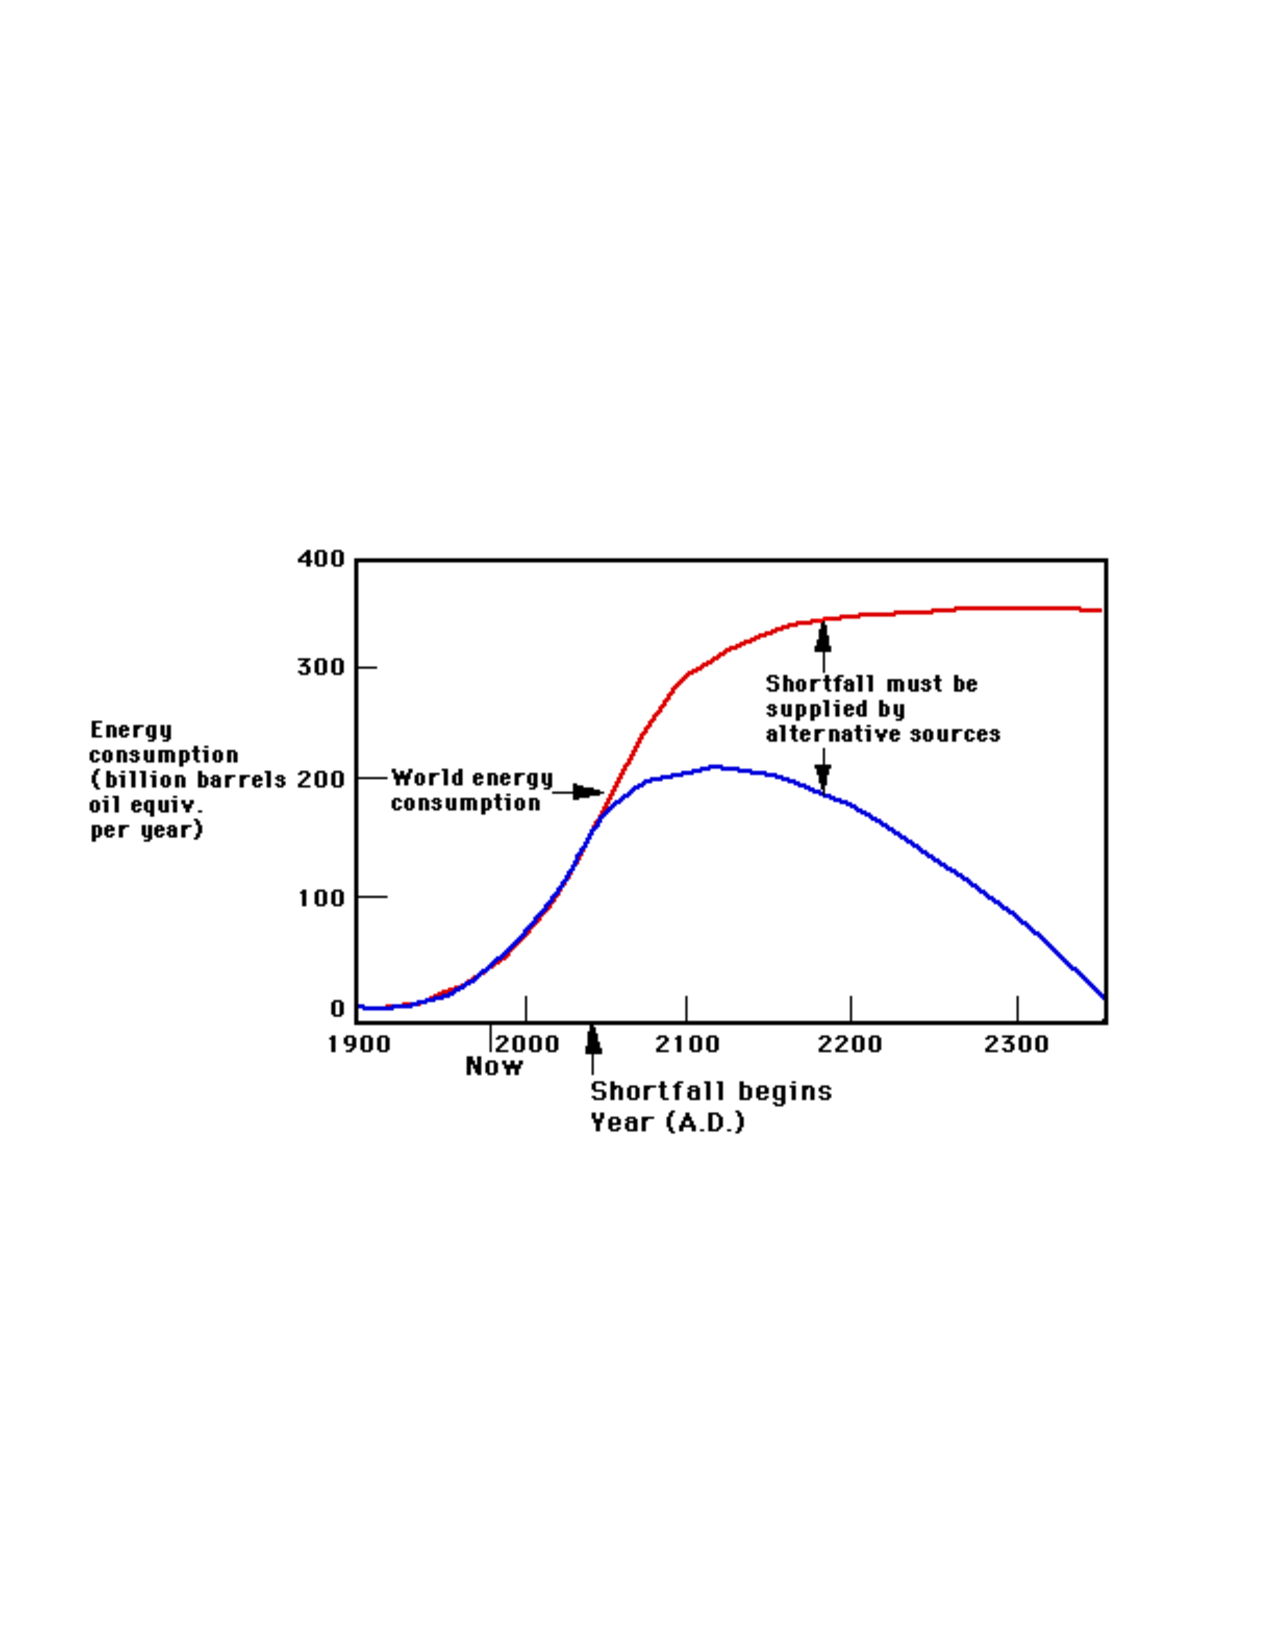
\includegraphics[width=\linewidth]{projected_energy_shortfall.pdf}
\caption{Planned energy shortfall. (Figure courtesy of Lawrence Livermore National Laboratory. \cite{GIEC})}
\label{projected_energy_shortfall}
\end{figure}

Renewable energy sources, such as solar and wind power are well ranked to contribute to energy needs in both mature and emerging technologies, but energy from these sources is unstable, intermittent and insufficient to satisfy our world increasing greed of power.

Nuclear fission and fusion, two opposite reactions that occur by splitting heavy atoms such as uranium or fusing light ones such as hydrogen respectively, can potentially produce enough energy to supply the world power demands. 

Although fission is a mature technology that is commercially available in all the nuclear plants, its by-products are highly radioactive and long lasting and its reactors are at risk of nuclear accidents due to large uncontrolled release of energy (Tchernobyl 1986, Fukushima 2011). Finally, the main nuclear fuel for fission, Uranium-235 or Plutonium-239 are nonrenewable resources (like all metals), non-recyclable, and not always easily exploited under economical and environmental acceptable conditions.

Fusion, on the other hand, offers undeniable advantages, and is the best candidate for an abundant and clean source of energy: no environmental pollution during operations since it releases helium, no risk of a nuclear accident since uncontrolled release of energy seen in fission cannot happen and finally a sufficient nuclear fuel supply due to the use of deuterium and lithium, both extremely abundant and easy to extract from nature. All these arguments enables us to state that fusion is the quickest energy solution available to us.

The most popular device where the fusion process occurs is called \textbf{Tokamak} and this is exactly what we will focus on for the rest of this dissertation.

Nuclei do not naturally fuse. They are positively charged so they repel each other. In order to fuse, Nuclei have to overcome this huge electrostatic repulsion before they can get close enough together such that the strong nuclear force which maintains nuclei together can kick in.

In order to overcome the natural electrostatic barrier, we have to make the fuel nuclei six to seven times hotter than the Sun's core. In fact to initiate any fusion reaction, a temperature of about 120 million degrees Celsius is required. At such extremely high temperatures, the fuel atoms are dissociated into their component electrons and nuclei, forming the fourth state of matter called \textbf{plasma}.

Keeping this plasma in one place long enough for the nuclei to fuse together is not trivial. Therefore the main idea of the tokamak device is to confine plasma using strong magnetic fields, generated by coils of electrical superconductors around a donut-shaped magnetic bottle in which the plasma is trapped: the combined effect of electric current flowing in the toroidal and poloidal field coils and in the plasma itself produces helical magnetic field lines that create a configuration from which plasma charged particles never leave the torus (inside the tokamak).

Plasmas in tokamak devices need to be confined in order to have a better fusion reaction so increasing the confinement time is a key feature as the longer the plasma is confined, the more fusion energy is extracted.

All existing tokamaks are pulsed devices which means that the plasma is maintained within the tokamak for only a few seconds to several hours (TRIAM-1M maintained a plasma discharge of over 100\,kA for over 5 hours using lower hybrid current drive). Each of these operating cycles of heating the plasma that cools down is called a \textbf{discharge} or a \textbf{shot}. One goal is to increase the duration of the shot. Today's plasma experiments in tokamaks can confine plasmas at the required temperatures for net power gain, but the plasma density and energy confinement time (a measure of the cooling time of the plasma) are too low for the plasma to be self-heated (a burning plasma).

In current fusion experiments, neutral beams, which consist of uncharged atoms of deuterium at high velocity, are being used to heat the plasma. These particles collide with the moving particles of the plasma transferring their momentum to the background plasma and eventually further heating the plasma. This is the most frequently used method of heating the plasma \cite{Stix72, Wagner82, Kaye85, Strachan87}. In fact this is an important element that we will be using in our rotation research, not only as a heater for the plasma but an important contributor of plasma rotation as during collisions, neutral beams also transfer momentum \cite{Suckewer79, Suckewer81, Strait07}. Others methods like ohmic heating through induction, or radio-frequency (RF) heating can also be used for plasma heating. We don't expand on these heating methods but more details can be found in \cite{Stix75, Fisch78, Kubo83, Goldston84}.

It is very important for safety and control to be able to monitor the different plasma properties during a shot, so we can adapt our response in real-time, and understand better how the distributions of the plasma properties behave during the experiment.

Plasma temperature is so hot inside the tokamak. Putting any measurement device during an operation can cause its evaporation or melting.
Luckily, we can rely on indirect methods of measurement and diagnostics, and we can also take advantage of our knowledge of plasma axisymmetric force balance which gives rise to magnetic flux contours and where pressure is constant. Controlling  the magnetic flux enables us to control the plasma.

The magnetic reconstruction of these inner flux contours is done using external probes measuring the localized magnetic fields and current flows. However these external measurements are not sufficient to deduce all internal parameters so they have to be complemented by measurements made using different methods. The two most frequent methods are using lasers to see how light is scattered or slowed as it passes through the plasma or sending a beam of neutral atoms through the plasma and analyzing the resulting optical emissions.
This allows us to measure temperature, pressure, density, magnetic field and current throughout the plasma. See \cite{Equipe78, Orlinskij88, Matthews94, McKee99, Hutchinson02} for more details.

\section{NSTX and NSTX-U devices}

A spherical tokamak is a type of fusion power device based on the tokamak principle. It is notable for its very low \textbf{aspect ratio}. A traditional tokamak has a toroidal confinement area that gives it an overall shape similar to a donut with a large hole in the middle. The spherical tokamak reduces the size of the hole to almost zero, resulting in a plasma shape that is almost spherical, often compared to a cored apple. The spherical tokamak is sometimes referred to as a spherical torus and often shortened to \emph{ST}. A comparison against a conventional tokamak is shown in Figure~\ref{nstx1}.

\begin{figure}[htbp]
	\centering
	\begin{tikzpicture}
		\node[anchor=south west,inner sep=0] at (0,0) {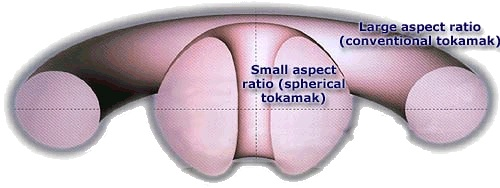
\includegraphics[width= 0.7\linewidth]{nstx}};
		\draw[red, very thick] (5.47,1.7) -- ++(down:2);
		\draw[red, very thick] (6.67,1.7) -- ++(down:2);
		\draw[red, very thick] (7.52,1.7) -- ++(down:2);
		\draw[red, thick, <->] (5.47,-.2) -- node[black, fill=white, inner sep=2pt] {$R$} (6.67,-.2);
		\draw[red, thick, <->] (6.67,-.2) -- node[black, fill=white, inner sep=2pt] {$a$} (7.52,-.2);
	\end{tikzpicture}
	\caption{Sperical tokamak vs conventional tokamak. (Figure courtesy of Culham Centre for Fusion Energy.)}
	\label{nstx1}
\end{figure}

The National Spherical Torus Experiment (NSTX)  (Fig~\ref{nstx2}) is an innovative magnetic fusion device based on the spherical tokamak concept. It was constructed by the Princeton Plasma Physics Laboratory (PPPL) in collaboration with the Oak Ridge National Laboratory, Columbia University, and the University of Washington at Seattle.

\begin{figure}[htbp]
	\centering
	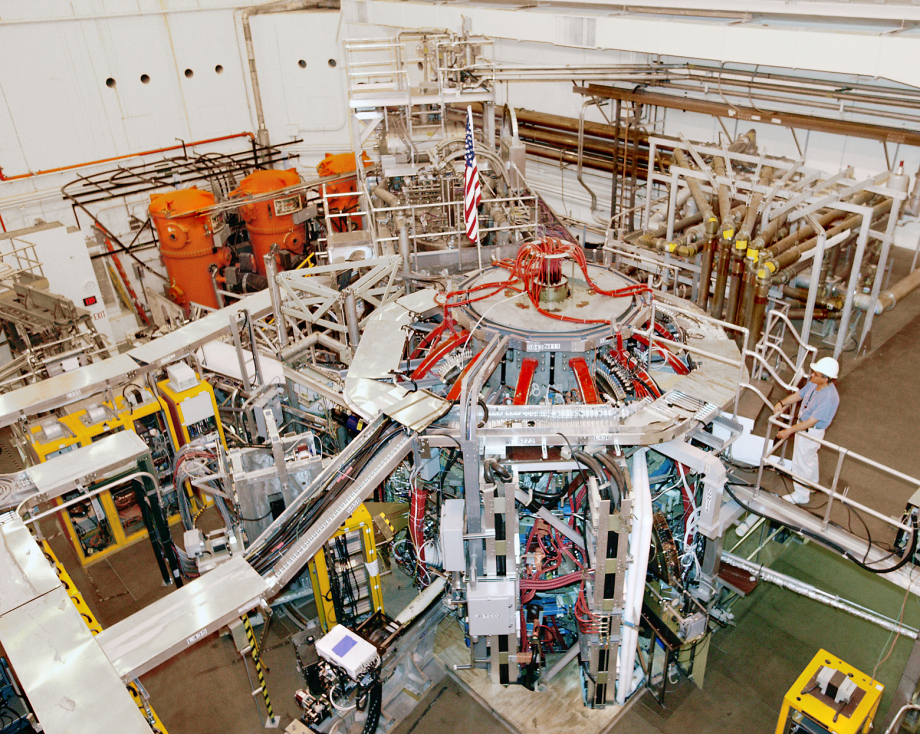
\includegraphics[width= 0.9\linewidth]{nstx2}
	\caption{Picture of the National Spherical Torus Experiment (NSTX). (Courtesy of PPPL.)}
	\label{nstx2}
\end{figure}

NSTX has a low aspect ratio of $A= R/a =1.31$, with the major radius $R =0.85$\,m and the minor radius $a =0.65$\,m.
The experimental NSTX device has several advantages including plasma stability through improved confinement, but requires a very careful design of the toroidal and poloidal field coils, vacuum vessels and plasma-facing components. Moreover, this innovative plasma configuration has the advantage of being able to confine a higher pressure plasma than a conventional tokamak of high aspect ratio for a given confinement magnetic field strength. Since the amount of fusion power produced is proportional to the square of the plasma pressure, the use of spherically shaped plasmas could allow the development of smaller, more economical and more stable fusion reactors. NSTX's attractiveness may be further enhanced by its ability to reach a high \emph{bootstrap} electric current. This self-driven internal plasma current would reduce the power requirements of externally driven plasma currents required to heat and confine the plasma.

The U.S. Department of Energy's Princeton Plasma Physics Laboratory (PPPL) runs the National Spherical Torus Experiment (NSTX), which has undergone a \$94 million upgrade which was completed in 2015 which makes it the most powerful spherical tokamak in the world. Experiments are currently testing the ability of the upgraded spherical facility to maintain a high-performance plasma under extreme heat and power conditions. Results could strongly influence the design of future fusion reactors.

\begin{figure}[htbp]
	\centering
	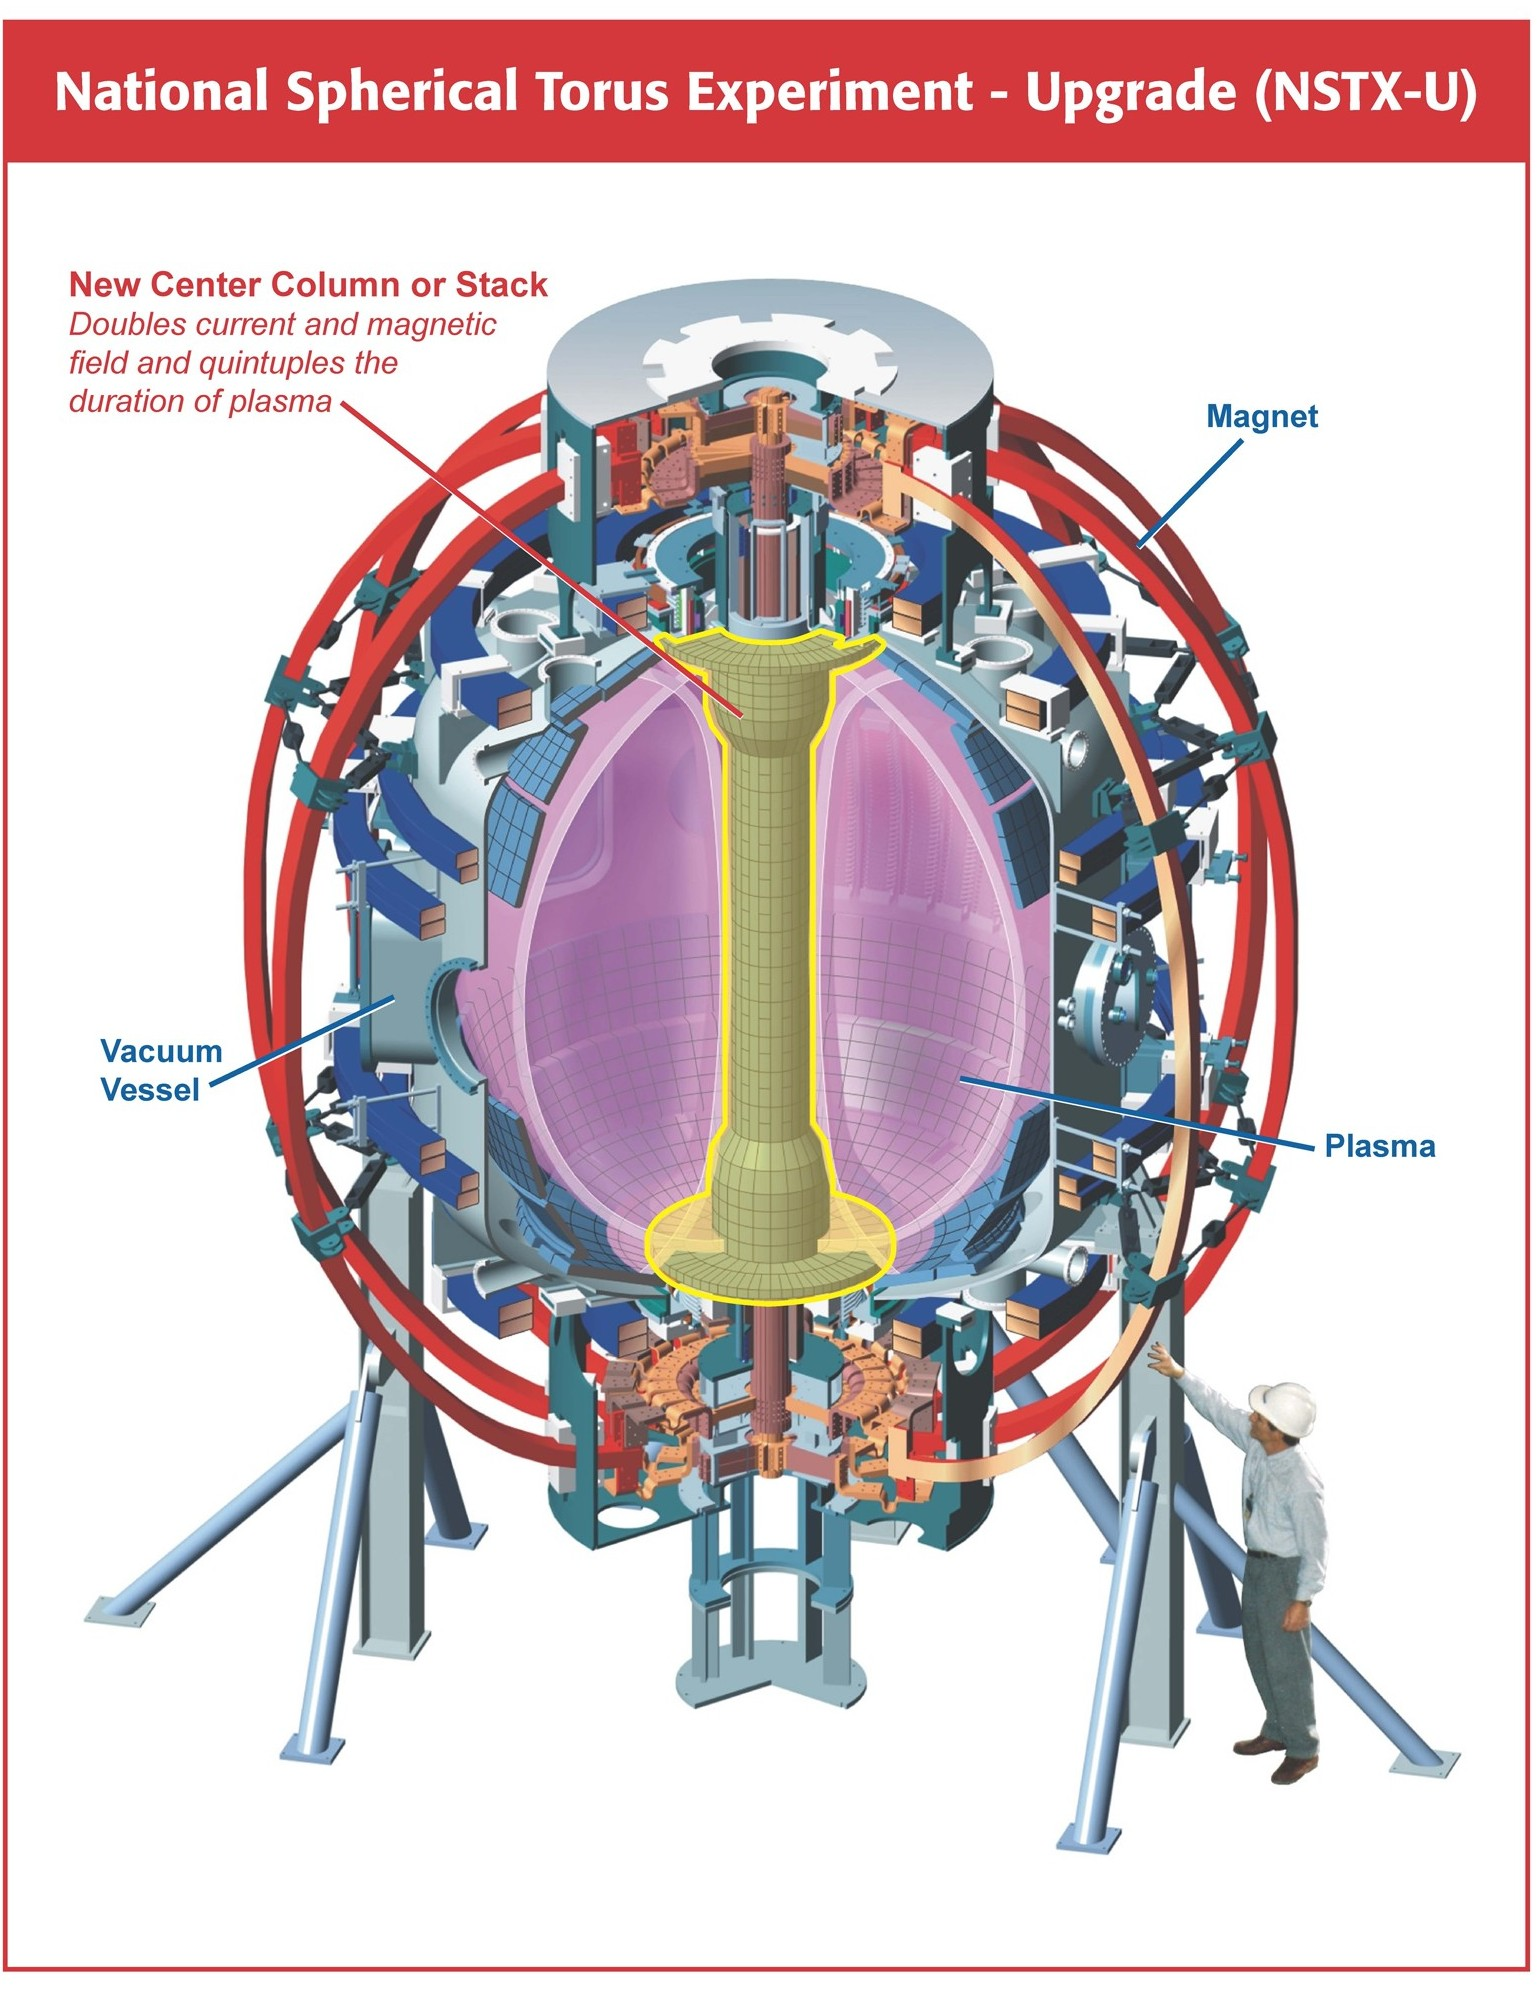
\includegraphics[width= 0.85\linewidth]{nstx3}
	\caption{NSTX-U cross section (Figure courtesy of PPPL.)}
	\label{nstx3}
\end{figure}

The primary components of the upgrade are the complete replacement of the center stack (Figure~\ref{nstx3}), (which consists of 36 22-footlong, 350-pound copper conductors which comprise the inner-leg of the toroidal field (TF) coils, the Ohmic heating (OH) solenoid, and some divertor coils), and the addition of a second neutral beam injector (Fig~\ref{nstxu}), aimed more tangentially compared to the present original set of beams, and this will give us considerably more flexibility and power to heat the tokamak.
%Temperature inside the NSTX-U exceeds the 15 million degree Celsius core of the sun and NSTX-U magnets are 20,000 times stronger than the Earth's magnetic field.

\begin{figure}[htbp]
	\centering
	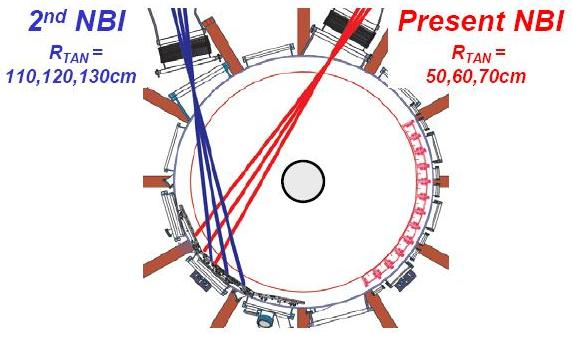
\includegraphics[width= 0.6\linewidth]{NSTXU}
	\caption{Cut-away top view of NSTX-U showing the trajectory of the neutral beams. (Figure courtesy of PPPL.)}
	\label{nstxu}
\end{figure}

\section{Various control problems in Tokamaks}

During a tokamak pulse, several things happen:
\begin{itemize}
	\item A plasma is created.
	\item The plasma is ramped up to the reference flat top current and heated to the ignition temperature needed.
	\item The plasma is cooled down (\emph{ramped down}) and terminated.
\end{itemize} 
The key step of maintaining the plasma in a current flat-top is not quite reached yet \cite{Green03}, but all the other steps are mastered. During a pulse, time variation of coil currents and plasma geometrical and physical parameters are the predetermined nominal values computed from magnetohydrodynamic (MHD) simulation codes to determine the magnetic field and plasma current density necessary for the equilibria \cite{Lao85, Takeda91, Lao05}.\\\\
%
The performance objectives in any tokamak are:
\begin{itemize}
\item High plasma temperature
\item High plasma pressure $\beta$ 
\item Long energy confinement time $\tau_E$ 
\item High driving plasma current
\end{itemize}
and all these quantities in steady state configuration. Therefore feedback control of the basic functions of plasma initiation, shaping, heating current drive, stabilization and safe termination of discharges becomes necessary especially because tokamaks often operate near the stability limits. Control is also highly needed due to uncertainty and complexity in the mathematical models of the plasma dynamics and unpredictable disturbances, and this is what makes the overall control problems very challenging and very interesting; the most desirable high performance regimes from the perspective of a fusion power reactor tend to be those that are the nearest to instability.

There have been huge accomplishments and advances in reduced-order modeling and control for plasma fusion on different tokamak devices, including vertical position control, shape control, kinetic and current profile control, MHD (magnetohydrodynamic) stabilization and plasma transport reduction.

These control engineering problems can be classified into two groups: 
\begin{itemize}
\item \textbf{Electromagnetic control:} which refers to controlling the magnetic and electric fields to regulate the position and shape of the plasma, as well as the total plasma current. 

\item \textbf{Kinetic control:} which refers to controlling fueling rates and auxiliary heating to modify the plasma density, temperature, and pressure.
\end{itemize}
This section addresses these different control problems and gives an short overview of the methods used on different tokamaks for each control problem.

\subsection{Electromagnetic control}

\subsubsection{NTM control}
In a high pressure resistive plasma, nested magnetic surfaces can go unstable by tearing and reconnecting with each others. This creates magnetic islands which connect hotter core regions of the plasma to colder regions. This phenomena known as the Neoclassical Tearing Mode NTM is a short circuit effect that drives the plasma heat to leak out of the core, creating a flattening in plasma temperature, pressure and current profile and results in bad confinement and plasma disruption.
%NTM can be caused by seed islands growing from ELMs instabilities or by background plasma turbulence, which can be impossible to eliminate. 

The fundamental idea of NTM suppression comes from experimental observations and it is done through active control laws that use highly localized Electron Cyclotron Current Drive (ECCD) to compensate for the plasma current loss. Restoring the current drive would shrink these magnetic islands, restore the nested flux surfaces and stabilize the mode.

In DIII-D for example, a plasma control system based on a ‘‘search and suppress’’ algorithm (active tracking and target lock routines) was able to make either small rigid radial position shifts of the entire plasma or small changes in the toroidal field to find and lock the optimum position for complete island suppression  \cite{Haye02}. 
%This was based on real-time measurements and the experimental tests showed the first use of active feedback control to provide continuous precise positioning for NTM control. 

While NTM control in tokamaks is still in constant progress, it benefited from advances in control algorithms, estimation, real-time computation, actuator technology and diagnostic signal interpretation \cite{Bongers09, Volpe09, Zohm07}.

Another example, in the ASDEX Upgrade device \cite{Rapson13, Rapson14}, the NTM dynamical system (a second order damped system) was simulated in SIMULINK and an anti-windup Proportional-Integral (PI) controller was designed and tuned (optimized) through various simulation in order to obtain the best system performances. 
The controller was designed such that it tries to generate invalid input commands, the mode of operation switches to a fallback mode which requires no inputs and is safe by design. It returns to normal functionality if all input commands are valid again. This functionality which is included as part of a standard feature within the ASDEX Upgrade control system bears resemblance with how we handle invalid input commands in our rotation controller where the inputs (beam powers and coil current) cannot exceed a certain physical threshold.

\subsubsection{ELM control}
An Edge Localized Mode (ELM) is a disruptive instability occurring in the edge region of a tokamak plasma when it is heated above a certain power level (high energy confinement, H-mode). ELMs can cause a loss of up to 10\% of the total plasma stored energy on a very short timescale. Therefore, the control of ELMs is an important issue to consider.

A standard ELM control technique consists of imposing a high critical threshold of pressure gradient to the plasma, and keep the input power low so that this critical threshold is not reached.
The drawback of this technique is that ELMs can be beneficial as they naturally reduce the sources of impurities, thus totally suppressing them would provoke an accumulation of impurities that can deteriorate the plasma confinement.
An ideal control strategy would allow to eliminate the ELMs while providing an alternative method for reducing these impurities through density control. There are no sufficiently advanced methods using a feedback control approach yet but many experimental control approaches that have been tested. For example, injecting deuterium pellet for the ASDEX-U or DIII-D tokamaks \cite{Kallenbach05, Loarte14} or controlling by 3D edge magnetic field perturbations \cite{ Loarte14} all allow a significant reduction of ELMs.

\subsubsection{RWM control}
The Resistive Wall Mode (RWM) is one of the major tokamak non-axisymmetric instabilities.

Active feedback of RWMs in tokamaks was investigated in \cite{Fransson00} using control
theory. Control systems were designed to stabilize the resistive wall mode and meet certain performance specifications for a set of test equilibria. A control problem for $n > 0$ RWMs in tokamaks (through system identification) was formulated then several different controllers: P (proportional), PD (proportional-derivative) and $H_{\infty}$ were applied.

\cite{Garofalo01} for DIII-D and  \cite{Sabbagh04} for NSTX applied similar active feedback control of RWM approaches based on simulation and experimental tuning of the controller gains to meet some performance requirements.

A combined algorithm for resistive wall mode identification using both a matched filter and a Kalman filter was implemented in the DIII-D plasma control system (PCS) \cite{In06}. The Kalman filter was based on an eigenmode approach which is similar to our model-based reduced-order control approach, it enables to build a low dimensional controller with an observer takes advantage of the relevant magnetic sensors used for measurements. 

\subsubsection{Vertical position control}
It has been proven theoretically that plasmas with a vertically elongated cross section improve and increase energy confinement time, and the first experiments performed in the seventies on tokamaks confirmed these theoretical predictions \cite{Pironti05,Robinson78}. A vertical elongated plasma implies a vertical axisymmetric MHD instability that can be stabilized by surrounding the plasma with a superconductive wall \cite{Mori87, Okabayashi74, Blum81} and applying an active feedback system \cite{Rebhan78}. A detailed investigation of techniques for active stabilization of elongated plasmas can be found in Humphreys and Hutchinson's work on the Alcator C-Mod device \cite{Humphreys89}.

The problem of plasma vertical position stabilization and shape control under actuation saturation in the DIII-D Tokamak at General Atomics was studied in \cite{Schuster03} where an anti-windup compensator was designed for a given predesigned nominal plasma vertical position controller guaranteeing global vertical stabilization of the plasma in the presence of actuator saturation for all reference commands.

\subsubsection{Current profile control}
One of the first work on current control has been the work of Gran \cite{Gran77} on the TFTR device (the ancestor of NSTX), where a control system design has been developed using linear optimal control techniques. On that work, both the ohmic heating and equilibrium field coils were controlled to maintain plasma current and plasma position at their desired values.
Due to its effect on confinement, plasma stability, and non-inductively driven plasma current, the control of current profile became critical and a huge advancement in controlling this profile has recently been made on several machines.

For JET \cite{Moreau03, Moreau08, Laborde05}, a system identification procedure has been developed, a system discretization was therefore performed through an expansion onto a finite set of appropriate basis functions and a Galerkin scheme and a state space model structure was obtained. A combining control law of a slow (proportional + integral) and a fast (proportional) feedback loop was then designed to reach the closest self consistent achievable state defined by the minimization of a quadratic integral error.

For DIII-D, \cite{ Boyer13} has designed a current profile controller using a first-principles-driven dynamic model (with minimal parameters determined from experiment). The feedback controller was designed to complement any arbitrary set of feedforward inputs and drive the spatial profile to the desired target profile (reference tracking). Through a nonlinear transformation of the inputs and spatial discretization, a finite dimensional, time-varying linear model for the profile error was obtained. A singular-value decomposition (SVD) technique was used to reduce the multiple input multiple output (MIMO) coupled system to a set of the most relevant control system. A linear-quadratic-integral (LQI) controller was then designed for the reduced order model. 

This control approach used is very similar to our rotation control strategy which builds its simplified momentum model from a dynamic model (with some experimentally deduced parameters), uses linearization and model reduction as well (projections on Bessel functions) and builds the corresponding reduced optimal controller (LQG) which contains an integrator, an anti-windup but also an observer (Kalman filter) which enables us to rely on inputs and outputs measurements only while taking feedback actions.

Another method (nonlinear PDE control) consisting of using a backstepping boundary control technique has also been applied to current profile control in \cite{Boyer14}. In this work, a backstepping current profile control algorithm (PI controller) was designed for the DIII-D tokamak. This control design technique provided a systematic method to obtain a boundary feedback law through the transformation of a spatially discretized version of the original system into an asymptotically stable target system with desirable properties. 

Motivated by the current profile control, in \cite{Xu11}, the authors consider a 1D parabolic system which is similar to our considered diffusion equation for rotation control. A Proper Orthogonal Decomposition (POD) reduced order model was derived and a reduced order bilinear system was obtained. A convergent successive scheme to compute the solution of a finite-time suboptimal control problem defined for this latter reduced order bilinear system was then designed.
The drawback of this method is that it requires to numerically solve a number of ODEs (Riccati equations) at each iteration of this algorithm whereas our method of linearizing the bilinear term enables us to simply solve the Riccati equation once and reuse the results (gains) through all iterations.


 \subsubsection{{Shape control}} 
To optimally use the space and to ensure good stabilization in large highly elongated tokamaks, the plasma must be maintained as close as possible to the surrounding walls, thus in addition to a vertical control and a plasma current control, an accurate shape control becomes necessary. Because the coil for ohmic heating, the coil for the vertical and radial fields and the coil for the shaping field are usually the same or partially jointly used, this creates a coupling in the input and output parameters of the control systems and therefore adds more complexity to the problem.

In \cite{Gates05}, plasma shape control using real-time equilibrium reconstruction has been implemented on NSTX. The real-time equilibria provide calculations of the flux at points on the plasma boundary, which are used as input to a shape control algorithm known as isoflux control. The flux at the desired boundary location is compared with a reference flux value, and the difference is used as the basic feedback quantity for the poloidal field coils on NSTX.

More recently, \cite{Kolemen11} gives an overview of the shape control implementations and dynamics studies  performed on NSTX, in particular, strike point position and X-point height control.
A PID controller for the strike point was tuned by analyzing the step response of the strike point position to the poloidal coil currents, employing the Ziegler-Nichols method. A system identification of the plasma response to the control inputs was used to build the model. An online automatic relay-feedback PID tuning algorithm was then designed.


\subsection{Kinetic control}


\subsubsection{{Burn control}} 
To become an economical alternative energy source, nuclear fusion tokamaks must be capable of operating for extended periods of time in a burning plasma mode characterized by a large value of $Q$, the ratio of fusion power to auxiliary power, in other words, we ideally want more ``power out'' than ``power in''. Achieving and maintaining such conditions requires precise control over the plasma density and temperature.

Modulation of the auxiliary power, modulation of the fueling rate, and controlled injection of impurities are considered as possible actuators for the burn control.

In \cite{Mitarai10}, a PID control law was used to regulate fusion power using the deuterium-tritium fueling rate.
In \cite{Leonov05}, a diagonal multi-input, multi-output linear control scheme for burning plasma kinetics was developed by observing actuator influences during numerical simulations of plasmas.
The approximation of the nonlinear burning plasma model by a linearized one for controller design is a common denominator in many model-based controller designs. The model is linearized, a controller is synthesized using linear techniques, and the resulting design is tested on the original nonlinear model. 
These controllers succeed in stabilizing the system in nonlinear simulations against a limited set of perturbations and disturbances.

In \cite{Schuster03}, a nonlinear model involving approximate conservation equations for the energy and particles densities was used to synthesize a nonlinear feedback controller (a nonlinear backstepping algorithm) for burn conditions stabilization. The use of nonlinear control techniques removes the limits imposed by linearization and the resulting controller can accommodate very large perturbations but its implementation and applicability on the PCS are not straightforward and requires several iterations whereas linear controller are standard, simple and more adaptive to other control problems.

\subsubsection{{Rotation control}} 

In an operating tokamak, each particle has its own velocity and the net sum of velocities of a particle species is the fluid velocity of that species. This fluid velocity can be separated into components; parallel and perpendicular to the flux surfaces. The velocity perpendicular to a flux surface is called convection, and the velocity parallel to the flux surface is called \textbf{rotation}.

We will consider here the toroidal (parallel) component of the velocity $V_{\phi}$ and its angular frequency $\omega = V_{\phi} / R$ where $R$ is the plasma major radius.

Plasma toroidal rotation and its shear have been recognized as a stabilizing mechanism for magnetohydrodynamic (MHD) instabilities such as the neoclassical tearing mode (NTM) \cite{LaHaye10} where a reduced plasma rotation experimentally destabilizes these NTMs at Lower $\beta$ in the DIII-D, NSTX and JET devices by minimizing the effect of error fields that excite these tearing modes. It also helps prevent the resistive wall modes (RWM) \cite{Garofalo02} where these long-wavelength modes are stabilized by a rapid plasma toroidal rotation.
High plasma rotation can have a significant impact on the plasma confinement time by suppressing energy and particle transport to the walls.

\textbf{Neutral beam injection} (NBI) is the dominant source of momentum and therefore rotation in present-day tokamaks. NBI consists of injecting beams of highly energetic neutral particles into the plasma, heating the plasma through collisions, and naturally transferring momentum. 

%The NBI system at DIII-D for example, consists of eight beam-lines, each of which can inject a maximum of $2.5$ MW of power into the plasma, four of them are designed to inject in the same direction as the plasma current, aligned with the magnetic axis, two of them are designed to drive co-current with alignment off-axis, and the last two beams are designed to inject in the opposite direction of the plasma current with on-axis alignment. 

The NBI system of NSTX (resp. NSTX-U) considered in this work consists of one set (resp. two sets) of three beams which can each inject a maximum of 2\,MW of power into the plasma. Its configuration is shown in Fig~\ref{nstxu} and its injection is spread throughout the plasma flux surfaces which ensures a rotation drive across the plasma poloidal profile. 

Several mechanisms have been developed to control and affect plasma rotation beside the main external source of neutral beams injection as toroidal rotation can be influenced by the intrinsic rotation and the 3D magnetic fields due to MHD instabilities or field errors.

The experimental work done in \cite{Solomon10} for example focuses on investigating mechanisms of driving rotation in fusion plasmas without external momentum input (use of intrinsic rotation and non-resonant magnetic fields). It has been found that the torque from these fields can be enhanced at low rotation, which assists in spinning the plasma from rest, and offers increased resistance against plasma slowing.
In this dissertation, we will focus exclusively on the neutral beams injection as the unique source for driving toroidal rotation. All other sources will not be considered.

Rotation control in tokamaks has been already demonstrated using momentum input from injected neutral beams (NBI) as actuators \cite{Scoville07, Yoshida09}.

\cite{Yoshida09} controls the combined ion temperature profile and toroidal rotation for JT-60U device experimentally using real-time measurement and real-time control system consisting of a tuned PID controller.

In \cite{Scoville07}, simultaneous control of the rotation and stored energy was considered for the DIII-D device. In this work,  a model-based control algorithm for simultaneous regulation of plasma rotation and $\beta$ has been developed and casted in linear state space form then combined with a proportional-integral-derivative (PID) transfer function to form a closed loop control algorithm which then has been used by the PCS for experimental testing. Our work will show similarities in controlling both the rotation and the stored energy with \cite{Scoville07} but will use a different methodology (model reduction and an optimal controller). More details in the following section.

\section{Contribution of this dissertation}

The main subject of this thesis is to explore \textbf{toroidal rotation profile control}  in tokamaks through its direct application on NSTX and NSTX-U devices. 
The methodology used throughout the thesis relies heavily on the mechanical engineering tools that are very commonly used in fluid mechanics and flow control such as model reduction and linear feedback controllers. The idea here is to transpose this knowledge and tools and apply them to control the toroidal rotation of plasma in tokamaks. 

The thesis begins with a classical plasma problem as a preliminary case study where this methodology of reduced order modeling and control is applied to demonstrate the effectiveness and applicability of our tools. 

We then focus on the main topic which is the control of plasma toroidal rotation in a tokamak, to maintain plasma stability for long-pulse operation. We use experimental measurements from the National Spherical Torus Experiment (NSTX) and two different types of actuation: momentum from injected neutral beams and neoclassical toroidal viscosity generated by three-dimensional applied magnetic fields. 

Whether based on the data-driven model obtained for NSTX or pure modeling for NSTX-U, a feedback controller is designed, and predictive simulations using the TRANSP plasma transport code show that the controller drives the plasma rotation to various desired profiles given practical constraints on the actuators and the available rotation measurements. Another application of simultaneously controling the toroidal rotation profile and $\beta_n$ stored energy is shown for NSTX-U as well. 

The approach used in this dissertation for NSTX-U is quite similar to the one used in \cite{Scoville07} for DIII-D  except that the new and unique aspect of it is the use of non-axisymmetric (three-dimensional) magnetic fields as another actuator in closed-loop feedback control to supplement the neutral beam actuator. Rotation alteration by non-resonant, three-dimensional magnetic fields allows more precise, continuous control of the plasma rotation than NBI, as the momentum delivered by the latter occurs in significantly large, discrete increments.

The modeling and control design of the plasma rotation differ also from \cite{Scoville07}. Starting from a diffusion equation, we first proceed to linearize it, then we apply model reduction on it in order to reduce the dimension of the state of the linear optimal controller (LQG) which is a more sophisticated design as it contains both an observer and an integrator. \cite{Scoville07} does not reduce the model but designs a PID controller tuned through rotation simulations. A model-based controller enables us to tune all the gains of the controller offline and therefore drastically reduce the experimental testing.

Furthermore, using TRANSP to test a reference tracking controller for the rotation profile (and stored energy) has never been done before, and it gives confidence in the control design before experimental testing.

Our strategy for NSTX/NSTX-U rotation control is to obtain practical, low-complexity dynamical models useful for implementing relatively simple controllers for tokamaks that can be implemented in the PCS and easily be applied to experiments. Because our starting equation is bilinear like the one considered in \cite{Xu11}, the linearization strategy enables us to use the standard linear optimal control tools that can adapt to any other type of control.

Finally, in our work, a study of the robustness of the controller to some parameters uncertainties, in particular the perpendicular momentum diffusivity profile $\chi_{\phi}$ and the confinement time $\tau_e$  is performed. This will bring more confidence in the controller's robustness in stability and performance as experimental testing is not currently available for rotation control.

\section{Organization of Part I}

\textbf{Chapter 2:} We will present and explain all the background and the tools used in this thesis for the model reduction and the controller design. This will include the balanced truncation and the Bessel functions decomposition for the reduced-order modeling and the different controller designs such as model-based feedback control design and the observer control design. The methodology consisting of doing a model reduction then building a matching controller will be applied to all our plasma control problems.

\textbf{Chapter 3:} We will present our results on the first application of control on a simple plasma drift waves problem as a preliminary case study where the approach defined in chapter 2 of reduced order modeling and control is applied to demonstrate the effectiveness and applicability of our tools.

\textbf{Chapter 4:} This chapter gets into the main topic which is the control of plasma toroidal rotation in the NSTX and NSTX-U tokamaks.
It uses experimental measurements from the NSTX device but will extend the approach to NSTX-U by relying on numerical models and  simulations and eventually will increase the complexity by trying to control the rotation and the stored energy simultaneously.

\textbf{Chapter 5:} We summarize our results and possible future directions for this research.


\chapter{Background: Reduced-order modeling  and feedback control for linear time invariant systems}
\label{chapitre2}

\section{Overview and motivation}

From the numerical simulation point of view, research problems in plasmas in tokamaks are very challenging due to complex and highly nonlinear dynamics described by coupled multi-variate differential equations in a multi-parameter operating space.

There are generally no analytical solutions available to describe different phenomena occurring in a plasma due to the complexity of interference of different dynamics at the same time. However there are some model simplifications that enable us to understand some properties better; for instance, considering a plasma as a fluid (gas) enables us to state that the pressure is proportional to the product of density and temperature by the thermodynamic equation $P \propto n T$. Even if these quantities are not homogeneous within plasmas, it gives us the intuition needed to understand that the plasma in the tokamak is hotter and denser at its core thus the pressure is also higher at the core.

Another example is the ideal magnetohydrodynamics (MHD) theory which describes the basic behavior of the plasma as a perfectly conducting fluid without distinguishing the different particles composing this fluid. This approximation is sufficiently accurate to be used as a first approximation in almost every magnetic analysis done for tokamak plasma physics, including studies of instabilities and estimation of the plasma shape and position.

A very general and useful approximation technique is model reduction: a mathematical tool derived from control theory and dynamical systems which allows to extract the key coherent structures of these plasma problems and drastically simplify them. This is what we are going to describe and use in this thesis: reduction and reconstruction methods with their direct application to simulation and control of plasma in tokamaks.

This tool was extensively developed primarily for fluid dynamics problems especially flow control where, as in plasma physics, closed-form analytical solutions are rarely available for engineering applications. Mathematical tools have been developed using ideas from dynamical systems, control theory, and geometric mechanics, in order to extract some key structures and conservation laws while simplifying the original problems.

The idea arose when researchers were focusing on flow control when trying to reduce some undesired properties such as drag or instabilities (vibrations) or to enhance other ones. Major breakthroughs have been made in feedback active control due to the increase of machine capacity in simulations and modeling \cite{ Kim07, Cattafesta08, Choi07, Sipp10} thus the focus shifted to model based feedback control methods but the drawback of these methods was that it was applicable only for limited dimension systems (not bigger than $10^4$) whereas dynamical models in computational fluids dynamics dimensions were typically higher (over $10^5$). 

Therefore, having a reduced-order model that captures the main low dimensional dynamical structure (when it exists) that accurately reconstructs the input-output dynamics of the full original model is a popular solution used in flow control to solve the problem of high dimensionality. Based on the reduced model, a feedback controller is designed for the full system. Many applications of this methodology can be found, applied to various problems such as noise reduction in cavity flow \cite{Rowley05} or stabilization of an unstable steady state in \cite{Ahuja10}.

In our case, we consider the plasma in a tokamak as an ideal conducting fluid flowing in a torus and, by analogy, we will apply the same mathematical methods of model reduction and model-based feedback control to plasma problems to show its validity and efficacy. 
Reduced order methods enable us to gain computational and experimental time and focus on the main dynamics that will matter for our problems. 

The development of engineering tools for automatic regulation and control of a system's behavior never stopped progressing especially in the last several decades.

As this work will only focus specifically on linear time invariant (LTI) control theory, where we assume that plants (i.e., systems to be controlled) and controllers have linear dynamics that do not change with time. Although the LTI assumption is restrictive, the control theory tools specific to it are very standard and easy to apply. 

In this chapter, Section~\ref{standard} reviews some standard reduced-order modeling methods for Linear Time Invariant (LTI) systems. Section~\ref{optfed} reviews the standard linear feedback control methods.
These methods are used in Chapter~\ref{chapter7}, Chapter~\ref{rot1&} and Chapter~\ref{rot2&}. 

%Subsection~\ref{Besselmeth} highlights the Bessel decomposition method that is used in both Chapters~\ref{rot1&} and \ref{rot2&}.


\section{Standard reduced-order modeling methods}
\label{standard}
In this section, various standard techniques for constructing reduced-order models are briefly reviewed  for the model reduction of LTI systems used in this thesis.

\subsection{Projection-based model reduction}
This method involves the projection of a model onto a set of modes and is a widely used approach. It is sometimes called the Petrov-Galerkin projection approach.

We start by defining a stable linear time-invariant state-space system as follows: 
\begin{equation}
\label{lti1}
\begin{aligned}
	\dot{x}&= A x  + B u,   \\
	y &= C x ,
\end{aligned}
\end{equation}
where $x \in \mathbb{R}^n$ is the state (for instance, the state variables at all  grid points of the simulation), $u \in \mathbb{R}^p$ is a vector of inputs (for instance, actuators or disturbances), and $y \in \mathbb{R}^q$ is a vector of outputs (for instance, sensor measurements, or other measurable quantities as linear functions of the state). $A \in \mathbb{R}^{n \times n}$, $B \in \mathbb{R}^{n \times p}$, and $C \in \mathbb{R}^{q \times n}$ are respectively the dynamics, control and sensor matrices.

This system of equations (\ref{lti1}) is asymptotically stable if and only if all the eigenvalues of $A$ are located in the left half plane (i.e., they all have negative real parts). It is neutrally stable if it is stable and any eigenvalue of $A$ is on the imaginary axis (pure imaginary), and it is unstable if any eigenvalue of $A$ is in the right-half plane (positive real part).

The goal of model reduction is to obtain an approximate model that captures the dynamic relationship between the inputs $u$ and the outputs $y$ with the smallest dimension possible, so we can write:
\begin{equation}
\label{linSS3}
\begin{aligned}
	\dot{x_r}&= A_r x_r  + B_r u,   \\
	y &= C_r x_r ,
\end{aligned}
\end{equation}
where the reduced state variable $x_r \in \mathbb{R}^r$ and $r \ll n$, $A_r \in \mathbb{R}^{r \times r}$, $B_r \in \mathbb{R}^{r \times p}$, and $C_r \in \mathbb{R}^{q \times r}$ are respectively the corresponding reduced dynamics, control and sensor matrices.

The standard projection approach obtains the reduced order model (\ref{linSS3}) by projecting the model (\ref{lti1}) onto a $r$-dimensional subspace spanned by the columns of a matrix $\Phi_r \in  \mathbb{R}^{n \times r}$ along a direction that is orthogonal to a $r$-dimensional subspace spanned by the columns of another matrix $\Psi_r \in  \mathbb{R}^{n \times r}$. The bases  $\Phi_r$ and  $\Psi_r$ are bi-orthogonal:
\begin{equation}
\label{linSS4}
\Psi_r^{\dagger} \Phi_r = I_{r \times r},
\end{equation}
where the dagger $\dagger$ denotes the adjoint operator. 

By approximating the original state as $x \approx \Phi_r x_r$ in (\ref{lti1}) and applying the orthogonal property (\ref{linSS4}), we can deduce the reduced-order model of the form:
\begin{equation}
\label{linSS5}
\begin{aligned}
	\dot{x_r}&= \left(\Psi_r^{\dagger} A \Phi_r \right) \,x_r  + \left( \Psi_r^{\dagger} B \right) \, u,   \\
	y &= \left( C  \Phi_r \right) \,x_r.
\end{aligned}
\end{equation}
This bi-orthogonal projection approach can also be used to reduce nonlinear systems, and if $\Phi_r = \Psi_r $, this method is just an orthogonal Galerkin projection. 

We can have various projection-based model reduction methods that use different bases $\Phi_r$ and $\Psi_r$ modes and generate different reduced-order models, but the basic projection idea remains the same for all these techniques.  


\subsection{Bessel functions}
\label{Besselmeth}

One of the orthogonal Galerkin projection method that we used in this work for rotation control (Chapters~\ref{rot1&} and~\ref{rot2&}) is choosing the Bessel functions as our projecting basis functions. We then write the approximate state in (\ref{lti1}) as
\begin{equation}
x(\rho,t)  \approx \sum_{n=1}^{r} a_n (t) \varphi_n(\rho),
\label{decomp1}
\end{equation}
where $\rho$ and $t$ represent the space and time variables. The basis functions are given by
\begin{equation}
  \label{decomp2}
  \varphi_n(\rho) = J_0(k_n\rho),\qquad n=1,\ldots,r,
\end{equation}
where $J_0$ denotes the Bessel function of the first kind and $k_n$ denotes the $n$-th root of $J_0$. Furthermore, the basis functions satisfy the orthogonality relation
\begin{equation}
  \label{decomp3}
  \langle \varphi_n,\varphi_m\rangle = 0,\qquad \text{for $m\ne n$},
\end{equation}
where the inner product is defined by
\begin{equation}
\langle f,g \rangle =   \int^1 _0 \rho \, f(\rho) \, g(\rho) \, d\rho.
\end{equation}
 Inserting the expansion~\eqref{decomp1} into~\eqref{lti1} then taking the inner product with~$\varphi_m$, and using the orthogonality relation~\eqref{decomp3}, we obtain the following reduced-order system
% 
\begin{equation}
\begin{aligned}
  \dot a_m &= \sum_{n=1}^r \frac{\langle A  \varphi_n,  \varphi_m\rangle}{\langle \varphi_m,\varphi_m\rangle} a_n +\frac{ \langle B u,\varphi_m\rangle}{\langle \varphi_m,\varphi_m\rangle} ,\\
    y &= C \sum_{n=1}^{r} a_n (t) \varphi_n(\rho)
\end{aligned}
\end{equation}
where $ m=1,\ldots,r$ which is a set of $r$ coupled ordinary differential equations for the coefficients $a_m$. Note that the reduced state becomes a vector of coefficients obtained from the projection of the non reduced state onto the Bessel functions basis.

\subsection{Balanced truncation method}
\label{baltrun}

For systems like (\ref{lti1}), the concepts of controllability and observability can be defined and quantified by a pair of symmetric, positive-semidefinite matrices
\begin{subequations}
\begin{align}
W_c  &= \int_0 ^{\infty} e^{At} B B^{\dagger}  e^{A^{\dagger}t} dt, \\
W_o  &= \int_0 ^{\infty} e^{A^\dagger t}  C^\dagger C  e^{At} dt, 
\end{align}
\label{obscontr}
\end{subequations}
called controllability and observability Gramians. The dagger $\dagger$ denotes the adjoint operator. 

 The controllability Gramian~$W_c$ provides a measure of the influence of input history on the current state (i.e,\ to what degree each state is excited by inputs), and the observability  Gramian~$W_o$ measures the influence of an initial state on future outputs with zero control input (i.e,\ to what degree each state excites future outputs). The larger eigenvalues of the controllability (observability) Gramian correspond to the more controllable (observable) states.

We then define the Hankel norm of a system $G$ (defined by its state space realization (\ref{lti1})) as the maximum ratio, over all input signals, between an output signal norm and the given input signal norm
\begin{equation}
\| G \|_H = \sqrt{ \max \, \text{eig}(W_c W_o) } = \sqrt{ \max \, \text{eig}(W_o W_c) },
\end{equation}
we also define the $j$th Hankel singular value $\sigma_j (G)$ as the square root of the $j$th eigenvalue of $W_o W_c$ (or $W_c W_o$ ) with the ordering
\[
	\sigma_1(G) \ge   \sigma_2(G) \ge \cdots \ge \sigma_j (G) \ge \cdots.
\]


A balanced truncation involves first a coordinate transformation $T$, called the balancing transformation, that simultaneously diagonalizes the controllability and observability matrices defined by \eqref{obscontr}.  That is, under a change of coordinates $x=Tz$, the transformed Gramians become

\begin{equation}
T^{-1} W_c ( T^{-1} )^\dagger = T^{\dagger} W_o  T = \Sigma,
\end{equation}
where $\Sigma = \operatorname{diag}(\sigma_1,\ldots,\sigma_n)$ is a diagonal matrix which its diagonal entries are the Hankel singular values ordered so that $\sigma_1 \ge \cdots \ge \sigma_n \ge 0$.

A reduced-order model may then be obtained by truncating the states that are least controllable and observable.  That is, if $T = \bigl[ T_1\ \,T_2 \bigr]$, and $x = Tz = T_1 z_1 + T_2 z_2$, then a reduced-order model is obtained by setting $z_2=0$, yielding a model of the form
\begin{equation}
\label{redz2}
\begin{aligned}
	\dot{z}_1 &= A_r z_1  + B_r u,   \\
	y &= C_r z_1 ,
\end{aligned}
\end{equation}
The resulting reduced-order balanced model retains the most controllable and observable states and is therefore suitable for capturing the input-output dynamics of the original system.

Quantitatively the balanced truncation procedure guarantees an a priori analytical upper bound of error between the original system and the reduced-order model.  If $G(s)=C(sI-A)^{-1}B$ denotes the transfer function of the system~(\ref{lti1}), and $G_r(s)$ denotes the corresponding transfer function of the approximation~(\ref{redz2}), then 
\begin{equation}
\label{ineq1a}
|| G - G_r||_{\infty} < 2 \sum_{k= r+1} ^n \sigma_r.
\end{equation}
In addition, any reduced-order model $G_r$ with $r$ states satisfies 
 \begin{equation}
 \label{ineq2b}
|| G - G_r||_{\infty} > \sigma_{r+1},
\end{equation}
where $ \sigma_{r+1}$ is the first neglected Hankel singular value of $G$. This is a fundamental limitation for any reduced-order model. The two inequalities (\ref{ineq1a}) and~(\ref{ineq2b}) provide error bounds.
More details of this method can be found in \cite{Glover84} and \cite{SandP}.

In Chapter~\ref{chapter7}, we applied the balanced truncation method to the Hasegawa-Wakatani (HW) problem in order to build the reduced order model. However for a certain set of parameters, the HW system exhibited some unstable modes (its dynamics matrix $A$ has some unstable eigenvalues, also called right half plane poles).

Because the balanced truncation method only applies to stable models, we could not apply it directly to our HW problem. An extension for unstable models does exist and consists of first decomposing the model into a stable and unstable submodels.

For instance, we can write a system as a sum of two subsystems
\begin{equation}
G(s) = G_u(s)+ G_s(s),
\end{equation}
where $G_u$ contains all the unstable poles (eigenvalues of $A$ with a non-negative real part), and $G_s$ contains the stable ones (eigenvalues of $A$ with a negative real part).

The balanced truncation can therefore be applied to the stable part of the system $G_s$ to find a reduced order approximation $G_{s \, r}$
which can then be added to the unstable subsystem to obtain an approximation of the full model $G(s)$
\begin{equation}
G(s) = G_u(s)+ G_{s \, r}(s).
\end{equation}


\subsection{Methods for high dimensional systems}
\label{highdim}

The fluid mechanics community has been precursor in developing high dimensional reduced-order modeling methods due to the extremely high state sizes needed for the conversion of partial differential equations to ordinary differential equations: modeling flows of fluids requires state sizes of the order of $10^{\, 6}$ to $10^{\, 9}$. Very high-dimensional model reduction is a current field of study and ongoing research. The overall approach of model reduction can still work for large systems by using the appropriate decomposition tools.

This section  briefly describes proper orthogonal decomposition (POD), balanced POD, and the eigensystem realization algorithm (ERA), which became very standard techniques. The methods have \textbf{not been used} in this thesis but are given as examples of what can be done and thus complete the overview of the main existing high dimension model reduction tools. In fact, as seen in some examples of current profile control, \cite{Xu11} uses a POD to build the reduced dynamic model.

\subsubsection{The Proper Orthogonal Decomposition (POD)}
Proper Orthogonal Decomposition or POD also known as the principal component analysis or Karhunen-Loève analysis, has been first used in fluids problems by Lumley \cite{Lumley67, Lumley70}, then has been used widely to study fluid flows, model reduction and control \cite{Sirovich87, Aubry88, Holmes96}. 

This method can be applied on both linear and nonlinear systems. It constructs an orthogonal set of modes called POD modes directly from experimental data. The POD model reduction consists of an orthogonal Galerkin projection onto the first $r$ leading modes (modes ranked by their intrinsic energy content). 

We start by collecting snapshots from simulation of the full model or experimental data and stacking them by columns in a $X \in \text{R}^{n \times m}$ matrix. $n$ is the dimension of the system, $m$ is the number of snapshot taken and $m \ll n$.
The POD modes are deduced to be the orthonormal eigenvectors of $X^{\dagger}X \in \text{R}^{m \times m}$). Therefore, the orthogonal projection using these modes captures the most energetic modes of the simulation or experiment.

It does not capture the input-output dynamics of the original model as the balanced truncation does, and this is the major drawback as the most important modes for control or measurements are not necessarily the most energetic \cite{Smith05, Ilak08}. Another drawback is that reduced order modeling using POD does not conserve stability for stable linear systems \cite{Smith03}.

\subsubsection{The balanced POD}
Another snapshot-based method was introduced by Rowley \cite{Rowley05} for high dimensional LTI systems with high dimensional inputs and outputs, and it approximates the balanced truncation method developed in subsection \ref{baltrun}.

The BPOD algorithm requires an impulse response of the linear dynamics for each actuator, and an impulse response of the adjoint dynamics for each sensor. (If the number of sensors is large, then a method known as output projection can approximate this process with a smaller number of impulse responses.) 

The algorithm computes the SVD of a matrix of inner products between direct and adjoint impulse responses, and uses the decomposition to construct modes that transform the high-dimensional dynamics into a reduced-order approximation of the balanced realization. 

The main drawback of this method  as well as the balanced truncation method is that it relies on adjoints data that in experimental situation cannot be obtained. If we have a model defined, an adjoint system can be easily deduced, but if we want to rely on experimental snapshots, then these methods are limited and nonapplicable. 

\subsubsection{ERA}

The eigensystem realization algorithm (ERA) method is analytically equivalent to the balanced POD \cite{Ma11}, but has the advantage that it does not require adjoint impulse responses. Therefore, unlike balanced POD, it is theoretically possible to use ERA on experimental impulse response data to approximate balanced truncation. Furthermore ERA can be less computationally expensive than balanced POD \cite{Ma11}. 

The resulting drawback of the ERA method is thus that ERA does not compute the adjoint modes, which can be useful for observability analysis. Therefore, the choice of method between balanced POD and ERA depends on the modeling goals and availability.
 
However, both the balanced POD and ERA techniques remain a better choice than the POD method when the dynamics are linear or nearly linear.

\section{Optimal feedback control tools}
\label{optfed}

LTI control branches into two main theories, the classical control theory and modern control theory. The main difference between the two theories is the representation and analytical approaches for dynamical systems: classical control theory relies on frequency-domain representations whereas modern control theory relies on time-domain representations.
 
 These two system representations are related to each other by a simple Laplace transform detailed in what follows.

The general state space realization form of a finite dimensional LTI input-output dynamical system $G$ is given in \eqref{lti1}.

Taking the Laplace transform of system $G$ gives us a new system of equations
 %
\begin{equation}
\label{lti2}
\begin{aligned}
	s \hat{x}(s) &= A \hat{x}(s) + B \hat{u}(s),   \\
	\hat{y}(s) &= C \hat{x}(s),
\end{aligned}
\end{equation}
which simplifies into 
%
\begin{equation}
\label{lti3}
\hat{y}(s) = G(s) \hat{u}(s) 
\end{equation}
where $G(s)$ is the transfer function given by $G(s) = C (sI - A)^{-1} B $.

The early studies about feedback control theory were done in the domain of fluid flows, and have only been using classical control tools, mainly because these controllers are easy to design by hand without high-accuracy models. The tendency and focus have then been shifted towards modern control methods because of its ability to design high performing and robust controllers.

This section focuses on particular modern control concepts that have been used throughout this thesis. In particular, it addresses optimal control methods. 

The main idea of optimal control for LTI systems is to design a controller $K$ that will achieve the best control performance for a given set of performance constraints.

This section discusses the linear quadratic regulator (LQR) as the optimal full-state feedback controller and the Kalman filter as the optimal state estimator and reviews the linear quadratic Gaussian (LQG) which combines the LQR and the Kalman filter. We used this type of controller for both the Hasegawa-Wakatani system and the rotation problems.

This control is a standard topic in many textbooks, two good references would be \cite{SandP} and \cite{AandM}. We are providing here a brief overview.

\subsection{ Linear quadratic regulator design}

LQR is a full-state feedback control method that consists of designing an optimal controller gain matrix $K$ such that when the linear state feedback law
\begin{equation}
\label{ltilqr}
u=-K x
\end{equation}
is injected in the input-state part of \eqref{lti1}. The quadratic cost function
\begin{equation}
J = \int_0^{\infty} x^T(t) Q \, x(t) + u^T(t) R \, u(t) \, dt,
\end{equation}
where $Q \in \mathbb{R}^{n \times n}$ is the cost matrix, $Q \ge 0$ (positive semidefinite), $R \in \mathbb{R}^{q \times q}$ is the input cost matrix, $R > 0$ (positive definite), is minimized.
$Q$ and $R$ are thus the weight matrices which determine how the cost function penalizes various components of the state and actuator inputs.

The optimal $K$ is deduced by solving a continuous algebraic Riccati equation. More details can be found in \cite{SandP} and \cite{AandM}.
%for $X \in \mathbb{R}^{n \times n}$ ($X>0$)
%\begin{equation}
%A^T X + X A - X B R^{-1} B^T X + Q = 0,
%\end{equation}
%The LQR optimal gain $K$ is thus deduced as
%\begin{equation}
%K = R^{-1}B^T X.
%\end{equation}

Although the LQR controller has guarantees on the stability and robustness of the closed-loop system, in real-time systems its direct implementation is unfeasible because of the lack of the full knowledge of the entire state $x(t)$, we usually only have point wise measurements. Therefore, it is necessary to design and implement a state observer that estimates the state $x(t)$ based on knowledge of the plant actuators inputs $u(t)$ and sensor outputs $y(t)$.

\begin{figure}[htbp]
  \centering
  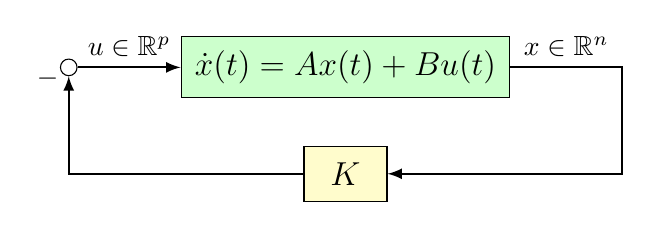
\begin{tikzpicture}[auto, >=latex]
    \node (input) [sum] {};
    \node (plant) [block, fill=green!20, font=\large, right of=input, node distance=10em] {$\dot{x}(t)  = A x(t) + B u(t)$};
    \node (output) [coord, right of=plant, node distance=10em] {};
    \node (controller) [block, font=\large, below of=plant, yshift=-1em] {$K$};

    \draw [connector] (plant) -- node [above] {$x \in \mathbb{R}^n$} (output) |- (controller);
    \draw [connector] (controller) -| node [pos=0.99] {$-$} (input);
    \draw [connector] (input) -- node [above] {$u \in \mathbb{R}^p$} (plant);
  \end{tikzpicture}
  \caption{Schematic of a full-state feedback system}
\end{figure}


\subsection{ Observer design}
The observer can be designed using a quadratic estimator known as the Kalman filter. This method is optimal if the errors in representing the state $x(t)$ and the measurements $y(t)$ are stochastic Gaussian processes. Such errors typically arise from inaccuracies in the model, external disturbances, and sensor noise.

A standard linear \textbf{observer} reconstructs a state estimate~$\hat x$, with dynamics given by
\begin{equation}
		\dot{\hat{x}}(t) = (A- L C) \hat{x}(t) + B u(t) + L y(t),
		\label{obslti}
\end{equation}
where the matrices $A,B$ and~$C$ are the same as those in the system~(\ref{lti1}), and $L$ is a matrix of gains chosen such that the state estimate converges quickly relative to the system's dynamics.

Using our linear model, we design an \textbf{optimal observer} (Kalman filter) to find~$L$.
We introduce two zero-mean Gaussian white noise processes, $w$ the process disturbance and $v$ the sensor noise, with respective covariance matrices $W$ and~$V$, into equations (\ref{lti1}) to obtain
\begin{align}
	\dot{x}(t) &= A x(t) + B u(t) + w(t),\\
	y(t) &= C x(t) + v(t). 
\end{align}
Then the covariance of the error in the state estimate is minimized (assuming the noise models are correct) by setting
\begin{equation}
	L = P C^T V^{-1},
\end{equation}
where $P \in \mathbb{R}^{n \times n}$ ($P>0$)  is a positive-definite symmetric matrix that solves another algebraic Riccati equation.
%\begin{equation}
%A {P} + P {A}^T - P {C}^T V^{-1} C P + W = 0.
%\end{equation}

The observer generates an estimate of the state from the physics model as represented by the state matrix, the inputs and outputs, and once combined to the feedback controller it forms a linear quadratic Gaussian compensator called LQG.

The LQG controller can stabilize any plant that is detectable and stabilizable, meaning that the actuators can \emph{control} and the sensors can \emph{observe} all unstable eigenmodes of $A$. The controller may not always be robust though, then robust control tools can attempt to improve the robustness of the closed-loop systems.

\begin{figure}[htbp]
\centering
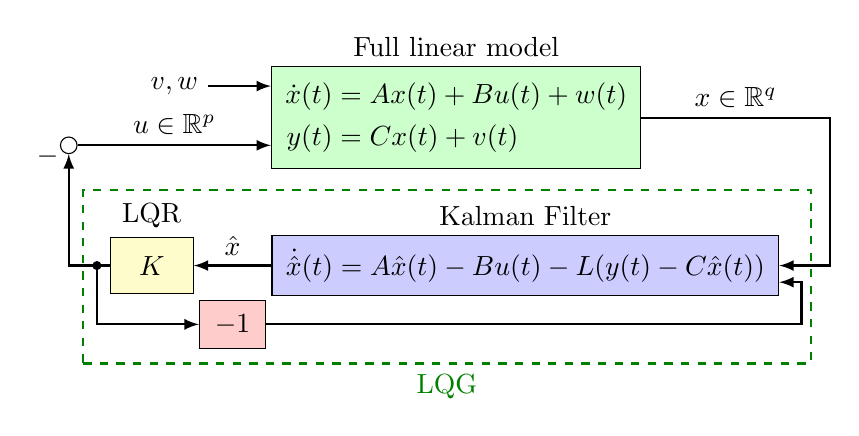
\begin{tikzpicture}[auto, >=latex]
    \node (input) [sum] {};
    \node (plant) [block, fill=green!20, right of=input, node distance=14em, yshift=1em, label=above:Full linear model] {$\begin{aligned} \dot{x}(t) &= A x(t) + B u(t) + w(t) \\ y(t) &= C x(t) + v(t) \end{aligned}$};
    \node (output) [coord, right of=plant, node distance=13.5em] {};
    \node (observer) [block, fill=blue!20, below of=plant, xshift=2.5em, yshift=-2.5em, label={[name=label_observer]above:{Kalman Filter}}] {$\dot{\hat x}(t) = A \hat{x}(t) - B u(t) - L (y(t) - C \hat{x}(t))$};
    \node (controller) [block, below of=plant, xshift=-11em, yshift=-2.5em, label={[name=label_controller]above:LQR}] {$K$};

    \draw [connector] (plant) -- node [above] {$x \in \mathbb{R}^q$} (output) |- (observer);
    \draw [connector] (observer) -- node [name=xr, above] {$\hat{x}$} (controller);
    \draw [connector] (controller) -| node [pos=0.99] {$-$} (input);
    \draw [connector] (input) -- node [name=u, above] {$u \in \mathbb{R}^p$} (input-|plant.west);
    
    \node (noise) [above=0em of u] {$v,w$};
    \draw [connector] (noise) -- (noise-|plant.west);
    
    \node (-1) [block, fill=red!20, below of=xr, minimum height=1.5em, minimum width=2.4em] {$-1$};
    \node (out) [junction, left=0.3em of controller] {};
    \node (in) [coord, right=0.8em of observer, yshift=-0.6em] {};
    \draw [connector] (out) |- (-1);
    \draw [connector] (-1) -| (in) -- (in-|observer.east);
    \node [draw, green!50!black, thick, dashed, fit=(observer) (controller) (-1) (label_observer) (label_controller) (out) (in), label={[green!50!black]below:LQG}, yshift=-0.2em] {};
\end{tikzpicture}
\caption{Schematic of an observer (Kalman filter) connected to a controller (LQR) to form a compensator (LQG)}
\end{figure}


%%%\subsection{Integrator, actuators saturation and anti-windup design} 
%%%
%%%We can split the feedback control theory into two main applications, one is disturbance rejection and the other one is reference tracking.
%%%
%%%If the primary goal is tracking a desired reference signal, then we want to minimize the steady state error between the output measurements ($y(t)$) and the corresponding desired values ($y_d$). One way to handle such issue is to use \textbf{integral action}.
%%%
%%%We thus introduce a new state variable~$z$ that is the integral of the error:
%%%\begin{equation}
%%%	\dot{z}(t) = y_{d} - y(t) = y_{d} - C x(t).
%%%	\label{integral01}
%%%\end{equation}
%%%The overall system (\ref{lti1}) can be then written as
%%%\begin{equation}
%%%\renewcommand\arraystretch{0.8}
%%%\frac{\partial}{\partial t} \begin{bmatrix}  x(t) \\ z(t) \end{bmatrix}
%%%  = { \begin{bmatrix} A  & 0 \\ -C & 0 \end{bmatrix} } \begin{bmatrix} x(t) \\ z(t) \end{bmatrix}
%%%  + \begin{bmatrix} B \\ 0 \end{bmatrix} u(t) + \begin{bmatrix} 0 \\ I \end{bmatrix} y_{d}
%%%\label{integral02}
%%%\end{equation}
%%%with a new feedback law designed as
%%%\begin{equation}
%%%u(t)  = u_d + K (x_d - x(t)) + K_I \!\!\int (y_d - y(t)) \, dt
%%%\end{equation}
%%%where $K$ is the optimal feedback gain defined through LQR and $K_I$  the optimal integral gain. Both of these gains are obtained by solving a continuous algebraic Riccati equation (CARE) with an extended state that includes the integrator defined in equation (\ref{integral01}).
%%%
%%%A drawback of integral control is that if any actuator value is limited to some range $u\in[u_\text{min},u_\text{max}]$ (as they are in most plasma experiments), then the integrator can accumulate error when the actuator is \emph{saturated}, resulting in poor transient performance, a phenomenon known as \textbf{integrator windup}.  
%%%
%%%We can avoid these effects by using a standard \textbf{anti-windup} technique (see, e.g., \cite{AandM, Lewis}), in which one feeds back the difference between the desired value of~$u$ and its actual (possibly saturated) value, as shown in the diagram in Figure~\ref{fig:model13}.  
%%%
%%%Figure~\ref{fig:model13} shows the schematic of the overall controller, combining the feedback law~(\ref{ltilqr}) with the observer law~(\ref{obslti}), the integrator~(\ref{integral01}) and the anti-windup approach described above. 
%%%
%%%\begin{figure*}
%%%\begin{tikzpicture}[x=0.75cm]
%%%		\node (r) {$y_{d}$};
%%%		\node[junction, right=1.5 of r] (r in) {};
%%%		\node[block, right=2 of r in] (F) {$F$};
%%%		\node[block, below=of F] (L) {Observer};
%%%		\node[sum, right=of L] (sum feedback) {};
%%%		\node[block, right=0.9 of sum feedback] (K) {$K$};
%%%		\node[sum, right=5 of F, yshift=3] (sum inputs) {};
%%%		\node[junction, right=1 of sum inputs] (before sat) {};
%%%		\node[block, right=0.5 of before sat] (sat) {
%%%			\begin{tikzpicture}
%%%				\draw[very thin] (-.4,0) -- (.4,0) (0,-.25) -- (0,.25);
%%%				\draw[very thick] (-.4,-.2) -- (-.2,-.2) -- (.2,.2) -- (.4,.2);
%%%			\end{tikzpicture}
%%%		};
%%%		\node[junction, right=0.5 of sat] (after sat) {};
%%%		\node[block, right=1.5 of after sat] (P) {Plant};
%%%		\node[junction, right=0.7 of P] (P out) {};
%%%		\node[right=0.7 of P out] (y) {$y$};
%%%		\node[junction, left=1 of L, yshift=3] (y in) {};
%%%		\node[coord, left=1 of L, yshift=-3] (sub y in) {};
%%%		\node[coord, label=left:$y$, left=2.4 of y in] (y input) {};
%%%		\node[block, above=of F] (Ki) {$K_I$};
%%%		\node[sum] (sum lqi) at (Ki -| y in) {};
%%%		\node[sum, right=of Ki] (AW out) {};
%%%		\node[block, right=0.9 of AW out] (integrator) {$\int$};
%%%		\node[sum, above=0.5 of sat] (sum AW) {};
%%%		\node[block, above=0.5 of sum AW] (AW) {AW};
%%%		
%%%		\draw[connector] (r) to (r in) to (F);
%%%		\draw[connector] (F.east |- sum inputs) to node [above] {$u_{d}$} (sum inputs);
%%%		\draw[connector] (F)[yshift=-12] -| node [right, near end] {$x_{d}$} (sum feedback);
%%%		\draw[connector] (sum feedback) to (K);
%%%		\draw[connector] (K) -| (sum inputs);
%%%		\draw[connector] (sum inputs) to (before sat) to (sat);
%%%		\draw[connector] (sat) to (after sat) to ++(down:2.6) -| (sub y in) to (sub y in -| L.west);
%%%		\draw[connector] (after sat) to node [above, pos=0.7] {$u$} (P);
%%%		\draw[connector] (P) to (P out) to (y);
%%%		\draw[connector] (P out) -- ++(down:3.5) -| (y input) to (y in) to (y in -| L.west);
%%%		\draw[connector] (L) to node [above] {$\hat x$} node [below, very near end] {$-$} (sum feedback);
%%%		\draw[connector] (r in) |- (sum lqi);
%%%		\draw[connector] (y in) to node [right, pos=0.95] {$-$} (sum lqi);
%%%		\draw[connector] (sum lqi) to (Ki);
%%%		\draw[connector] (Ki) to (AW out);
%%%		\draw[connector] (AW out) to (integrator);
%%%		\draw[connector] (integrator) -| (sum inputs);
%%%		\draw[connector] (before sat) |- node [below, very near end] {$-$} (sum AW);
%%%		\draw[connector] (after sat) |- (sum AW);
%%%		\draw[connector] (sum AW) to (AW);
%%%		\draw[connector] (AW) to ++(up:0.6) -| (AW out);
%%%		
%%%		\draw[green!50!black, ultra thick] (1.4,-2.8) rectangle (15.5,3.1);
%%%		\node[green!50!black, anchor=south, font=\large\bfseries] at (8.4,3.1) {Controller};
%%%	\end{tikzpicture}
%%%
%%%\caption{Global schematic of the controller that combine a feedforward ($F$), a LQR ($K$), an observer, an integrator $(K_I)$ and an anti-windup (AW).}
%%%\label{fig:model13}
%%%\end{figure*}
%%%


%\section{Robust control tools}
%
%Although the closed-loop systems we obtain using the methods described above are stable in theory, multiple factors could make them unstable in practice, or adversely affect their performance.
%The models on which they are based might be inaccurate, some elements of the dynamics might be missing, or some of the parameters might be off.
%All these inaccuracies are referred as \emph{model uncertainty}.
%Fortunately it is possible to precisely describe this uncertainty, put proper bounds on it, and guarantee that our closed-loop systems stay stable and meet all performance specifications in spite of it. More details can be found in~\cite{SandP}.
%
%In this section, we show how to represent system uncertainty resulting from parameter uncertainty and we give conditions for robust stability and performance.
%We describe robustness analysis for systems with a single input and a single output (SISO) first, then for systems with multiple inputs and multiple outputs (MIMO) which will be our practical case in this disertation.
%
%\subsection{Uncertainty and robustness for SISO systems}
%
%Let $G$ be the model representing the system that we want to control.
%We call it the \textbf{nominal model} and we use it to design a controller.
%Because of various uncertainties, or the desire to keep model complexity low (e.g., linearization, model reduction), it is possible that $G$ is not a very accurate representation of the actual underlying system and that the controller we designed would either be unstable or have poor performance when applied to the actual system.
%The actual system can be seen as a perturbed version $G_p$ of our nominal model $G$.
%However, we do not know exactly where $G_p$ lies compared to $G$ but we can be conservative and make our controller robust to any bounded perturbation with sufficiently large bounds to make sure that the set $\Pi$ of all perturbed models contains $G_p$.
%We say that robust stability (resp. performance) is obtained when all plants in $\Pi$ are stable (resp. performant).
%
%One way to put bounds on the perturbations is to rely on parametric uncertainty.
%It is often the case that instead of a precise value, we only know a range of possible values for some parameters in our systems.
%We can use this structured information to compute analytical bounds on the perturbations of the model.
%
%To greatly simplify the analysis while being strictly conservative about stability and performance, we can use a \emph{norm-bounded} description of uncertainty where $\Pi$ is allowed to contain $\mathcal{H}_\infty$ norm-bounded perturbations of our nominal model $G$.
%There are different ways to integrate this uncertainty into a model but one can get intuition on which one to use by observing the patterns obtained by superimposing the Nyquist plots of many perturbed models.
%Here we will only describe multiplicative uncertainty which is one of the most common.
%The perturbed model can be written as
%\begin{equation} \label{eq:multiplicative}
%	G_p = G (1 + \Delta W),
%\end{equation}
%where $W$ is a weighting transfer function, and $\Delta$ is a transfer function satisfying $\|\Delta\|_\infty < 1$.
%A block diagram of the perturbed plant is shown in Figure~\ref{fig:example_multiplicative}.
%
%\begin{figure}[htbp]
%	\centering
%	\begin{tikzpicture}
%		\node (u) {$u$};
%		\node[junction, right=0.5 of u] (in) {};
%		\node[coordinate, right=1 of in] (below Delta) {};
%		\node[block, above=0.5 of below Delta] (Delta) {$\Delta$};
%		\node[coordinate, right=1.7 of below Delta] (below W) {};
%		\node[block, above=0.5 of below W] (W) {$W$};
%		\node[sum, right=0.9 of below W] (sum) {};
%		\node[block, right=0.5 of sum] (G) {$G$};
%		\node[right=0.5 of G] (y) {$y$};
%		
%		\draw[connector] (u) to (in) to (sum);
%		\draw[connector] (sum) to (G);
%		\draw[connector] (in) |- (Delta);
%		\draw[connector] (Delta) to (W);
%		\draw[connector] (W) -| (sum);
%		\draw[connector] (G) to (y);
%	\end{tikzpicture}
%	\caption{Perturbed model $G_p = G (1 + \Delta W)$}
%	\label{fig:example_multiplicative}
%\end{figure}
%
%To find $W$, we first observe that $\Delta W = {G_p}/{G} - 1$.
%Thus we can superimpose the Bode plots of ${G_p}/{G} - 1$ for many perturbed plants and choose a low-order upper bound which will be our $W$.
%
%Next we want to check robust stability. Using the Nyquist criterion we require that for any perturbed model $G_p$, the corresponding loop gain $L_p$ should not encircle the -1 point. 
%This translates to the condition
%\begin{equation}
%	\| W T \|_\infty < 1,
%\end{equation}
%where $T = \frac{L}{1 + L}$ is the complementary sensitivity function.
%
%Finally we want to check robust performance. We simply require that for any perturbed model $G_p$, a certain performance criterion is satisfied.
%The performance criterion is a set of constraints on the sensitivity function $S = \frac{1}{1 + L}$.
%For instance one can specify a minimum bandwidth, which relates to the speed of the response but also the sensitivity to noise, or an upper bound on peaks values which relates to stability margins.
%These specifications are encoded in a weight $W_P$ (where $P$ stands for \emph{performance}, whereas $p$ stands for \emph{perturbed}).
%The condition translates to
%\begin{equation}
%	\max_\omega(| W_P S | + | W T |) < 1.
%\end{equation}
%
%\subsection{Robust Stability and performance analysis for MIMO systems}
%
%The robustness analysis for multiple inputs and multiple outputs (MIMO) systems is very similar but slightly more complex than for SISO systems. In a MIMO system, each input may influence any or all outputs and each output may be influenced by any or all inputs.
%
%A first complication of working with a MIMO system is that all transfer functions are now matrices and as such, multiplication is no longer commutative.
%One consequence is that common SISO transfer functions like the loop gain, the sensitivity, and the complementary sensitivity exist in two variants: input or output depending of the order of multiplication.
%Also, looking at one bode plot per input-output pair can quickly become unwieldy, so instead it is often convenient to look at Bode plots of the singular values of a transfer function matrix.
%Furthermore, upper bounds for robustness and performance are often expressed in terms of the largest singular value $\bar\sigma(H)$ for a transfer function matrix $H$.
%
%% Nominal Stability
%
%Before introducing uncertainty, the first step is to verify that the closed-loop nominal system is stable and define performance specifications.
%For the nominal stability, one can inspect the open loop poles and the Nyquist plot of the system and use the Nyquist criterion to conclude.
%
%% Nominal Performance
%
%Performance is a trade-off between getting a fast response (for instance while tracking the reference signal for a tracking problem) and making sure that measurement noise and other disturbances are not amplified too much by the feedback loop.
%Fortunately, these disturbances enter the system at different points in the loop and sometimes at different frequencies than the reference signal.
%
%We define nominal performance by choosing upper bounds on the transfer functions from these disturbance inputs (sometimes called exogenous outputs) to various points in the feedback loop, typically to the output $y$ and to the input $u$.
%There are two important aspects to consider when choosing the bounds.
%The \emph{static} aspect is given by the \emph{peaks} (maximum values) which are related to the quality of the response.
%The \emph{dynamic} aspect is given by the \emph{bandwidth frequency} which is related to the speed of the response.
%In general, a large bandwidth means better performance since high frequency signals are more easily passed on to the outputs, so the rise time is improved, but it also indicates a system which is sensitive to noise and model uncertainties.
%
%In a MIMO system, typical transfer functions of interest include the input and output sensitivities $S_i$ and $S_o$, the input and output complementary sensitivities $T_i$ and $T_o$, and combinations of the sensitivities with the system $G$ and the controller $K$.
%
%% Uncertainty modeling
%
%As in the previous section, we introduce parametric uncertainty which we translate into multiplicative uncertainty.
%In this example, we use right multiplicative uncertainty, as opposed to left (or inverse) multiplicative uncertainty, since the order of multiplications matters.
%The perturbed plant $G_p$ can be written as
%\begin{equation} \label{eq:multiplicative_MIMO}
%	G_p = G (I + W_1 \Delta W_2),
%\end{equation}
%where $W_1$ and $W_2$ are weighting transfer function matrices, and $\Delta$ satisfies $\|\Delta\|_\infty < 1$.
%For simplicity, $W_1$ is often taken to be the identity matrix.
%A block diagram of the perturbed plant is shown on Figure~\ref{fig:example_perturbed_MIMO}.
%
%\begin{figure}[htbp]
%	\centering
%	\begin{tikzpicture}
%		\node (u) {$u$};
%		\node[junction, right=0.5 of u] (in) {};
%		\node[coordinate, right=1 of in] (below W2) {};
%		\node[block, above=0.5 of below W2] (W2) {$W_2$};
%		\node[coordinate, right=1.7 of below W2] (below Delta) {};
%		\node[block, above=0.5 of below Delta] (Delta) {$\Delta$};
%		\node[coordinate, right=1.7 of below Delta] (below W1) {};
%		\node[block, above=0.5 of below W1] (W1) {$W_1$};
%		\node[sum, right=0.9 of below W1] (sum) {};
%		\node[block, right=0.5 of sum] (G) {$G$};
%		\node[right=0.5 of G] (y) {$y$};
%		
%		\draw[connector] (u) to (in) to (sum);
%		\draw[connector] (sum) to (G);
%		\draw[connector] (in) |- (W2);
%		\draw[connector] (W2) to (Delta);
%		\draw[connector] (Delta) to (W1);
%		\draw[connector] (W1) -| (sum);
%		\draw[connector] (G) to (y);
%	\end{tikzpicture}
%
%	\caption{Perturbed model $G_p = G (I + W_1 \Delta W_2)$}
%	\label{fig:example_perturbed_MIMO}
%\end{figure}
%
%To find $W_2$ (we assume that $W_1 = I$), we proceed exactly as in the previous section, except that $W_2$, $G$ and $G_p$ are now matrices so we must find upper bounds for each element of the $G^{-1}{G_p} - I$ matrix.
%
%% Robust stability
%
%Now equipped with a mathematical description of our perturbed system, we can address robust stability.
%For stability we only need to consider the feedback loop. Exogenous inputs are only relevant for performance.
%It is always possible using block diagram algebra to rearrange a system to put it in the $M \Delta$ configuration as shown in \ref{fig:example_diagram_perturb}.
%Once we know $M$, the condition for robust stability is simply:
%\begin{equation}
%	\| M \|_\infty < 1.
%\end{equation}
%
%\begin{figure}
%	\centering
%	\begin{tikzpicture}
%		\node[font=\large\bfseries] at (-0.25,1.25) {a)};
%		\path (0,1.25) -- ++(down:2.75);
%
%		\node[sum] (sum) {};
%		\node[junction, right=0.5 of sum] (in) {};
%		\node[coordinate, right=of in] (below W2) {};
%		\node[block, above=0.4 of below W2] (W2) {$W_2$};
%		\node[coordinate, right=2 of below W2] (below Delta) {};
%		\node[block, above=0.4 of below Delta] (Delta) {$\Delta$};
%		\node[coordinate, right=2 of below Delta] (below W1) {};
%		\node[block, above=0.4 of below W1] (W1) {$W_1$};
%		\node[sum, right=of below W1] (out) {};
%		\node[block, right=0.5 of out] (G) {$G$};
%		\node[coordinate, right=0.5 of G] (end) {};
%		\node[coordinate] (above K) at ($(sum)!0.5!(end)$) {};
%		\node[block, below=0.6 of above K] (K) {$K$};
%		
%		\draw[connector] (sum) to (in) to (below W2) to (below Delta) to (below W1) to (out) to (G);
%		\draw[connector] (G) to (end) |- (K);
%		\draw[connector] (K) -| node[right, pos=0.98] {$\scriptstyle -$} (sum);
%		
%		\draw[connector] (in) |- (W2);
%		\draw[connector] (W2) to node[above] {$u_\Delta$} (Delta);
%		\draw[connector] (Delta) to node[above] {$y_\Delta$} (W1);
%		\draw[connector] (W1) -| (out);
%	\end{tikzpicture}
%	\begin{tikzpicture}
%		\node[font=\large\bfseries] at (-2,0.5) {b)};
%		\path (0,0.5) -- ++(down:2.75);
%		
%		\node[block] (Delta) {$\Delta$};
%		\node[block, below=0.5 of Delta] (M) {$M$};
%		
%		\node[coord, right=0.6 of M] (right) {};
%		\node[coord, left=0.6 of M] (left) {};
%		
%		\draw[connector] (M.east) to (right |- M) to node[right] {$y_\Delta$} (right |- Delta) to (Delta);
%		\draw[connector] (Delta) to (left |- Delta) to node[left] {$u_\Delta$} (left |- M) to (M);
%	\end{tikzpicture}
%
%	\caption{Block diagrams of the loop of the perturbed closed-loop system stripped of all exogenous inputs and outputs. \textbf{a)} Expanded system. \textbf{d)} $M \Delta$ structure for robust stability analysis.}
%	\label{fig:example_diagram_perturb}
%\end{figure}
%
%
%However there is no simple analytical method for asserting robust performance for MIMO systems so we will have to resort to numerical methods \emph{\`a la Monte Carlo}.
%One simple way to test for robust performance is to generate many perturbed plants and check that each one of them satisfies the performance specifications by superimposing the Bode plots of the singular values of the perturbed plants. More details on the topic can be found in \cite{SandP}


\chapter{Hasegawa-Wakatani problem}
\label{haswak}
%The methodology that we would like to emphasize and which has been used throughout this work is the \textbf{model-based feedback control design approach}. It combines tools described in Chapters \ref{chapitre2} and its main steps can be described as follows: \\
%%
%\begin{itemize}
%\item \textbf{Step 1:}  Find an equilibrium and linearize the input-output system around it.
%\item \textbf{Step 2:}  Build a reduced-order model (ROM) of the linear system.
%\item \textbf{Step 3:}  Design an observer-based feedback controller using the ROM.
%\item \textbf{Step 4:}  Apply the feedback controller to the full linear and nonlinear system.\\
%\end{itemize}
%%

Here, we apply the methods discussed in the previous chapter to a problem in plasma physics known as
the Hasegawa-Wakatani (HW) problem \cite{Hasegawa1,Hasegawa2}.
\section{Modified Hasegawa-Wakatani modeling}

Drift wave instabilities are an important type of instabilities of fluid plasmas. They occur when a non-uniform density plasma is maintained in an equilibrium by a strong magnetic field. Drift wave instabilities can transport the thermal energy of the plasma as it expands across a magnetic field. This undesirable transport leads to energy and confinement loss that can lead to a plasma termination. Our control objective is therefore to stabilize these drift waves instabilities.

The HW model which couples plasma density and electrostatic potential through an approximation of the physics of parallel electron motion, is a simple model that describes resistive drift wave turbulence. It was developed to investigate the observed anomalous edge transport due to collisional drift waves~\cite{Horton}.

\begin{figure}[htbp]
\centering
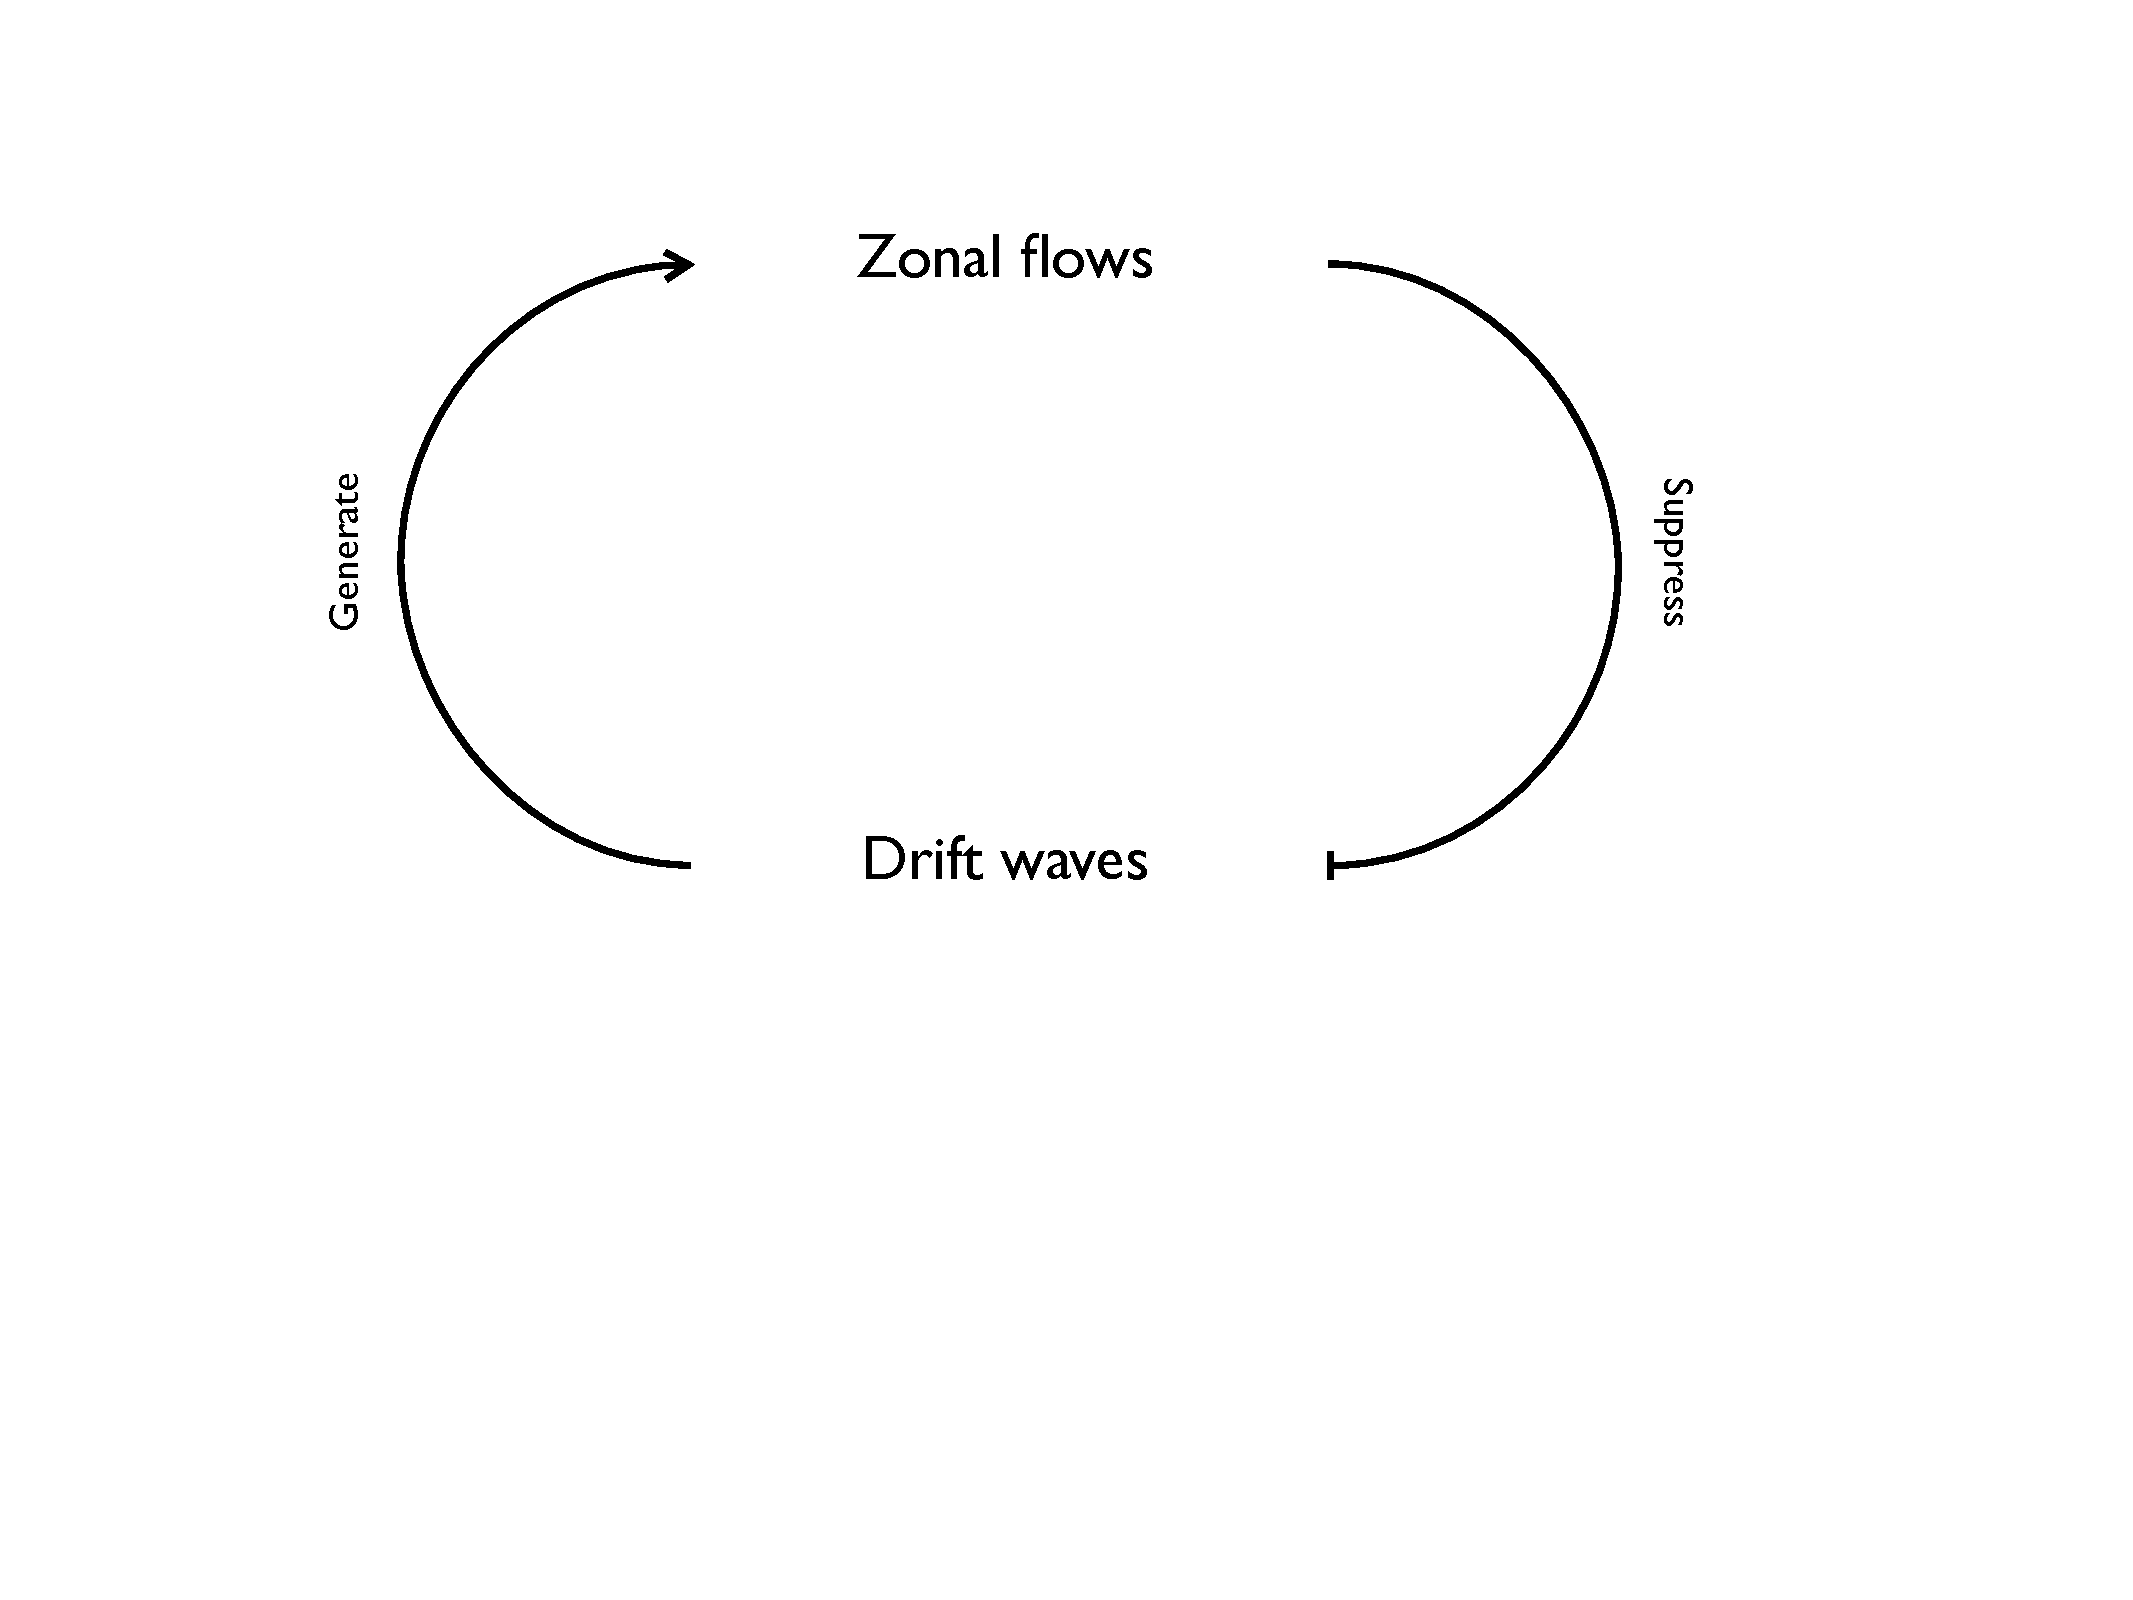
\includegraphics [width=0.7\linewidth]{rel} 
\caption{Schematic of drift waves / zonal flow coupling}
\label{rel}
\end{figure}

Due to nonlinearity, drift waves can self-consistently generate zonal flows, which in turn play a key role in the regulation of these drift-wave instabilities and thus in the suppression of the anomalous transport, see Figure~{\ref{rel}}. The modified HW model \cite{Hasegawa1,Hasegawa2} capture this coupled mechanism in the following equations
\begin{subequations}
\label{HW1}
\begin{align}
	\frac{\partial \zeta}{\partial t}  + \{\varphi , \zeta \} &= \alpha ({\varphi}-{n}) - \mu \Delta^2 \zeta \label{MHWeqs1}	, \\	
	\frac{\partial n}{\partial t}  + \{\varphi , n\} &=  \alpha ({\varphi}-{n}) -\kappa \frac{\partial \varphi}{\partial y}- \mu \Delta^2 n,
\label{HW2}	
\end{align}
\end{subequations}
where $n$ is the density and $\varphi$ is the electrostatic potential with $\zeta = \Delta \varphi$, $\Delta = \partial ^2 / \partial x^2+ \partial ^2 / \partial y^2$ is the 2D Laplacian, $\{a,b\} \equiv  \left( \partial a /\partial x  \right)\left( \partial b /\partial y \right)  -\left( \partial a /\partial y  \right)\left( \partial b /\partial x \right) $ is the Poisson bracket, $\mu$ is the dissipation coefficient, the background density $n_0$ is assumed to have a fixed exponential profile, so that the background density gradient  $\kappa \equiv  \left( \partial  /\partial x \right) \ln n_0$ is assumed constant, $\alpha $ is the adiabaticity operator.

In this 2D spatio-temporal evolution of the density $n$ and the ion vorticity $\zeta$, $\alpha$, $\mu$, and $\kappa$ are considered to be time- and space-invariant constants.

We analyze drift waves in the simplest possible configuration involving a non-uniform plasma called \emph{plane plasma slab}. In this configuration, there is a plasma with non-uniform density $n$ and pressure $p$ maintained in equilibrium by a strong magnetic field $B_0$ as shown in Figure~\ref{waka1}

\begin{figure}[htbp]
\centering
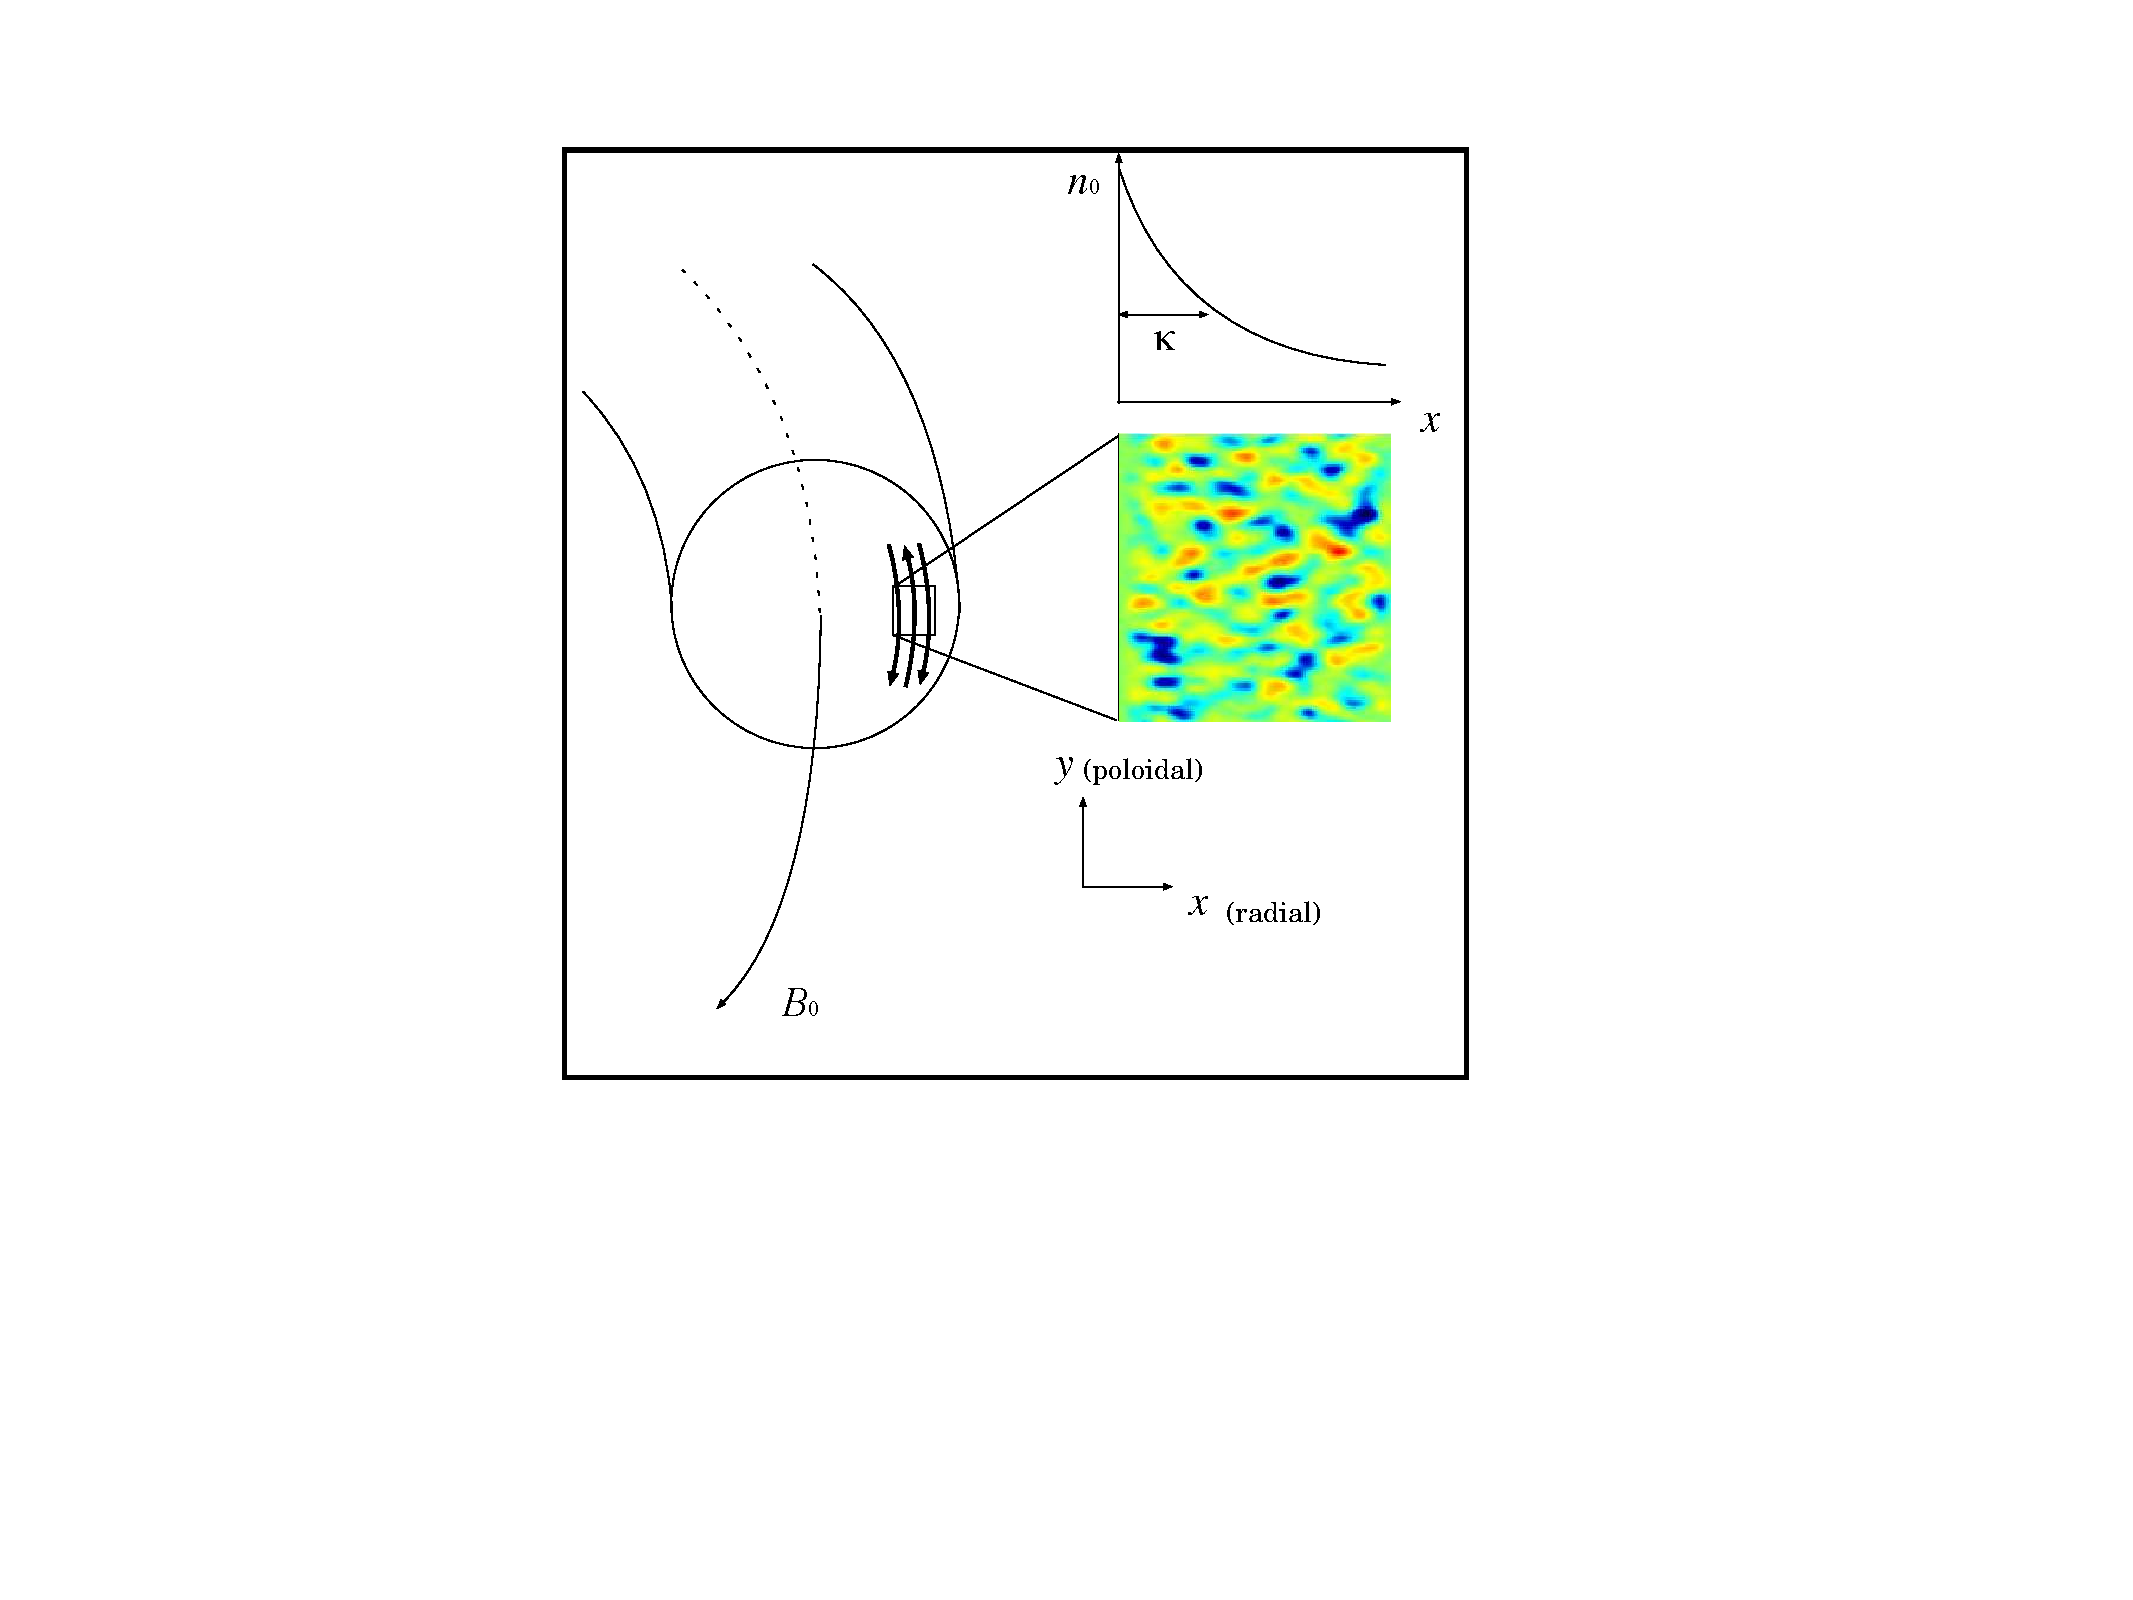
\includegraphics[width= 0.6\linewidth]{waka1}
\caption{Schematic of drift wave modeling location }
\label{waka1}
\end{figure}

Parallel electron motion is a key element for generating, stabilizing, and destabilizing zonal flow. However, for computational reasons, HW model is usually studied as a 2D model \cite{Smolyakov, Numata}. Originally, the parallel dissipation operator $-D_\parallel \nabla_\parallel^2$ was just replaced by a constant $\alpha$ defined above (essentially assuming the presence of a single, dominant, nonzero parallel wave number $k_\parallel$).  However, that approximation is incorrect for zonal flows, for which $k_\parallel = 0$.  

Therefore, in the modified Hasegawa-Wakatani model (MHW), the parallel term is taken to vanish for the zonal modes~\cite{Smolyakov}. The modified equations are
\begin{subequations}
\label{MHW1a}
\begin{align}
	\frac{\partial \zeta}{\partial t}  + \{\varphi , \zeta \} &= \alpha (\tilde{\varphi}-\tilde{n}) - \mu \Delta^2 \zeta \label{MHW1aa}	, \\	
	\frac{\partial n}{\partial t}  + \{\varphi , n\} &=  \alpha (\tilde{\varphi}-\tilde{n}) -\kappa \frac{\partial \varphi}{\partial y}- \mu \Delta^2 n,
\label{MHW1bb}	
\end{align}
\end{subequations}
%
where zonal and nonzonal components of a variable $f$ are defined as
\begin{subequations}
\begin{align}
\mbox{zonal:} \quad  \langle f  \rangle &\equiv \frac{1}{L_y} \int fdy, \\
 \mbox{nonzonal:} \quad   \tilde{f}  &\equiv f - \langle f  \rangle,
\end{align}
\end{subequations}
where $L_y$ is the periodicity length in $y$. Since we are considering the study in a plasma slab, periodic boundary conditions are used for simplicity.

Figure \ref{coupling} shows a simulation of this MHW model (\ref{MHW1a}) where the transition of both ion vorticity and density fluctuation from a horizontally uniform state (drift waves) to an almost  vertically uniform state (zonal~flow) is highlighted;  the model modification helps indeed simulating the complex coupling between drift waves and zonal flow. 
\begin{figure}[htb]
\centering
  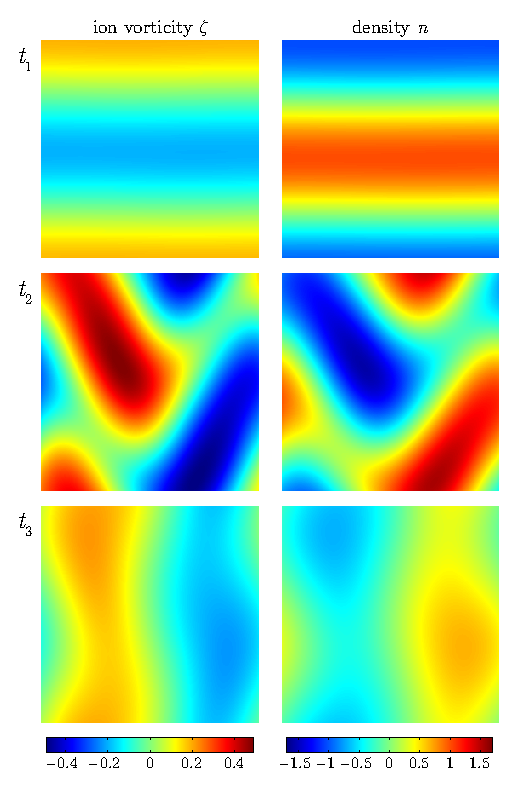
\includegraphics{video}
  \caption{Ion vorticity and density fluctuation (in color) of the full non linear MHW equations at three successive times.}
\label{coupling}
\end{figure}

\section{Results on model reduction}

To be able to apply model reduction, we need to linearize the non-linear system around an equilibrium to obtain a LTI system that can then be reduced.

We choose an unstable equilibrium point for (\ref{MHW1a}) which is ($\phi_0$ = 0, $\zeta_0$ = 0, $n_0=0$).
The linearization about this equilibrium is
\begin{subequations}
\begin{align}
\frac{\partial \zeta}{\partial t}  &= \alpha (\tilde{\varphi}-\tilde{n}) - \mu \Delta^2 \zeta, \label{eq:HW_lin_a} \\
\frac{\partial n}{\partial t}   &= \alpha (\tilde{\varphi}- \tilde{n}) -\kappa \frac{\partial \varphi}{\partial y}- \mu \Delta^2 n. \label{eq:HW_lin_b}
\end{align}
\end{subequations}
The equations can then be formatted in a matrix notation as
%
\begin{equation}
	\renewcommand\arraystretch{0.8}
	\frac{d}{dt} \begin{pmatrix} \zeta \\ n \end{pmatrix}
	= A \begin{pmatrix} \zeta \\ n \end{pmatrix}
	= \begin{pmatrix}
		\alpha \Delta^{-1} - \mu \Delta^2 & -\alpha \\
		\alpha \Delta^{-1} - \kappa \frac{\partial}{\partial y} \Delta^{-1} & -\alpha - \mu \Delta^2
	\end{pmatrix} \begin{pmatrix} \zeta \\ n \end{pmatrix}.
	\label{mat22}
\end{equation}

A linear forcing is introduced into this equation to indirectly act as a controlled input, allowing us to put the system in a standard state-space realization form so as to apply the model-based feedback control methodology.
An additional external electrostatic potential causing this linear forcing is used as the actual controlled input.
It can be thought of as a probe inside the tokamak, although in practice no probe can withstand the extreme temperatures found inside the chamber of a tokamak. The total electrostatic potential can be written as
%
\begin{equation}
	\varphi_{\rm total} = \varphi_{\rm int} + \varphi_{\rm ext},
\end{equation}
%
where $\varphi_{\rm int}$ is the internal potential, $\varphi_{\rm ext} = \Phi u$ is the external potential added as the control input, $u$ is a scalar, and $\Phi$ is a given column vector that specifies the external field's spatial distribution.
This field is localized in the middle of the square plate and it is determined by the function $\Phi(r) = 2 \left(1-r^2/\gamma^2\right) \exp \left(-r^2/\gamma^2\right)$ where $r^2 =\left(x- L_x/2\right)^2 +\left(y- L_y/2\right)^2 $ and $\gamma = 5$ is a given parameter.

Introducing this actuator into equations (\ref{eq:HW_lin_a}--\ref{eq:HW_lin_b}) yields the following controlled linearized Modified Hasegawa-Wakatani equations:
\begin{subequations}
\begin{align}
	\frac{\partial}{\partial t} \zeta &= \alpha (\tilde{\varphi}-\tilde{n}) +\alpha \tilde{\varphi}_{ext} - \mu \Delta^2 \zeta, \\
	\frac{\partial}{\partial t} n  &= \alpha (\tilde{\varphi}- \tilde{n}) +\alpha \tilde{\varphi}_{ext} -\kappa \frac{\partial \varphi}{\partial y}-\kappa \frac{\partial \varphi_{ext}}{\partial y}- \mu \Delta^2 n.
\end{align}
\end{subequations}
The system can then be rewritten in a state space realization form
%
\begin{equation}
	\frac{\partial}{\partial t} {\left( \begin{matrix} {\zeta} \\ {n} \end{matrix} \right)} =      A {\left( \begin{matrix} {\zeta} \\ {n} \end{matrix} \right)} + B u, 
\label{sy}
\end{equation}
where $A$ is already defined in (\ref{mat22})  and
%
\begin{align}
\label{init}
	B &= {\left( \begin{matrix} {\alpha \tilde{\Phi}} \\ {\alpha \tilde{\Phi} - \kappa \partial_y \Phi} \end{matrix} \right)} .
\end{align}

We are going to numerically study three cases obtained by using a different density gradient $\kappa$ parameter while keeping the $\alpha$ and $\mu$ parameters fixed. We obtain three different $A$ matrices, one for each case, with different numbers of right half plane (unstable) poles summarized in Table~\ref{Tabparameter1}.
Figure~\ref{eigcase} illustrates the poles obtained for the first case of Table~\ref{Tabparameter1}.


\begin{table}[htbp]
	\centering
	\caption{Summary of the parameters and number of unstable poles for the three cases studied.
		Parameters $\alpha$ and $\mu$ are fixed, only $\kappa$ varies.}
	\label{Tabparameter1}
	\begin{tabular}{ccccc} \\
		Case & \makebox[2.5em]{$\kappa$} & \makebox[2.5em]{$\alpha$}  & \makebox[2.5em]{$\mu$} & \# of RHP poles \\ \hline
		1 &0.20 &0.1   & 0.2 & 2  \\
		2 & 0.25&  0.1  & 0.2 & 4 \\
		3 & 0.28&   0.1 & 0.2 & 8  \\
	\end{tabular}
\end{table}

\begin{figure}[htbp]
	\centering
	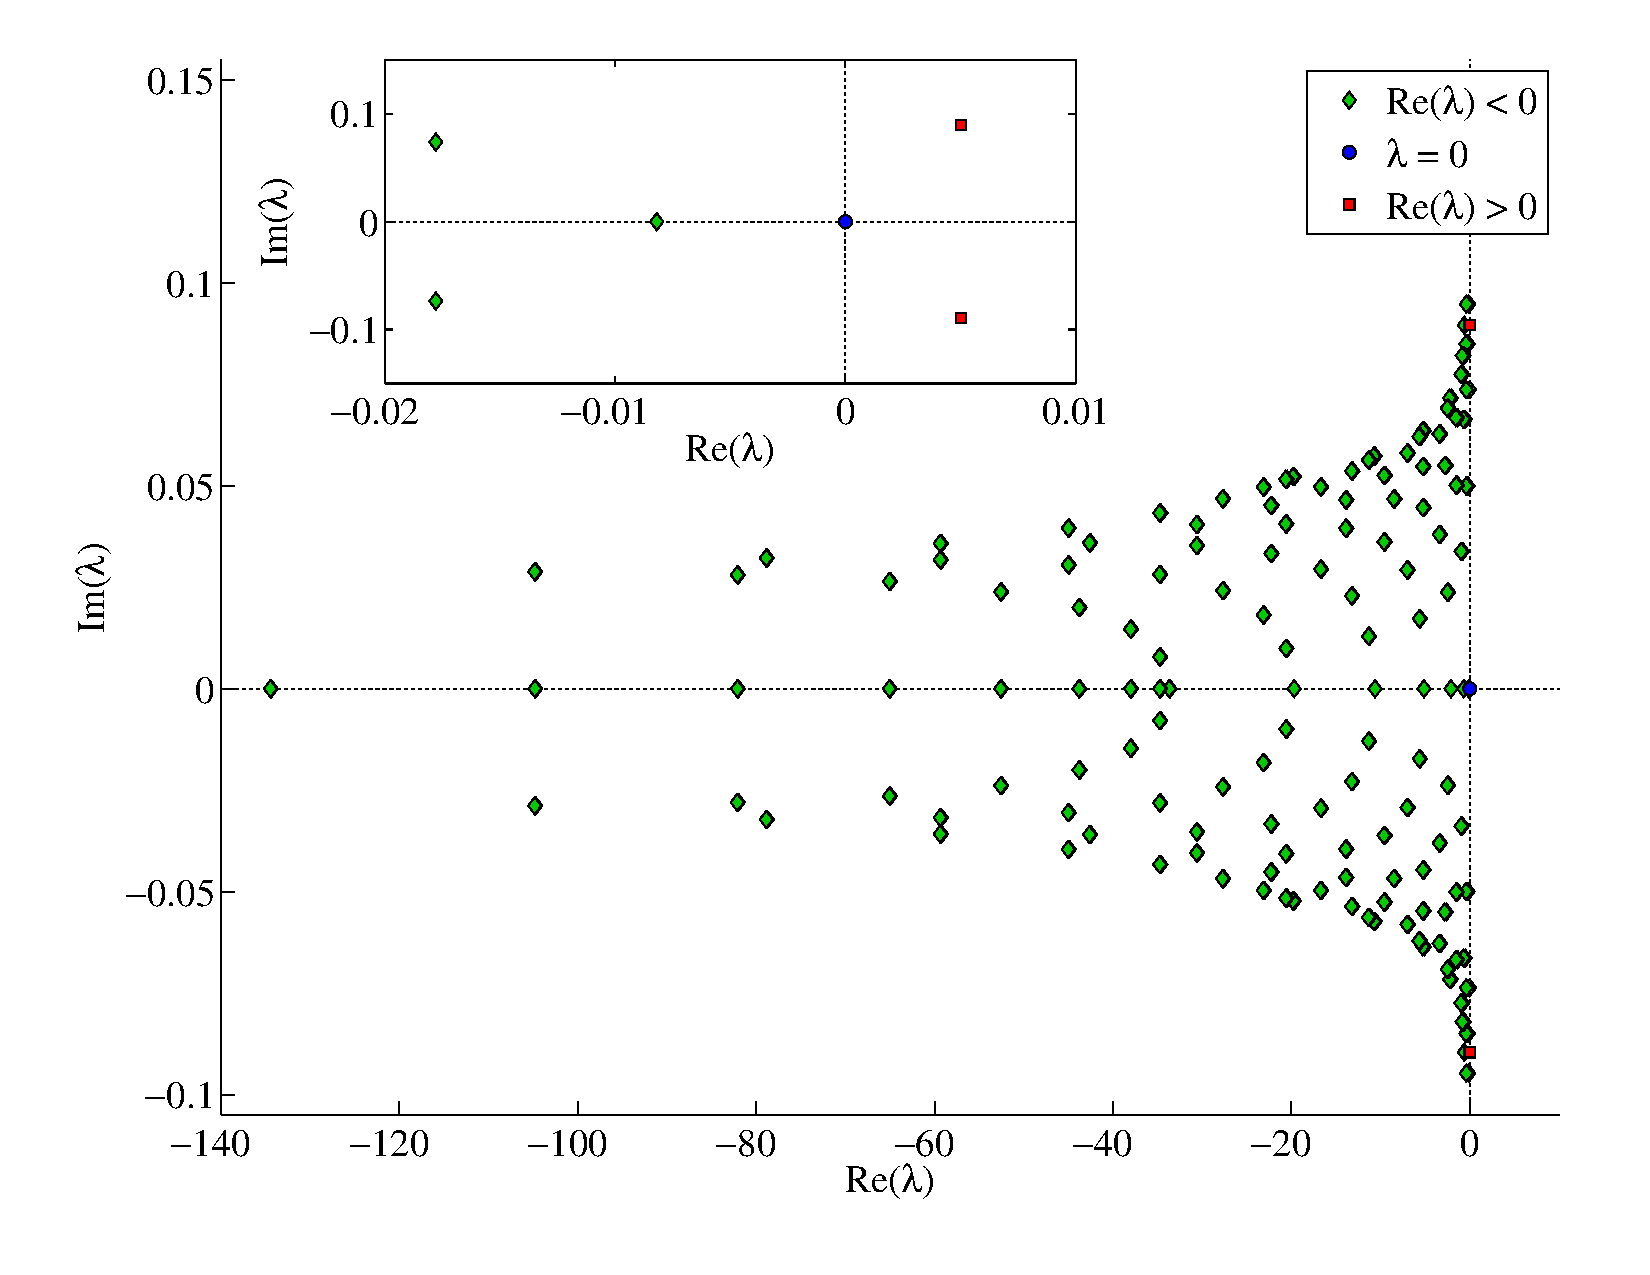
\includegraphics [width=0.7\linewidth]{case1a} 
	\caption{Representation of the poles of system (\ref{sy}) with $\kappa=0.2$ resulting in 2 right half plane (unstable) eigenvalues (Case \#1)}
	\label{eigcase}
\end{figure}

Once the balanced truncation is applied, the error between the original and the reduced-order model is calculated and compared to the theoretical bounds and to errors obtained by applying two other model reduction techniques seen in Chapter~\ref{chapitre2}: POD and BPOD. The results are presented in Figure~\ref{errorBT}.
As expected, the balanced truncation method is the one that gives the best approximation (least error) to the original model.
In addition, Figure~\ref{errorBT} allows us to decide where to truncate the model and how many modes to keep, for instance, in Case \#3 (with 8 unstable poles), the stable subsystem exhibits a truncation error of approximately $10^{-5}$ using only 12 modes. 

\begin{figure}[htbp]
	\centering
	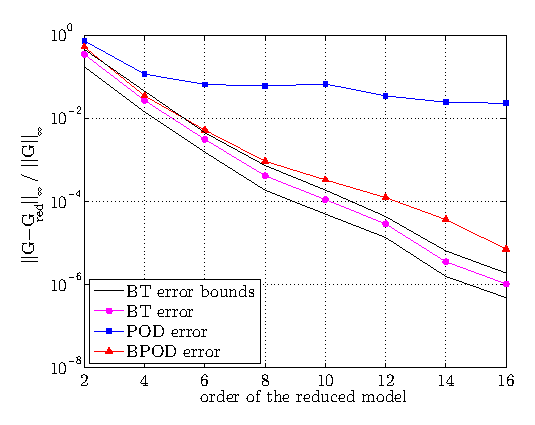
\includegraphics[width=0.7\linewidth]{error}
	\caption{Relative error $||G-G_\text{red.}||_{\infty} / ||G||_{\infty} $ for balanced truncation ($\bigcirc$), balanced POD ($\triangle$), POD ($\square$), and upper and lower bound for the model reduction scheme. }
	\label{errorBT}
\end{figure}

Table~\ref{Tabreduced2} shows the dimensions of the reduced order model obtained using balanced truncation for each case. We can see that in all three case the dimensionality has been significantly reduced.

The original 512 dimensions come from the fact that we are numerically solving the problem using a two-dimensional slab geometry with a grid size of $16 \times 16 = 256$ points for both the ion vorticity and the density (full state of dimension $256 \times 2 = 512$).

\begin{table}[htbp]
	\centering
	\caption{Summary of the effect of model reduction on the dimensionality of the system.
		$r$ is the dimension of the stable reduced  subsystem.}
	\label{Tabreduced2}
	\begin{tabular}{ccccc} \\[-0.5em]
		Case & Original dim. & \# of RHP poles &  \makebox[2em]{$r$} & Final dim. \\ \hline
		1 & 512 & 2 &  4 &  6  \\
		2 & 512 & 4 &  6 & 10 \\  
		3 & 512 & 8 &12 & 20 \\
	\end{tabular}
\end{table}


\section{Results on control and stability}

Once the reduced order models for all three cases are obtained, we carry on to the next step which is the design of the reduced order observer-based feedback controller.

For Case \#2, a 10 mode reduced-order model with 4 unstable and 6 stable modes is used to design the Kalman Filter which produces an optimal estimate of the density fluctuation and ion vorticity fields. This estimate is then used by the full-state feedback controller to determine the control input.

Figure \ref{lqg4b} shows a comparison of the outputs from the reduced-order, full linear and nonlinear models when only 4 density points are measured.
The location of the sensors is shown in Figure~\ref{lqg4a}.
The oscillations are damped and stabilized quicker for the linear models than the nonlinear model. The dynamics of the three systems are approximately similar until a certain point (a transition behavior of the nonlinear system) but at the end, the compensator is able to control even the nonlinear system with only 1 actuator and 4 sensors.

\begin{figure}[htbp]
\centering
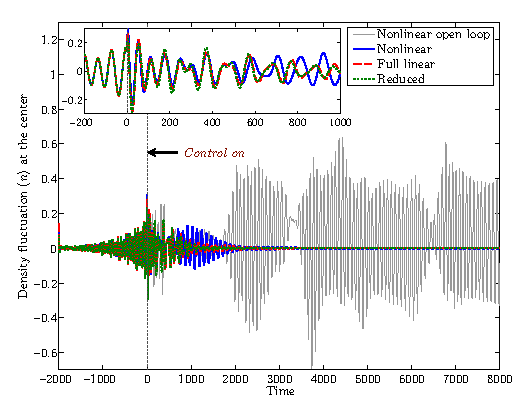
\includegraphics[width=0.9\linewidth]{observer3} 
\caption{Output feedback: 4 RHP poles / only 4 density points measured (Case \#2).}
\label{lqg4b}
\end{figure}

\begin{figure}[htbp]
\centering
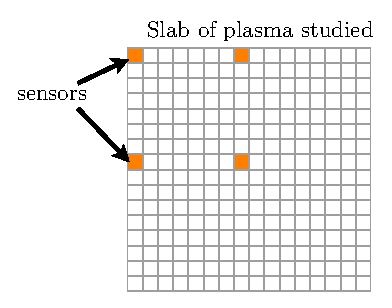
\includegraphics[width=0.5\linewidth]{observer4}
\caption{Location of the sensors.}
\label{lqg4a}
\end{figure}

The compensator stabilizes the unstable equilibrium point and furthermore the observer reconstructs the reduced order model states accurately. Initially the observer has no information about the states (the initial state estimate is $\hat x = 0$), but it quickly converges to and follows the actual states. More detailed results can be found in Chapter~\ref{chapter7}.

\begin{table}[htbp]
	\centering
	\caption{Gain margin (GM) and phase margin (PM) deduced from the loop gain of the sensitivity function}
	\label{table4c}
	\begin{tabular}{cccc} \\[-0.5em] \hline
		Case & \# of sensors & Gain margin & Phase margin \\ \hline
		  & 512&82.2&$56.6^\circ$   \\ 
		1  & 256& 41.3&$56 ^\circ $\\ 
		  &4 & 1.26& $11.8^\circ$ \\ \hline
		  &512 &19.3 &$54.3^\circ$ \\ 
		2  &256 & 13.5& $53^\circ$ \\ 
		  &4 & 1.32& $13.9^\circ$\\ \hline
	\end{tabular}
\end{table}

The gain margin (GM) and the phase margin (PM), which indicate the amount by which the actual dynamics can differ from the model (either in gain or phase) before the closed-loop system loses stability, are computed for different numbers of sensors: the full state (512 sensors), the full density field (256 sensors), and just the 4 points of the density field illustrated on Figure~\ref{lqg4a} (4 sensors). The results are shown in Table~\ref{table4c} for Cases \#1 and \#2. The cases with only 4 sensors have very small stability margins, indicating that the model needs to be very accurate in order for the controllers to stabilize the equilibrium.
However, the case where only the full density field is known would work well has the gain and phase margins are indicative of a robust controller.

\section{Conclusion}

This work introduced the technique of developing a reduced-order model of the input-output dynamics and extended it to a plasma physics problem.

In this Hasegawa-Wakatani problem, stabilizing controllers based on reduced-order linear models have been developed and applied to an unstable state and it was shown that these linear controllers applied to the full nonlinear simulations were fairly successful at suppressing the drift wave turbulence  and stabilizing the density and ion vorticity fields in the neighborhood of a chosen equilibrium point.

It was assumed for simplicity that the dimension of the unstable eigenspace is small and the corresponding global modes can be numerically computed. Building the reduced order model treats the unstable subspace exactly, and truncates from the stable subspace only.
 
Even if the actuator and sensors considered here are not practically realizable, the methodology presented can be extended to work with more realistic actuators and sensors.
Using and amplifying the zonal flow, for instance indirectly using RF waves to influence poloidal mean flow~\cite{LeBlanc1999}, would be a smart choice of actuator because of its (natural) attenuation effect: the generated zonal flow could reduce the drift wave turbulence.

Adding more actuators and improving their design will also provide better control. Here, the whole study was done with only one actuator and in some cases, the stabilization of the whole density and vorticity fields was possible.
Furthermore, the choice of sensor locations was not optimal either for the given actuator, and different choices for sensor measurements may lead to improved performance. 



\chapter{Rotation control problem}

Toroidal rotation control is the core problem of this thesis, due to its direct applicability to the new NSTX-U device.

Initially, this work focused on the previous generation of the NSTX device (before the upgrade) because experimental data was available to explore and use.
But since the device was offline at that time due to the construction for the upgrade, it was impossible to perform live experiments to test the rotation controller.
We therefore used numerical simulations generated using the TRANSP code~\cite{Budny94} (detailed later on) as a device proxy instead of real-time experiments to test the designed controller.

When we started focusing on the upgraded device NSTX-U, the device was not ready for rotation testing yet, so we chose to keep using the TRANSP upgraded models as our control objective.
For NSTX-U rotation control, beside of the toroidal rotation we added another controllable parameter; the total stored energy, that wasn't included in the NSTX work. 


We are going to present the results of modeling and control for both devices, NSTX and NSTX-U, while highlighting the main differences for each one. More details and results can be found  for NSTX in chapter~\ref{rot1&} and NSTX-U in chapter~\ref{rot2&}. 


\section{Modeling of the plasma rotation}

Rotation is essential to the performance of all present day tokamaks. Rotation can stabilize instabilities in plasma and suppress plasma turbulence, making possible the maintenance of the plasma in high temperature with less power and reduced operating costs. 

Rotation is considered here exclusively driven by external torques through the use of neutral beams injectors which heat the plasma and cause it to spin (collisionality).

Consider the transport of toroidal angular plasma momentum in a tokamak with the assumption of axisymmetry.  To facilitate the analysis, an arbitrary flux surface average $\rho \in [0,1]$ is used, where $\rho = 0$ and $1$ denote the center and the boundary of the plasma, respectively.  

Using the work of Goldston \cite{Goldston86}  and Callen  \cite{Callen09}, the angular velocity of the plasma $\omega$ can be described dynamically by the flux surface average $\left<\cdot\right>$ of the toroidal momentum equation 
\begin{multline}
  \sum_i n_i m_i \left<R^2\right> \frac{\partial \omega}{\partial t}
  + \omega \left<R^2\right> \sum_i m_i \frac{\partial n_i}{\partial t} 
  + \sum_i n_i m_i \omega \frac{\partial \left<R^2\right>}{\partial t} \\
  + \sum_i n_i m_i \left<R^2\right> \omega \left( \frac{\partial V}{\partial\rho}\right)^{-1} \frac{\partial}{\partial t} \frac{\partial V}{\partial \rho} \\
  = \left( \frac{\partial V}{\partial\rho}\right)^{-1}\frac{\partial}{\partial \rho} \left[\frac{\partial V}{\partial \rho}\sum_i n_i m_i \chi_\phi \left< R^2 (\nabla \rho)^2\right> \frac{\partial\omega}{\partial\rho}\right] \\
  - \left( \frac{\partial V}{\partial\rho}\right)^{-1}\frac{\partial}{\partial \rho} \left[\frac{\partial V}{\partial \rho}\sum_i n_i m_i \omega \left< R^2 (\nabla \rho)^2\right> \frac{v_\rho}{|\nabla\rho|}\right] \\
  - \sum_i n_i m_i \left< R^2\right> \omega \left( \frac{1}{\tau_{\phi cx}} + \frac{1}{\tau_{c\delta}}\right) + \sum_j T_j
	\label{model1}
\end{multline}
The left-hand side of the equation above represents the temporal change in the plasma toroidal angular momentum and the right-hand side terms denote respectively the one-dimensional fluid viscous term, pinch term, momentum loss due to charge exchange and field ripple, and the torque inputs (i.e., neutral beam injection and neoclassical toroidal viscosity).
\begin{itemize}
\item   $R$ is a major radial coordinate 
\item $n_i$ is the particle density 
\item $m_i$ is the particle mass for each particle species
\item $\partial V/\partial\rho$ is the differential flux surface volume
\item $\chi_\phi$ is the perpendicular (to the equilibrium magnetic field) momentum diffusivity
\item  $\tau_{\phi c x}$ is the time scale of the local momentum loss associated with charge-exchange  
\item  $\tau_{c\delta}$ is the time scale of the local momentum loss associated with field ripple
\item $T_j$ represents the various torques acting on the system
\end{itemize}

For simplicity, only the main plasma ion species (deuterium) are considered in the dynamics.
It is also assumed that the plasma cross-sectional shape is well controlled by a separate control loop and that the time variation of the mass density is small; therefore $\left< R^2 \right>$, $\left< R^2  (\nabla\rho)^2 \right>$, $ \sum_i n_i m_i $ and $\partial V/\partial \rho$ are held fixed in time.

$T_\text{NBI} $ and $T_\text{NTV}$ which represent the torques arising from neutral beam injection (NBI) and neoclassical toroidal viscosity are the two only external torques considered here.
The neutral beams are the main sources of momentum for the plasma and the NTV actuator is primarily used as a source of drag on the plasma. For NSTX, $T_\text{NBI}$ is strongest  in the plasma core, whereas $T_\text{ NTV}$ is strongest closer to the edge of the plasma. 
For NSTX-U, $T_\text{NBI}$ is spread out along the radius.

It is also assumed that the pinch term and  the momentum loss due to charge exchange are small \cite{Solomon08, Kaye09} and that the momentum loss due to  field ripple is not required, as NTV is explicitly determined in this calculation.

Although experimentally edge rotation is sometimes present, it is typically much smaller than core rotation (for NSTX, see for instance~\cite{Gerhardt14}) and important simplifications through the use of Bessel functions can be gained by assuming no edge rotation.

Incorporating all these observations into equation~(\ref{model1}), we obtain a simplified diffusion equation
\begin{equation}
 n m \left<R^2\right>
 \frac{\partial \omega}{\partial t} 
 = \left( \frac{\partial V}{\partial\rho}\right)^{-1}
   \frac{\partial}{\partial \rho} 
   \left[\frac{\partial V}{\partial \rho} n m \chi_\phi 
   \left< R^2 (\nabla \rho)^2\right> 
   \frac{\partial\omega}{\partial\rho}\right] 
   \hfill + T_\text{NBI} + T_\text{ NTV}
\label{model2}
\end{equation}
with boundary conditions
\begin{equation}
\left.\frac{\partial\omega}{\partial\rho}\right|_{\rho=0} = 0 
\quad \text{and} \quad 
\left.\omega\right|_{\rho=1} = 0
\label{model3}
\end{equation}

The resulting toroidal rotation model will be used as the rotation model for both NSTX and NSTX-U, but for NSTX-U, we will add another parameter to control which is the total stored thermal energy $W$ described by the following equation
\begin{equation}
\frac{\partial W}{\partial t}
   + \frac{W}{\tau_E}  =\sum_{i=1}^{4}{P_\textrm{\tiny{NBI}}}_i(t),
\label{energy}
\end{equation}
where ${P_\textrm{\tiny{NBI}}}_i$ represents each beam power applied, and ${\tau_E} $ represents the energy confinement time, which is modeled by an ITER 98 empirical energy confinement scaling \cite{Iter99} given by
\begin{equation}
\tau_E = H_{98y,2} 0.0562 I_{P}^{0.93} B_{T}^{0.15} n_{e}^{0.41} P_{Loss(th)}^{-0.69} R_{0}^{1.97} {\epsilon}^{0.58} \kappa^{0.78},
\end{equation}
where
\begin{itemize}
\item $I_P$ is the plasma current
\item $B_T$ is the toroidal magnetic field
\item $n_e$ is the line-averaged electron density 
\item $R_0$ is the major radius
\item $\epsilon$ is the inverse aspect ratio
\item $\kappa$ is the elongation
\item $P_{Loss(th)}$ is the loss power
\item $H_{98y,2} $ is interpolated from a user-supplied waveform
\end{itemize}

In order to control the toroidal momentum of the plasma in the tokamak, equation~(\ref{model2}) uses two actuators, the neutral beam injection (NBI) and the neoclassical toroidal viscosity (NTV). 

\begin{figure}
\centering
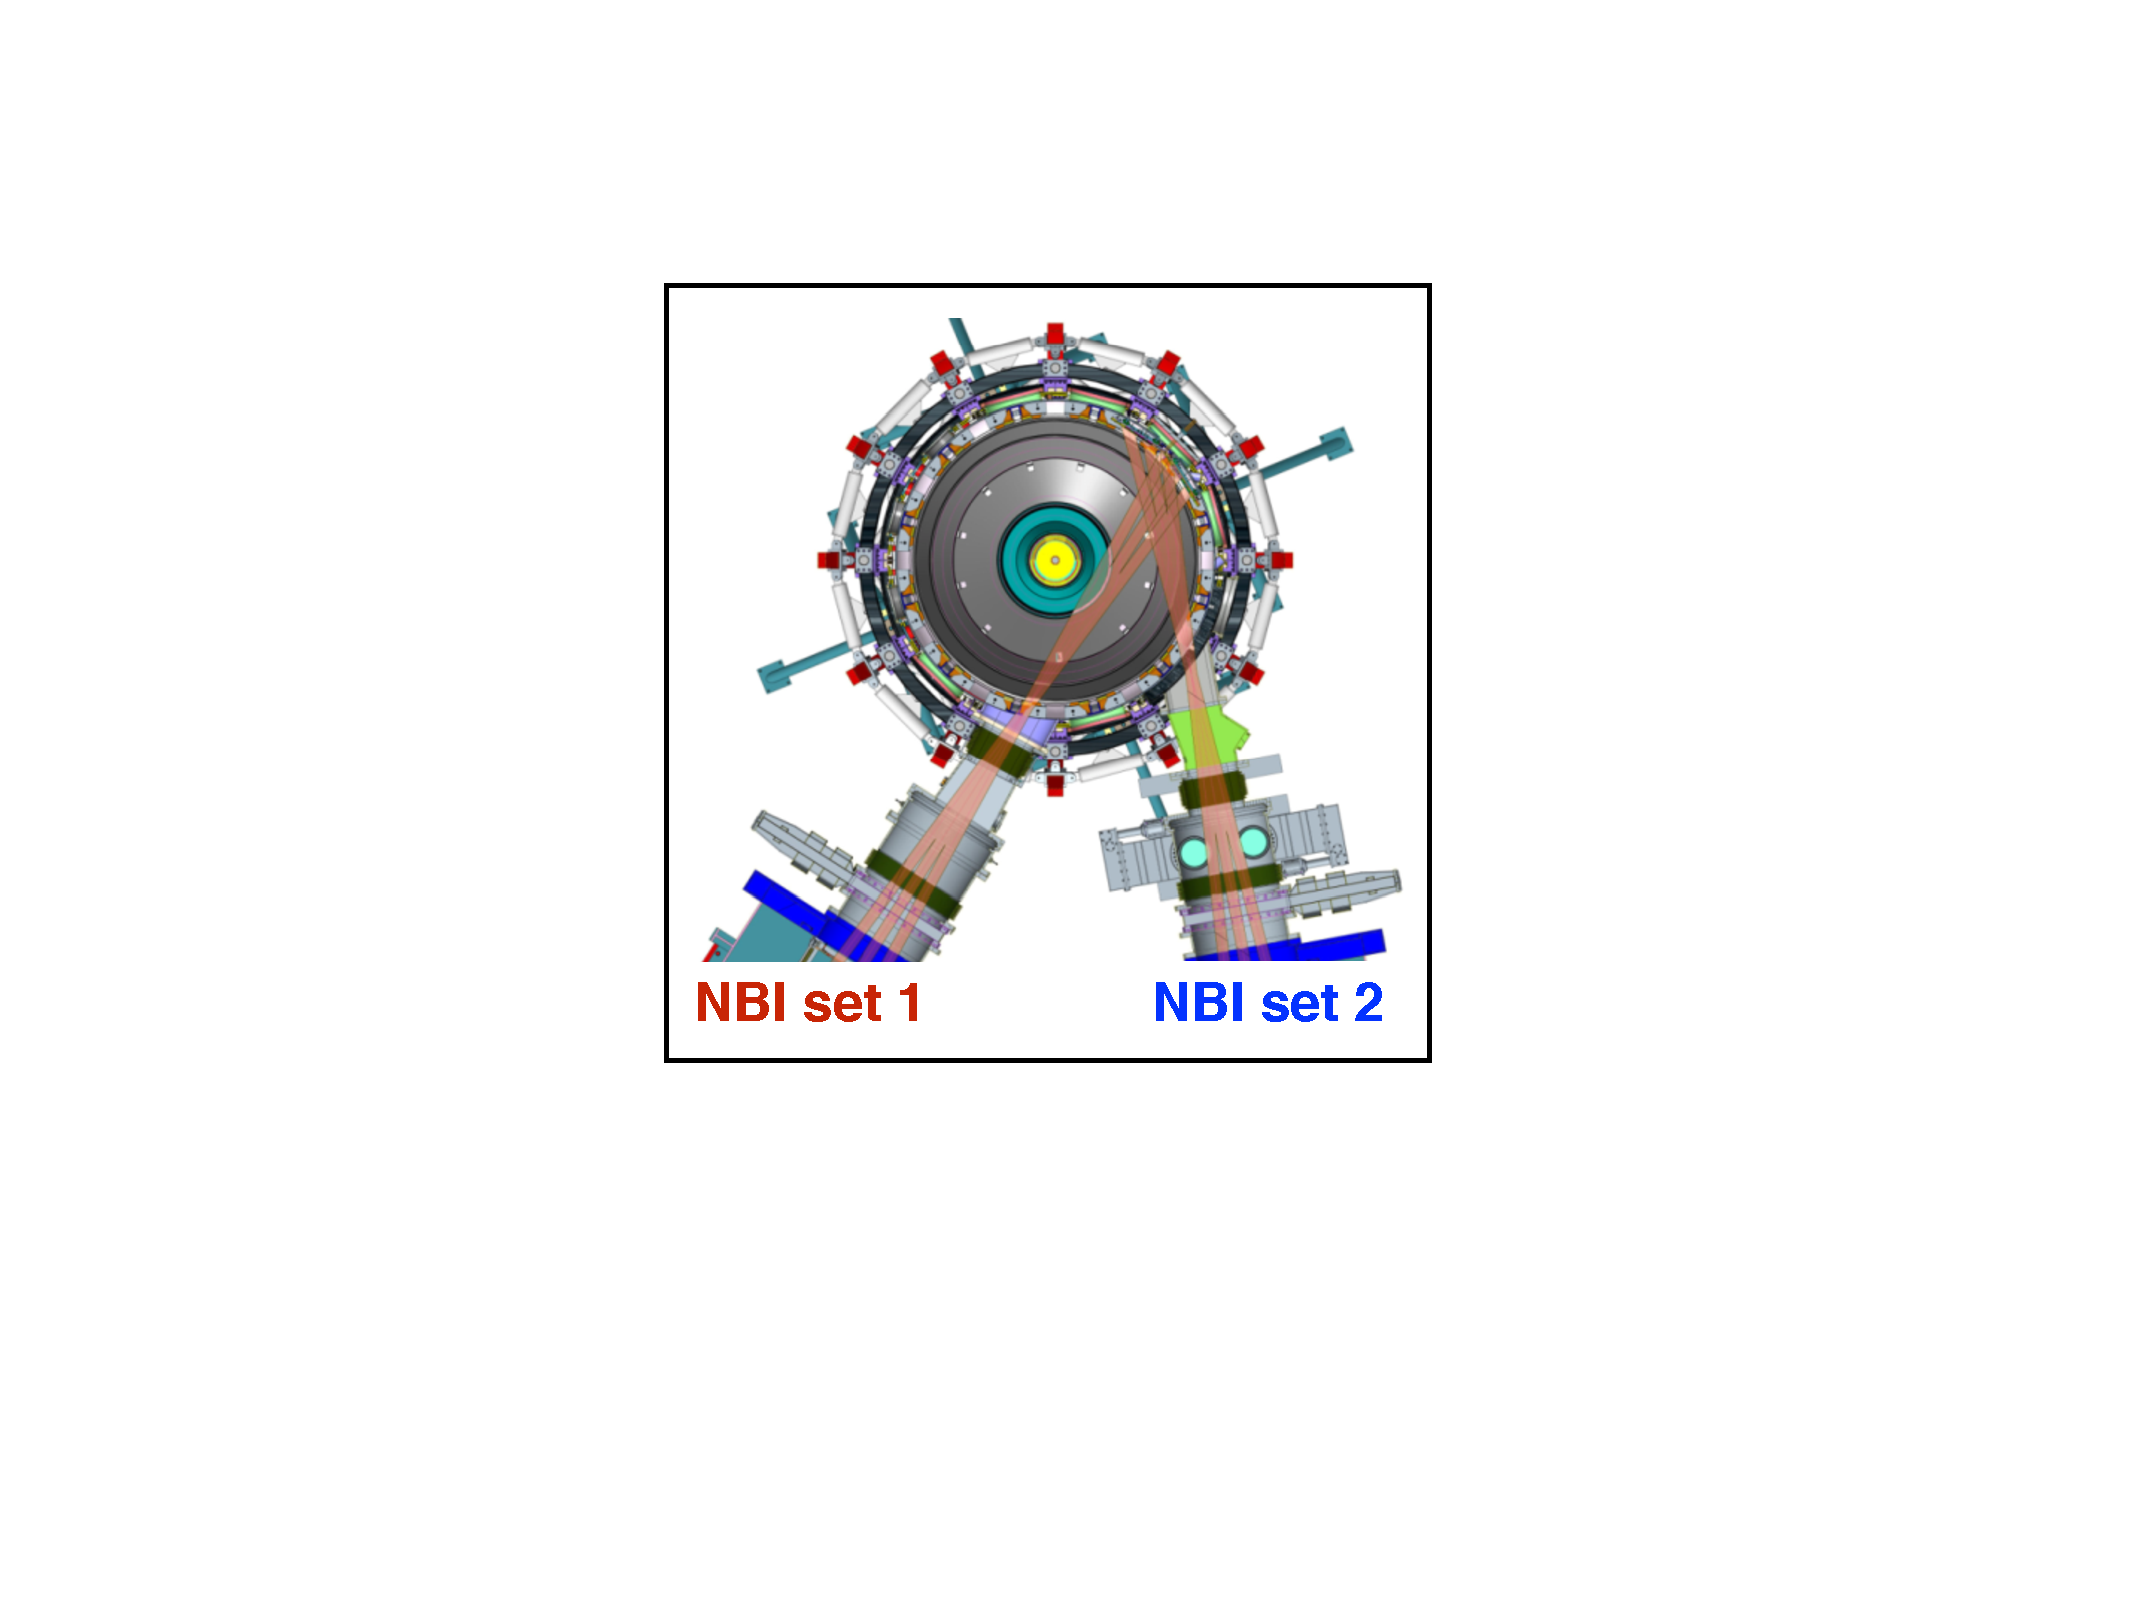
\includegraphics[width=0.6\linewidth]{nnbbii}
\caption{Illustration of the neutral beam injection (NBI) devices for NSTX-U with an inside view from the top of the tokamak. (Figure courtesy of PPPL.)}
\label{figmod6}
\end{figure}

The main difference between NSTX and NSTX-U is the increase in the number of actuators from one (actually three beam powers but modeled as a single one for simplification due to their similarities) to four actuators which consist of the addition of the three new beams separately to the original single simplified beam power. These new beams are considered individually because unlike in the old setting of NSTX, the new set of beams is oriented more tangentially. Figure~{\ref{figmod6}} shows the two sets of beams injectors inside the NSTX-U tokamak.

The modeling of the NBI torque begins as a product of the spatial average of the torque, $\overline{T}_\text{NBI}(t) \equiv \text{avg}_\rho T_\text{NBI}(t,\rho)$, and a function, $F_\text{NBI}(\rho)$, that represents the spatial profile.
We then have for $i=1,...,4$  
\begin{equation}
{T_\textrm{\tiny{NBI}}}_i(t,\rho) = {\overline{T}_\textrm{\tiny{NBI}}}_i(t) {F_\textrm{\tiny{NBI}}}_i(\rho).
\label{model5}
\end{equation}

\begin{figure} 
\centering
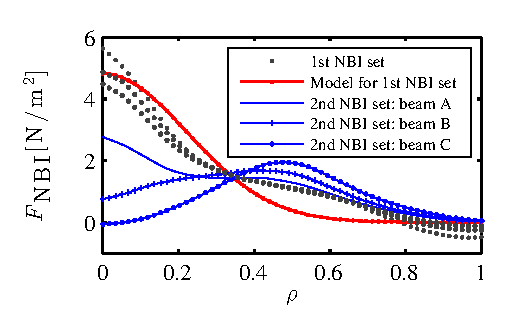
\includegraphics [width=0.7 \linewidth]{chap10/fig4} 
\caption{Spatial profile for the neutral beam torque ($F_\text{NBI} $) }
\label{figmod5}
\end{figure} 
Figure~{\ref{figmod5}} represents the footprints ${F_\textrm{\tiny{NBI}}}_i$ of the six beam power involved in the actuation. We can notice that the three beams in the first set have a similar profile (the three grey dotted lines) which is high at the core of the plasma and low towards the edge. For simplicity, it will be modeled by fitting a Gaussian function as shown by the red solid line in Figure~{\ref{figmod5}}.

The time dependency of the NBI torque $\overline{T}_\text{NBI}(t)$ is governed by the power input, $ {P_\textrm{\tiny{NBI}}}_i$ through a first-order lag
 \begin{equation}
\frac{{\partial \overline{T}_\textrm{\tiny{NBI}}}_i}{\partial t}
+ \frac{{\overline{T}_\textrm{\tiny{NBI}}}_i}{{\tau_\textrm{\tiny{NBI}}}_i}  = {\kappa_\textrm{\tiny{NBI}}}_i {P_\textrm{\tiny{NBI}}}_i(t), \label{model7}
\end{equation}
for $i=1,...,4$, where ${\tau_\text{NBI}}_i$\, are the approximate slowing down times of the fast neutral beam particles to impart energy to the bulk plasma and ${\kappa_\text{NBI}}_i$ are scalars used to normalize the neutral beam powers ${P_\text{NBI}}_i$.

Modeling the momentum loss due to the neoclassical toroidal viscosity will be based on the work done in \cite{Zhu06} from which we can design the NTV torque as the bilinear product of the coil current squared ($I^2$) with the toroidal momentum $\omega$ as follows
\begin{equation}
T_\textrm{\tiny NTV}  (t, \rho) =   K \, G(\rho) \,  \langle R^2 \rangle \:  I^2(t) \,\omega (t, \rho) .
\label{model8}
\end{equation}
where $K$ is a constant and $G$ is a Gaussian function centered towards the edge ($\mu =0.7$, $\sigma =0.1$). The control actuator input will be the squared coil current $I^2(t)$.



\section{Results on model reduction}

We present here the results obtained after applying the model reduction techniques from in Chapter~\ref{chapitre2} on a linearized version of the momentum equation \eqref{model2} that we use for modeling the toroidal rotation for both the NSTX and NSTX-U devices.

\subsection{NSTX device}
In the case of NSTX, the modeling was entirely calibrated with data obtain from a single plasma discharge ($133367$). In order to validate both the model and its reduced version, we tested this latter on different discharges.

Figure~\ref{heho_fig10} compares a simulated run of our reduced model to a different plasma discharge ($133743$) using 4 and 40 Bessel modes respectively.
Projecting the simplified model onto 40 Bessel modes yields little improvement over using only 4 modes so $N=4$ modes will be the dimension of our reduced-order model.
The relative error between the reduced model and experimental data (which is the difference between the experimental and the model rotation divided by the mean of the spatial average of the experimental rotation data) is also shown in the same figure and is less than 25\%.

\begin{figure}[htbp]
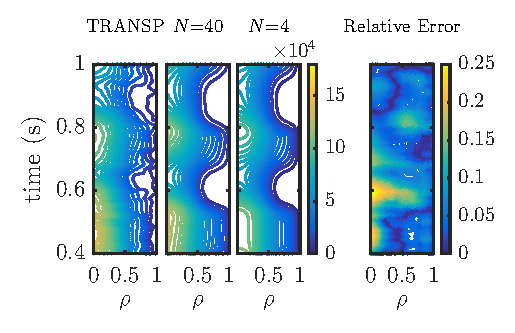
\includegraphics[width=0.9 \linewidth]{fig9}
\caption{Comparison of the rotational frequency $\omega$ for plasma discharge 133743, comparing TRANSP analysis (left), with the simplified model~\eqref{model2}, projected onto $N=40$ Bessel modes, and $N=4$ Bessel modes.  Also shown is the relative error between TRANSP and the reduced model ($N=4$).}
\label{heho_fig10}
\end{figure}


The initial condition is set to be the experimental rotational frequency at  time $t=0.4$\,s after the start up ($t=0$) and when the plasma reaches the H-mode.

An exact plasma model is not a major concern as feedback control can be designed to tolerate errors in the model. The key is to ensure the model does not deviate drastically from the actual profile in order to prevent control system instabilities from dominating plasma physics dynamics, which is the case here.

The reduced model (derived from plasma discharge 133367) is then being extensively validated against other plasma discharges in NSTX analysis.
Figure~\ref{heho1} shows how the model performs for yet another plasma discharge ($133751$). The error does not exceed 30\% for other experimental comparisons.

\begin{figure}[htbp]
\centering
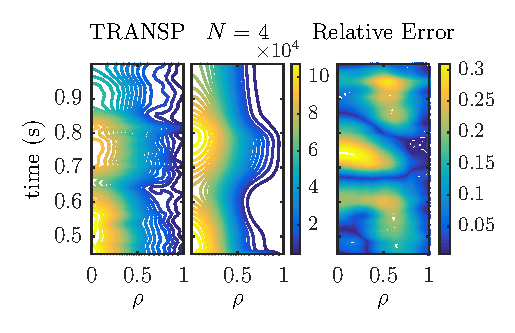
\includegraphics [width=0.8 \linewidth]{fig10}
\caption{Comparison of the rotational frequency $\omega$ for plasma discharge 133751, comparing TRANSP analysis (left), with the simplified model~\eqref{model0}, projected onto $N=4$ Bessel modes.  Also shown is the relative error between TRANSP and the reduced model ($N=4$).}
\label{heho1}
\end{figure}

The overall behavior of the plasma is captured qualitatively very well using our reduced model with fixed parameters.

\subsection{NSTX-U device}


For the case of NSTX-U, we do not have any experimental data for validation, so an exact plasma model is impossible to obtain. We rely exclusively on model based dynamical predictions. Thus TRANSP means either TRANSP analysis (data from real experiments) for NSTX or TRANSP predictive (pure simulation) for NSTX-U.

 Figure~\ref{heho2} compares a simulated run of the model versus TRANSP (prediction of plasma scenario 142301) when the first set of beams is activated combined with a chosen NTV torque.
We note that $N = 8$ Bessel modes capture the main features of the dynamics for relative errors of about 25\%.
The overall behavior of the plasma is still captured qualitatively very well, but because of many modeling uncertainties due to the lack of real time measurements, the feedback controller will be designed to tolerate errors in the model and its robustness in terms of stability and performance will be carefully studied by modeling the uncertainties of the model based on known ranges of acceptable variation of some model parameters.

We will ensure that the designed controller reaches its objectives despite these uncertainties.
\begin{figure}[htbp]
\centering
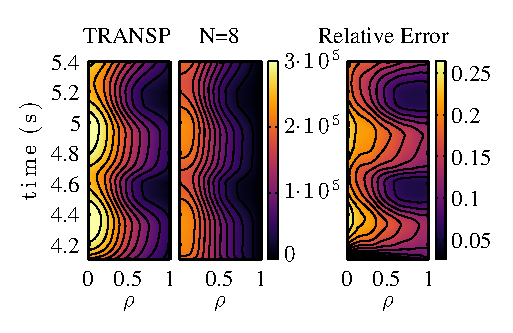
\includegraphics [width=0.8 \linewidth]{chap10/fig10} 
\caption{Comparison of the rotational frequency $\omega$ for plasma simulation, comparing TRANSP prediction (left), with the simplified model projected onto $N=8$ Bessel modes.  Also shown is the relative error between TRANSP and the reduced model ($N=8$).}
\label{heho2}
\end{figure}

\section{TRANSP implementation}

Since the NSTX device was unavailable during the upgrade construction and since experimental data is not yet available for NSTX-U, modeling and testing were done from simulated data generated using predictive TRANSP simulations.

TRANSP, a time dependent code developed at Princeton Plasma Physics Laboratory for both prediction and analysis of tokamak experimental data \cite{TRANSP16, Budny94}, is one of the primary codes used in the fusion community. Several widely used modules, including NUBEAM \cite{Pankin04} for calculating neutral beam heating and current drive are available for use within TRANSP and make it well suited for the predictive simulations required in this work where the primary actuator of our controller is variation of various beam powers.

Although the use of reduced models makes the control design process simpler, the highly coupled nonlinear nature of the tokamak can potentially lead to unexpected behavior and instabilities when controllers tuned and tested only on reduced models are experimentally tested. Therefore the intermediate step of conducting closed loop simulations of real-time control laws in the integrated modeling code framework of TRANSP before testing on real device is very important.
These predictive capabilities of TRANSP mentioned above combined with a new module that enables the stored energy to be predicted based on confinement scaling expressions (for \mbox{NSTX-U}) are going to be used to mimic the device as our original system to control. 

TRANSP has the flexibility to simulate a variety of control designs, and will enable fine-tuning of control laws, studies of robustness to scenario changes, studies of the impact of control laws on parameters not considered in the reduced models used for initial designs, and the demonstration of novel control schemes before devoting experimental time to their implementation.

The inputs to TRANSP for the rotation control are the time histories of the plasma boundary shape, total plasma current, electron temperature and density profiles, and the power, voltage, and geometry of the neutral beam injection. With these inputs, the TRANSP code (NUBEAM) is used to compute the correct neutral beam heating.

The free-boundary equilibrium is calculated using the ISOLVER equilibrium code within TRANSP \cite{Huang06}. ISOLVER computes a free-boundary solution to the Grad-Shafranov equation that has boundary and X-point locations that best match a provided target plasma boundary. The target equilibria were generated using the stand-alone version of ISOLVER, based on the NSTX-U coil set. In an iterative procedure, a free-boundary equilibrium solution is obtained, the current and pressure profiles are computed on the new equilibrium, and the equilibrium is recalculated.

In addition to equilibrium calculations, scenario studies require simulation of the ion and electron densities and thermal transport. Experiments indicate that ion heat transport is reasonably well described by neoclassical theory \cite{Kaye07, Kaye007,Valovic11}, the Chang-Hinton model \cite{Chang82} is then used to model the dynamics of the ion temperature. However, because models for electron heat transport, external fueling, impurity sources, and particle transport are not as well validated, the evolutions of electron temperature and particle densities were not modeled by first principles calculations.

To handle the remaining unmodeled quantities, some assumptions were made. First, the electron density profile was taken from an experimental profile measured on NSTX, scaled to achieve a particular Greenwald fraction \cite{Greenwald88}. The ion density was calculated by assuming a flat $Z_\text{eff} = 2$ profile with carbon as the only impurity. The electron temperature was again taken from an experimental profile and scaled to achieve a particular global confinement level. The toroidal rotation profile was also taken from experiment and scaled inversely with the density.

The modifications necessary for closed loop simulations have been implemented through the so-called Expert routine. This routine is a hook, called at various places throughout the TRANSP source code, which can be used to insert run-specific custom code into the production version of TRANSP.
A module, which contains a simplified reduced model, is provided for performing control calculations based on user-supplied data (controller matrices, desired target to reach, etc.). These calculations, along with the acquisition of \emph{real-time} measurements (simulated) and manipulation of TRANSP internal variables representing the control systems actuators (like beam power and coil current), are implemented through the Expert routine.

TRANSP typically obtains the electron temperature from an input file, a call to the Expert routine is made just after each time TRANSP accesses the temperature input data. At each of these calls, the Expert file code interpolates the thermal stored energy $W_\text{th}$ for the appropriate time based on $W_{\text{th}_a}$ and $W_{\text{th}_b}$, the predicted values at $t_a$ and $t_b$ and calculates the required scale factor for the reference profile.

In these calculations, the $n_i$, $n_e$, and $T_i$ profiles are taken from the TRANSP internal variables at the current time step. $T_i$ is calculated using the Chang-Hinton model, and $n_i$ is calculated by assuming a $Z_\text{eff}$ profile and carbon as the only impurity.

\section{Results on control}

In this section, results of the application of the reduced order model based compensator detailed in Chapter~\ref{rot1&} on the momentum equation (Reduced and TRANSP models) are shown for both the NSTX and NSTX-U devices.

Because the controllers will be applied on real time experiments, they have to be discretized. The discretization is not explicitly expanded in the background chapter~\ref{chapitre2} but can be found in details in any control reference book \cite{AandM, SandP}.

For our particular problem, converting to a discrete model was a subtile intermediate step that was applied after defining the linear simplified model and before applying the model reduction using the Matlab command ($c2d$). Therefore the design of the controller was also done in discrete time.

There are important constraints on the two type of actuators that have to be considered. Some of these constraints are made for the safety of the operations, some of them reflect the practicability and the feasibility of some requests to the device. The constraints will be inserted into the dynamics equations so that the controller will have to consider them during the closed loop.

The coil current is constrained between two numerical values, 0 and 3,000 amperes, and because its response is fast compared to the dynamics of the system, it can be assumed to be applied instantaneously (no time delay to consider for this actuator.)

Even if we have so far been treating the the first set of NBI actuators as a single source outputting between 2 and 6\,MW of power for both NSTX and NSTX-U, it is actually composed of 3 beams. Each beam can either be on and produce 2\,MW of power or off and produce 0\,MW. The three other beams will be considered separately but still have to follow beam power constraint which is that each beam can only be switched on or off a maximum of 20 times per plasma discharge to prevent device fatigue issues, and that there is a refractory period of 10\,ms after each switch during which the beam cannot be switched again.

Due to diagnostic considerations, one of the first set of NBI sources is typically always on, and so the overall injected power is considered to be between $2$ and $6$ MW for NSTX and  between $2$ and $12$ MW for NSTX-U.

These physical restrictions are the other reason that constrains the model and the controller to be discrete and to use Pulse Width Modulation (PWM) for the beam power actuation in order to obtain control requested values between 2 and 6\,MW for NSTX (resp. 2 and 12\,MW for NSTX-U).


\begin{figure}
	\centering
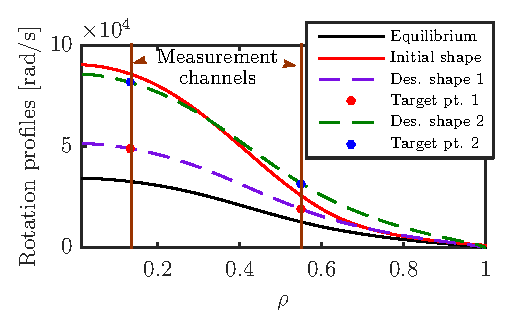
\includegraphics[width=0.7 \linewidth]{fig100}
\caption{Rotation profiles: definition of the initial profile, equilibrium profile $w_0$ used for the linearization and the desired profiles to reach $w_d$. The measurement points $r$ are the intersections of the different profiles with the measurement channels}
\label{go1}
\end{figure}

At the beginning of each duty cycle, the controller sets the requested power. During the duty cycle, the beams switch on and off at most once to minimize the number of switches. Because of this and the 10\,ms refractory period, the exact requested power cannot always be met.
The longer the duty cycle, the better for the device because it means less commands switches so less fatigue, but a longer duration introduces a longer controller lag which impairs performance.

\subsection{NSTX device}

In the case of NSTX, Figure~\ref{res1} and Figure~\ref{res2} compares the rotation measurements when the PWM controller is applied to both the reduced-order model and the TRANSP predictive model in order to reach two targets, one at $t = 0.5$s, and the other starting at $t=0.7$s.
Before $t=0.5$\,s, both models are not controlled (open loop), at $t = 0.5$\,s, the controller is turned on (closed loop), and the goal is to reach the first target profile measurement points defined by the two red dots in Figure~\ref{go1}. At $t = 0.7$\,s, the  target profile changes to the second one which is defined by the two blue dots in Figure~\ref{go1}.

The green line represents the reduced-order model outputs, the blue line represents the TRANSP model. The oscillations are due to the modulations that occurs on each of the beam power source. The total beam power is represented in Figure~\ref{res2}(b). The coil current in this case (Figure~\ref{res2}(a)) changes to compensate for when the beam power is too high in order to decrease the toroidal rotation and thus limit the rotation overshoot.
In this case, the duty cycle duration (6\,ms) is smaller that the the 10\,ms refractory period.
The resulting rotation measurements are oscillatory but the amplitude is damped. The trade off is that we have to activate the controller more often and thus formulate more requests to the real device.
The reduced-order model is very close to the TRANSP model which again shows that the simplified model gives us a good qualitative approximation of the TRANSP rotation prediction model.

\begin{figure}[htbp]
	\centering
	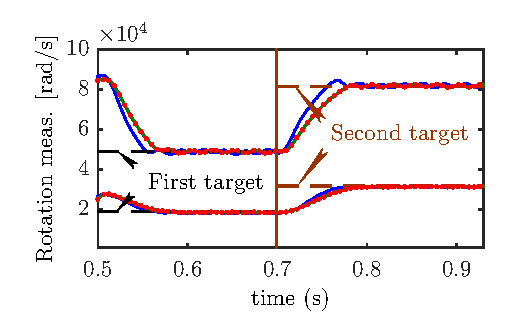
\includegraphics[width= 0.7\linewidth]{fig18}
	\caption{Comparison of the rotation measurements when PWM applied for both the reduced-order model (green lines) and the TRANSP predictive model (blue lines). The red dots represents the cycle times (every $0.006 s$).}
	\label{res1}
\end{figure}

\begin{figure}[htbp]
	\centering
	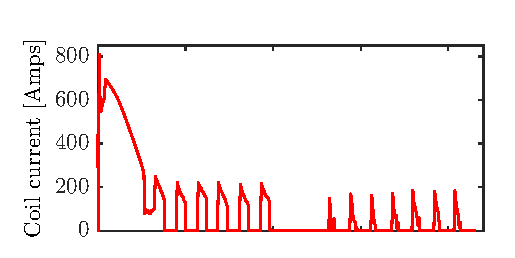
\includegraphics[width=0.7 \linewidth]{fig19a} \adjustbox{raise=11.3em,lap=-3.2em}{(a)} \\[-0.5em]
	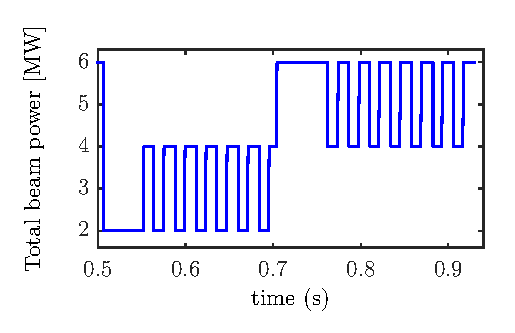
\includegraphics[width=0.7 \linewidth]{fig19b} \adjustbox{raise=6.2em,lap=-3.2em}{(b)}
	\caption{Time evolution of the coil current and the overall beam power (cycle time $0.006 s$). }
	\label{res2}
\end{figure}

Note that although the coil current is not directly pulsed, indirect pulses induced by the beam powers can be seen on Figure~\ref{res2}(a).
Similar pulses have been observed to sometimes trigger ELMs~\cite{Canik10} which can be very disruptive for control.
A low pass filter could be used to tame these coil current pulses at the cost of slightly diminishing control performance.

%\subsection{Study of robustness in stability and performance}
%
%It is very important to assess not only that the closed-loop system is stable and has good performance, but that stability and performance are conserved in the face of uncertainty.
%This was particularly critical when we designed a controller for NSTX-U as there was no experimental data available at that time, only models and parameters extrapolated from NSTX.
%
%We started by checking that our nominal system was stable and by defining performance specifications.
%Performance is a trade-off between getting a fast response while tracking the reference signal $y_d$ and making sure that measurement noise and other disturbances are not amplified too much by the feedback loop.
%We consider the three sources of disturbances shown on Figure~\ref{fig:example_disturbances}: an input disturbance $d_u$ affecting the input of $G$, an output disturbance $d_y$ affecting the output of $G$, and sensor noise $n$ which does not directly affect the output of $G$ but enters the controller nevertheless.
%
%\begin{figure}[htbp]
%	\centering
%	\begin{tikzpicture}
%		\node (yd) {$y_d$};
%		\node[block, right=0.5 of yd] (F) {$F$};
%		\node[sum, right=0.6 of F] (sum u) {};
%		\node[above=0.4 of sum u] (du) {$d_u$};
%		\node[block, right=of sum u] (G) {$G$};
%		\node[sum, right=0.7 of G] (sum y) {};
%		\node[above=0.4 of sum y] (dy) {$d_y$};
%		\node[junction, right=0.4 of sum y] (out) {};
%		\node[right=0.5 of out] (y) {$y$};
%		\node[block, below=0.4 of G] (K) {$K$};
%		\node[sum] (sum n) at (K-|out) {};
%		\node[right=0.5 of sum n] (n) {$n$};
%		
%		\draw[connector] (yd) to (F);
%		\draw[connector] (F) to (sum u);
%		\draw[connector] (du) to (sum u);
%		\draw[connector] (sum u) to node[above] {$u$} (G);
%		\draw[connector] (G) to (sum y);
%		\draw[connector] (dy) to (sum y);
%		\draw[connector] (sum y) to (out) to (y);
%		\draw[connector] (out) to (sum n);
%		\draw[connector] (n) to (sum n);
%		\draw[connector] (sum n) to (K);
%		\draw[connector] (K) -| node[right, pos=0.98] {$\scriptstyle -$} (sum u);
%	\end{tikzpicture}
%	\caption{Input disturbance $d_u$, output disturbance $d_y$, and sensor noise $n$.}
%	\label{fig:example_disturbances}
%\end{figure}
%
%We define nominal performance by choosing upper bounds on the transfer functions from these disturbance inputs to either the output $y$ (or equivalently, to the error $e = y - y_d$) or to the input $u$.
%There are two important aspects to consider when choosing specifications for these transfer functions.
%The \emph{static} aspect is given by the \emph{peaks} (maximum values) which are related to the quality of the response.
%The \emph{dynamic} aspect is given by the \emph{bandwidth frequency} which is related to the speed of the response.
%In general, a large bandwidth means better performance since high frequency signals are more easily passed on to the outputs, so the rise time is improved, but it also indicates a system which is sensitive to noise and model uncertainties.
%
%The five distinct transfer functions of interest are shown in the matrix below:
%\begin{equation}
%	\renewcommand\arraystretch{0.8}
%	\begin{bmatrix} y \\ u \end{bmatrix} =
%	\begin{pmatrix} S_o G & S_o & -To \\ S_i & S_i K & S_i K \end{pmatrix}
%	\begin{bmatrix} d_u \\ d_y \\ n \end{bmatrix}
%\end{equation}
%where $S_o = (I + G K)^{-1}$ is the output sensitivity, $T_o = (I + G K)^{-1} G K = S_o G K$ is the output complementary sensitivity, and $S_i = (I + K G)^{-1}$ is the input sensitivity.
%
%The sensitivity (both input and output) is of particular importance since it is a factor in most of these transfer functions (note that $S_o G = G S_i$ and $S_i K = K S_o$).
%For both $S_o$ and $S_i$, we choose the upper bound such as to guarantee a bandwidth of 25\,Hz and a maximum peak of 1.9 (which guarantees a stability margin of 0.53).
%In the control literature, a maximum peak sensitivity of 2 or less is considered good for most intents and purposes.
%We also want the output complimentary sensitivity to start rolling off at 200\,Hz maximum, have a maximum 20\% amplification at low frequencies.
%We want $S_o G$ to roll-off at no more than 50\,Hz and have at least a 14\,dB attenuation.
%To limit actuator use, we want $S_i K$ to have a bandwidth of at least 10\,Hz and no more than 40\,dB amplification.
%All the bounds can be seen on Figure~\ref{fig:example_robust_performance}.
%
%Next we want to introduce perturbations in our system.
%Without data from NSTX-U, we choose to introduce parameter uncertainty.
%The two parameters that are most likely to be varying significantly from their nominal value are $\chi_\phi$ and $\tau_E$.
%Let $\bar{\chi}_\phi$ be the nominal value (which depends on the radial variable $\rho$) of $\chi_\phi$, and
%let $\bar{\tau}_E$ be the nominal value of $\tau_E$.
%We assume that the perturbed model $G_p$ is built from perturbed values of the parameters ${\chi_\phi}_p$ and ${\tau_E}_p$, where
%${\chi_\phi}_p$ is a random perturbation of bounded magnitude around $\bar{\chi}_\phi$ generated using 1D Perlin noise, with bounds $0.9 \bar{\chi}_\phi$ and $1.1 \bar{\chi}_\phi$, and ${\tau_E}_p = \mu \cdot \bar{\tau}_E$ with $\mu \in [0.9,1.1]$.
%
%By superimposing the Nyquist plots of many perturbed plants, we observe that right multiplicative uncertainty adequately represents the pattern we obtain.
%Thus we define a perturbed plant as
%\begin{equation} \label{eq:multiplicative}
%	G_p = G (I + W_1 \Delta W_2),
%\end{equation}
%where $W_1$ and $W_2$ are weighting transfer function matrices, and $\Delta$ satisfies $\|\Delta\|_\infty < 1$.
%For simplicity, $W_1$ is taken to be the identity matrix.
%A block diagram of the perturbed plant is shown in Figure~\ref{fig:example_multiplicative_foo}.
%
%\begin{figure}[htbp]
%	\centering
%	\begin{tikzpicture}
%		\node (u) {$u$};
%		\node[junction, right=0.5 of u] (in) {};
%		\node[coordinate, right=1 of in] (below W2) {};
%		\node[block, above=0.5 of below W2] (W2) {$W_2$};
%		\node[coordinate, right=1.7 of below W2] (below Delta) {};
%		\node[block, above=0.5 of below Delta] (Delta) {$\Delta$};
%		\node[coordinate, right=1.7 of below Delta] (below W1) {};
%		\node[block, above=0.5 of below W1] (W1) {$W_1$};
%		\node[sum, right=0.9 of below W1] (sum) {};
%		\node[block, right=0.5 of sum] (G) {$G$};
%		\node[right=0.5 of G] (y) {$y$};
%		
%		\draw[connector] (u) to (in) to (sum);
%		\draw[connector] (sum) to (G);
%		\draw[connector] (in) |- (W2);
%		\draw[connector] (W2) to (Delta);
%		\draw[connector] (Delta) to (W1);
%		\draw[connector] (W1) -| (sum);
%		\draw[connector] (G) to (y);
%	\end{tikzpicture}
%	\caption{Perturbed model $G_p = G (I + W_1 \Delta W_2)$}
%	\label{fig:example_multiplicative_foo}
%\end{figure}
%
%Then we superimpose the Bode plots of $G^{-1}{G_p} - I$ for many perturbed plants to find a suitable weight $W_2$.
%
%\begin{figure}
%	\centering
%	\begin{tikzpicture}
%		\node[font=\large\bfseries] at (-0.25,1.25) {a)};
%		\path (0,1.25) -- ++(down:2.75);
%
%		\node[sum] (sum) {};
%		\node[junction, right=0.5 of sum] (in) {};
%		\node[coordinate, right=of in] (below W2) {};
%		\node[block, above=0.4 of below W2] (W2) {$W_2$};
%		\node[coordinate, right=2 of below W2] (below Delta) {};
%		\node[block, above=0.4 of below Delta] (Delta) {$\Delta$};
%		\node[coordinate, right=2 of below Delta] (below W1) {};
%		\node[block, above=0.4 of below W1] (W1) {$W_1$};
%		\node[sum, right=of below W1] (out) {};
%		\node[block, right=0.5 of out] (G) {$G$};
%		\node[coordinate, right=0.5 of G] (end) {};
%		\node[coordinate] (above K) at ($(sum)!0.5!(end)$) {};
%		\node[block, below=0.6 of above K] (K) {$K$};
%		
%		\draw[connector] (sum) to (in) to (below W2) to (below Delta) to (below W1) to (out) to (G);
%		\draw[connector] (G) to (end) |- (K);
%		\draw[connector] (K) -| node[right, pos=0.98] {$\scriptstyle -$} (sum);
%		
%		\draw[connector] (in) |- (W2);
%		\draw[connector] (W2) to node[above] {$u_\Delta$} (Delta);
%		\draw[connector] (Delta) to node[above] {$y_\Delta$} (W1);
%		\draw[connector] (W1) -| (out);
%	\end{tikzpicture}
%	\begin{tikzpicture}
%		\node[font=\large\bfseries] at (-2,0.5) {b)};
%		\path (0,0.5) -- ++(down:2.75);
%		
%		\node[block] (Delta) {$\Delta$};
%		\node[block, below=0.5 of Delta] (M) {$M$};
%		
%		\node[coord, right=0.6 of M] (right) {};
%		\node[coord, left=0.6 of M] (left) {};
%		
%		\draw[connector] (M.east) to (right |- M) to node[right] {$y_\Delta$} (right |- Delta) to (Delta);
%		\draw[connector] (Delta) to (left |- Delta) to node[left] {$u_\Delta$} (left |- M) to (M);
%	\end{tikzpicture}
%
%	\caption{Block diagrams of the loop of the perturbed closed-loop system stripped of all exogenous inputs and outputs. \textbf{a)} Expanded system. \textbf{d)} $M \Delta$ structure for robust stability analysis.}
%	\label{fig:example_diagram_perturb_foo}
%\end{figure}
%
%To assess robust stability, we rearrange our system of Figure~\ref{fig:example_diagram_perturb_foo}a into the $M \Delta$ configuration of Figure~\ref{fig:example_diagram_perturb_foo}b to obtain the transfer function block matrix $M$:
%\begin{equation}
%	M = -W_2 K S_o G W1.
%\end{equation}
%
%Since our nominal closed-loop system is stable and since the largest singular value of $M$ is less than 1 for all frequencies (Figure~\ref{fig:example_robust_stability}), by theorem 8.4 of~\cite{SandP}, our closed-loop system is robustly stable.
%
%\begin{figure}[htbp]
%	\centering
%	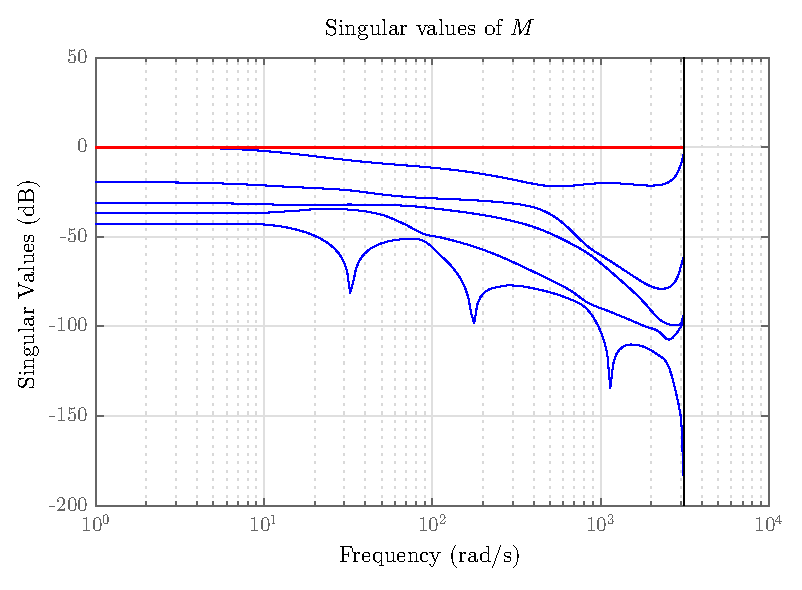
\includegraphics{chap10/robust_stability}
%	\caption{Robust stability. The singular values of $M$ are always less than 1.}
%	\label{fig:example_robust_stability}
%\end{figure}
%
%
%To test for robust performance, we generate many perturbed plants and check that each one of them satisfies the performance specifications by superimposing the Bode plots of the singular values of the perturbed plants (Figure~\ref{fig:example_robust_performance}).
%We verify that our controller has robust performance for the set of perturbed plants and the specifications stated above.
%
%\begin{figure}[htbp]
%	%\centering
%%	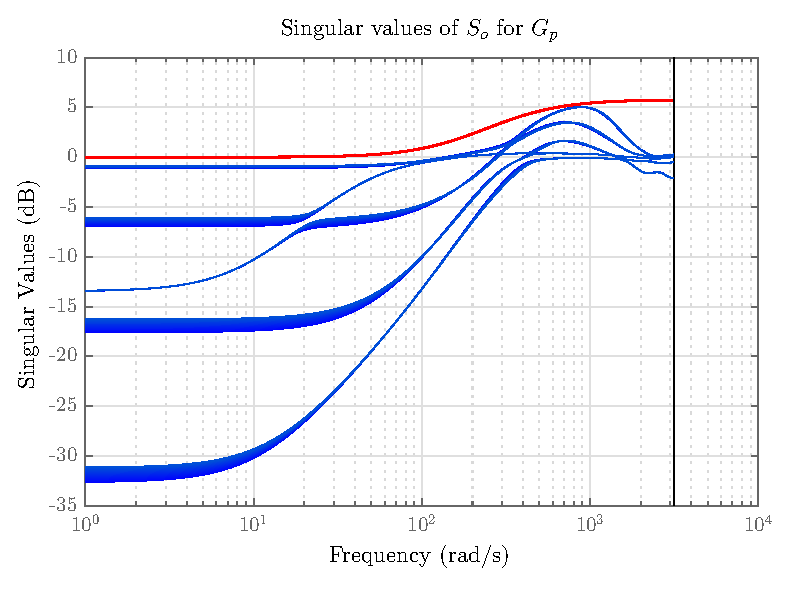
\includegraphics[width=0.5\linewidth]{chap10/robust_performance_So}%
%%	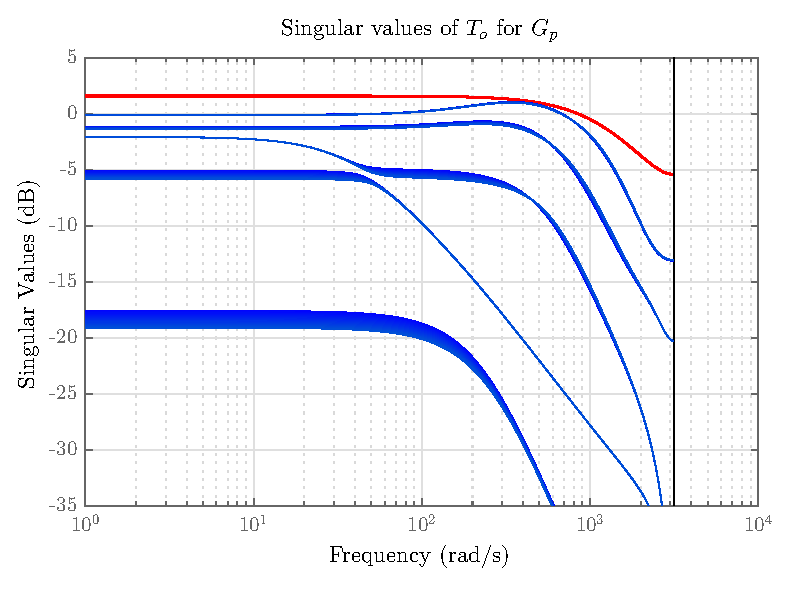
\includegraphics[width=0.5\linewidth]{chap10/robust_performance_To}
%%	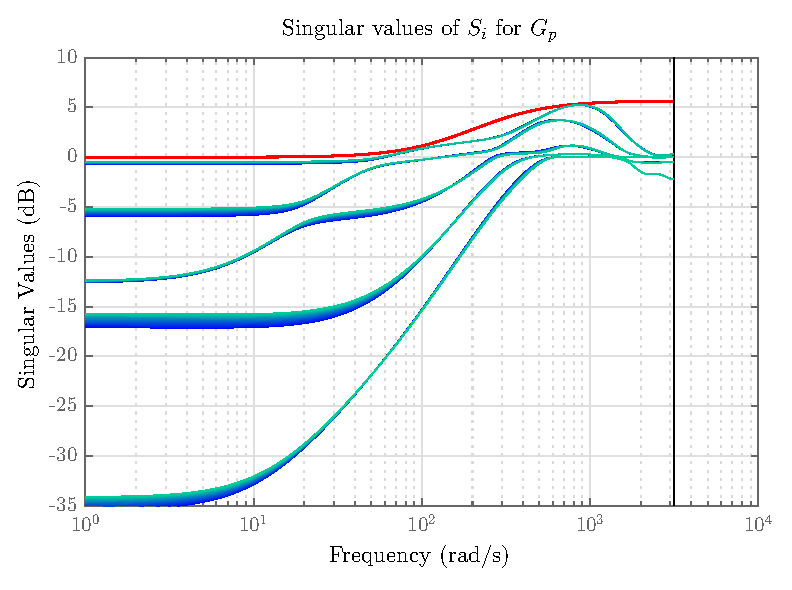
\includegraphics[width=0.5\linewidth]{chap10/robust_performance_Si}%
%%	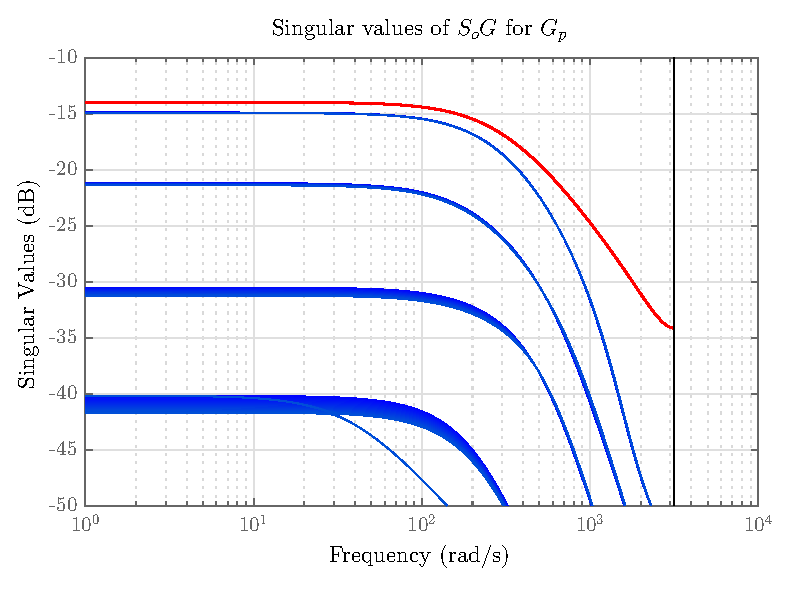
\includegraphics[width=0.5\linewidth]{chap10/robust_performance_SoG}
%%	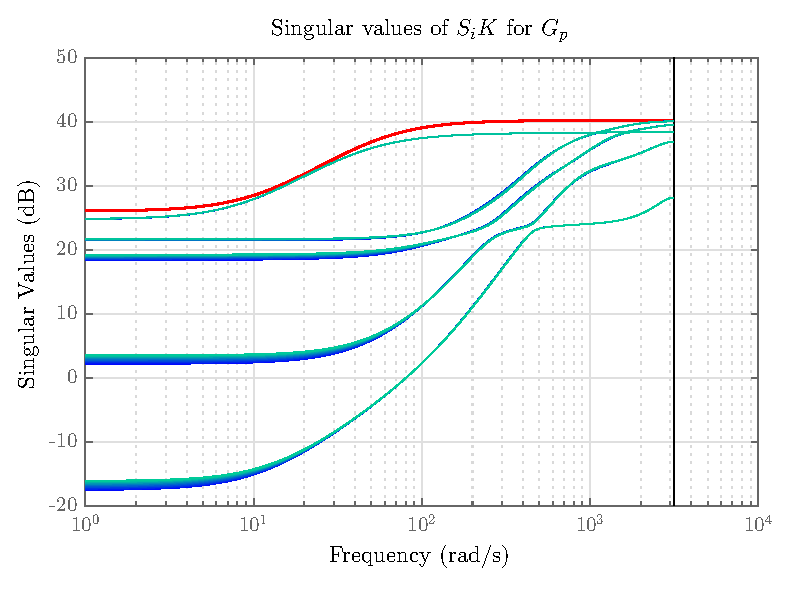
\includegraphics[width=0.5\linewidth]{chap10/robust_performance_SiK}
%	\caption{Robust performance.
%		The singular values of the transfer functions of 256 perturbed plants are shown superimposed in blue.
%		All perturbed transfer functions meet the performance specifications indicated by their upper bound in red.}
%	\label{fig:example_robust_performance}
%\end{figure}

\subsection{NSTX-U device}

The principal differences between the NSTX and NSTX-U control problems are the addition of the stored energy as a controllable parameter and the addition of the second NBI set which brings the number of control inputs from 2 to 5. To facilitate the design of the controller, since it is more convenient to work with a system that has as many inputs as outputs, we added two additional rotation profile measurement points which brings the number of control outputs (sensors) to 5 as well.

The addition of the stored energy introduces a challenge that was not present during the NSTX controller design.
Since the stored energy is linked to the beam powers by equation~\eqref{energy}, one degree of freedom in selecting the beam powers (which affect both the rotation and the stored energy) is lost, so it becomes harder to reach both the target rotation profile and the target stored energy simultaneously.
To counteract this restriction, we decided to add an integrator inside the controller which uses accumulated tracking errors to adjust the control commands. However combining an integrator with saturated inputs yields the well-known \emph{integrator windup} problem which tend to increase overshoot of the targets, so we also used a standard back calculation anti-windup method which is described in~\cite{AandM}. However, while the addition of the integrator gives us more flexibility for the controller design, actuator saturation combined with the effects of equation~\eqref{energy} imposes a trade-off that prevents us from tracking both the rotation and the stored energy perfectly depending on the choice of targets.
Assigning high costs to the tracking error can drastically improve the performance of the controller when actuators do not have any constraints, but it can create destabilizing oscillations when actuators saturate.

The other important difference between the NSTX and NSTX-U while designing a controller is that due to the lack of experimental data, the models for NSTX-U are much more uncertain. Therefore we proceed to analyze the robustness in terms of stability and performances of the NSTX-U controller to model uncertainty caused by variation of some parameters of the model from their nominal values.

Once we are satisfied with this design of controller, the following step is testing it on TRANSP predictive simulation.

\begin{figure}[htbp]
	\centering
	\begin{overpic}[width=0.8 \linewidth]{chap10/rotnstxu}
		\put(18,51){$\leftarrow$ Control on}
		\put(24.2,47){1st target}
		\put(55,51){Control on $\rightarrow$}
		\put(55,47){2nd target}
	\end{overpic}
	\caption{Comparison of the rotation measurements when PWM is applied for both the reduced-order model (red lines) and the TRANSP predictive model (blue lines).}
	\label{rotnstxu2}
\end{figure}

\begin{figure}[htbp]
	\centering
	\begin{overpic}[width=0.8 \linewidth]{chap10/energynstxu}
		\put(27,26){\tikz{
			\coordinate (O);
			\node (label) at (1,-1) {1st target};
			\draw[->,thick] (label) to (O);
		}}
		\put(77,41){\tikz{
			\coordinate (O);
			\node (label) at (1,1) {2nd target};
			\draw[->,thick] (label) to (O);
		}}
	\end{overpic}
	\caption{Stored energy measurements when PWM is applied for the TRANSP predictive model (blue line).}
	\label{energynstxu2}
\end{figure}


\begin{figure}[htbp]
	\centering
	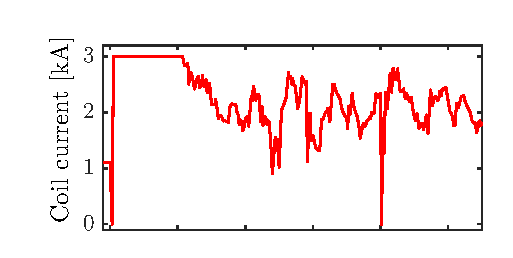
\includegraphics[width=0.8 \linewidth]{chap10/currentnstxu} \adjustbox{raise=11em,lap=-0.8em}{(a)} \\[-0.5em]
	\begin{overpic}[width=0.8 \linewidth]{chap10/NBInstxu}
		\put(77,31){\tikz{
			\draw[thick,fill=white] (0,0.1) rectangle (3,2.4);
			\draw[ultra thick, blue] (0.1,2) -- (0.4,2);
			\node[anchor=west] at (0.4,2) {Beam set 1};
			\draw[ultra thick, red] (0.1,1.5) -- (0.4,1.5);
			\node[anchor=west] at (0.4,1.5) {Beam set 2A};
			\draw[ultra thick, black] (0.1,1) -- (0.4,1);
			\node[anchor=west] at (0.4,1) {Beam set 2B};
			\draw[ultra thick, green!50!black] (0.1,0.5) -- (0.4,0.5);
			\node[anchor=west] at (0.4,0.5) {Beam set 2C};
		}}
	\end{overpic} \adjustbox{raise=15.5em,lap=-0.8em}{(b)}
	\caption{Time evolution of the coil current and the beam power}
	\label{inputnstxu2}
\end{figure}

Figure~\ref{rotnstxu2} compares the rotation measurements when the PWM controller is applied to both the reduced-order model and the TRANSP predictive model in order to reach two targets, one at $t = 4.2$\,s, and the other starting at $t=4.6$\,s. Before $t=4.2$\,s, both models are not controlled (open loop).

Figure~\ref{energynstxu2} shows the corresponding TRANSP predictive stored energy measurement.
At $t = 4.2$\,s a target of $0.55$\,MJ is reached then at $t=4.6$\,s another target of $0.65$\,MJ is also reached.

The different beam power sources are represented in Figure~\ref{inputnstxu2}(b) and the corresponding coil current in Figure~\ref{inputnstxu2}(a).

When at $t = 4.2$\,s we close the loop, the coil current saturates immediately to enable the rotation profile to drop quickly from its high initial state (all beams on) to the first desired rotation profile, then the coil current compensates for when the beam power is too high in order to decrease both the toroidal rotation and the stored energy and thus limit the overshoot. We thus reach the desired rotation and energy targets within the momentum diffusion time ($0.1$\,s) which is comparable to NSTX rotation results.



\section{Summary and conclusions}

Simple reduced-order models have been developed to capture the rotational toroidal momentum balance for both NSTX and NSTX-U devices. These models were utilized to control the plasma rotation about its desired profile using neutral beam injections and the neoclassical toroidal viscosity. Stored energy has also been controlled for NSTX-U. The outputs from these models have been compared with numerical results from a predictive model of NSTX and NSTX-U and were found to be in good agreement. Based on these simplified models, feedback controllers that enable controlling the plasma to track a desired profile were designed using optimal control techniques. These reduced-order controllers were then tested using the NSTX (resp. NSTX-U) predictive model and enabled the rotation profile (resp. rotation profile and stored energy) to reach some desired profiles (resp. desired profiles and value).

Generally, broader toroidal rotation profile brings more stability to the plasma and local rotation shear can affect MHD modes. In the new upgrade of the device, NSTX-U, the three additional NBI sources have been providing significantly different torque profiles which affected a broader region of the plasma. In the NSTX-U case, the controller used these additional beam sources allowing significantly greater control of plasma rotation simultaneously with stored energy. 

While only the n = 3 applied field configuration was considered for the NTV actuator, it is possible to include different applied field spectra which can change the NTV torque profile. For example, an n = 1 field configuration can allow a deeper penetration of this torque profile which will expand the capability of rotation control. Another NTV upgrade is programmed on NSTX-U and this would enable more NTV (drag) actuators along the plasma so more refined control but more plasma complexity as some actuators might fight each others to reach their targeted values.

The NSTX controllers were designed using models tuned to match experimental data. To solve the NSTX-U rotation control problem, control-oriented models were developed directly from simulations. The capability to build purely model-based controllers has a large impact: fewer experiments are needed to calibrate the models/controllers, and more importantly, it enables us to predict actuator requirements (e.g., amplitude, bandwidth, latency), and any inherent performance limitations for future machines such as FNSF. These control-oriented models such as those being developed using TRANSP extrapolations for NSTX-U have been tested for their robustness in producing a greater range of target profile shapes and their results were satisfactory in practice allowing good flexibility in parameters uncertainties while allowing to reach the rotation and stored energy tracking goals.


\chapter{Conclusion and future work}

Reduced-order model based feedback control applied to plasma physics problems is not just a simple application of known engineering methods of flow control to a new domain. Plasma is a complex fluid within an electromagnetic field that require high dimensional  non linear models.
 
It is becoming crucial when building fusion devices to use and rely intensively on these modeling and control design tools since these very important predictive methods are necessary to help planning the adequate most stable design and help suppressing the instabilities that can occur and grow and become a major problem that can break and compromise the device. 

This dissertation outlined some issues in plasma control through two important challenges: suppressing drift waves to control edge located microturbulences and setting the toroidal rotation to a desired profile for MHD stability. These challenges bring several difficulties in a broad range of feedback control problems: stability theory, control design, and model reduction because of their unconformity with the classical flow control problems.

This dissertation studies the full theoretical design of different controllers that can serve multiple purposes, but the study will be complete if a direct application of these controllers on NSTX-U device is possible.
the Plasma Control System (PCS) that control the plasma inside the real NSTX-U machine has been upgraded to include rotation control, so the next step of testing the rotation control or stored energy control can soon become a reality.
This would complement this dissertation by providing a direct real experimental application that can help further improve the design.
Real time control might reveal unforeseen complications which can alter the dynamics predicted by our models and force us to go back and update the design by adding new constraints for example.

Another important design consideration is to take into account the influence that multiple controllers with different goals can have on each other.
Toroidal rotation or stored energy are not the only quantities that must be controlled during a plasma discharge.
Current or shape control must be considered too, as well as other quantities depending on the purpose of each experimental run.
Therefore many actuators controlled by different controllers may have to operate at the same time, and some of these actuators can influence or delay others and prevent the other controllers from reaching their goals.
Thus having an overview of all the actuators included into the system is important and would be a very interesting problem to examine.
This would enable us to clarify what are the possible combinations of controllers that don't compete with each other, but instead work towards compatible objectives.

Finally, an important design consideration for both fusion devices themselves and their various controllers is the positioning of the actuators and sensors.
In every study or application of localized feedback control (through actuators and sensors), the designer must decide where the actuators and sensors should physically be placed.
Few studies in control applications have rigorously analyzed where the actuator and sensor locations are most effective, and what are the implications of their placement on the dynamics and the controller. A large number of studies simply guess or sometimes choose purposefully or randomly the locations without any deep analysis.
The placement of actuators and sensors can be just as important as the controller design itself since there are fundamental limitations which can make a system almost impossible to control due to poor placement of actuators and sensors.
In plasma physics, we are usually constrained to use the diagnostic devices locations as they were placed originally in the machine. Moving these would cause technical hassle that technicians would be reluctant to do. Also sometimes it is just not possible to change the location as it can be a part of the device design.
Therefore it is crucial to study the optimal location of the actuators-sensors for rotation control and take this into account during the design phase of next-generation fusion devices.


\clearpage

\part{Papers}
\chapter{Overview}
Part II of this dissertation contains articles that are either in the literature, or likely will be in the near future. Only minor modifications related to formatting have been applied to the published articles. The papers are organized into chapters as follows.

\begin{itemize}
\item\textbf{Chapter 8} studies Hasegawa-Wakatani problem and shows that in some cases of instability, we are able to suppress drift waves with a robust controller.  
\item \textbf{Chapter 9} focuses on the toroidal rotation control problem applied on NSTX device. It follows the model reduction feedback control methodology and is able to solve the desired rotation tracking problem on some TRANSP predictive simulations.
\item \textbf{Chapter 10}  presents the coupled problem of toroidal rotation and stored energy applied on NSTX-U device. More actuators have been added compared to the NSTX problem and a closed loop simulation shows promising simultaneous control results on TRANSP simulations.
\end{itemize}

\chapter{Reduced-order model based feedback control of the modified Hasegawa-Wakatani model}
\label{chapter7}

\textbf{\large I. R Goumiri$^1$, C. W. Rowley$^1$, Z. Ma$^1$, D. A. Gates$^2$, J. A. Krommes$^2$, and J. B. Parker$^2$} \\
{\footnotesize $^1$ Dept. of Mechanical and Aerospace Engineering, Princeton University, Princeton, NJ 08544, USA \\[-0.4em]
$^2$ Princeton Plasma Physics Laboratory, Princeton, NJ 08544, USA} \\[1em]
%
{\footnotesize Appears in Physics of Plasmas, 20, 042501 (2013). \href{http://dx.doi.org/10.1063/1.4796190}{doi:10.1063/1.4796190}} \\[0.5em]

\noindent
In this work, the development of model-based feedback control that stabilizes an unstable equilibrium is obtained for the Modified Hasegawa-Wakatani (MHW) equations, a classic model in plasma turbulence. First, a balanced truncation (a model reduction technique that has proven successful in flow control design problems) is applied to obtain a low dimensional model of the linearized MHW equation. Then a model-based feedback controller is designed for the reduced order model using linear quadratic regulators (LQR). Finally,  a linear quadratic gaussian (LQG) controller, which is more resistant to disturbances is deduced. The controller is applied on the non-reduced, nonlinear MHW equations to stabilize the equilibrium and suppress the transition to drift-wave induced turbulence. \\

\hrule

\section{Introduction}

For several decades, toroidal devices have been used to confine plasmas for the purpose of studying nuclear fusion. During this time, a large number of complex dynamic behaviors have been uncovered in toroidal plasmas, including but not limited to magnetohydrodynamic instability, kinetic instability, and microturbulence.

The consequences of these resulting fluctuations include: non-uniformities, increased transport, and possibly even macroscopic break up. Therefore, eliminating these instabilities and fluctuations by using feedback control tools \cite{Richards, Uckan, Kan, Crisanti, Luce, Figarella} has been a topic of considerable interest. Various theoretical and experimental tools have been developed and applied to plasma devices in order to stabilize unstable modes and reduce transport. \cite{Sen1, Chiu1, Sen2, Chiu2, Sen3, Sen4}

The Hasegawa-Wakatani \cite{Hasegawa1,Hasegawa2}  (HW) system, which couples plasma density and electrostatic potential through an approximation to the physics of parallel electron motion, is a simple model that describes resistive drift wave turbulence. It was first developed to investigate anomalous edge transport due to collisional drift waves. \cite{Horton}

Due to nonlinearity, drift waves can self-consistently generate zonal flows, which in turn play a key role in the regulation of the drift-wave turbulence and anomalous transport.  Traditionally, the mechanism was argued to be the shearing apart of the drift-wave eddies.  \cite{Wang, Itoh} 
More recently, another turbulence dissipation mechanism has been proposed involving coupling of the unstable drift waves to damped eigenmodes. \cite{Terry1}  This coupling can be catalyzed by the zonal flows.  \cite{Terry2} The HW model contains both of these mechanisms.

Several models have been used to study the coupling of drift waves turbulence and zonal flow, including a predator/prey model proposed by \citet{diamond}  a 4-dimensional model derived by \citet{Chen}, or a 10-dimensional model derived by Kolesnikov and Krommes. \cite{Kolesnikov} In this paper, the Modified Hasegawa-Wakatani Model (MHW) is used by \citet{Numata} for turbulence analysis.

Parallel electron motion is important for generating, stabilizing, and destabilizing the zonal flow.
That is handled naturally in the 3D HW model.  However, for computational tractability, it is useful to study a 2D model, as various authors have done. \cite{Smolyakov, Numata} Originally, people just replaced the parallel dissipation operator $-D_\parallel \nabla_\parallel^2$ with a constant (thereby essentially assuming the presence of a single, dominant, nonzero parallel wave number $k_\parallel$).  However, that approximation is incorrect for zonal flows, for which $k_\parallel = 0$.  Therefore, in the MHW model, the parallel term is taken to vanish for the zonal modes. \cite{Smolyakov}

To study stabilization of drift wave fluctuations, a linear forcing is introduced into the governing equations as a control actuator and its effect is analyzed both theoretically and numerically.

Before describing the control design for the model, a simplified reduced-order model is built by performing a balanced truncation \cite{Moore}  that retains certain modes. The retained modes are the most important ones in the following step, which is the controller design. 

This paper goal is to stabilize the unstable modes of this simple MHW model, assuming that their number is computationally small.
In reality, more complex dynamics  can occur where these unstable modes are numerous, resulting in intractable chaotic dynamics.
There is an abundant literature on chaos control in general dynamical systems, \cite{Pyragas, Ott, Ditto, Shinbrot} but those studies are exclusively focused on controlling chaos through small variations in the system parameters on which the nature of the dynamics depends extensively. The feedback is used only to detect the chaotic dynamics; then on the basis of that information sensitive system parameters are varied until the system makes a transition to a regular dynamical state.
This methodology could be attractive for theoretical studies or small laboratory experiments, where feedback power is not an issue. However, for fusion plasmas, changes to parameters such as the plasma pressure gradient are very energy intensive and impractical.

In contrast, in this paper, linear feedback plays the key role and is applied directly on the system in order to control it.
It is found to have a complete stabilizing effect assuming that the controller is applied at the right time (details will be discussed further).

The remainder of this paper is organized as follows. In Sec.~\ref{MHW}, the MHW model is introduced for coupling drift wave turbulence and zonal flow, its linearization and its controlled developed version (as a state-space realization) are both derived. In Sec.~\ref{ROM}, the model reduction methodology and its background is discussed, the different tools of control design are presented in Sec.~\ref{Control}, the simulation setup is given in Sec.\ref{Setup}, then the results of application of both Sec.~\ref{ROM} and Sec.~\ref{Control} on the MHW model are shown in Sec.~\ref{Result}. Finally, summary and conclusions are presented in Sec.~\ref{Conclusion}.


 \section{Modified Hasegawa-Wakatani model}
 \label{MHW}
 
 As stated in Numata, Ball, and Dewar, \cite{Numata}  the original HW model does not contain zonal flows when restricted to 2D. This leads to consideration of the MHW model.
 
It describes the nonlinear dynamics of dissipative drift wave turbulence coupled with zonal flow. It consists of two partial differential equations describing the nonlinear evolution of the ion vorticity $\zeta$ and density fluctuations $n$.

A mean density gradient $d n_0 (x) /dx$ is assumed in the direction of $ -x$. A constant equilibrium magnetic field ${\bf B} = B_0 \nabla z$ is assumed. The equations are
%
\begin{subequations}
\label{MHWs}
\begin{align}
	\frac{\partial \zeta}{\partial t}  + \{\varphi , \zeta \} &= \alpha (\tilde{\varphi}-\tilde{n}) - \mu \Delta^2 \zeta \label{MHWeqs1}	, \\	
	\frac{\partial n}{\partial t}  + \{\varphi , n\} &=  \alpha (\tilde{\varphi}-\tilde{n}) -\kappa \frac{\partial \varphi}{\partial y}- \mu \Delta^2 n,
\label{MHWeqs2}	
\end{align}
\end{subequations}
%
where zonal and nonzonal components of a variable $f$ are defined as
%
\begin{subequations}
\begin{align}
\mbox{zonal:} \quad  \langle f  \rangle &\equiv \frac{1}{L_y} \int fdy, \\
 \mbox{nonzonal:} \quad   \tilde{f}  &\equiv f - \langle f  \rangle,
\end{align}
\end{subequations}
where $L_y$ is the periodicity length in $y$. $\varphi$ is defined as the electrostatic potential with $\zeta = \Delta \varphi$, $\Delta = \partial ^2 / \partial x^2+ \partial ^2 / \partial y^2$ is the 2D Laplacian, $\{a,b\} \equiv  \left( \partial a /\partial x  \right)\left( \partial b /\partial y \right)  -\left( \partial a /\partial y  \right)\left( \partial b /\partial x \right) $ is the Poisson bracket, $\mu$ is the dissipation coefficient, the background density $n_0$ is assumed to have a fixed exponential profile, so that the background density gradient  $\kappa \equiv  \left( \partial  /\partial x \right) \ln n_0$ is assumed constant, $\alpha $ is the adiabaticity operator. In this 2D setting, $\alpha$ and $\mu$, and $\kappa$ are considered to be time- and space-invariant constants. Periodic boundary conditions are used. See Sec.~\ref{num} for more details.

\subsection{Linearized Modified Hasegawa-Wakatani model around zero}

For simplicity, the unstable equilibrium point of (\ref{MHWs}) is chosen as ($\phi_0$ = 0, $\zeta_0$ = 0, $n_0=0$).
The linearization about this equilibrium is
\begin{subequations}
\begin{align}
\frac{\partial \zeta}{\partial t}  &= \alpha (\tilde{\varphi}-\tilde{n}) - \mu \Delta^2 \zeta,\\
\frac{\partial n}{\partial t}   &= \alpha (\tilde{\varphi}- \tilde{n}) -\kappa \frac{\partial \varphi}{\partial y}- \mu \Delta^2 n.
\end{align}
\end{subequations}
The equations are rewritten in a matrix notation as
%
\begin{align}
	\frac{d}{dt} {\left( \begin{matrix} \zeta \\ n \end{matrix} \right)}
	&= A {\left( \begin{matrix} \zeta \\ n \end{matrix} \right)} 
	= {\left( \begin{matrix}
		\alpha \Delta^{-1} - \mu \Delta^2 & -\alpha \\
		\alpha \Delta^{-1} - \kappa \frac{\partial}{\partial y} \Delta^{-1} & -\alpha - \mu \Delta^2
	\end{matrix} \right)} {\left( \begin{matrix} \zeta \\ n \end{matrix} \right)} .
	\label{mat}
\end{align}

\subsection{Controlled Modified Hasegawa-Wakatani model}

The controlled version of the MHW equation is built by considering an additional external electrostatic potential as the control input in the model. It can be realized experimentally by introducing an electrode (a probe) inside the tokamak. \cite{Klinger1,Klinger2} The total electrostatic potential is written as
%
\begin{equation}
	\varphi_{\rm total} = \varphi_{\rm int} + \varphi_{\rm ext},
\end{equation}
%
where $\varphi_{\rm int}$ is the internal potential, $\varphi_{\rm ext} = \Phi u$ is the external potential added as the control input, $u$ is a scalar, and $\Phi$ is a given column vector that specifies the external field's spatial distribution.

This external potential is then injected into three of the equations that constitute a basis for the derivation of the MHW equations: the ion continuity, electron continuity, and electron parallel momentum equations as follows. The ion continuity equation becomes
%
\begin{equation}
	\partial_t \tilde{n_i}^G +V_{*} \partial_y (\varphi_{\rm int} +\varphi_{\rm ext} )+ ({v_E}_{\rm int} + {v_E}_{ \rm ext}) \cdot \nabla_{\perp} \tilde{n_i}^G  = 0,
\end{equation}
where $\tilde n_i^G$ denotes the \emph{internal} ion gyrocenter density fluctuations, the electron continuity equation becomes
%
\begin{equation}
	\partial_t \tilde{n_e} = - V_{*} \partial_y (\varphi_{\rm int} +\varphi_{\rm ext} ) - ({v_E}_{\rm int} + {v_E}_{\rm ext})    \cdot \nabla \tilde{n_e} - \nabla_{||}  u_{|| e},
\end{equation}
the electron parallel momentum becomes
%
\begin{equation}
	u_{|| e} = D \nabla_{||} (\varphi_{\rm int} +\varphi_{\rm ext}  - \tilde{n_e}),
\end{equation}
where $V_{*}$ is the diamagnetic velocity, $v_E$ is the $E \times B$ velocity, $\tilde{n_e}$ is the electron density fluctuations, $ \nabla_{\perp} = \partial / \partial x+ \partial / \partial y$ and $ \nabla_{||} =\partial / \partial z$ are respectively the gradients perpendicular and parallel to the magnetic field B.
Finally, consider the gyrokinetic Poisson equation, which is usually taken to be the statement of charge quasineutrality:
\begin{equation}
\tilde n_i = \tilde{n}_e.
\end{equation}
Here $n_i$ is the \emph{particle} (not gyrocenter) density fluctuation.  One has $\tilde n_i = \tilde n_i^G + \tilde n_i^{\rm pol}$, where $n_i^{\rm pol}$ is the ion polarization density.  In the cold-ion limit, $\tilde n_i^{\rm pol} = \rho_s^2 \nabla_\perp^2\varphi$.  Here it is appropriate to just use $\varphi_{\rm int}$.  This can be argued in several ways.  First, it is not hard to see that if one tries to use $\varphi_{\rm int} + \varphi_{\rm ext}$, the system is \emph{not controllable} because it will reduce to a simple change of variables, and therefore no perturbation or forcing will be introduced.  Second, an external potential should be cancelled by external charges. Those external charges are not described here.  Indeed, the physics of a probe (or array of probes) inserted into a plasma is entirely nontrivial.  It is merely assumed that the external potential can be adjusted at will; the plasma physics associated with the response of the plasma to the probe is not considered.  Then this procedure (using just the internal potential in Poisson's equation) is completely analogous to the standard test-particle calculation that is done in elementary plasma kinetic theory. That is, we will use
\begin{equation}
	\tilde{n_i}^G  =  \tilde{n_e} - \rho_s^2 \nabla_{\perp}^2 \varphi_{\rm int}.
\end{equation}

After manipulation, the controlled linearized Modified Hasegawa-Wakatani equations are deduced:
\begin{subequations}
\begin{align}
	\frac{\partial}{\partial t} \zeta &= \alpha (\tilde{\varphi}-\tilde{n}) +\alpha \tilde{\varphi}_{ext} - \mu \Delta^2 \zeta, \\
	\frac{\partial}{\partial t} n  &= \alpha (\tilde{\varphi}- \tilde{n}) +\alpha \tilde{\varphi}_{ext} -\kappa \frac{\partial \varphi}{\partial y}-\kappa \frac{\partial \varphi_{ext}}{\partial y}- \mu \Delta^2 n.
\end{align}
\end{subequations}
It can then be rewritten as seen in the previous section Eq.~(\ref{mat}), as
%
\begin{equation}
	\frac{\partial}{\partial t} {\left( \begin{matrix} {\zeta} \\ {n} \end{matrix} \right)} =      A {\left( \begin{matrix} {\zeta} \\ {n} \end{matrix} \right)} + B u, 
\end{equation}
where 
%
\begin{align}
\label{init}
	B &= {\left( \begin{matrix} {\alpha \tilde{\Phi}} \\ {\alpha \tilde{\Phi} - \kappa \partial_y \Phi} \end{matrix} \right)} .
\end{align}

\section{Model reduction of linear time-invariant systems}
 \label{ROM}

In the area of  model-based feedback control of fluid flow, substantial developments have taken place in the last decade, for instance, Cattafesta \emph{ et al.}, \cite{Cattafesta, Choi} and Sipp \emph{ et al.}. \cite{Sipp}
In many applications, the focus is on how to apply actuation in order to maintain the flow around a steady state or an orbit of interest, for instance to delay the transition to turbulence.

Model-based linear control theory provides efficient tools for the analysis and design of feedback controllers such as Linear-Quadratic Regulators (LQR) and Linear-Quadratic-Gaussian (LQG). However, a significant challenge is that models for flow control problems are often very high dimensional $O(10^{5 \sim 9})$, so large that it becomes computationally infeasible to apply linear control techniques. To address this issue, model reduction, in which a low-order approximation model is obtained, is widely employed.

In this section, various techniques for constructing reduced-order models are briefly reviewed  before concentrating on one method in particular, the balanced truncation, which  will be used for the control design.

\subsection{Overview of model reduction techniques}
\label{Spectrum}
Among many model reduction techniques, such as singular perturbation or Hankel norm reduction methods, the projection-based method, which involves projection of a model onto a set of modes, is a widely used approach. These may be global eigenmodes of a linearized operator, \cite{Akervik} modes determined by proper orthogonal decomposition (POD) of a set of data, \cite{Holmes} and variants of POD, such as including shift modes. \cite{Noack} In particular, an efficient projection-based method for linear control systems is balanced truncation. \cite{Moore} Compared to most other methods, including POD, balanced truncation has key advantages, such as a priori error bounds and guaranteed stability of the reduced-order model if the original high-order system is stable.

While this method is computationally intractable for systems with very large state spaces ($\gtrsim 10^5$), recently an algorithm for computing approximate balanced truncation from snapshots of linearized and adjoint simulations has been developed \cite{Rowley} and successfully applied to a variety of high-dimensional flow control problems. \cite{Ilak, Ahuja, Bagheri} (with state dimension up to $10^7$).


In this method, sometimes called balanced POD (BPOD), one obtains two sets of modes (primary and adjoint) that are bi-orthogonal, and uses those for projection of the governing equations. BPOD typically produces models that are far more accurate and efficient than standard POD models, in the sense that the number of modes needed to capture the dynamics in BPOD is much less than that in POD. Detailed comparisons have been given by \citet{Rowley} and Ilak and Rowley . \cite{Ilak}


One of the difficulties that BPOD users can face occurs when they deal with experimental data: the main restriction is that balanced POD requires snapshots of impulse-response data from an adjoint system, which is not available for experiments. To address this issue, another technique exists, called the eigensystem realization algorithm (ERA). \cite{Juang} For linear systems, ERA theoretically produces exactly the same reduced-order models as balanced POD, with no need of an adjoint system, and at an order of magnitude lower computational cost. 


For simplicity, the numerical problem considered in this paper will have a small dimension state space, so the exact balanced truncation can reasonably be applied without worrying about the computational tractability.



\subsection{Balanced truncation of stable systems}
\label{BT}
A stable linear time-invariant state-space system is described as follows: 

\begin{equation}
\label{linSS}
\begin{aligned}
	\dot{x}&= A x  + B u,   \\
	y &= C x ,
\end{aligned}
\end{equation}
where $x \in \mathbb{R}^n$ is the high-dimensional state (for instance, the state variables at all  grid points of the simulation), $u \in \mathbb{R}^p$ is a vector of inputs (for instance, actuators or disturbances), and $y \in \mathbb{R}^q$ is a vector of outputs (for instance, sensor measurements, or other measurable quantities as linear functions of the state).\\

For such a system, the concepts of controllability and observability can be defined, which are quantified by a pair of symmetric, positive-semidefinite matrices

\begin{subequations}
\begin{align}
W_c  &= \int_0 ^{\infty} e^{At} B B^{\dagger}  e^{A^{\dagger}t} dt, \\
W_o  &= \int_0 ^{\infty} e^{A^\dagger t}  C^\dagger C  e^{At} dt, 
\end{align}
\end{subequations}
called controllability and observability Gramians, where daggers denote adjoint operators.

 The controllability Gramian~$W_c$ provides a measure of the influence of input history on the current state (i.e.\ to what degree each state is excited by inputs), and the observability  Gramian~$W_o$ measures the influence of an initial state on future outputs with zero control input (i.e.\ to what degree each state excites future outputs). The larger eigenvalues of the controllability (observability) Gramian correspond to the more controllable (observable) states.

A balanced truncation involves first a coordinate transformation $T$, called the balancing transformation, that simultaneously diagonalizes these matrices.  That is, under a change of coordinates $x=Tz$, the transformed Gramians become

\begin{equation}
T^{-1} W_c ( T^{-1} )^\dagger = T^{\dagger} W_o  T = \Sigma,
\end{equation}
where $\Sigma = \operatorname{diag}(\sigma_1,\ldots,\sigma_n)$.  The diagonal entries are called Hankel singular values, and are customarily ordered so that $\sigma_1 \ge \cdots \ge \sigma_n \ge 0$.

A reduced-order model may then be obtained by truncating the states that are least controllable and observable.  That is, if $T = \begin{bmatrix} T_1 & T_2\end{bmatrix}$, and $x = Tz = T_1 z_1 + T_2 z_2$, then a reduced-order model is obtained by setting $z_2=0$, yielding a model of the form

\begin{equation}
\label{redz}
\begin{aligned}
	\dot{z}_1 &= A_r z_1  + B_r u,   \\
	y &= C_r z_1 ,
\end{aligned}
\end{equation}

The resulting reduced-order balanced model retains the most controllable and observable states and is therefore suitable for capturing the input-output dynamics of the original system.

Quantitatively the balanced truncation procedure guarantees an a priori upper bound of error between the original system and the reduced-order model.  If $G(s)=C(sI-A)^{-1}B$ denotes the transfer function of the system~(14), and $G_r(s)$ denotes the corresponding transfer function of the approximation Eq.~(\ref{redz}), then 
\begin{equation}
\label{ineq1}
|| G - G_r||_{\infty} < 2 \sum_{k= r+1} ^n \sigma_r.
\end{equation}

In addition, any reduced-order model $G_r$ with $r$ states satisfies 
 \begin{equation}
 \label{ineq2}
|| G - G_r||_{\infty} > \sigma_{r+1},
\end{equation}
where $ \sigma_{r+1}$ is the first neglected Hankel singular value of $G$. This is a fundamental limitation for any reduced-order model. The two inequalities (\ref{ineq1}) and~(\ref{ineq2}) provide a priori error bounds which will be used in Sec.~\ref{Result}.

\subsection{Balanced truncation of unstable systems}
Balanced truncation has been extended to linear, unstable systems \cite{Zhou, Ahuja} by decomposing the system into a stable subsystem and an unstable subsystem.

Consider the state-space system defined in Eq.~(\ref{linSS}). If it is unstable, the system can be decoupled into an $n_s$-dimensional stable subsystem and an $n_u$-dimensional unstable subsystem. Then the balanced truncation may be applied on the stable subsystem.  The number of unstable eigenvalues is typically small (if it isn't, then the control task is especially difficult), so this approach is usually computationally feasible.

Consider $R=
\begin{bmatrix}
  R_u & R_s
\end{bmatrix}
$ being the matrix of right eigenvectors (where the columns of~$R$ are
eigenvectors) and $L =
\begin{bmatrix}
  L_u \\ L_s
\end{bmatrix}
$
being the left eigenvectors (where rows of $L$ are eigenvectors).  The state~$x$ can be expanded as
\begin{equation}
  \label{eq:1}
  x = x_u + x_s,
\end{equation}
where $x_u\in\R^n$ is in the unstable eigenspace (image of $R_u$, a subspace of
dimension $n_u$) and
$x_s\in\R^n$ is in the stable eigenspace (image of $R_s$).  The projection onto
the stable subspace is then
\begin{equation}
 P_s = I - R_u L_u
\end{equation}
where $R_u$ and $L_u \in \mathbb{R}^{n \times n_u}$ are matrices of right and left unstable eigenvectors that have been normalized such that $L_uR_u = I_{n_u}$ (and of course, $L_uR_s = 0$). Thus,  $x_s=P_s x$.

The reduced-order model is calculated on the stable subspace, so a
balancing transformation $T =
\begin{bmatrix}
  T_1 & T_2
\end{bmatrix}$ is found, $x_s$ can then be written
\begin{equation}
  \label{eq:6}
  x_s = T_1 z_1 + T_2 z_2,
\end{equation}
where $T_1$ has $r$ columns, corresponding to the modes kept (so
$z_1\in \R^r$), and $T_2$ has $n-r$ columns, corresponding to neglected modes (so
$z_2\in \R^{n-r}$).  Define also
\begin{equation}
  \label{eq:4}
  T^{-1} = S =
  \begin{bmatrix}
    S_1 \\ S_2
  \end{bmatrix},
\end{equation}
so that $P_1=T_1S_1$ is the projection onto the image of~$T_1$, an
$r$-dimensional subspace of~$\R^n$.
%
The state in the reduced-order model is then
\begin{equation}
  \label{eq:5}
  x_r =
  \begin{bmatrix}
    L_u x \\ z_1
  \end{bmatrix}
  =
  \begin{bmatrix}
   L_u\\
   S_1 P_s
  \end{bmatrix}
  x.
\end{equation}
In this notation, the approximation to the full state is then
\begin{equation}
  \label{eq:7}
  \begin{bmatrix}
    R_u & T_1
  \end{bmatrix}
  x_r = R_u L_u x + T_1 S_1 P_s x = x_u + P_1 x_s,
\end{equation}
That is, the unstable part of the state is captured exactly, and the stable part
is the projection onto the $r$ balancing modes.

Note that, in order to compute $x_r$, only the right and left
{\em unstable} eigenvectors $R_u$ and $L_u$ need to be computed, not the stable eigenvectors.  This is thus computationally tractable even when the state dimension~$n$ is very
large, as long as the number of unstable eigenvalues is small.


 
\section{Feedback control design using reduced order models}
\label{Control}

Once the reduced-order model is obtained and validated, standard techniques from linear control theory can be applied in order to design controllers for the low-dimensional system. These controllers are designed on the reduced models, then applied to the full-dimensional linearized model, and lastly tested on to the original nonlinear model to determine if the controller can suppress disturbances in the neighborhood of the unstable equilibrium.
\subsection{Full-state feedback control design}

A standard linear control technique is used in order to obtain stabilizing controllers:
a linear state feedback $u=-K_r x_r $ is used such that the eigenvalues of $ A_r-B_r K_r $ are in the left half of the complex plane.  The gain~$K_r$ is chosen to minimize the quadratic cost function
\begin{equation}
J[x_r,u ] = \int_0^{\infty} \left( x_r^\dagger Q x_r + u^\dagger R u \right) dt,
\end{equation}
where $Q$ and $R$ are positive weights computed as follows.  $Q$ is chosen such that the first term in the integrand above represents a weighted norm of the output $y  = C_r x_r $, thus $Q = q * C^\dagger_r C_r$, where $q$ is a adequately chosen weight (scalar).
Since $u$ is a scalar (there is only one actuator), the weight $R$ is a scalar too, and so may be taken to be~$1$ without loss of generality.

Once this controller $K_r$ is designed, It is implemented on both the full linear and nonlinear system. The control implementation steps are sketched in Fig.~\ref{lqr_sketch}: first compute the reduced-order state $x_r$, using the expression $x_r = \Psi x$ where $\Psi =  \begin{bmatrix}L_u\\ S_1 P_s \end{bmatrix}$ and $T_1$ (the transformation matrix), then the control input is given by $u = - K_r x_r$.
\begin{figure}[htb]
\centering
  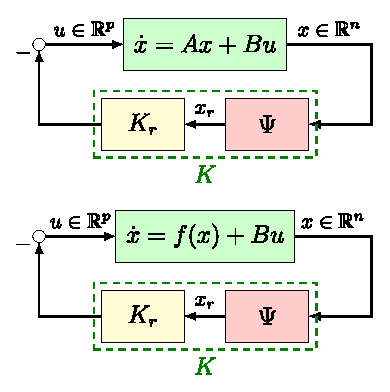
\includegraphics[width=0.6 \linewidth]{lqr_sketch}
\caption{Schematic of the implementation of the full-state feedback control in the full linear (top) and full non linear (bottom) simulations. The entire state is first projected onto the unstable eigenvectors and the stable subspace of the balanced modes in order to compute the reduced-order state $x_r$. The state is then multiplied by the gain $K$, computed based on the reduced-order model using $LQR$ to obtain the control input $u = - K_r   \Psi x $.}
\label{lqr_sketch}
\end{figure}


\subsection{Observer-based feedback control design}

In most engineering applications, the state of the full system is unknown, and thus a full-state feedback controller that updates the control input based on the the current state is not directly applicable. Instead, one typically uses an observer-based feedback controller to update the feedback control inputs based on the sensor measurements (outputs).

As before, using the reduced-order model, an observer is designed using a  quadratic estimator known as the Kalman filter. This method is optimal if the errors in representing the state $x_r$ and the measurements $y$ are stochastic Gaussian processes. Such errors typically arise from inaccuracies in the model, external disturbances, and sensor noise. The method gives us an estimate $\hat{x}_r$ of the state $x_r$ that is optimal in the sense that it minimizes the mean of the squared error; for more details, see \citet{Skogestad}.
\begin{figure}[htb]
\centering
  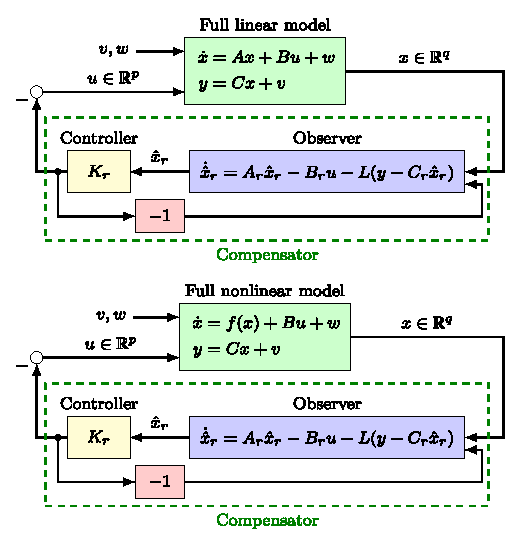
\includegraphics[width=0.8 \linewidth]{lqg1}
  \caption{Schematic of the implementation of the observer-based feedback control in the linear (top) and nonlinear (bottom) simulations. The control input $u$ and the sensor measurements y are used as inputs to the observer, which reconstruct the reduced-order state $\hat{x}_r$. This state is then multiplied by the gain $K_r$ to obtain the control input $u$. Both the controller and the observer gains $K_r$ and $L$ are computed based on the reduced-order model. }
\label{lqg1}
\end{figure}

The disturbances $w$ comes from the model truncation and ignoring the nonlinear terms in the reduced-order model (linearization). The sensor noise $v$ (error in measurements) comes from the output projection (the output is the projection of the approximated state onto the finite balanced truncation modes deduced previously).

The reduced-order model dynamics with process and sensor noise included is defined as follows:
\begin{equation}
\begin{aligned}
	\dot{x}_r &= {A}_r x_r  + {B}_r u +w,   \\
	y &= {C}_r x_r +v.
\end{aligned}
\end{equation}
Again, both disturbances and sensor noise are Gaussian processes whose variances are
\begin{subequations}
\begin{align}
Q &= E(ww^\dagger), \qquad w = P_{\rm bal} f(x) -  P_{\rm bal} {A} x \label{error1},   \\
R &= E(v v^\dagger),  \qquad \quad  v = y -  {C} P_{\rm bal} x \label{error2},
\end{align}
\end{subequations}
where $E(.)$ is the expected value, $P_{\rm bal}(.)$ is the projection onto the Balancing modes, $P_{\rm bal} = T_1 S_1$. The resulting estimator has the form
\begin{equation}
\begin{aligned}
	\dot{\hat{x}}_r &= {A}_r \hat{x}_r  - {B}_r u - L (y - {C}_r \hat{x}_r) ,   \\
	\hat{y} &= {C}_r x_r,
\end{aligned}
\end{equation}
where $\hat{y}$ is the estimated output and $L$ is the observer gain. The estimator is then used along with the full state feedback controller designed previously to determine the control input; a schematic is shown in Fig. \ref{lqg1}.

\section{Simulation Setup}
\label{Setup}

\subsection{Numerical parameters}
\label{num}
The nonlinear and linearized Hasegawa-Wakatani equations are solved in a two-dimensional slab geometry with doubly periodic boundary conditions for simplicity.

The grid size used is $16 \times 16$ with the computational domain given by $\left[ 0, L_x \right] \times \left[ 0 , L_y \right] $ and $L_x =L_y =22$, where lengths are normalized by $\rho_s$, the ion sound Larmor radius with $\rho_s \equiv v_{si} \omega_{ci}^{-1}$ where $v_{si} \equiv \sqrt{T_e/ m}$ is the ion sound velocity in the cold ion limit and $T_e$ is the electron temperature.

The time, ion vorticity and density fluctuation also have been normalized as follows:
\begin{equation}
\omega_{ci} t \mapsto t, \quad e \varphi/ T_e \mapsto \varphi, \quad n /n_0 \mapsto n, \quad x/ \rho_s
 \mapsto x.
 \end{equation}


\subsection{Input and output}
The system is actuated by a localized external electrostatic potential in the center of the slab. Its shape is given in Fig. \ref{actuator}. From Eq.~(\ref{init}), the initial condition used for each of the ion vorticity and density fluctuation simulations can be deduced. It is then shown in Fig. \ref{BB}.

The control objective is to prevent drift wave turbulence by stabilizing the unstable steady states of this model by using the unique actuator defined in Fig. \ref{actuator}, and designing a robust controller.
\begin{figure}[htb]
\centering
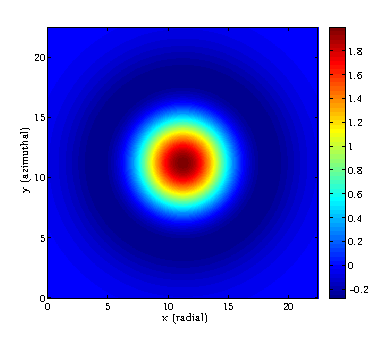
\includegraphics[width=0.7 \linewidth]{B1} 
\caption{Actuator localized at the middle of the square plate and modeled as a distribution of the external potential $\varphi_{ext}$ that is added to the system. It is determined by the function $f(r) = 2 \left(1-r^2/\gamma^2\right) \exp \left(-r^2/\gamma^2\right)$ where $r^2 =\left(x- L_x/2\right)^2 +\left(y- L_y/2\right)^2 $ and $\gamma = 5$ is a given parameter. }
\label{actuator}
\end{figure}
An example of a pair of unstable eigenvectors is shown in Fig. \ref{unstable eig}.
\begin{figure}[htb]
\centering
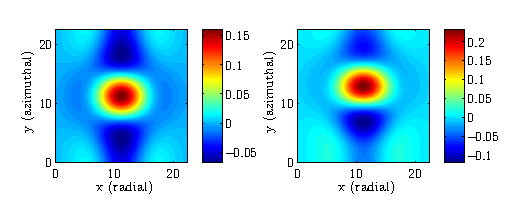
\includegraphics[width= \linewidth]{BB} 
\caption{(left) The ion vorticity $\zeta$ and (right) density fluctuations $n$ of the B-matrix defined in Eq.(14). These two quantities are going to be the initial conditions of the nonlinear, full linear, and reduced model of the MHW equations. }
\label{BB}
\end{figure}
\begin{figure}[htb]
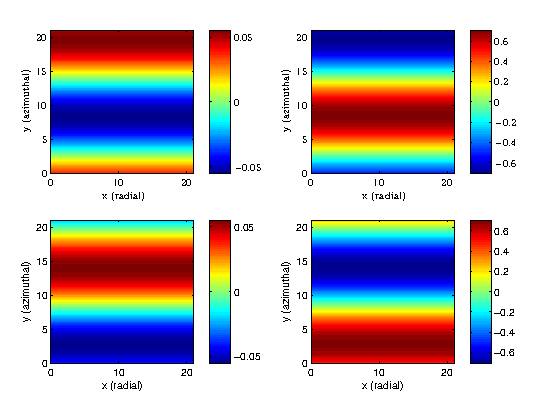
\includegraphics[width= \linewidth]{Tu}
  \caption{Representation of the two unstable eigenvectors of the linearized equations. The left part represents its real part, the right its imaginary part.}
  \label{unstable eig}
\end{figure}

Table~\ref{Tabparameter} summarizes the three numerical cases studied in the following section. Both $\alpha$ and $\mu$ values are fixed, the density gradient $\kappa$ is varied for each case, which gives us 3 different cases of right half plane (unstable) eigenvalues in the system.

\begin{table}[htbp]
\begin{center}
\caption{Summary of the 3 systems that will be reduced then stabilized  with only one actuator: for fixed $\alpha$ and $\mu$, only $\kappa$ is varied and obtain 3 different cases with 2, 4, or 8 right half plane (unstable) eigenvalues.}
\label{Tabparameter}
\begin{tabular}{ccccc}
Case& RHP poles & $\kappa$ & \makebox[5em]{$\alpha$}  & $\mu$  \\ \hline
1&2  &0.20 &0.1   & 0.2  \\
2& 4 & 0.25&  0.1  & 0.2   \\
3 & 8  & 0.28&   0.1 & 0.2  \\
\end{tabular}
\end{center}
\end{table}



\section{Results}
\label{Result}

The balanced truncation technique is applied to the MHW equations. In particular, a reduced-order model of the system is obtained, actuated by a localized external electrostatic potential in the center of the slab.

Using this reduced-order model, feedback controllers that stabilize its unstable steady states are developped; first, a full-state feedback controller is designed, then improved by developing a more realistic and practical observer-based controller that uses fewer measurements of the model to reconstruct the entire ion vorticity and density fields. 

The goal is to show that these well-known flow control techniques can be applied to this simplified plasma physics model, so that new methods for equilibria stabilization can be obtained, and savings of computational time and memory can be achieved. Those are very important especially in this domain, where computational requirements are typically large. 


\subsection{The nonlinear MHW equations }

The study begins by simulating the nonlinear MHW equations, in order to understand the fluctuations that are attempted to be stabilized.  The dynamics of coupled drift waves and zonal flows is found.

Figure \ref{movie nl ol} shows the transition of both ion vorticity and density fluctuation from a horizontally uniform state (drift waves) to an almost  vertically uniform state (zonal~flow);  the sequence then repeats.

 Figure \ref{output of nl} shows the same information about the density but focused on one point in the center of the grid, but for longer times, so the coupling between drift waves and zonal flow can be clearly seen  in terms of amplitude of one point of density fluctuation, but also in terms of the whole kinetic energy distribution.
\begin{figure}[htb]
\centering
  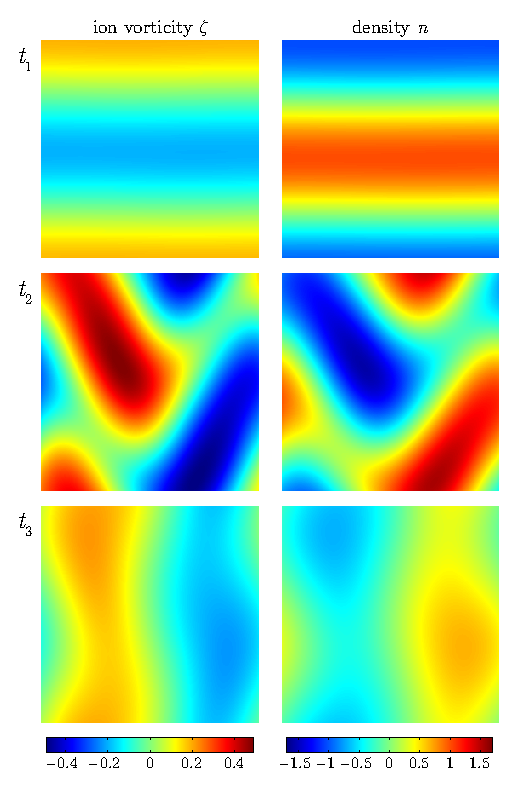
\includegraphics[width=0.7 \linewidth]{video}
  \caption{Ion vorticity and density fluctuation (in color) of the full non linear MHW equations at three successive times with the B-matrix as the initial condition. }
\label{movie nl ol}
\end{figure}

\begin{figure}[htb]
\centering
  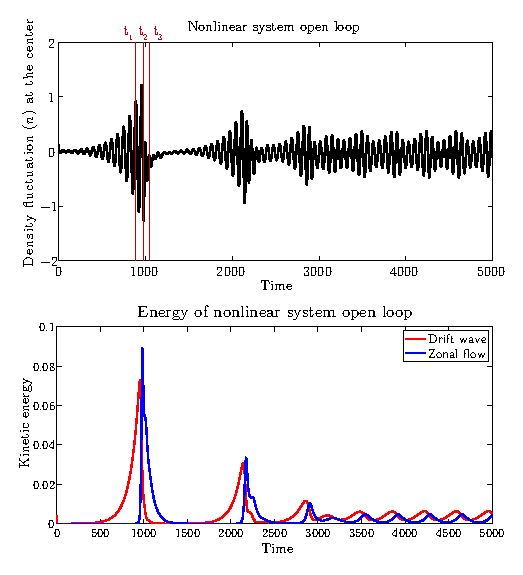
\includegraphics[width=0.7 \linewidth]{energy}
  \caption{The output correspond to the density fluctuation that occurs in the center of the square geometry with no control applied on the system. }
\label{output of nl}
\end{figure}


Having insights into the physics and understanding the coupling of drift waves and zonal flow can help to better design the controller. This idea will be discussed in Sec.~\ref{Conclusion}.
 
The aim of this paper is  not to explain the complex coupling between drift waves and zonal flow; the nonlinear simulation is only used to obtain a big picture of the phenomena in a particular case (here case 1 of Table~\ref{Tabparameter}), it will help to compare the model before and after applying the controller, and see whether a stabilization of these oscillations is possible near the unstable equilibrium.


\subsection{Reduced-order models and validation }
\label{ROMresults}

Once the balanced truncation is applied, the error between the original and the reduced-order model is calculated, and compared to its bounds (which were discussed in Sec.\ref{BT}), and to errors from POD and BPOD models (two other model reduction techniques seen in Sec.\ref{Spectrum}). 
The results are represented in Fig.\ref{error}.
As expected, the balanced truncation method is the one that gives the best approximation (least error) to the original model.

After validation, Table~\ref{Tabreduced} shows for the three studied cases, the new reduced dimensions obtained, once the balanced truncation is applied. These dimensions have significantly decreased. 

\begin{table}[htbp]
\begin{center}
\caption{Summary of the 3 new reduced systems. $r$ is the dimension of the stable reduced  subsystem.}
\label{Tabreduced}
\begin{tabular}{ccc} \hline
Case  &  \makebox[5em]{$r$} & Reduced dim. of state \\ \hline
1& 4&$512 \longmapsto 6$  \\
2 & 6& $512 \longmapsto 10$\\  
3  &12 & $512 \longmapsto 20$ \\
\end{tabular}
\end{center}
\end{table}


\begin{figure}[htb]
\centering
  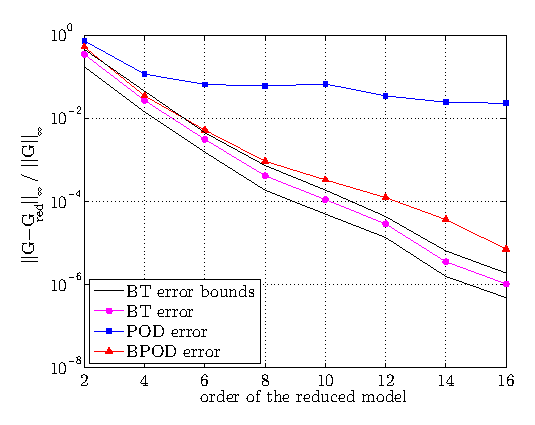
\includegraphics[width=0.7 \linewidth]{error}
  \caption{Error $||G-G_{red}||_{\infty} / ||G||_{\infty} $ for balanced truncation ($\bigcirc$), balanced POD ($\triangle$), POD ($\square$), and upper and lower bound for the model reduction scheme. }
  \label{error}
\end{figure}


\subsection{Full-state feedback control }
After designing a reduced-order model as described in Sec.~\ref{ROMresults}, a full-state feedback controller is then designed, in which it is assumed that vorticity and density can be measured everywhere.

The controller is built as in Sec.~\ref{Control}, using a LQR with $Q =  q * C^\dagger_r C_r$, and implementing it in the full linear system, as well as the full nonlinear system as shown in Fig.~\ref{lqr_sketch}.

By choosing $q \approx 10$ for the first case study in Table~\ref{Tabparameter}, the LQR is able to move the right half plane eigenvalues to the left without destabilizing the already stable left half plane ones. $q$ is chosen by numerically experimenting with different values, and then for each value, deduce the LQR controller and visualize the modified eigenvalues of the $ A_r-B_r K_r $ matrix. Thus, $q$ is chosen to be the best value that puts the right half plane eigenvalues of both the reduced and full linear models as far to the left as possible without destabilizing the other modes.

Figure \ref{lqr1} compares the density fluctuation in the center of the slab predicted by the reduced, full linear and non linear models  with inputs taken from the first case study defined in Table~\ref{Tabparameter} and Table~\ref{Tabreduced}. 

 At times $t<0$, the nonlinear system evolves freely without any control applied on it, the coupling effect is then observed while the reduced and full linear models exhibit just exponentially growing amplitudes that are not shown here. At time $t=0$, the controller is turned on and immediately for time $t>0$, the controller immediately damps the oscillations for all three systems, and their controlled dynamics become very close to each other. Therefore, the unstable steady state can be stabilized. More importantly, the reduced-order model predicts the outputs accurately when compared to the full linear or nonlinear system.


\begin{figure}[htb]
\centering
  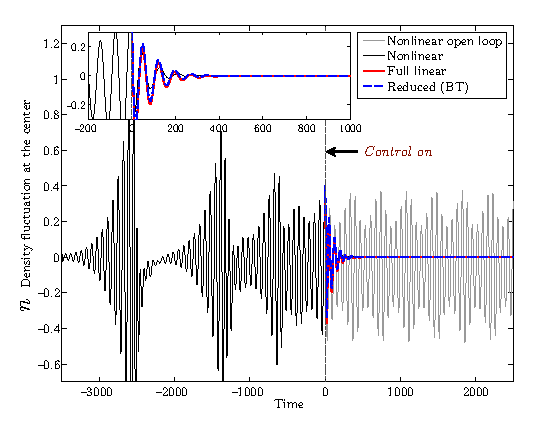
\includegraphics[width=0.7 \linewidth]{fullstate1}
  \caption{Full Linear model with 2 eigenvalues in the right half plane (RHP)}
  \label{lqr1}
\end{figure}

Figure \ref{lqr2} compares the density fluctuation in the center of the slab at two different controlling times with inputs taken from the second case study defined in Table~\ref{Tabparameter} and Table~\ref{Tabreduced}.

The nonlinear system evolves freely, and then at time $t=2000$, the controller is turned on (the output response is represented in red), the controller immediately damps the oscillations.
But when the controller is turned on at time $t=2300$, ( the output : density in the center, is represented in blue),  the controller is not able to damp the oscillations and stabilize the system due to the fact that it went too far from the attraction basin of the equilibrium point.

\begin{figure}[htb]
\centering
  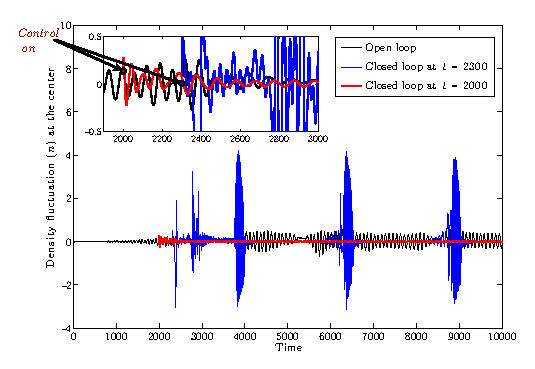
\includegraphics[width=0.7 \linewidth]{fullstate2}
  \caption{Full Linear model with 4 eigenvalues in the right half plane (RHP)}
  \label{lqr2}
\end{figure}

In order to see that, Fig.~\ref{lqr3}  (Top) shows the distance from the equilibrium for the 2 cases: the one inside the basin of attraction of the equilibrium point (control time at $t = 2000$) and the one outside the basin of attraction of the equilibrium point (control time at $t= 2300$). 
It can be seen that for the first case, the distance from the zero point tends to converge to zero, whereas in the second case, this distance keeps oscillating and diverges.
\begin{figure}[htb]
\centering
  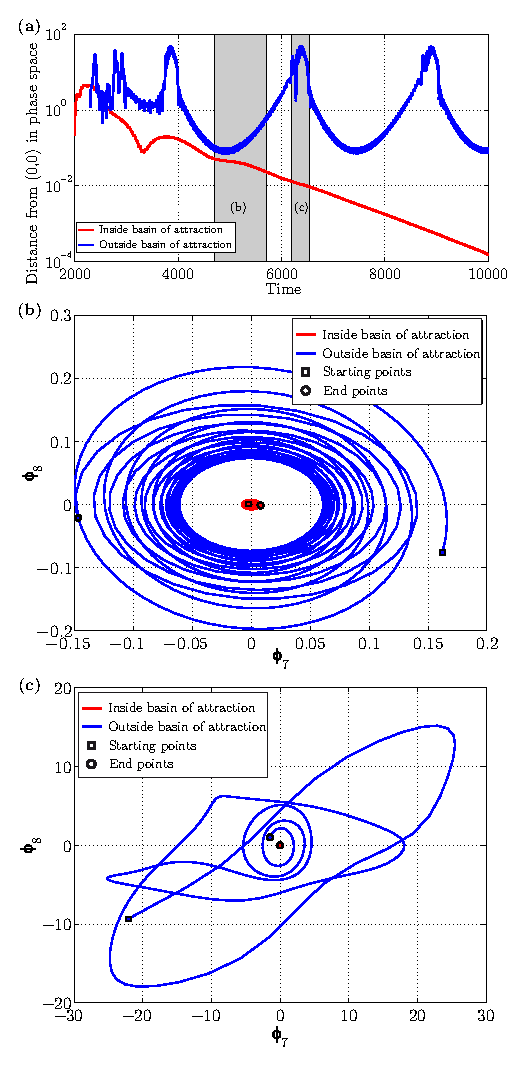
\includegraphics[width=0.7 \linewidth]{phase_space}
  \caption{Full Linear model with 4 eigenvalues in the right half plane (RHP): phase space plot}
  \label{lqr3}
\end{figure}

Figures \ref{lqr3} (middle and bottom) show the projection of the state on the 7th and 8th modes of the balanced truncation reduced-order model for two different time intervals indicated by the grey areas of the top figure and noted (B) and (C) respectively.
These two time intervals are chosen to illustrate when the solution is the closest and furthest of the equilibrium point respectively.

In (B) the stable solution is converging to the equilibrium point at $(0,0)$ whereas the unstable solution is initially approaching and then diverging from $(0,0)$.
In (C) the stable solution is still converging to $(0,0)$ whereas the unstable solution is following a complex path, sometimes being apparently close to the equilibrium point, but the projection on different modes would reveal that the distance is much larger.

For the controllable case, Fig.\ref{lqr6} shows a comparison of the reduced-order, full linear and nonlinear centered output of the system. Once again the oscillations are damped and stabilized and the dynamics of all three systems are approximately similar. This demonstrates that the reduced-order model is accurately predicting the full dynamics.
\begin{figure}[htb]
\centering
  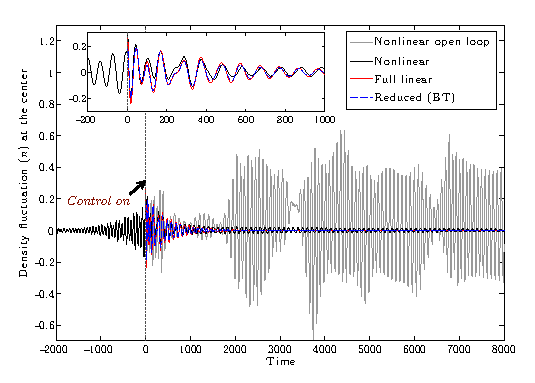
\includegraphics[width=0.7 \linewidth]{fullstate6}
  \caption{Full Linear model with 4 eigenvalues in the right half plane (RHP): inside basin of attraction case}
  \label{lqr6}
\end{figure}

Finally, as the parameter $\kappa$ increases to $0.28$, two more pairs of eigenvalues cross into the right-half plane (simultaneously).  One of these pairs turns out to be uncontrollable, as can be verified by the Popov-Belevitch-Hautus (PBH) test, \cite{Skogestad} so it is not possible to stabilize the equilibrium with this choice of actuation (shown in Fig.~\ref{BB}). 

\subsection{Observer-based feedback control}
In practice, the full-state feedback control of the system is not directly useful, since it is not possible to measure the entire ion vorticity and density fluctuation fields.
 Therefore considering a more practical approach; the reduced order models obtained from Sec. \ref{ROMresults} are used to design dynamic observers based on density fluctuation measurements at a small number of sensor locations. 
 
 A 6 (resp. 10) modes reduced order model with 2 (resp. 4) and 4 (resp.6) modes describing the dynamics on the unstable and stable subspaces respectively, is used to design the Kalman Filter for producing an optimal estimate of the density fluctuation and ion vorticity fields based on Gaussian approximations of error terms (\ref{error1}) and (\ref{error2}). This estimate is then used along with reduced order model controller to determine the control input as shown in Fig.~\ref{lqg1}. The results of this observer-based controller, which is also called a compensator, are shown for different sensors locations, in Figs. \ref{lqg2} and \ref{lqg3}.
 
Two cases of measurements are considered here:
\begin{itemize}
\item measurement of the whole density field, thus the $C$ matrix defined in Eq.~(\ref{linSS}) can be written as
\begin{equation}
C = [\begin{matrix}  0 & I \end{matrix}]
\end{equation}
\item measurement of only four points of the density field  as shown in Fig.[\ref{lqg4}] , thus the $C$ matrix can be written as
\begin{equation}
C = \left[ \begin{matrix}  0&  \dotsb 1 \dotsb &  & & & \\   & & \dotsb 1 \dotsb& &  \\  & & &  \dotsb 1 \dotsb& & \\ & & & & & \dotsb 1 \dotsb 0 \end{matrix} \right]
\end{equation}
\end{itemize}
Even though these sensors may not be realizable in applications, they serve as a reasonable testing ground for the models.
\begin{figure}[htb]
\centering
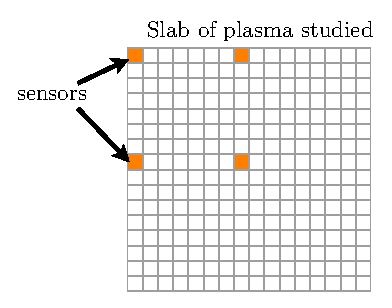
\includegraphics[width=0.65 \linewidth]{observer4}
\caption{sensors location}
\label{lqg4}
\end{figure}

Only the second case study results, which contains 4 RHP eigenvalues are shown here, as it contains some interesting constraints on special controlling times when it came about designing the Full state feedback.
The measurements will be done one time only  of the density field, the other time,  4 points of density only.

Figure \ref{lqg2} shows  a comparison of the outputs from the reduced-order, full linear, and nonlinear models when only the density field is measured. The oscillations are still damped and stabilized and the responses agree well, indicating that the reduced-order linear model is a good approximation to the full nonlinear system.
\begin{figure}[htb]
\centering
  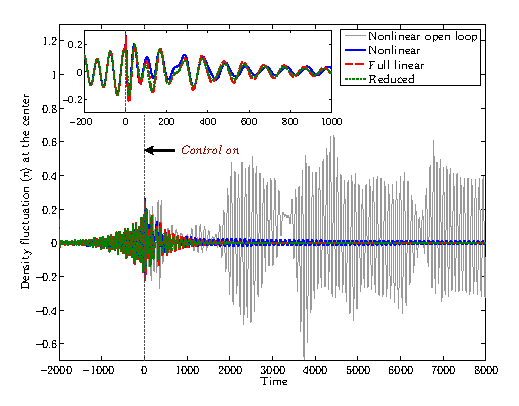
\includegraphics[width=0.7 \linewidth]{observer2} 
  \caption{Output feedback: 4 RHP poles/ Full density sensed }
  \label{lqg2}
\end{figure}

Figure \ref{lqg3} shows us a comparison of the outputs from the reduced-order, full linear and nonlinear models when only 4 density points are measured. The oscillations are damped and stabilized quicker for the linear models than the nonlinear model where it wiggles a little more and increases before converging to the equilibrium point. The dynamics of the 3 systems are approximately similar until a certain point (a transition behavior of the nonlinear system) but at the end, the controller will be able to control the nonlinear system with only 1 actuator and 4 sensors.

\begin{figure}[htb]
\centering
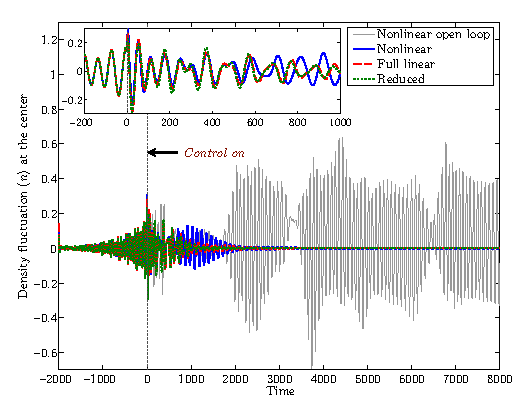
\includegraphics[width=0.7 \linewidth]{observer3} 
\caption{Output feedback: 4 RHP poles/ 4 density points sensed only}
\label{lqg3}
\end{figure}

The compensator again stabilizes the unstable equilibrium point and furthermore the observer reconstructs the reduced order model states accurately. Initially the observer has no information about the states ( the initial state estimate is $\hat x = 0$), but it quickly converges to and follows the actual states.

Finally to test the robustness of the resulting controller, a Nyquist \cite{Skogestad} plot of the loop gain of the input sensitivity function (input loop transfer function) is drawn for each unstable case (2 or 4 right half plane eigenvalues) which corresponds to Figs. (\ref{rob1}) and (\ref{rob2}) respectively. These plots show the loop transfer function for different outputs considered: measuring density and vorticity (full-state), measuring the full density field, and measuring density at four spatial locations.

 The gain (GM) and phase margins (PM) can be deduced from the plots and are given in Table~\ref{table3}. It indicates the amount by which the actual dynamics can differ from the model (either in gain or phase), before the closed-loop system loses stability.  The cases with only 4 sensors have very small stability margins, indicating that the model needs to be very accurate in order for the controllers to stabilize the equilibrium.
 
The small stability margins for the cases with only 4 sensors indicate that the controllers are unlikely to work in practice unless the model is very accurate.  However, the cases where the full density field is known are.

 More details about the tools and theory behind it can be found in \citet{Astrom}
 
\begin{figure}[htb]
\centering
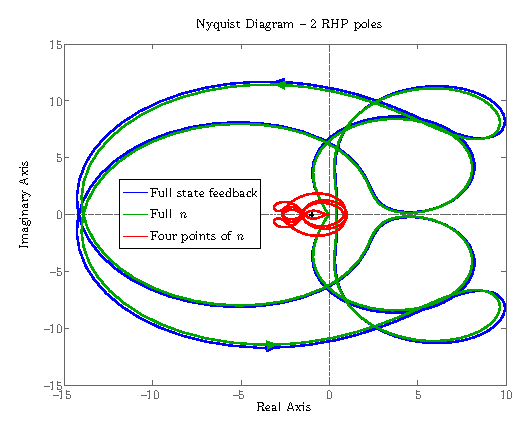
\includegraphics[width=0.67 \linewidth]{robust1}
\caption{Nyquist diagram of the loop gain of the input sensitivity function for the unstable case with two right half plane eigenvalues.}
  \label{rob1}
\end{figure}

\begin{figure}[htb]
\centering
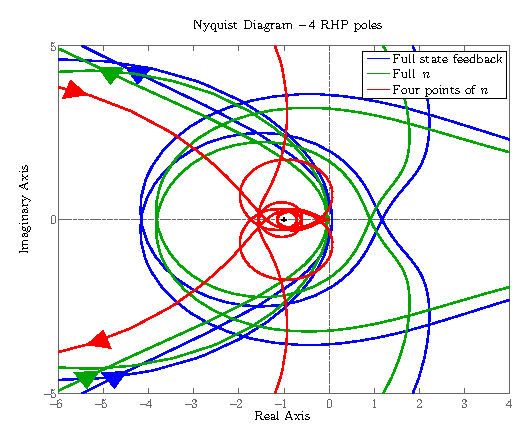
\includegraphics[width=0.67 \linewidth]{robust2}
\caption{Nyquist diagram of the loop gain of the input sensitivity function for the unstable case with four right half plane eigenvalues.}
  \label{rob2}
\end{figure}


\begin{table}[htbp]
	\caption{GM and PM deduced from the loop gain of the sensitivity function}
	\label{table3}
	\begin{tabular}{|c|c|c|c|} \hline
		Case & num. of sensors & Gain Margin & Phase Margin \\ \hline
		1 pair of  & 512&82.2&$56.6^\circ$   \\ 
		RHP e-values  & 256& 41.3&$56 ^\circ $\\ 
		  &4 & 1.26& $11.8^\circ$ \\ \hline
		2 pairs of  &512 &19.3 &$54.3^\circ$ \\ 
		RHP e-values  &256 & 13.5& $53^\circ$ \\ 
		  &4 & 1.32& $13.9^\circ$\\ \hline
	\end{tabular}
\end{table}

\clearpage

\section{Summary and discussion}
 \label{Conclusion}
 The numerical methods for developing a reduced-order model of the input-output dynamics of linear unstable systems are briefly presented in this paper. It is assumed for simplicity that the dimension of the unstable eigenspace is small and the corresponding global modes can be numerically computed. Building the reduced order model treats the unstable subspace exactly, and truncates from the stable subspace only.
 
These techniques have been frequently used in fluid control community.  The aim of this work has been to introduce and extend these methods to the plasma physics community. Stabilizing controllers based on the reduced-order linear models were developed and applied on unstable state and it was showed that when it works, the models obtained agreed well with the actual simulations.These linear controllers applied to the full nonlinear simulations were fairly successful at suppressing the drift wave turbulence.

A 10 modes reduced-order observer which reconstructed the density and vorticity fields accurately was designed along with an optimal controller, and was able to suppress the drift wave turbulence and stabilize the two fields in the neighborhood of the equilibrium point.

Even if the actuator and sensors considered here are not practically realizable, the methodology presented can be extended to a more practical actuation. If given a different equilibrium point than zero, using and amplifying the zonal flow as an actuation would be a smart choice because of its stabilizing effects; once actuated, the zonal flow can reduce the drift wave turbulence as seen in Figs.~\ref{movie nl ol} and \ref{output of nl}. This actuation may be a more physical particular way of actuating the plasma slab for this special case where it has an attenuation effect.

Also, adding more actuators and improving their design will provide better control. Here, the whole study was done with only one actuator and in some cases, the stabilization of the whole density and vorticity fields was possible with this unique actuator.

Furthermore, the choice of sensor locations was not optimal either for the given actuator, and different choices for sensor measurements could lead to improved performance. 

Finally, a motivation for the choice of this model problem was to show all the possibilities of these control design techniques for a simple model. In the future, for more realistic tokamak models, it may help to make the entire stabilization procedure more automated and rigorous.\\\\
%
This work was supported by the U.S. Department of Energy Grant under Contract No. DEAC02-76CH03073.


\chapter{Modeling and control of plasma rotation for NSTX using Neoclassical Toroidal Viscosity and Neutral Beam Injection}
\label{rot1&}

\textbf{\large I. R Goumiri$^1$, C. W. Rowley$^1$, S. A. Sabbagh$^2$, D. A. Gates$^3$, S. P. Gerhardt$^3$, M. D. Boyer$^3$, R. Andre$^3$ E. Kolemen$^3$ and K. Taira$^4$} \\
{\footnotesize $^1$ Dept. of Mechanical and Aerospace Engineering, Princeton University, Princeton, NJ 08544, USA \\[-0.1em]
$^2$ Department of Appl. Physics, Columbia University, New York, NY 10027, USA \\[-0.1em]
$^3$ Princeton Plasma Physics Laboratory, Princeton, NJ 08544, USA \\[-0.4em] $^4$ Florida Center for Adv. Propulsion, Florida State University, Tallahassee, Florida 32310, USA \\[1em]}
%
{\footnotesize Appears in Journal of Nuclear Fusion,56 036023, (2016) . \href{http://dx.doi.org/10.1063/1.4796190}{doi:10.1088/0029-5515/56/3/036023}} \\[0.5em]

\noindent
A model-based feedback system is presented to control plasma rotation in a
magnetically confined toroidal fusion device, to maintain plasma stability for
long-pulse operation.
%
This research uses experimental measurements from the National Spherical Torus
Experiment (NSTX) and is aimed at controlling plasma rotation using two
different types of actuation: momentum
from injected neutral beams and neoclassical toroidal viscosity generated by
three-dimensional applied magnetic fields.
%
Based on the data-driven model obtained, a feedback controller is designed, and
predictive simulations using the TRANSP plasma transport code show that the
controller is able to attain desired plasma rotation profiles given practical
constraints on the actuators and the available measurements of rotation.\\

\hrule

\section{Introduction}

Spherical tokamaks such as the National Spherical Torus Experiment (NSTX
\cite{Ono00}) are toroidal magnetic fusion devices that have been proven
experimentally to realize theoretical expectations of efficient and compact
advanced tokamak operation, producing high plasma pressures in relation to the
pressure of the magnetic field used to create the plasma equilibrium. In certain
circumstances, these high pressures can cause rapidly growing
magnetohydrodynamic (MHD) plasma instabilities that can lead to undesirable
effects such as reducing the plasma pressure, or even terminating the plasma (disruption).
%
Many of these instabilities are sensitive to the shear, so the rotation profile
plays a key role in regulating these instabilities.
%
The goal of the present study is to describe a model-based approach to
controlling the rotation profile in spherical tokamaks, and to apply the
approach to a predictive model based on experimental data from NSTX.

The effect of the rotation profile on MHD instabilities has been well studied in
recent years.  For instance, greater stability of tearing modes has been associated with
increased rotation shear \cite{Gerhardt09, Park13}, while
rotation profile shapes that lead to stronger kinetic resonances lead to
stabilization of kink/ballooning modes and resistive wall modes \cite{Sabbagh10,
  Berkery10}. Furthermore, rotational shear can affect plasma turbulence and
consequently can have an impact on transport processes and the energy
confinement performance of tokamak plasmas \cite{Biglari90, Terry00, Hahm94}. In present-day pulsed tokamaks,
plasma rotation can evolve, through normal heat and momentum transport
processes, toward profiles for which certain MHD modes are unstable.
%
Even if these profiles evolve by chance to a steady-state profile that is
stable, transient processes including Edge-Localized Modes (ELMs), internal transport
barriers, and different heating mechanisms can alter plasma profiles further and make
them less stable, or unstable \cite{Sabbagh13}.
%
In future large fusion-power-producing tokamak operation (e.g. the fusion nuclear science facility, FNSF
\cite{Peng05, Peng11, Peng09}), disruptions caused by macroscopic instabilities can generate
electromagnetic forces and heat loads large enough to damage device components,
so it is particularly important to avoid such disruptions, for instance through
control of the rotation profile.

There is an abundant literature on plasma control such as kinetic profile control (density and temperature) \cite{Schuster02, Boyer11}, burn control \cite{Schuster01, Schuster02-2, Schuster02-3, Vitela98, Boyer12}, toroidal current profile control \cite{Boyer133, Boyer144, Barton12, Ou09, Ebrahimi04},  safety factor profile control \cite{Argomedo13, Maljaars15, Kim12},  direct control of tearing modes \cite{Welander13, Volpe09} and resistive wall modes \cite{Sabbagh06,Sabbagh13}. Rotation control in tokamaks has been demonstrated using momentum input from injected neutral beams (NBI) as an actuator \cite{Scoville07, Yoshida09}.  A new and unique aspect of the present work is the use of non-axisymmetric (three-dimensional) magnetic fields as another actuator in closed-loop feedback control to supplement the neutral beam actuator. Rotation alteration by non-resonant, three-dimensional magnetic fields allows more precise, continuous control of the plasma rotation alteration than NBI, as the momentum delivered by the latter occurs in significantly large, discrete increments.

The physical process creating the force on the plasma rotation generated by the applied three-dimensional field, termed neoclassical toroidal viscosity (NTV) \cite{Shaing88, Shaing10, Shaing15}, has been used successfully to affect plasma rotation in a pre-programmed manner on NSTX over a wide range of plasma operation, with quantitative agreement of the experimentally generated torque to theory \cite{Zhu06}. NTV is caused by non-ambipolar diffusion of plasma ions and electrons caused by the magnetic field components that break the usual toroidal symmetry of tokamak confinement field. As NTV depends on several important plasma parameters including temperature, and the plasma rotation itself, its use in closed-loop feedback leads to weak nonlinearities which must be investigated to ensure successful control. Details of such elements will be shown throughout this work. 

The present work defines a model-based algorithm for plasma rotation control
based on experimental data from NSTX \cite{Ono00}, that measures the rotational
(toroidal) momentum transport in the tokamak.
More details about how to measure rotation profile in real-time can be found in \cite{Zhu06, Podesta12}.
Data-driven modeling techniques
have been successfully used in the past to model plasma transport dynamics for
active control design in fusion reactors \cite{Moreau13, Boyer133, Boyer144,
  Barton12}. A novel contribution of this work is the development of a
one-dimensional partial differential equation model that is computationally
inexpensive, and may therefore implemented for real-time control.
%
The present simplified model of plasma momentum transport retains the most
important elements of the plasma momentum balance, including the effects of NBI
and NTV, and reproduces the general features of the plasma rotation evolution
measured in experiments.

Once the model is satisfactorily developed, a further step consists of applying
a spectral decomposition method, linearizing the equation about an equilibrium
and projecting onto a subspace spanned by Bessel functions, in order to obtain
an approximate linear model consisting of just 5 ordinary differential
equations.
%
The resulting reduced model is then used to design a controller using standard
techniques from optimal control.
%
The advantage of using a reduced-order model is that the resulting controller is
also low dimensional, so that it is computable in real time, as well as being
easier to tune and design.
 
The paper is organized as follows.  Section~\ref{MHW} describes the data-driven model
definition with details about the actuators used, model reduction process and
comparison to experimental data. Section~\ref{LRPC} describes the optimal
control method used to track a desired rotation profile, using both NTV and NBI
as actuators, and its implementation through numerical simulation. Section~\ref{sec:sim_results}
presents the results of the designed controller on a more complete rotation
model that can be found in TRANSP, a time dependent code developed at Princeton
Plasma Physics Laboratory for both prediction and analysis of tokamak
experimental data \cite{Goldston81, Budny94}. Conclusions and future work are
discussed in Section~\ref{sec:conclusions}.


 \section{A simplified model of  the toroidal momentum balance }
 \label{MHW}
 
\subsection{Model definition}
Consider the transport of toroidal angular plasma momentum in a tokamak with the assumption of axisymmetry.  To facilitate the analysis, an arbitrary flux surface average $\rho \in [0,1]$ is used, where $\rho = 0$ and $1$ denote the center and the boundary of the plasma, respectively.  

Using the work of Goldston \cite{Goldston86}  and Callen  \cite{Callen09}, the angular velocity of the plasma $\omega$ can be described dynamically by the flux surface average $\left<\cdot\right>$ of the toroidal momentum equation 
\begin{multline}
  \sum_i n_i m_i \left<R^2\right> \frac{\partial \omega}{\partial t}
  + \omega \left<R^2\right> \sum_i m_i \frac{\partial n_i}{\partial t} 
  + \sum_i n_i m_i \omega \frac{\partial \left<R^2\right>}{\partial t} \\
  + \sum_i n_i m_i \left<R^2\right> \omega \left( \frac{\partial V}{\partial\rho}\right)^{-1} \frac{\partial}{\partial t} \frac{\partial V}{\partial \rho} \\
  = \left( \frac{\partial V}{\partial\rho}\right)^{-1}\frac{\partial}{\partial \rho} \left[\frac{\partial V}{\partial \rho}\sum_i n_i m_i \chi_\phi \left< R^2 (\nabla \rho)^2\right> \frac{\partial\omega}{\partial\rho}\right] \\
  - \left( \frac{\partial V}{\partial\rho}\right)^{-1}\frac{\partial}{\partial \rho} \left[\frac{\partial V}{\partial \rho}\sum_i n_i m_i \omega \left< R^2 (\nabla \rho)^2\right> \frac{v_\rho}{|\nabla\rho|}\right] \\
  - \sum_i n_i m_i \left< R^2\right> \omega \left( \frac{1}{\tau_{\phi cx}} + \frac{1}{\tau_{c\delta}}\right) + \sum_j T_j.
	\label{eq:full1}
\end{multline}
The left-hand side of the equation above represents the temporal change in the plasma toroidal angular momentum and the right-hand side terms denote respectively the one-dimensional fluid viscous term, pinch term, momentum loss due to charge exchange and field ripple, and the torque inputs (i.e., neutral beam injection and neoclassical toroidal viscosity). $R$ is a major radial coordinate, $\partial V/\partial\rho$ is the differential flux surface volume, $\chi_\phi$ is the perpendicular (to the equilibrium magnetic field) momentum diffusivity, $\tau_{\phi c x}$ and $\tau_{c\delta}$ are the time scales of the local momentum loss associated with charge-exchange and field ripple, $T_j$ represents the various torques acting on the system, $n_i$ is the particle density and $m_i$ is the particle mass for each particle species, but for simplicity, only the main plasma ion species (deuterium) are considered in the dynamics.

It is assumed that the plasma cross-sectional shape is well controlled by a
separate control loop; therefore $\left< R^2 \right>$, $\left< R^2
  (\nabla\rho)^2 \right>$, and $\partial V/\partial \rho$ are held fixed.
Curve-fits from time-averaged values of these functions (4th (Figures~\ref{fig:geofunc}(\emph{a}) and (\emph{c})), 5th (Figures~\ref{fig:geofunc}(\emph{b}) and (\emph{d})) order
polynomials or cubic spline (Figure~{\ref{fig:chiphi}}) interpolation depending on which one gives the smoothest fit) from TRANSP analysis of an experimental
plasma are used as approximations.
%
Representative data for a plasma discharge (133367) is shown in
Figures~\ref{fig:geofunc}(\emph{a}), \ref{fig:geofunc}(\emph{b}) and
\ref{fig:geofunc}(\emph{c}) respectively.  As it can be seen, the temporal
fluctuations of these variables are small. Hence taking the time-average values
or even the fixed values at an adequately chosen time ($t = 0.65 s$) is
considered to be a close approximation.
%
\begin{figure}
\centering 
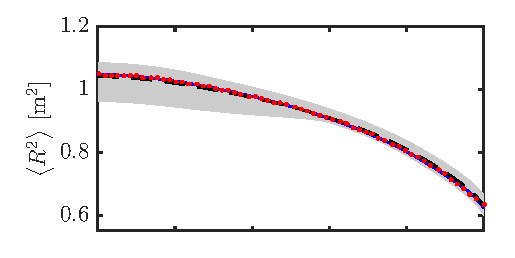
\includegraphics{fig1a} \hspace{-3em}\raisebox{7.7em}{(a)} \\
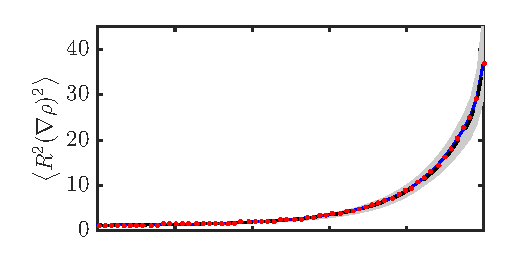
\includegraphics{fig1b} \hspace{-3em}\raisebox{7.7em}{(b)} \\
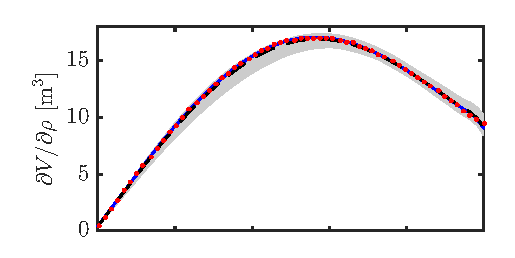
\includegraphics{fig1c} \hspace{-3em}\raisebox{7.7em}{(c)} \\[-.4em]
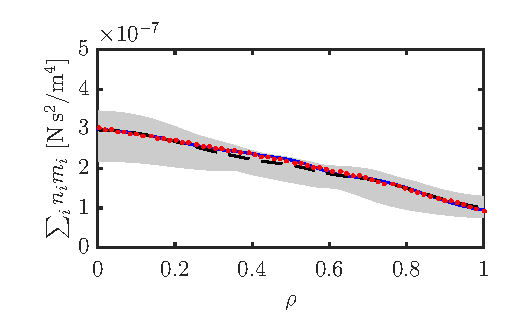
\includegraphics{fig1d} \hspace{-3em}\raisebox{9.7em}{(d)}
\caption{Functions describing the radial profiles of the geometrical properties: $\left< R^2 \right>$, $\left< R^2 (\nabla\rho)^2 \right>$, $\partial V/\partial \rho$ and  the mass density $ \sum_i n_i m_i $ from a TRANSP analysis of plasma discharge 133367.  The shaded region represents the value of the function spanned over time interval ($0.45$--$0.92$) seconds. The time-average values are shown by the black dashed line (--~--), the fixed time values and its curve-fit are shown by the solid blue lines (---) and the red dots (o) respectively.}
\label{fig:geofunc}
\end{figure}

It is also assumed for simplicity that the time variation of the mass density is
small.  This is a reasonable approximation, especially towards the edge ($\rho=1$), as seen in Figure~{\ref{fig:geofunc}}(\emph{d}).
This assumption may later be removed allowing $ \sum_i n_i m_i $  to vary in
time for more complex time-dependent systems, but for now, it allows the density
time derivative term in the left-hand side of equation~(\ref{eq:full1}) to be
neglected, resulting in a time-invariant system that is more amenable to control
design.
 
 Incorporating these observations into equation~(\ref{eq:full1}), we obtain a simplified diffusion equation
\begin{multline}
 n m \left<R^2\right>
 \frac{\partial \omega}{\partial t} 
 = \left( \frac{\partial V}{\partial\rho}\right)^{-1}
   \frac{\partial}{\partial \rho} 
   \left[\frac{\partial V}{\partial \rho} n m \chi_\phi 
   \left< R^2 (\nabla \rho)^2\right> 
   \frac{\partial\omega}{\partial\rho}\right] + T_\text{NBI} + T_\text{ NTV},
		\label{model0}
\end{multline}
with boundary conditions
\begin{equation}
\left.\frac{\partial\omega}{\partial\rho}\right|_{\rho=0} = 0 
\quad \text{and} \quad 
\left.\omega\right|_{\rho=1} = 0.
\label{bc0}
\end{equation}
Here, $T_\text{NBI} $ and $T_\text{NTV}$ represent the torques
arising from neutral beam injection (NBI) and neoclassical toroidal viscosity
(NTV). Note that for this significant class of high confinement discharges specific to NSTX, the
pinch term and  the momentum loss due to charge exchange are small \cite{Solomon08, Kaye09} and the
momentum loss due to  field ripple is not required, as NTV is explicitly
determined in this calculation. Details of the models for $T_\text{NBI}$
and~$T_\text{NTV}$ are shown in Sections~\ref{NBIAM} and~\ref{TNTV}.  The
Dirichlet boundary condition at the plasma edge ($\rho=1$) is chosen to be
consistent with experimental observations.
  
A few observations can be made about this simplified model: first, equation  (\ref{model0}) is parabolic, ensuring the state operator to be negative definite (all eigenvalues are negative);  hence the system is stable, which is a desirable feature from a control viewpoint. 
Second, this approach captures only the momentum balance for rotation control and does not model potential plasma instabilities.
  
A key parameter in the model is the diffusion coefficient $\chi_\phi$, which we
take to be constant in time in~(\ref{model0}).
There are no direct measurements of $\chi_\phi$ inside the tokamak, but TRANSP
is able to reconstruct a value for $\chi_\phi$ for an experiment where $\omega$
is measured.
%
Figure~{\ref{fig:chiphi}} shows the deduced $\chi_\phi$ from a particular run (plasma discharge number~133775). This run is identical to the plasma discharge number~133367 except that it does not have an applied non-axisymmetric field, and therefore $T_\text{NTV} = 0$. This feature is very important because each dissipation effect needs to be considered separately from each source in the model. The data driven model will use the $\chi_\phi$ of discharge (133775) as its momentum diffusivity coefficient reference.


\begin{figure}
\centering
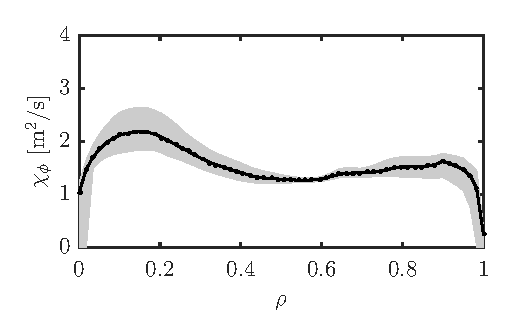
\includegraphics{fig2}
\caption{The momentum diffusivity coefficient $ \chi_{\phi}$ is calculated through TRANSP analysis of plasma discharge 133775.  The shaded region represents the value of the function spanned over time interval ($0.45$--$0.92$) seconds. The time-average values and its curve-fit are shown by the circles  and the solid line respectively.}
\label{fig:chiphi}
\end{figure}


The approach here is as follows: given a range of desired profiles that
the operator wishes the system to reach and stabilize,
take the simplified model~(\ref{model0}) that relies on different models of $ n  m$,
NTV and NBI torques from a representative class of plasma discharge ($\chi_\phi$ modeled from plasma discharge 133775),
linearize the model around an equilibrium whose basin of attraction contains the range of desired profiles
and use the linearized model to design a controller that will attempt to match any target shape within this range.

\subsection{Actuator models}

In order to control the toroidal momentum of the plasma in a spherical tokamak, we consider the use of two actuator mechanisms, namely, the neutral beam injection (NBI) and the neoclassical toroidal viscosity (NTV). The neutral beams are the main sources of momentum for the plasma and the NTV actuator is primarily used as a source of drag on the plasma. For NSTX, $T_\text{NBI}$ is strongest  in the plasma core, whereas $T_\text{ NTV}$ is strongest closer to the edge of the plasma. The momentum diffusivity $\chi_\phi$ allows transport of the momentum across these plasma regions on the momentum diffusion timescale of about $0.1\,s$ in NSTX H-mode plasmas.


\subsubsection{Neutral Beam Injection (NBI)}
 \label{NBIAM}

In NSTX, neutral beam injection is the main method to produce positive torque to increase plasma rotation, which is achieved  by injecting high-speed neutral atoms into the center of the plasma. 
Neutral atoms are able to cross the confining magnetic field of the tokamak without being deflected, and are ionized in the plasma via collisions with ions and electrons. The fast ions that are generated are also confined in the magnetic field and are able to exchange their energy to plasma ions and electrons. Typical injection acceleration voltages are in the range of 50\,keV to 130\,keV and for comparison, in NSTX, the peak plasma ion thermal temperature reaches up to $1.5$ keV.
Figure~{\ref{NBI_pics}} shows the planned neutral beam injection for the present
upgrade of NSTX. In the present study, we consider the three neutral beam
sources injected from the injector shown on the left of the figure.
Furthermore, for simplicity, we model the three sources as a single torque
input, as we describe below.

\begin{figure}
\centering
\begin{tabular}{cc}
\includegraphics[width=0.7 \linewidth]{fig3a} \\
\includegraphics[width=0.7\linewidth]{fig3b}
\end{tabular}
\caption{Illustration of the neutral beam injection (NBI) devices for NSTX-U with an inside view from the top of the tokamak (top) and outside view (bottom).}
\label{NBI_pics}
\end{figure}


A differential-equation model is introduced to relate the input power to the generated torque.  First, we approximate the NBI torque as a product of the spatial average of the torque, $\overline{T}_\text{NBI}(t) \equiv \text{avg}_\rho T_\text{NBI}(t,\rho)$, and a function, $F_\text{NBI}(\rho)$, that represents the spatial profile
\begin{equation}
   T_\text{NBI}(t,\rho) = \overline{T}_\text{NBI}(t) F_\text{NBI}(\rho),
\label{eq5}
\end{equation}
where the spatial profile of the torque is taken to be a Gaussian function (based on TRANSP analysis of NSTX discharge 133367) written as
\begin{equation}
F_\text{NBI}(\rho) = a_\text{NBI} \exp\left( - \frac{\rho^2}{2\sigma^2_\text{NBI}}\right).
\label{eq6}
\end{equation}
%
\begin{figure}
\includegraphics[width=0.47 \linewidth]{fig4a} \hspace{-2.7em}\raisebox{6.2em}{(a)}\hspace{2em}
\includegraphics[width=0.47 \linewidth]{fig4b} \hspace{-2.7em}\raisebox{4.2em}{(b)}
\caption{(a) Spatial profile for the neutral beam torque ($F_\text{NBI} $) for
  plasma discharge 133367.  The shaded region represents the values for times
  ranging from 0.45 to 0.92~seconds: time averaged values (--~--); values at the
  fixed time $t=0.6$s  (\textcolor{blue}{--~$\cdot$}); and
  the fit~\eqref{eq6} (\textcolor{red}{---}).
  %
  (b) Spatial average of the torque generated for the same plasma discharge
  ($ \overline{T}_\text{NBI}$), showing the TRANSP analysis
  (black) and the model~\eqref{eq:nbi_time} (red),
  %
  with
  $\tau_\text{NBI} = 0.01\,\text{s}$ and  $\kappa_\text{NBI} =
  2\times10^{-6} $.}
\label{fig:Fnbi}
\end{figure}
%
Figure~{\ref{fig:Fnbi}}(\emph{a}) shows the deduced profile $F_\text{NBI}$ of
the torque generated by the neutral beams, where the parameters
$a_\text{NBI}= 7.9090$
and~$\sigma_\text{NBI}= 0.2219$ were determined by a least-squares fit to the
time-averaged data.

In our model, the spatial average of the torque $\overline{T}_\text{NBI}(t)$ is
related to the power input, $P_\text{NBI}(t)$, by a first-order lag:
%
\begin{equation}
   \frac{\partial \overline{T}_\text{NBI}}{\partial t}
   + \frac{\overline{T}_\text{NBI}}{\tau_\text{NBI}}  = \kappa_\text{NBI} P_\text{NBI}(t),
   \label{eq:nbi_time}
\end{equation}
%
where $\tau_\text{NBI}$ is the approximate slowing down time of the fast neutral
beam particles to impart energy to the bulk plasma and $\kappa_\text{NBI}$ is a
scalar used to normalize the neutral beam power $P_\text{NBI}$.
%
$\tau_\text{NBI}$ depends on the collisionality and can affect the response time of the beam power actuator.
For values of $\tau_\text{NBI}$ between 10 and 30ms, the impact that the actuator has on the control does not change significantly.
By fitting equation~\eqref{eq:nbi_time} with TRANSP analysis of Figure~\ref{fig:Fnbi}(b),
$\tau_\text{NBI}$ is set to $0.01$s.

Figure~\ref{fig:Fnbi}(\emph{b}) shows the solution of
equation~(\ref{eq:nbi_time}) with $P_\text{NBI}$ fixed to 6\,MW, compared with
the neutral beam torque predicted by TRANSP analysis, which uses a more
elaborate Monte Carlo model.


\subsubsection{Neoclassical Toroidal Viscosity (NTV)}
 \label{TNTV}

Tokamaks usually have error fields or magnetohydrodynamic (MHD) activities present and these imperfections break the toroidal symmetry of the magnetic field and result in enhanced neoclassical toroidal plasma viscosity which then increases the rate of toroidal flow damping. The result will be a change of the edge rotation and shear. 

\begin{figure}
\centering
\includegraphics[width=0.47 \linewidth]{fig5}
\caption{Model representation of the three-dimensional coils (highlighted in
  blue) used to create the magnetic field that produces NTV in the NSTX device.}
  \label{pic_NTV}
\end{figure}
For the current one-dimensional toroidal momentum model, we aim to model the momentum loss due to the neoclassical toroidal viscosity in the toroidal average sense and base our model on the work done in \cite{Zhu06} from which we can design the NTV torque as the bilinear product of the coil (Figure~\ref{pic_NTV}) current squared ($ I^2$) with the toroidal momentum $\omega$ as follows
\begin{equation}
   T_\text{NTV}  (t, \rho) =  - K \, G(\rho) \,  \langle R^2 \rangle \:  I^2(t) \,\omega (t, \rho),
    \label{eqn:ntv}
\end{equation}
where $K$ is a constant and $G$ is a Gaussian function.
\begin{figure}
\centering
\includegraphics[width=0.7 \linewidth]{fig6} \adjustbox{raise=10.2em, lap=-16em}{} % current
\caption{ Coil current $I(t)$ for plasma discharges 133367:
the green line represents the model from CHERS data and  blue lines represent the smoothed data.}
\label{fig:current}
\end{figure}
The present model  will focus on the torque generated by the $n=3$ applied field ``configuration,'' in which the current reverses direction in each of the six neighboring coils. Other applied field configurations are possible (e.g., configurations with dominant $n = 2$ component) and have experimentally produced effective NTV as well \cite{Sabbagh10}.
 
The approach in our model is to approximate the general shape of $T_\text{NTV}/\omega$ by a time-invariant spatial profile and a time-evolution of a scalar current, similar to the way $T_{NBI}$ was treated. The resulting model has the form  
\begin{equation}
   \frac{T_\text{NTV}(t,\rho)}{\omega(t,\rho)} = - G_\text{NTV}  (\rho) \, I^2(t),
\end{equation}
where
\begin{equation}
G_\text{NTV}  (\rho) = K \,  \langle R^2 \rangle \:G(\rho),
\end{equation}
%
\begin{figure}
\centering
\includegraphics[width=0.7 \linewidth]{fig7}
\caption{3D representation of the NTV torque model~\eqref{eqn:ntv} where
  $\omega$ is taken from experimental measurements of ``fixed'' plasma discharge
  133367, and $I^2$ is as shown in Figure~\ref{fig:current}.}
\label{TNTV3D}
\end{figure}
%
and $G(\rho)$ is a Gaussian function centered towards the edge ($\mu =0.7, \sigma =0.1$).
%
Figure~{\ref{fig:current}} shows the current that flows into the coils
for the plasma discharge 133367. We notice that the current is kept constant
after $0.6$s. It should be noted that for control design, the actuator input
will be~$I^2(t)$.
%
Using the experimental rotation profile, the modeled NTV torque is shown in Figure~\ref{TNTV3D}.

\subsection{Testing and comparing the model}
\label{sec:test-comp-model}
\subsubsection{Discretization of the model}
In order to numerically simulate the partial differential equation~\eqref{model0}, we use a spectral method, projecting onto suitably chosen basis functions, to obtain a system of ordinary differential equations.  In particular, we write
\begin{equation}
\omega(\rho,t)  = \sum_{n=1}^{N} a_n(t) \varphi_n(\rho),
\label{decomp}
\end{equation}
where the basis functions are given by
\begin{equation}
  \label{eq:1}
  \varphi_n(\rho) = J_0(k_n\rho),\qquad n=1,\ldots,N,
\end{equation}
where $J_0$ denotes the Bessel function of the first kind and $k_n$ denotes the $n$-th root of $J_0$.  With this choice of basis functions, the expansion~\eqref{decomp} automatically satisfies the boundary conditions~\eqref{bc0}, both at $\rho=0$ (since $J_0'(0)=0$) and at $\rho=1$ (since $J_0(k_n)=0$).  Furthermore, the basis functions satisfy the orthogonality relation
\begin{equation}
  \label{eq:2}
  \langle \varphi_n,\varphi_m\rangle = 0,\qquad \text{for $m\ne n$},
\end{equation}
where the inner product is defined by
\begin{equation*}
\langle f,g \rangle =   \int^1 _0 \rho \, f(\rho) \, g(\rho) \, d\rho.
\end{equation*}
Note that~\eqref{model0} is linear in~$\omega$, and can be written as
\begin{equation}
\label{eq:3}
\partial \omega/\partial t=L(\omega,T_\text{NBI},T_\text{NTV}),
\end{equation}
where $L$ is a differential operator linear in each argument.  Inserting the expansion~\eqref{decomp} into~\eqref{eq:3}, taking inner products with~$\varphi_m$, and using the orthogonality relation~\eqref{eq:2} then gives
\begin{equation*}
  \dot a_m = \sum_{n=1}^N \frac{\langle L(\varphi_n, T_\text{NBI}, T_\text{NTV}(\varphi_n)),
    \varphi_m\rangle}{\langle \varphi_m,\varphi_m\rangle},\quad m=1,\ldots,N,
\end{equation*}
which is a set of $N$ coupled ordinary differential equations for the coefficients $a_m$.

\subsubsection{Comparison Model vs TRANSP}

The parameters in the model~\eqref{model0} are determined from TRANSP analysis of plasma discharge 133367, as described in Section~\ref{MHW}.  Figure~\ref{Goum12} shows the comparison of the model with the TRANSP analysis (prediction of plasma discharge 133367), showing the rotation at two values, $\rho=0.1346$ and $0.5498$.
%
Given two points of measurements of rotation (outputs), one near the core, the other one towards the edge of the tokamak (more details in the next section); the model and TRANSP are first run with only the NBI actuator on ($6$\,MW), then at $t=0.5$\,s, the NTV actuator is turned on for both models with the same value. 

\begin{figure}
\centering
\includegraphics[width=0.7 \linewidth]{fig8}
\caption{Two rotation measurements with NBI and NTV actuators activated at $t=0$\,s and $t=0.5$\,s respectively, comparing TRANSP analysis with fixed background (black), with the model~\eqref{model0}, with $N=4$ Bessel functions (red).}
\label{Goum12}
\end{figure}

Figure~\ref{Goum12} shows these rotation measurements for the simplified model (red) compared against TRANSP analysis (solid black line) when the NBI and NTV actuators are activated at $t=0$\,s and $t=0.5$\,s respectively. The blue dashed line shows the steady values reached when only NBI is activated. It shows that the model is a good approximation of the TRANSP analysis model.
\begin{figure}
\includegraphics[width=0.9 \linewidth]{fig9}
\caption{Comparison of the rotational frequency $\omega$ for plasma discharge 133743, comparing TRANSP analysis (left), with the simplified model~\eqref{model0}, projected onto $N=40$ Bessel modes, and $N=4$ Bessel modes.  Also shown is the relative error between TRANSP and the reduced model ($N=4$).}
\label{fig10}
\end{figure}

Figure~\ref{fig10} shows how the simplified model performs for a different plasma discharge ($133743$), at conditions different from those for which the model was calibrated. 
Projecting the simplified model onto 40 Bessel modes yields little improvement over using only 4 modes so we use $N=4$ modes for the rest of the modeling.
The relative error between the reduced model and experimental data (which is the difference between the experimental and the model rotation divided by the mean of the spatial average of the experimental rotation data) is also shown in  the same figure.

For all the models, the initial condition is set to be the experimental rotational frequency at  time $t=0.4$\,s after the start up ($t=0$) and when the plasma reaches the H-mode.

An exact plasma model is not a major concern as feedback control can be performed to tolerate errors in the model. The key is to ensure the model does not deviate drastically from the actual profile in order to prevent control system instabilities from dominating plasma physics dynamics.

This simplified model (derived plasma discharge 133367) has been extensively validated against other plasma discharges in NSTX analysis (showing here 133743). The error remains acceptable starting with less than 25\% for the  experimental data 133743 where the original model was maintained the same, only the density and the input torques were updated. Figure~\ref{fig99} shows how the simplified model performs for another different plasma discharge ($133751$). The error does not exceed 30\% for other experimental comparisons. 

The overall behavior of the plasma is captured qualitatively very well using the simplified model of equation~\eqref{model0} with a fixed background. 



\begin{figure}
\includegraphics[width=0.9 \linewidth]{fig10}
\caption{Comparison of the rotational frequency $\omega$ for plasma discharge 133751, comparing TRANSP analysis (left), with the simplified model~\eqref{model0}, projected onto $N=4$ Bessel modes.  Also shown is the relative error between TRANSP and the reduced model ($N=4$).}
\label{fig99}
\end{figure}


\section{Linear plasma rotation control}
 \label{LRPC}
 
 The purpose of this section is to demonstrate that standard model-based control techniques may be used to guide an experimental plasma rotation profile to track a desired reference. Some approaches on how controllers can be designed to achieve a desired profile with a reasonable response time are presented in the following sections.
 
 Recall that the two actuators available to the controller are the (NBI) beam power and the coil current producing NTV.
In this case, a state-space realization is derived and linear quadratic regulators are used to design a feedback controller that is optimal in minimizing a prescribed quadratic cost function.

\subsection{State space realization}
\label{SS}
In order to be able to use linear control tools, a state-space realization of equation~(\ref{model0})  shifted around a steady state has to be built.
Let $\bar{\omega}$ be the steady state reached for the given beam power $ \bar{P}$ and coil current $\bar{I}$. The linearization around this steady state profile can be written as
\begin{align}
\omega (t, \rho) &= \bar{\omega} (\rho) + \omega^{'}(t, \rho), \\
I (t) &= \bar{I} + I^{'}(t),\\
P_\text{NBI} (t) &= \bar{P} + P^{'}(t),
\end{align}
where $ \omega^{'}$ , $ I^{'}$ and $P^{'}$ are the respective perturbations to the equilibria $\bar{\omega}$, $\bar{I}$ and $\bar{P}$.
By plugging in these equations into equations~(\ref{model0}) and (\ref{eq:nbi_time}) and by linearizing equation~(\ref{eqn:ntv}) and simplifying, we obtain
\begin{multline}
\frac{\partial}{\partial t}   \left( \begin{array}{c}  \omega^{'} \\ \overline{T}_\text{NBI} \end{array}\right)
={ \left( \begin{array}{cc} a_{11}  & a_{12} \\ 0 & a_{22} \end{array} \right)} \left( \begin{array}{c} \omega^{'} \\ \overline{T}_\text{NBI}    \end{array}  \right) + \left(\begin{array}{cc} b_{11}  & 0 \\ 0 & b_{22}    \end{array}  \right) \left( \begin{array}{c}  I^{'2}  \\ P^{'}\end{array} \right)
	\label{SSR}
\end{multline}
 where
 \begin{align}
 a_{11} &=  \frac{1}{n m \left<R^2\right>} \Bigg[ \left( \frac{\partial V}{\partial\rho}\right)^{-1} 
   \hspace{-1em}\frac{\partial}{\partial \rho} 
   \left(\frac{\partial V}{\partial \rho}(n m)\chi_\phi
   \left< R^2 (\nabla \rho)^2\right> 
   \frac{\partial}{\partial\rho}\right)-K G(\rho) \langle R^2 \rangle  I^2_0 \Bigg]  \nonumber \\
 a_{12} &=  \frac{ F_\text{NBI}(\rho) }{n m \left<R^2\right>}\nonumber \\
 a_{22} &= - \frac{1}{\tau_\text{NBI}}  \nonumber \\  
 b_{11} &= - \frac{1}{n m \left<R^2\right>} K G(\rho) \langle R^2 \rangle  \omega_0 \nonumber \\
 b_{22} &= \kappa_\text{NBI} \nonumber
 \end{align}
%
Let $x = \left( a_{0}, a_{1}, ..., a_{r} , \ \ \overline{T}_\text{NBI}(t) \right)$ be the $(r+1)$ Bessel coefficients of the projection of the partial state $ \omega$ on the $r$ chosen Bessel functions,
let $u = ( I^{'2}, \ \  P^{'} ) \in \mathbb{R}^p$ be the perturbed input,
and $y \in \mathbb{R}^q$ be the perturbed output (sensor measurements from their equilibrium values).
%
This system of equations can be represented in the standard state-space form:
\begin{align}
	\dot{x} &= A x + B u, \label{eqn:state-space1} \\
	y &= C x, \label{eqn:state-space2} 
\end{align}
by using the spectral decomposition described in Section~\ref{sec:test-comp-model}.
$A \in \mathbb{R}^{\, (r+1) \times (r+1)}$, $B \in \mathbb{R}^{\,(r+1) \times p}$, and $C \in \mathbb{R}^{\, q \times (r+1)}$ are respectively called the dynamics, control and sensor matrices.
Here, there are two actuators ($p=2$), one power input for the neutral beams and another one for the coil current producing the NTV.
The outputs $y$ correspond to the sensor measurements of the plasma toroidal rotation. Here, two measurements are taken, one near the core and one towards the edge of the plasma ($q=2$).
%
\subsection{Non-zero target state}
Once the state-space realization is obtained, the goal is to force the shape of the plasma rotation profile to reach a target state $x_d$ such that the sensor output $y$ matches a reference signal~$y_d$. In the final implementation, all one should have to prescribe is $y_d$ (e.g., plasma rotational frequency values at certain locations). The target state $x_d$ and the corresponding input $u_d$ are found by solving equations~(\ref{eqn:state-space1}) and (\ref{eqn:state-space2}) at steady state ($\dot x = 0 = A x_d + B u_d$ and $y_d = C x_d$).
%
We then solve for $x_d$ and $u_d$ by writing in matrix form
\begin{equation}
\left(\! \begin{array}{c}  x_{d} \\ u_{d}\end{array}\!\right)
  ={ \left(\! \begin{array}{cc} A  & B \\ C & 0 \end{array} \! \right)}^{-1} \left(\! \begin{array}{c} 0 \\ I    \end{array}  \!\right) y_{d} = \left(\! \begin{array}{c} F_x \\ F_u    \end{array}  \!\right) y_{d}.
\label{steadystate}
\end{equation}
Note that for this case, there is always a unique solution, since the number of inputs equals the number of outputs ($p = q = 2$), $A$ is invertible, and there are no transmission zeros at steady state.

 
\subsection{Control design} 
Once the target states $\left( x_{d} , u_{d} \right)$ are established, the controllers are designed based on the reduced model dynamics, then applied to the full-dimensional linearized model, and finally tested on the original nonlinear model to determine if the controller can suppress disturbances and reach the desired profile in the vicinity of the equilibrium.


\subsubsection{Full-state feedback control design} 

When the reduced-order model (in Bessel basis) is obtained, a feedback control law can be constructed as
\begin{equation}
   u = u_{d} - K(x - x_{d}) = - Kx + Fy_{d},
   \label{eqn:ctrllaw_ff}
\end{equation}
where $K$ is the feedback control gain to be determined from control design and $F = F_u + K F_x$ is the feedforward gain.  Therefore, the resulting closed-loop system can be written as
\begin{equation}
\begin{aligned}
      \dot{x} &= (A-BK) x + BF y_{d}, \\
      y &= C x.
\end{aligned}\label{eq:4}
\end{equation}
In order to design the controller from equation~(\ref{eqn:ctrllaw_ff}), we have to choose the gains $K$.
A  standard linear control technique (linear-quadratic regulators) is used in order to determine those gains while minimizing a quadratic cost function of the form:
\begin{equation}
 \mathcal{J} = \int_{t_0}^\infty \left( x^T Q x + u^T R u \right) dt,
 \label{bel}
\end{equation}
where $Q\ge 0$ and $R>0$ are symmetric matrices chosen by the control designer. $Q$ will be chosen to be equal to $q \, C^{T} C$ where $q$ is a constant and $R$ is a $2 \times 2$ diagonal matrix, which reduces equation~(\ref{bel}) to
\begin{equation}
   \mathcal{J} = \int_{t_0}^\infty \left( q \, y^T y + u^T R u \right) dt.
\end{equation}

 
The input $u$, from equation~(\ref{eqn:ctrllaw_ff}), that minimizes $\mathcal{J}$ is obtained by setting
\begin{equation}
   K  = - R^{-1} B^T P,
\end{equation}
where $P$ is a positive-definite, symmetric matrix that solves the algebraic Riccati equation: $P {A} + {A}^T P - P {B} R^{-1} B^T P + Q = 0$.  This equation is solved numerically using standard routines in MATLAB. For more details about the method, see standard references such as~\cite{SandP, AandM}.
It should be noted that the feedforward gain~$F$  depends on the matrices $A$, $B$, $C$ and $K$.

Figure~\ref{fig:rot11} defines our initial profile, the equilibrium profile used for the linearization and the targeted profile where the measurements are done.
In this paper we use $q=10^{4}$ and $R=I$ by inspection of the magnitude of our inputs and outputs.
\begin{figure}
	\centering
\includegraphics[width=0.9 \linewidth]{fig11}
\caption{Rotation profiles: definition of the initial profile, equilibrium profile $w_0$ used for the linearization and the desired profiles to reach $w_d$. The measurement points $r$ are the intersections of the different profiles with the measurement channels}
\label{fig:rot11}
\end{figure}




\subsubsection{Observer-based feedback control design} 

The feedback law~\eqref{eqn:ctrllaw_ff} we designed in the previous section requires knowledge of the full state~$x$.  However, in an actual experiment, we cannot measure the state directly; we measure only the outputs~$y$.  However, we may reconstruct an estimate of the state from the available sensor measurements using an {\em observer}.
A standard linear observer reconstructs a state estimate~$\hat x$, with dynamics given by
\begin{equation}
	\begin{split}
		\dot{\hat{x}} &=  A \hat{x} + B u + L (y - C \hat{x}) \\
			&= (A- L C) \hat{x} + B u + L y,
		\label{obs}
	\end{split}
\end{equation}
where the matrices $A,B$ and~$C$ are the same as those in the model~\eqref{eq:4}, and $L$ is a matrix of gains chosen such that the state estimate converges quickly relative to the system's dynamics.
Using our linear model, we design an optimal observer (Kalman filter) to find~$L$.
We introduce two zero-mean Gaussian white noise processes, $w$ the process disturbance and $v$ the sensor noise, with respective covariance matrices $W$ and~$V$, into equations \eqref{eqn:state-space1} and~\eqref{eqn:state-space2} to obtain
\begin{align}
	\dot{x} &= A x + B u + w, \label{eqn:state-space-noise1} \\
	y &= C x + v. \label{eqn:state-space-noise2}
\end{align}
Then the covariance of the error in the state estimate is minimized (assuming the noise models are correct) by setting
\begin{equation}
	L = P C^T V^{-1},
\end{equation}
where $P$ is a positive-definite, symmetric matrix that solves the algebraic Riccati equation: $A {P} + P {A}^T - P {C}^T V^{-1} C P + W = 0$.  This equation is solved numerically using standard routines in MATLAB. For more details about the method, see standard references such as~\cite{SandP, AandM}.
In this paper, we use $W= \operatorname{diag}(10^{4}I_r, 0)$ and $V= I$.
The observer generates an estimate of the state from the physics model as represented by the state matrix, the inputs and outputs, and once combined to the feedback controller it forms a linear quadratic Gaussian compensator.

\subsubsection{Integrator, actuators saturation and anti-windup design} 

Because the primary goal is tracking the desired rotation profile, we want to minimize the steady state error between the output (measured) and the target profile. One way to handle such issue is to use integral action, introducing a new state variable~$z$ that is the integral of the error:
\begin{equation}
	\dot{z} = y_{d} - y = y_{d} - C x.
	\label{integral}
\end{equation}
The overall system can be then written as
\begin{equation}
\frac{\partial}{\partial t}   \left( \begin{array}{c}  x \\ z \end{array}\right)
  ={ \left( \begin{array}{cc} A  & 0 \\ -C & 0 \end{array}  \right)} \left( \begin{array}{c} x \\ z    \end{array}  \right) 
  + \left( \begin{array}{c} B   \\ 0    \end{array}  \right) u + \left( \begin{array}{c}  0 \\ I \end{array}\right) y_{d}
\label{int2}
\end{equation}
with a new feedback law designed as
\begin{align}
u &= \left(\begin{array}{cc}  -K & K_I\end{array}\right) \left(\begin{array}{c}  x \\ z \end{array}\right) + F y_{d} 
   = u_d + K (x_d - x) + K_I \int (y_d - y)
\end{align}
where the gains $K$ and $K_I$ can be determined through the MATLAB command LQI
which solves an algebraic Riccati equation with an extended state that includes the integrator.
A drawback of integral control is that if the actuator values are limited to some range $u\in[u_\text{min},u_\text{max}]$ (as they are in our case), then the integrator can accumulate error when the actuator is ``saturated,'' resulting in poor transient performance, a phenomenon known as ``integrator windup.''  We avoid these effects by using a standard anti-windup scheme (see, e.g., \cite{AandM, Lewis}), in which one feeds back the difference between the desired value of~$u$ and its actual (possibly saturated) value, as shown in the diagram in Figure~\ref{fig:model1}.  

Figure~\ref{fig:model1} shows the schematic of the overall controller, combining the feedback law~\eqref{eqn:ctrllaw_ff} with the observer~\eqref{obs}, the integrator~\eqref{integral} and the anti-windup approach described above. 

\begin{figure*}
\begin{tikzpicture}[x=0.75cm]
		\node (r) {$y_{d}$};
		\node[junction, right=1.5 of r] (r in) {};
		\node[block, right=2 of r in] (F) {$F$};
		\node[block, below=of F] (L) {Observer};
		\node[sum, right=of L] (sum feedback) {};
		\node[block, right=0.9 of sum feedback] (K) {$K$};
		\node[sum, right=5 of F, yshift=3] (sum inputs) {};
		\node[junction, right=1 of sum inputs] (before sat) {};
		\node[block, right=0.5 of before sat] (sat) {
			\begin{tikzpicture}
				\draw[very thin] (-.4,0) -- (.4,0) (0,-.25) -- (0,.25);
				\draw[very thick] (-.4,-.2) -- (-.2,-.2) -- (.2,.2) -- (.4,.2);
			\end{tikzpicture}
		};
		\node[junction, right=0.5 of sat] (after sat) {};
		\node[block, right=1.5 of after sat] (P) {Plant};
		\node[junction, right=0.7 of P] (P out) {};
		\node[right=0.7 of P out] (y) {$y$};
		\node[junction, left=1 of L, yshift=3] (y in) {};
		\node[coord, left=1 of L, yshift=-3] (sub y in) {};
		\node[coord, label=left:$y$, left=2.4 of y in] (y input) {};
		\node[block, above=of F] (Ki) {$K_I$};
		\node[sum] (sum lqi) at (Ki -| y in) {};
		\node[sum, right=of Ki] (AW out) {};
		\node[block, right=0.9 of AW out] (integrator) {$\int$};
		\node[sum, above=0.5 of sat] (sum AW) {};
		\node[block, above=0.5 of sum AW] (AW) {AW};
		
		\draw[connector] (r) to (r in) to (F);
		\draw[connector] (F.east |- sum inputs) to node [above] {$u_{d}$} (sum inputs);
		\draw[connector] (F)[yshift=-12] -| node [right, near end] {$x_{d}$} (sum feedback);
		\draw[connector] (sum feedback) to (K);
		\draw[connector] (K) -| (sum inputs);
		\draw[connector] (sum inputs) to (before sat) to (sat);
		\draw[connector] (sat) to (after sat) to ++(down:2.6) -| (sub y in) to (sub y in -| L.west);
		\draw[connector] (after sat) to node [above, pos=0.7] {$u$} (P);
		\draw[connector] (P) to (P out) to (y);
		\draw[connector] (P out) -- ++(down:3.5) -| (y input) to (y in) to (y in -| L.west);
		\draw[connector] (L) to node [above] {$\hat x$} node [below, very near end] {$-$} (sum feedback);
		\draw[connector] (r in) |- (sum lqi);
		\draw[connector] (y in) to node [right, pos=0.95] {$-$} (sum lqi);
		\draw[connector] (sum lqi) to (Ki);
		\draw[connector] (Ki) to (AW out);
		\draw[connector] (AW out) to (integrator);
		\draw[connector] (integrator) -| (sum inputs);
		\draw[connector] (before sat) |- node [below, very near end] {$-$} (sum AW);
		\draw[connector] (after sat) |- (sum AW);
		\draw[connector] (sum AW) to (AW);
		\draw[connector] (AW) to ++(up:0.6) -| (AW out);
		
		\draw[green!50!black, ultra thick] (1.4,-2.8) rectangle (15,3.1);
		\node[green!50!black, anchor=south, font=\large\bfseries] at (8.4,3.1) {Controller};
	\end{tikzpicture}

\caption{Global schematic of the controller that combine a feedforward $(F)$, a LQR $(K)$, an observer, an integrator $(K_I)$ and an anti-windup $(AW)$.}
\label{fig:model1}
\end{figure*}



\section{Simulation results} 
\label{sec:sim_results}
The goal of the simulations is to test the controller first on the simplified reduced-order model, and then on a higher fidelity model (TRANSP) that is closer to the actual experiment.  The desired profiles shown in Figure~\ref{fig:rot11} will be targeted in both cases and the results will be compared to see the effectiveness of the controller described above.

\subsection{Actuator constraints}
\label{constraints}

Both actuators (NTV coil current and NBI beam power) have constraints that need to be satisfied when applied on the real device (NSTX). Some of these constraints are made for the safety of the operations, some of them reflect the practicability and the feasibility of some requests to the device. The constraints will be added to the dynamics equations.

The coil current will be constrained between 0 and 3000 amperes.
The coil current response is fast compared to the dynamics of the system that it can be assumed to be applied instantaneously.

Although we have so far been treating the NBI actuator as a single source outputting between 2 and 6\,MW of power, it is actually composed of 3 beams. Each beam can either be on and produce 2\,MW of power or off and produce 0\,MW.
In addition, each beam can only be switched on or off a maximum of 20 times per plasma discharge to prevent device fatigue issues, and there is a refractory period of 10\,ms after each switch during which the beam cannot be switched again.
Due to diagnostic considerations, one NBI source is typically always on, and so the overall injected power is considered to be between $2$ and $6$ MW here.

These physical restrictions constrain the model and controller to be discrete and to use Pulse Width Modulation (PWM) for the beam power actuation in order to obtain control requested values between 2 and 6\,MW.


\subsection{Simulation without PWM}
\label{noPWM}

The discretized controller is first applied to the reduced-order model, considering only the constraint of saturation for both actuators. It is thus considered that any values of beam power between $2$ and $6$\,MW and coil current between $0$ and $3000$\,Amps can be applied instantaneously.   

\begin{figure}
	\centering
	\includegraphics[width=0.65 \linewidth]{fig13a}\adjustbox{raise=3.8em,lap=-7em}{$t = 0.50$\,s \ (a)} \\[-0.3em]
	\includegraphics[width=0.65 \linewidth]{fig13b}\adjustbox{raise=6.8em,lap=-7em}{$t = 0.51$\,s \ (b)} \\[-0.3em]
	\includegraphics[width=0.65 \linewidth]{fig13c}\adjustbox{raise=6.8em,lap=-7em}{$t = 0.52$\,s \ (c)} \\[-0.3em]
	\includegraphics[width=0.65 \linewidth]{fig13d}\adjustbox{raise=9.7em,lap=-7em}{$t = 0.57$\,s \ (d)}
	\caption{Time evolution of the rotation in the model as it evolves toward the target values and its estimate at 4 different times. The green profile is the targeted rotation profile. }
	\label{fig:rot18}
\end{figure}


Figure~\ref{fig:rot18} shows the rotation profile, comparing the actual profile, the desired profile, and the profile estimated by the observer.  Four different times are shown: $0.5$\,s (at which time the controller is turned on), $0.51$\,s, $0.52$\,s and $0.57$\,s respectively. The two sensors locations are indicated in the figure, and it can be noticed that the targeted profile is reached in less than $0.1$\,s.
\begin{figure}
\centering
\includegraphics[width=0.7 \linewidth]{fig14}
\caption{Time evolution of the rotation measurement at the two sensor points. The dashed lines represents the desired measurements at these latter locations.}
\label{fig:rot20}
\end{figure}    

Figure~\ref{fig:rot20} shows the time evolution of the rotation measurement focused at the two sensor points located at the core and towards the edge of the plasma only. The outputs track the desired values well after about $50\,ms$. 
\begin{figure}
	\centering
	\includegraphics[width=0.7 \linewidth]{fig15a} \adjustbox{raise=7.4em,lap=-2.8em}{(a)}
	\includegraphics[width=0.7 \linewidth]{fig15b} \adjustbox{raise=4.8em,lap=-2.8em}{(b)}
	\caption{Time evolution of the coil current and the overall beam power and its saturation, needed to reach the 1st desired profile }
	\label{fig:rot19}
\end{figure} 

Figure~\ref{fig:rot19} represents the requested inputs (coil current and overall beam power) needed to reach the desired profile of Figures~\ref{fig:rot18} and \ref{fig:rot20}. It can be noticed that the current does not saturate whereas the beam power does.

Because the initial profile (Figure~\ref{fig:rot18}(a)) before turning the controller on, is above the targeted profile  (Figure~\ref{fig:rot18}(d)), and the difference between the two profiles is higher towards the core of the plasma (where the beam power acts), the controller tries to first push the power down starting from $6$\,MW at the initial state before controlling, up to $2$\,MW when it hits saturation. The green dashed line in Figure~\ref{fig:rot19} shows how the controller would apply the beam power if no saturation was in effect. During the rapid decrease of the beam power, the controller increases the coil current in order to increase the drag and forces rapid deceleration towards the edge of the plasma.  
The controller and the actuators, when they can be activated instantaneously, enable the rotation profile to reach its target about 2 times faster (about 60\,ms) than the momentum diffusion time (about 100\,ms).

\subsection{Computational approach for TRANSP}
In order to predict the toroidal rotation for NSTX, the TRANSP code running in predictive mode is used for a given beam power and coil current. It also takes as inputs the time histories of the plasma boundary shape, plasma current, electron and ion (Chang-Hinton model \cite{Changhinton}) temperature and density profiles and the momentum diffusivity coefficient.

The actuator commands needed for closed-loop rotation control simulations are entered into the TRANSP code, which serves as a plasma simulator for testing the present controller. For more details on the TRANSP implementation, see \cite{Boyer15}.

\subsection{Simulation with PWM}
The discretized controller is now applied to the reduced-order model and the TRANSP predictive model, considering all the constraints listed in Section~\ref{constraints} for both actuators. The main difference with Section~\ref{noPWM} will be that instead of applying the exact beam power numerical value as requested by the controller, each of the 3 beams will be modulated individually while satisfying all the constraints.

At the beginning of each duty cycle, the controller sets the requested power. During the duty cycle, the beams switch on and off at most once to minimize the number of switches. Because of this and the 10\,ms refractory period, the exact requested power cannot always be met.

Durations greater and smaller than 10\,ms are chosen to compare output results for different duty cycle durations. The longer the duty cycle, the better for the device because it means less commands switches so less fatigue, but a longer duration introduces a longer controller lag which impairs performance.
  
\begin{figure}
	\centering
	\includegraphics[width=0.8 \linewidth]{fig16}
	\caption{Comparison of the rotation measurements when PWM is applied for both the reduced-order model (green lines) and the TRANSP predictive model (blue lines). The red dots represents the cycle times (every $0.015 s$).}
	\label{fig:rot14}
\end{figure}

\begin{figure}
	\centering
	\includegraphics[width=0.8 \linewidth]{fig17a} \adjustbox{raise=7.3em,lap=-2.8em}{(a)} \\[-0.5em]
	\includegraphics[width=0.8 \linewidth]{fig17b} \adjustbox{raise=4.2em,lap=-2.8em}{(b)}
	\caption{Time evolution of the coil current and the overall beam power (cycle time $0.015  s$).}
	\label{fig:rot15}
\end{figure}

Figure~\ref{fig:rot14} compares the rotation measurements when the PWM controller is applied to both the reduced-order model and the TRANSP predictive model in order to reach two targets, one at $t = 0.5$s, and the other starting at $t=0.7$s.
Before $t=0.5$\,s, both models are not controlled (open loop), the measurements are already shown to be the steady-state values shown in Figure~\ref{Goum12}.
At $t = 0.5$\,s, the controller is turned on (closed loop), and the goal is to reach the first target profile measurement points defined by the two red dots in Figure~\ref{fig:rot11}. At $t = 0.7$\,s, the  target profile changes to the second one which is defined by the two blue dots in Figure~\ref{fig:rot11}.
The green line represents the reduced-order model outputs, the blue line represents the TRANSP model. The oscillations are due to the modulations that occurs on each of the beam power source. The total beam power is represented in Figure~\ref{fig:rot15}(b). The coil current in this case (Figure~\ref{fig:rot15}(a)) changes to compensate for when the beam power is too high in order to decrease the toroidal rotation and thus limit the rotation overshoot.
In this example, the duty cycle duration is 15\,ms which gives a reasonable amplitude of oscillation while reaching both targets within the momentum diffusion time ($0.1 s$).

Figure~\ref{fig:rot16} and Figure~\ref{fig:rot17} represent the same quantities as in Figure~\ref{fig:rot14} and Figure~\ref{fig:rot15} respectively, but for a different duty cycle duration (6\,ms) which is smaller that the the 10\,ms refractory period.
The resulting rotation measurements are more oscillatory but the amplitude is better damped. The trade off is that we have to activate the controller more often and thus formulate more requests to the real device.

The reduced-order model in both cases is very close to the TRANSP which again shows that the simplified model gives us a good qualitative approximation of the TRANSP rotation prediction model.

\begin{figure}
	\centering
	\includegraphics[width=0.8 \linewidth]{fig18}
	\caption{Comparison of the rotation measurements when PWM applied for both the reduced-order model (green lines) and the TRANSP predictive model (blue lines). The red dots represents the cycle times (every $0.006 s$).}
	\label{fig:rot16}
\end{figure}

\begin{figure}
	\centering
	\includegraphics[width=0.8 \linewidth]{fig19a} \adjustbox{raise=7.3em,lap=-2.8em}{(a)} \\[-0.5em]
	\includegraphics[width=0.8 \linewidth]{fig19b} \adjustbox{raise=4.2em,lap=-2.8em}{(b)}
	\caption{Time evolution of the coil current and the overall beam power (cycle time $0.006 s$). }
	\label{fig:rot17}
\end{figure}

A more peaked profile represented in figure~\ref{fig:rot11} by the third blue desired shape is finally tested.
Figure~\ref{fig:rot1919} shows the rotation measurements when the PWM controller is applied to the TRANSP predictive model in order to reach this target starting at $t = 0.5$s.
The corresponding total beam power is represented in Figure~\ref{fig:rot2020}(b) and the coil current in Figure~\ref{fig:rot2020}(a). We can see that this case uses a much higher coil current quantity (about $1.6kA$) in order to push the rotation profile's tail down while keeping the plasma core rotation high.

\begin{figure}
	\centering
	\includegraphics[width=0.8 \linewidth]{fig20}
	\caption{The rotation measurements for the TRANSP predictive model (blue lines). The control is activated at $0.5s$.}
	\label{fig:rot1919}
\end{figure}


\begin{figure}
	\centering
	\includegraphics[width=0.67 \linewidth]{fig21a} \adjustbox{raise=1.3em,lap=-2.8em}{(a)} \\[-0.5em]
	\includegraphics[width=0.67 \linewidth]{fig21b} \adjustbox{raise=4.2em,lap=-2.8em}{(b)}
	\caption{Time evolution of the coil current and the overall beam power (cycle time $0.006 s$) for the third target. }
	\label{fig:rot2020}
\end{figure}

\section{Summary and conclusions}
\label{sec:conclusions}

A simple reduced-order model has been developed to capture the rotational toroidal momentum balance for the NSTX device.  This model was utilized to control the plasma about its desired profile with the neutral beam injection and the neoclassical toroidal viscosity.
The output from the model have been compared with analysis from a predictive model of NSTX and were found to be in good agreement.
Based on this simplified model, a complete feedback control design using optimal control techniques as shown above and enables controlling the plasma about a desired profile. This reduced-order controller was then tested using the NSTX predictive model and enabled the rotation profile to reach the desired profile.

Generally, broader toroidal rotation profile brings more stability to the plasma \cite{Sabbagh10} and local rotation shear can affect MHD modes  \cite{Gerhardt09}. In the new upgrade of the device, NSTX-U, three additional NBI sources (Figure~{\ref{NBI_pics}}) will provide significantly different torque profiles which can affect a broader region of the plasma, specifically towards the edge and can change the shear locally. In this case, the controller can use these added beam sources allowing significantly greater control of plasma instabilities.
Furthermore, while only the $n = 3$ applied field configuration was considered for the NTV actuator, it is possible to include different applied field spectra which can change the NTV torque profile. For example, an $n=1$ field configuration can allow a deeper penetration of this torque profile which will expand the capability of rotation control.

The present controller was designed using models tuned to match experimental data. A next step could be to develop control-oriented models directly from simulations. This capability would have a large impact: fewer experiments would be needed to calibrate the models/controllers, and more importantly, one could predict actuator requirements (e.g., amplitude, bandwidth, latency), and any inherent performance limitations for future machines such as FNSF.
These control-oriented models such as those being developed using TRANSP for NSTX-Upgrade will be tested for their robustness in producing greater range of target profile shapes. \\

%
This work was supported by the U.S. Department of Energy under contract No. DE-AC02-09CH11466 (PPPL) and U.S. Department of Energy  grant number DE-FG02-99ER54524 (Columbia University). 


\chapter{Simultaneous feedback control of plasma rotation and stored energy on NSTX-U tokamak using Neoclassical Toroidal Viscosity and Neutral Beam Injection}
\label{rot2&}


\textbf{\large I. R Goumiri$^1$, C. W. Rowley$^1$, D. A. Gates$^2$, S. A. Sabbagh$^3$,  M. D. Boyer$^2$, and S. P. Gerhardt$^2$} \\
{\footnotesize $^1$ Dept. of Mechanical and Aerospace Engineering, Princeton University, Princeton, NJ 08544, USA \\[-0.1em]
$^2$ Princeton Plasma Physics Laboratory, Princeton, NJ 08544, USA \\[-0.1em]
$^3$ Department of Appl. Physics, Columbia University, New York, NY 10027, USA \\[-0.1em]}
{\footnotesize To be submitted to Journal of Nuclear Fusion (2016).} \\

\noindent
A model-based feedback system is presented enabling simultaneously the control of the stored energy through $\beta_n$  and the toroidal rotation profile of the plasma in NSTX-U. The computational simulations for NSTX-U scenarios will use momentum from six injected neutral beams and neoclassical toroidal viscosity generated by three-dimensional applied magnetic fields as actuators. Based on the momentum diffusion and torque balance model obtained, a feedback controller is designed and predictive simulations using TRANSP for closed loop simulations will be presented, showing promising results for motivating on going experimental implementations. \\

\hrule


\section{Introduction}
%
The National Spherical Torus eXperiment Upgrade device (NSTX-U) \cite{Menard12}, which was completed in late 2015, is designed to make the previous device (NSTX \cite{Ono00}) the most powerful experimental fusion facility of its type in the world (spherical tokamak). Current experiments are testing the ability of the upgraded machine to maintain a high-performance plasma under conditions of extreme heat and power. Results could strongly influence the design of future fusion reactors like the fusion nuclear science facility FNSF \cite{Peng05, Peng11, Peng09}, by helping understanding some key physics issues such as sustaining non-inductive high $\beta_n$ behaviors \cite{Gates07, Menard07, Gates09, Gerhardt11, Buttery04, Chapman11}.

The two main components of the upgrade are the complete replacement of NSTX-U center stack by 36 22-footlong, 350-pound copper conductors which contains the inner-leg of the toroidal field (TF) coils, the Ohmic heating (OH) solenoid, and some divertor coils, and the addition of a second neutral beam injector, oriented more tangentially compared to the old set for NSTX. This will enable the temperature inside NSTX-U to exceed the 15 million degree Celsius core of the sun, it will double the toroidal field (TF) capability reaching about 1.0T, and will also double the plasma current reaching about 2.0 MA. 

The high-performance operational goals of NSTX-U require the development and the extension of advanced feedback control algorithms based on the successful advances made on NSTX to the upgraded device, including the control of $\beta_n$ \cite{Gerhardt12}, plasma boundary shape \cite{Gates06, Kolemen11}, current \cite{Boyer15} and rotation \cite{Goumiri15}  profiles, and edge transport barrier \cite{Kolemen10}. Major advancements in plasma control will be essential to help scientists achieving some important NSTX-U experimental goals, and work has already been undertaken to upgrade the hardware and software of the plasma control system (PCS) for NSTX-U \cite{Erickson14}, and to develop the new control algorithms needed to optimally handle the complete complex dynamics of the system: treat all global aspects of plasma control.

Toroidal rotation has been shown to have an important effect on MHD instabilities as shown in \cite{Gerhardt09, Park13, Sabbagh10, Berkery10, Garofalo02} where increasing rotation shear stabilizes tearing, ballooning and resistive wall modes.
Controlling the total stored energy is also an important factor towards avoiding disruptions in tokamaks: a loss of the plasma stored energy can cause severe damages inside the vessel of the device.

One of the many causes of disruption is the increasing of the plasma pressure. The plasma pressure is typically normalized by the toroidal magnetic field strength $B_T$. It is denoted by $\beta_T$ and is equal to $\beta_T = 2 \mu_0 \langle{P}\rangle / B_T^{2} $ where $\langle P \rangle$ is the volume averaged total pressure and $\mu_0$ is the permeability of free space. However, this toroidal $\beta_T$  is not a good indicator of proximity to instability \cite{Strait94}, thus we define another quantity known as the normalized $\beta_N$ which is given by $\beta_N = 100 a B_T \beta_T / I_P $ where $I_P$ is the plasma current and $a$ is the minor radius. $\beta_N$ is the desired controllable quantity in order to operate safely near stability boundaries by avoiding disruption and enabling other parameters to vary while $\beta_N$ is kept fixed \cite{Gerhardt12}.

The importance of the stored energy control has been shown by the implementation of $\beta_N$ control system on several tokamaks: DIII-D \cite{Campbell92} TFTR \cite{Lawson95}, JET \cite{Zornig96} and NSTX \cite{Gerhardt11, Gerhardt12}. 
Another recent work in this area has been done at JT-60, where a “functional parameterization” method was used to calculate the stored energy in real time \cite{Oikawa04}. Recent DIII-D studies \cite{Scoville07} have extended these studies to simultaneous control of $\beta_N$ and plasma rotation using the capability provided by having both counter and co-injecting neutral beams.

In this paper, a new approach to simultaneously control the toroidal rotation profile and $\beta_n$ similarly to \cite{Scoville07} but through variation of the total beam power and the three dimensional magnetic field coil current is proposed for NSTX-U. Although rotation control has been studied for NSTX \cite{Goumiri15} and was based on data driven models, this time, we are adding another constraint which is  combining the  stored energy  $\beta_n$ control to the rotation control problem and apply it to the upgraded device which will have more actuators (more beam power actuators).

Since experimental data is not yet available for NSTX-U, robustness in stability and performance will be studied to predict the limits of our controller when the energy confinement time ($\tau_E$) and the momentum diffusivity coefficient ($\chi_{\phi}$) vary.
The dynamical models for the stored energy and rotation profile will be identified from simulated data generated using predictive TRANSP simulations (methods for system identification can later be applied to experimental data). 

TRANSP is a time dependent code developed at Princeton Plasma Physics Laboratory for both prediction and analysis of tokamak experimental data \cite{Budny94, Goldston81}, it is also one of the primary codes used in the fusion community.
This flexible framework (TRANSP) will enable high-fidelity testing of a variety of control algorithms, while reducing the amount of expensive experimental time needed to implement new control algorithms on NSTX-U or other devices.

This paper is organized as follows.  Section~\ref{MHW} describes the ''model-driven'' model with details about the actuators used, model reduction process and a comparison to TRANSP predictions. Section~\ref{LRPC} describes briefly the optimal control method used to track a desired rotation profile and a desired stored energy, using both NTV and NBI as actuators, and its implementation through numerical simulation. Section~\ref{results} presents the results of the designed controller on a more complete rotation and energy models that can be found in TRANSP. Conclusions and future work are discussed in Section~\ref{conclusions10}.

 \section{A simplified model of  the toroidal momentum and stored energy balance }
 \label{MHW}
 
 \subsection{Model definition}
The modeling will consist of two coupled equations: one for the transport of toroidal angular plasma momentum in a tokamak with the assumption of axisymmetry, the other for its corresponding stored energy.
An arbitrary flux surface average $\rho \in [0,1]$ is used, where $\rho = 0$ and $1$ denote the center and the boundary of the plasma, respectively.  
 
Based upon the work by Goldston \cite{Goldston86}  and Callen  \cite{Callen09}, then simplified by Goumiri \cite{Goumiri15}, the angular velocity of the plasma $\omega$ can be described dynamically by the flux surface average $\left<\cdot\right>$ of a simplified version of the toroidal momentum equation 
\begin{equation}
  (n m) \left<R^2\right>
 \frac{\partial \omega}{\partial t}
 = \left( \frac{\partial V}{\partial\rho}\right)^{-1}
   \frac{\partial}{\partial \rho} 
   \left[\frac{\partial V}{\partial \rho} (n m) \chi_\phi 
   \left< R^2 (\nabla \rho)^2\right> 
   \frac{\partial\omega}{\partial\rho}\right]
   + \sum _ {i=1}^{4}  {T_\textrm{\tiny NBI}}_i + T_\textrm{\tiny NTV}, 
\label{eqn:model_nbi_fix}
\end{equation}
with boundary conditions
\begin{equation}
\left.\frac{\partial\omega}{\partial\rho}\right|_{\rho=0} = 0 
\quad \text{and} \quad 
\left.\omega\right|_{\rho=1} = 0.
\label{bc0}
\end{equation}
This Dirichlet boundary condition at the plasma edge (ρ = 1) is chosen to be consistent with NSTX experimental observations.
The left-hand side of equation~(\ref{eqn:model_nbi_fix}) represents the temporal change in the plasma toroidal angular momentum and the right-hand side terms denote respectively the viscous dissipation term, and the torque inputs from neutral beam injection and neoclassical toroidal viscosity. $R$ is the major radius, $\partial V/\partial\rho$ is the differential flux surface volume and $\chi_\phi$ is the perpendicular (to the equilibrium magnetic field) momentum diffusivity. $n$ is the particle density and $m$ is the particle mass. For simplicity, only the main plasma ion species are considered in the dynamics.
${T_\textrm{\tiny NBI}}_i $ and $T_\textrm{\tiny NTV}$ represent the neutral beam and neoclassical toroidal viscosity torques respectively. Full details of these models are shown in section~\ref{NBIAM}.

The total stored thermal energy $W$ used is given by the following equation
\begin{equation}
\frac{\partial W}{\partial t}
   + \frac{W}{\tau_E}  =\sum_{i=1}^{4}{P_\textrm{\tiny{NBI}}}_i(t),
\label{energy}
\end{equation}
where ${P_\textrm{\tiny{NBI}}}_i$ represents each beam power applied, and ${\tau_E} $ represents the energy confinement time, which is modeled by an ITER 98 empirical energy confinement scaling \cite{Iter99} given by
\begin{equation}
\tau_E = H_{98y,2} 0.0562 I_{P}^{0.93} B_{T}^{0.15} n_{e}^{0.41} P_{Loss(th)}^{-0.69} R_{0}^{1.97} {\epsilon}^{0.58} \kappa^{0.78},
\end{equation}
where $I_P$ is the plasma current, $B_T$ is the toroidal magnetic field, $n_e$ is the line-averaged electron density, $R_0$ is the major radius, $\epsilon$ is the inverse aspect ratio, and $\kappa$ is the elongation. The loss power $P_{Loss(th)}$ is defined as total input heating power less $\frac{\partial W}{\partial t}$ and fast ion losses through charge-exchange, bad orbits, and shine-through \cite{Kaye06}.
$H_{98y,2} $ is interpolated from a user-supplied waveform.

\begin{figure} 
\centering
\includegraphics [width=0.6\linewidth]{chap10/fig1a_fr}  \hspace{-3.5em}\raisebox{8.7em}{(a)} \\
\includegraphics [width=0.6\linewidth]{chap10/fig1b_fr}  \hspace{-3.5em}\raisebox{8.7em}{(b)} \\
\includegraphics [width=0.6\linewidth]{chap10/fig1c_fr} \hspace{-3.5em}\raisebox{8.7em}{(c)} \\[-.4em]
\includegraphics [width=0.6\linewidth]{chap10/fig1d_fr} \hspace{-3.5em}\raisebox{10.7em}{(d)}
\caption{Functions describing the radial profiles of the geometrical properties: $\left< R^2 \right>$, $\left< R^2 (\nabla\rho)^2 \right>$, $\partial V/\partial \rho$ and  the mass density $ n m $ from a TRANSP simulation of plasma discharge 142301 (NSTX-U). In blue the same corresponding functions for TRANSP analysis of plasma discharge 133367 (NSTX) are shown for comparison. The time-average values are shown by the black dashed line (--~--), its curve-fits are shown by the dots (o) respectively.}
\label{fig:geofunc}
\end{figure}
Figure~{\ref{fig:geofunc}} shows a TRANSP simulation of plasma discharge (142301) for NSTX-U device compared to a representative data for a plasma discharge of NSTX (133367). The first quantities are time averaged (black lines) for NSTX-U, the other ones (blue lines) are chosen to be fixed values at an adequately chosen time ($t = 0.65 s$) for NSTX. We can notice that there are not that much difference between these geometrical quantities in the two devices except the density due to the additional effect of the three new beams injection. 

Figure~{\ref{fig:chiphi}} shows the deduced $\chi_\phi$ from the same NSTX-U run (plasma simulation number~142301) compared to the model taken for NSTX device (133367). The model based system will use the $\chi_\phi$ of discharge (142301) as its momentum diffusivity coefficient reference which can be noticed to be roughly half of NSTX model.

\begin{figure}
\centering
\includegraphics [width=0.7\linewidth]{chap10/fig2_fr}
\caption{The momentum diffusivity coefficient $ \chi_{\phi}$ is calculated through TRANSP simulation of plasma discharge 142301.  The shaded region represents the value of the function spanned over time interval ($4$--$6$) seconds. In blue the same corresponding quantity for TRANSP analysis of plasma discharge 133367 (NSTX) is shown for comparison. The time-average values and its curve-fit are shown by the circles  and the solid line respectively.}
\label{fig:chiphi}
\end{figure}

Some observations can be noticed about this coupled simplified model: equation~(\ref{eqn:model_nbi_fix}) is parabolic, this ensures that the system is stable (desirable feature for control). Equation~(\ref{energy}) is a first order ODE that links directly the stored energy to the beam power actuators. Its steady state depends on the energy confinement time.
  
The two important parameters in the modeling are the diffusion coefficient $\chi_\phi$ and the energy confinement time $\tau_E$ which are considered to be constant profile and constant value in time in~(\ref{eqn:model_nbi_fix}) and (\ref{energy}) respectively. There are no direct measurements of $\chi_\phi$ nor  $\tau_E$ inside the tokamak, but TRANSP is able to reconstruct the value for $\chi_\phi$ parameter for a simulation where $\omega$
is given (simulated), and modeling of $\tau_E$ has already been encapsulated inside TRANSP through the Expert file code (more details in \cite{Boyer15}).

The strategy applied is similar to the one applied for NSTX rotation control \cite{Goumiri15}; given a range of desired profile of toroidal rotation and stored energy values that the operator wants the system to reach and stabilize, take the simplified model~(\ref{eqn:model_nbi_fix} to \ref{energy}), linearize it around an equilibrium whose basin of attraction contains the range of desired profiles and values then apply model reduction before designing a controller that will attempt to match any target shape within this range.

Because of the lack of experimental data, a full robustness study of stability and performance of the designed controller when uncertainties occur on certain model's parameters will be presented as a consolidation of our controller design.

\subsection{Actuator models}
In NSTX-U as well as in the previous NSTX rotation work \cite{Goumiri15}, neutral beam injection is the main method considered here to produce positive torque to increase plasma rotation, which is achieved  by injecting high-speed neutral atoms into the center of the plasma. 

Figure~{\ref{NBI_pics}} shows the neutral beam injection for the present upgrade of NSTX. 
\begin{figure}
\centering
\begin{tabular}{cc}
\includegraphics[width=0.6\linewidth]{chap10/fig3a} \\
\includegraphics[width=0.6\linewidth]{chap10/fig3b}
\end{tabular}
\caption{Illustration of the neutral beam injection (NBI) devices for NSTX-U with an inside view from the top of the tokamak (top) and outside view (bottom).}
\label{NBI_pics}
\end{figure}

The Neutral Beam Injection (NBI) and Neoclassical Toroidal viscosity (NTV) modeling relies heavily on our previous work done on NSTX \cite{Goumiri15}. In the following, only the major differences will be emphasized and a recall of the main equations involved will be presented.

\subsubsection{Neutral Beam Injection (NBI)}
 \label{NBIAM}
 The main difference between NSTX and NSTX-Upgrade is the increase of the number of actuators from one (3 beam powers modeled as one for simplification due to its profile similarities) to four actuators which consist of the addition of the three new beams separately to the simplified one beam power. These new beams are considered individually because unlike the old setting of NSTX, the new set of beams is oriented more tangentially. As done previously, we start by modeling the NBI torques as a product of the spatial average of the torques, $\overline{T}_{\text{NBI}_{i}}(t) \equiv \text{avg}_\rho T_{\text{NBI}_i}(t,\rho)$, and a function, $F_{\text{NBI}_i}(\rho)$, that represents the spatial profile.
We then have for $i=1,...,4$  
\begin{equation}
{T_\textrm{\tiny{NBI}}}_i(t,\rho) = \overline{T}_{\text{NBI}_{i}}(t) F_{{\textrm{\tiny{NBI}}}_i}(\rho).
\label{eqn18}
\end{equation}
Figure~{\ref{NBI1}} represents the footprints ${F_\textrm{\tiny{NBI}}}_i$ of the six beam power involved in the actuation. We can notice that the first set of beam has a similar profile (the three grey dash lines) which is high at the core of the plasma and low towards the edge. For simplicity, it will be modeled by a Gaussian function (red solid line in Figure~{\ref{NBI1}}) written as
\begin{equation}
F_{\text{NBI}_1}(\rho) = a_\text{NBI} \exp\left( - \frac{\rho^2}{2\sigma^2_\text{NBI}}\right),
\label{eq6}
\end{equation}    
where the parameters $a_\text{NBI} = 4.8212$ and $\sigma_\text{NBI} =0.2219$ are determined by a least-squares fit to the time-averaged data for NSTX. We have kept the same modeling for the first beam set as the one done in \cite{Goumiri15}. 
\begin{figure} 
\centering
\includegraphics [width=0.8 \linewidth]{chap10/fig4} 
\caption{Spatial profile for the neutral beam torque ($F_\text{NBI} $) for
  plasma simulation 142301. }
\label{NBI1}
\end{figure}   
We notice also that the footprints of the beam power of the second set are more spread out along the plasma,  with some high peaks towards the middle of the plasma, this enables us to vary the location of actuation of the beam power which allows better control. This latter set of profiles is kept as it is and treated individually.

The time dependency of the NBI torque $\overline{T}_\text{NBI}(t)$ is governed by the power input, $ {P_\textrm{\tiny{NBI}}}_i$ through a first-order lag
 \begin{equation}
\frac{{\partial \overline{T}_\textrm{\tiny{NBI}}}_i}{\partial t}
+ \frac{{\overline{T}_\textrm{\tiny{NBI}}}_i}{{\tau_\textrm{\tiny{NBI}}}_i}  = {\kappa_\textrm{\tiny{NBI}}}_i {P_\textrm{\tiny{NBI}}}_i(t), \label{eqn19}
\end{equation}
for $i=1,...,4$, where ${\tau_\text{NBI}}_i$ are the approximate slowing down times of the fast neutral beam particles to impart energy to the bulk plasma and ${\kappa_\text{NBI}}_i$ are scalars used to normalize the neutral beam powers ${P_\text{NBI}}_i$.
%
\begin{figure} 
\centering
\includegraphics [width=0.8 \linewidth]{chap10/fig5} 
\caption{Time dependent profile for the neutral beam torque ($ \overline{T}_\text{NBI} $) for
  plasma simulation 142301. (2nd NBI set, beam A) with $\tau_\text{NBI} = 0.008\,\text{s}$ and  $\kappa_\text{NBI} =
  1.3\times10^{-5}$.}
\label{NBI2}
\end{figure}

Figure~\ref{NBI2} shows the solution of equation~(\ref{eqn19}) with only $ {P_\textrm{\tiny{NBI}}}_2$ fixed to 2 MW, compared with the neutral beam torque predicted by TRANSP analysis, which uses a more elaborate Monte Carlo model (beam A of the second set). It can be noticed that by choosing the parameters ($\tau_\text{NBI}$ and $\kappa_\text{NBI}$) adequately, $ \overline{T}_\text{NBI} $ model captures very well the TRANSP simulation of this latter. The same procedure will be applied to the rest of the beams time dependency torques (beam B and C of the 2nd set of beams of NSTX-U).

%\begin{figure} 
%\centering
%\begin{tabular}{cc}
%	\begin{overpic}[width=0.8 \linewidth]{chap10/fig6aa}
%		\put(40,2){$\rho$}
%		\put(76,2){time (s)}
%		\put(0,15){\rotatebox{90}{$T_\text{NBI}$ [N/m$^2$]}}
%	\end{overpic}\\
%	\begin{overpic}[width=0.8 \linewidth]{chap10/fig6bb}
%		\put(40,2){$\rho$}
%		\put(76,2){time (s)}
%		\put(0,15){\rotatebox{90}{$T_\text{NBI}$ [N/m$^2$]}}
%	\end{overpic}
%\end{tabular}
%\caption{ 3D representation of the NBI torque model of equation~\eqref{eqn18} for beam A (top) and beam C (bottom) of the the second set of beams upgraded.}
%\label{NBIv1}
%\end{figure}   
%


%Figures~{\ref{NBIv1}} shows the three dimensional representation of the TRANSP prediction of ${T_\textrm{\tiny{NBI}}}_2$ and ${T_\textrm{\tiny{NBI}}}_4$ for beam $A$ and beam $C$  of the second upgraded set respectively. We can notice that ${T_\textrm{\tiny{NBI}}}_2$ is similar to ${T_\textrm{\tiny{NBI}}}_1$ which corresponds to the first set of beams but with a broader region in the middle, whereas ${T_\textrm{\tiny{NBI}}}_4$ is really a different shape of torque with a peak towards the middle and thus it can be acting in the same vicinity of the drag from NTV torque (more details in the following section).    

\subsubsection{Neoclassical Toroidal Viscosity (NTV)}
 \label{TNTV}

Some imperfections due to magnetohydrodynamic (MHD) can lead to breaking the toroidal symmetry of the magnetic field in tokamaks. As a result of it, neoclassical toroidal plasma viscosity increases which results in  an increase of the rate of toroidal flow drag. The effect will appear at the edge by a slowing of the rotation.

For the current one-dimensional toroidal momentum model, modeling the momentum loss due to the neoclassical toroidal viscosity will be based on the work done in \cite{Zhu06} from which we can design the NTV torque as the bilinear product of the coil current squared ($I^2$) with the toroidal momentum $\omega$ as follows
\begin{equation}
T_\textrm{\tiny NTV}  (t, \rho) =   K \, G(\rho) \,  \langle R^2 \rangle \:  I^2(t) \,\omega (t, \rho) .
\label{eq:sys_recall}
\end{equation}
As in our previous work on NSTX \cite{Goumiri15}, $K$ is a constant and $G$ is a Gaussian function centered towards the edge ($\mu =0.7, \sigma =0.1$). The control actuator input will be the coil current $I^2(t)$.
\begin{figure} 
\centering
\includegraphics [width=0.8 \linewidth]{chap10/fig7} 
\caption{Coil current I(t) for plasma simulation 142301 model.}
\label{NTV1}
\end{figure}

Figure~{\ref{NTV1}} shows a model of current that flows into the coils for a plasma simulation. Because of the absence of experimental data, and by inspiring from NSTX CHERS data, similar model has been considered since the NTV torque model did not change.  
\begin{figure} 
\centering
\includegraphics [width=0.6 \linewidth]{chap10/NTVdevice} 
\caption{Model of the three-dimensional coils (highlighted in
  red) used to create the magnetic field that produces NTV in the NSTX-U device.}
\label{NTV2}
\end{figure}
%

Figure~{\ref{NTV2}} represents the actual physical schematic of the 3D magnetic coils that are wrapped up around the NSTX-U tokamak and enable to create the three dimensional field that by an induced rippling effect will create a drag: the NTV torque.
%
\begin{figure} 
\centering
	\begin{overpic} [width=0.8 \linewidth]{chap10/fig9a} 
		\put(40,2){$\rho$}
		\put(76,2){time (s)}
		\put(0,15){\rotatebox{90}{$T_\text{NTV}$ [N/m$^2$]}}
	\end{overpic}
\caption{3D representation of the NTV torque model~\eqref{eq:sys_recall} where
  $\omega$ is taken from TRANSP prediction simulation of 142301, and $I^2$ is as shown in Figure~\ref{NTV1}}
\label{NTVv}
\end{figure}
%

Figure~{\ref{NTVv}} represents the $T_\textrm{\tiny NTV}$ torque where the given coil current $I^2$ shown in Figure~{\ref{NTV1}} and $\omega$ modeled from TRANSP predictive simulation 142301 are combined. We can notice that the peak of the NTV torque (towards the edge) overlaps with the peaks of the second set of NBI torques. This would create regions where a drag (NTV) and a drive(NBI) are applied simultaneously.

 A direct consequence of this opposite coexistence is that while calculating the feedforward values of inputs (coil current and beam power) necessary for the tracking problem, several solutions do exists for the same desired profile, and some of these solutions do not respect the physical constraints (threshold limits) imposed on the inputs. A solution to overcome this issue will be presented in the controller design in Section~\ref{LRPC}

\subsection{Testing and comparing the model}
\label{sec:test-comp-model}
\subsubsection{Discretization of the model}
In order to numerically simulate the partial differential equation~\eqref{eqn:model_nbi_fix}, we use a spectral method, projecting onto suitably chosen basis functions, to obtain a system of ordinary differential equations. 
This work has been derived in more details in \cite{Goumiri15}, only the main results are given as a recall. We start by writing
\begin{equation}
\omega(\rho,t)  = \sum_{n=1}^{N} a_n(t) \varphi_n(\rho),
\label{decomp}
\end{equation}
where the basis functions are given by
\begin{equation}
  \label{eq:1}
  \varphi_n(\rho) = J_0(k_n\rho),\qquad n=1,\ldots,N,
\end{equation}
where $J_0$ denotes the Bessel function of the first kind and $k_n$ denotes the $n$-th root of $J_0$.  

Note that~\eqref{eqn:model_nbi_fix} is linear in~$\omega$, and can be written as
\begin{equation}
\label{eq:3}
\partial \omega/\partial t=L(\omega,T_\text{NBI},T_\text{NTV}),
\end{equation}
where $L$ is a differential operator linear in each argument. After some manipulation, equation~(\ref{eq:3}) simplifies into  
%
\begin{equation*}
  \dot a_m = \sum_{n=1}^N \frac{\langle L(\varphi_n, T_\text{NBI}, T_\text{NTV}(\varphi_n)),
    \varphi_m\rangle}{\langle \varphi_m,\varphi_m\rangle},\, m=1,\ldots,N,
\end{equation*}
which is a set of $N$ coupled ordinary differential equations for the coefficients $a_m$.\\
%
Equation~{\ref{energy}} is considered as a scalar ODE equation which will be added to the projected rotation equation as an additional line in the matrice from.

\subsubsection{Comparison Model vs TRANSP simulation}

The parameters in the model~\eqref{eqn:model_nbi_fix} are determined from TRANSP predictive model of plasma discharge 142301, as mentionned in Section~\ref{MHW}.  

Figure~\ref{Err2} represents the comparison of the model vs the TRANSP analysis (prediction of plasma scenario 142301) when all beams are activated combined with the NTV torque deduced from the coil current defined in figure~\ref{NTV1} .  

Figure~\ref{Err1} represents the same information as figure~\ref{Err1} but with a diffrent coil current model. We can notice that $N = 8$ Bessel modes captures the main features of the dynamics for relative errors of about 25\%.
The overall behavior of the plasma is captured qualitatively very well using the simplified model of equation~\eqref{eqn:model_nbi_fix} with a fixed (averaged) background. 

Because we don't have any experimental data for validation, an exact plasma model is impossible to obtain. We rely exclusively on model based dynamical predictions. Feedback control will be performed and designed to tolerate errors in the model and its robustness to stability and performance will be studied by modeling the uncertainties of the model by some intervals of variation of model parameters. We will ensure that the designed controller will reach its objectives within this range of variations.

\begin{figure} 
\centering
\includegraphics [width=0.8 \linewidth]{chap10/fig11} 
\caption{Comparison of the rotational frequency $\omega$ for plasma simulation, comparing TRANSP prediction (left), with the simplified model projected onto $N=8$ Bessel modes.  Also shown is the relative error between TRANSP and the reduced model ($N=8$).}
\label{Err2}
\end{figure}

\begin{figure} 
\centering
\includegraphics [width=0.8 \linewidth]{chap10/fig10} 
\caption{Comparison of the rotational frequency $\omega$ for plasma simulation, comparing TRANSP prediction (left), with the simplified model projected onto $N=8$ Bessel modes.  Also shown is the relative error between TRANSP and the reduced model ($N=8$).}
\label{Err1}
\end{figure}

\section{Linear plasma rotation control}
 \label{LRPC}
The purpose of this section is to demonstrate that standard model-based control techniques may be used to guide a future experimental plasma rotation profile to track a desired reference. Some approaches on how controllers can be designed to achieve a desired profile with a reasonable response time are presented in the following sections.
 
 Recall that the actuators available to the controller are the (NBI) beam power and the coil current producing NTV.
In this case, a state-space realization is derived and linear quadratic regulators are used to design a feedback controller that is optimal in minimizing a prescribed quadratic cost function.
 
\subsection{State space realization}
The goal is to rewrite our original simplified nonlinear system as a linearized state space realization, in order to use the appropriate linear control tools on it.

 Let $\bar{\omega}$ and $\bar{W}$ be the steady state reached for the given $\bar{P}_i $ and current $\bar{I}$. The linearization around this given steady state profile can be written as
\begin{align}
\omega (t, \rho) &= \bar{\omega} (\rho) + \omega^{'}(t, \rho), \\
W (t) &= \bar{W} + W^{'}(t), \\
I (t) &= \bar{I} + I^{'}(t),\\
{P_\textrm{\tiny NBI}}_i (t) &= \bar{P}_i + {P^{'}}_i(t),
\end{align}
where $ \omega^{'}$, $W^{'}$, $ I^{'}$, and ${P^{'}}_i$ are the respective perturbations to the equilibria $\bar{\omega}$, $\bar{W}$, $\bar{I}$, and ${\bar{P}}_i$.
By plugging in these latter equations into equations~(\ref{eqn:model_nbi_fix}), (\ref{energy}), (\ref{eqn18}) and (\ref{eq:sys_recall}) then simplifying, we obtain
\begin{equation*}
\frac{\partial}{\partial t}   \left[\! \begin{array}{c} \omega^{'} \\ \overline{T}_1 \\ \overline{T}_2\\ \overline{T}_3 \\ \overline{T}_4  \\ W^{'}\end{array}\!\right]=
  { \left(\! \begin{array}{cccccc} a_{11}  & a_{12} & a_{13} & a_{14} & a_{15} & 0\\ 0 & a_{22}&0 &0&0 & 0\\0 &0& a_{33} &0&0&0\\ 0 &0&0 &a_{44} &0&0  \\ 0 &0&0 &0&a_{55} &0 \\  0 & 0 & 0& 0& 0& a_{66}  \end{array} \! \right)} \left[\! \begin{array}{c} \omega^{'} \\ \overline{T}_1 \\ \overline{T}_2\\ \overline{T}_3 \\ \overline{T}_4  \\ W^{'}   \end{array}  \!\right] 
  \end{equation*}
  \begin{equation}
  + \left(\! \begin{array}{ccccc} b_{11}  & 0 & 0&0 & 0 \\ 0 & b_{22}& 0& 0& 0 \\ 0 & 0& b_{33}& 0& 0 \\ 0 & 0& 0& b_{44}& 0 \\ 0 & 0& 0& 0& b_{55}  \\0 & 1 & 1 &1 &1  \end{array}  \!\right) \left[\! \begin{array}{c}  I^{'2} \\ P^{'}_1 \\ P^{'}_2 \\ P^{'}_3 \\ P^{'}_4  \end{array}\!\right]
\label{SSR}
\end{equation}
 where
 \begin{align}
 a_{11} &=  \frac{1}{n m \left<R^2\right>}  \left( \frac{\partial V}{\partial\rho}\right)^{-1}
   \frac{\partial}{\partial \rho} 
   \left[\frac{\partial V}{\partial \rho}(n m)\chi_\phi 
   \left< R^2 (\nabla \rho)^2\right> 
   \frac{\partial}{\partial\rho}\right]   
   -  \frac{1}{n m} K G(\rho)   I^2_0  \nonumber\\
 a_{1,{i+1}} &=  \frac{ F_\textrm{\tiny{$NBI_i$}}(\rho) }{n m \left<R^2\right>}\nonumber \\
 a_{{i+1},{i+1}} &= - \frac{1}{\tau_\textrm{\tiny{$NBI_i$}}}  \nonumber \\  
  a_{{6},6} &= - \frac{1}{\tau_e} \nonumber \\
 b_{11} &= - \frac{1}{n m \left<R^2\right>} K G(\rho) \langle R^2 \rangle  \omega_0 \nonumber \\
 b_{{i+1},{i+1}} &= \kappa_\textrm{\tiny{$NBI_i$}} \nonumber
 \end{align}
Equation~(\ref{SSR}) is the state-space realization needed for the linear control design.\\
%
Let $x = \left( a_{0}, a_{1}, ..., a_{r} , \overline{T}_1, \overline{T}_2, \overline{T}_3, \overline{T}_4, W^{'} \right)$ be the $(r+1)$ Bessel coefficients of the projection of the partial state $ \omega$ on the $r$ chosen Bessel functions combined with the four time dependency torques and the scalar thermal energy.
let $u = (  {I^{'2}}, P^{'}_1,P^{'}_2, P^{'}_3, P^{'}_4 ) \in \mathbb{R}^p$ be the perturbed input,
and $y \in \mathbb{R}^q$ be the perturbed output (sensor measurements from their equilibrium values).
%
This system of equations can be represented in the standard state-space form:
\begin{align}
 \dot{x} &= A x + B u ,\label{eqn:state-space1} \\
 y &= C x, \label{eqn:state-space2} 
\end{align}
by using the spectral decomposition described in Section~\ref{sec:test-comp-model}.
$A \in \mathbb{R}^{\, (r+6) \times (r+6)}$, $B \in \mathbb{R}^{\,(r+6) \times p}$, and $C \in \mathbb{R}^{\, q \times (r+6)}$ are respectively called the dynamics, control and sensor matrices.
Here, there are five actuators ($p=5$), four power input for the neutral beams and another one for the coil current producing the NTV.
The outputs $y$ correspond to the sensor measurements of the plasma toroidal rotation. Here, five measurements are taken, spread from the core towards the edge of the plasma ($q=5$).

%\subsection{Scaling}
Scaling plays a very important role in our application: it simplifies the model analysis and the controller design (weight selection). In order to do that, expected magnitudes of the disturbances and reference changes on the magnitude of each input $\left( I^{'2}, P^{'}_1, P^{'}_2, P^{'}_3, P^{'}_4 \right)$ and output $\left( \omega_1,  \omega_2,  \omega_3,  \omega_4,  W \right) $ signal has to be known respectively.
%
%Recall that equations~\ref{eqn:state-space1} and \ref{eqn:state-space2} represents the unscaled original linear model considered. Let the input, output and state vectors be rescaled as follows
%\begin{eqnarray}
% u = D_u \hat{u} \label{scale1}\\
% y= D_y \hat{y} \label{scale2} \\
% x = D_x \hat{x} \label{scale3}
% \end{eqnarray}
%where $D_u$, $D_y$ and $D_x$ are the diagonal scaling matrices and $\left( \hat{.} \right)$ is the scaled quantity. By injecting equations~\ref{scale1}, \ref{scale2} and \ref{scale3} into equations~\ref{eqn:state-space1} and \ref{eqn:state-space2}, 
After a matrix manipulation, we obtain the following scaled linear model
\begin{align}
 \dot{\hat{x}} &=  \hat{A} \hat{x} + \hat{B} \hat{u} ,\label{sc-space1} \\
 \hat{y} &= \hat{C} \hat{x}, \label{sc-space2} 
\end{align}
where $\left( \hat{.} \right)$ is used for scaled quantity.
%$\hat{A} =  D_x^{-1} A D_x$, $\hat{B}=D_x^{-1} B D_u $ and $\hat{C} = D_y^{-1} C D_x$ are the scaled dynamics, control and sensor matrices respectively.
From this point on, without loss of generality, we will always refer to the scaled quantities and omit the $(\hat{.})$ signs.

\subsection{Non-zero target state}
The purpose here is to force the shape of the plasma rotation profile and thermal energy to reach a target state $x_d$ such that the sensor output $y$ matches a reference signal~$y_d$. In the final implementation, all one should have to prescribe is $y_d$ (e.g., plasma rotational frequency values at certain locations and the desired thermal energy). The target state $x_d$ and the corresponding input $u_d$ are found by solving equations~(\ref{sc-space1}) and (\ref{sc-space1}) at steady state ($\dot x = 0 = A x_d + B u_d$ and $y_d = C x_d$).
%
We then solve for $x_d$ and $u_d$ by writing in matrix form
\begin{equation}
\left(\! \begin{array}{c}  x_{d} \\ u_{d}\end{array}\!\right)
  ={ \left(\! \begin{array}{cc} A  & B \\ C & 0 \end{array} \! \right)}^{-1} \left(\! \begin{array}{c} 0 \\ I    \end{array}  \!\right) y_{d} = \left(\! \begin{array}{c} F_x \\ F_u    \end{array}  \!\right) y_{d}.
\label{steadystate}
\end{equation}
While this solution is mathematically valid and unique, it violates the physical limitations of our actuators.
An approximate solution which respects our actuator constraints is thus required.
Intuitively, since both a drag (NTV torque) and a drive (NBI torque) are present in the middle of the plasma, it is clear that there are multiple approximate solutions.
We use convex optimization to solve for $x_d$ and $u_d$ while respecting our actuators constraints. More details can be found in \cite{cvx, gb08}.


Figure~\ref{initnstxu} defines our initial profile, the equilibrium profile used for the linearization and the targeted profile where the measurements are done.

The location of existing sensors on NSTX has not been carefully chosen with rotation control in mind.
A good positioning of sensors maximizes the ratio of the magnitude of measured outputs to inputs.
Conveniently, this ratio is comprised between the smallest and the largest singular values of the system (equations~\ref{sc-space1} and~\ref{sc-space2}) which are easy to compute at any frequency.
Furthermore, since we are mostly interested in the steady-state regime, it is enough to compute them at frequency 0\,rad/s.
With just 4 sensors located at 4 distinct locations on a coarse discretization of the radial variable, we simply use brute-force to find the optimal arrangement such as to maximize the average value of this ratio, that is, the average of the singular values of the system.



\subsection{Control design} \label{sec:control_design}

Once the target states $\left( x_{d} , u_{d} \right)$ are established, the controller is designed based on the reduced model dynamics, then applied to the full-dimensional linearized model, and finally tested on the original nonlinear model to determine if the controller can suppress disturbances and reach the desired rotation profile and thermal energy value at the same time, in the vicinity of the equilibrium.
The control design has been extensively detailed in \cite{Goumiri15}. Only the main components are briefly explained in the following subsection. 

Figure \ref{fig:model1} represents the schematic of the controller design. It has five main components:
\begin{figure*}
\begin{tikzpicture}[x=0.7cm]
		\draw[green!50!black, fill=green!10, ultra thick] (1.6,-2.8) rectangle (15.8,3.1);
		\node[green!50!black, anchor=south, font=\large\bfseries] at (8.4,3.1) {Controller};

		\node (r) {$y_{d}$};
		\node[above=0.25 of r, text width=5em] {\textbf{Target} rotation profile and stored energy};
		\node[junction, right=1.5 of r] (r in) {};
		\node[block, right=2 of r in] (F) {$F$};
		\node[block, below=of F] (L) {Observer};
		\node[sum, right=of L] (sum feedback) {};
		\node[block, right=0.9 of sum feedback] (K) {$K$};
		\node[sum, right=5 of F, yshift=3] (sum inputs) {};
		\node[junction, right=1 of sum inputs] (before sat) {};
		\node[block, right=0.5 of before sat] (sat) {
			\begin{tikzpicture}
				\draw[very thin] (-.4,0) -- (.4,0) (0,-.25) -- (0,.25);
				\draw[very thick] (-.4,-.2) -- (-.2,-.2) -- (.2,.2) -- (.4,.2);
			\end{tikzpicture}
		};
		\node[junction, right=0.5 of sat] (after sat) {};
		\node[block, right=2 of after sat] (P) {Plant};
		\node[below=0.15 of P, text width=4em, align=center] {\textbf{TRANSP} or tokamak};
		\node[junction, right=0.7 of P] (P out) {};
		\node[right=0.7 of P out] (y) {$y$};
		\node[above=0.25 of y, text width=4em, align=right] {Rotation and stored energy measurements};
		\node[junction, left=1 of L, yshift=3] (y in) {};
		\node[coord, left=1 of L, yshift=-3] (sub y in) {};
		\node[coord, label=left:$y$, left=2.1 of y in] (y input) {};
		\node[block, above=of F] (Ki) {$K_I$};
		\node[sum] (sum lqi) at (Ki -| y in) {};
		\node[sum, right=of Ki] (AW out) {};
		\node[block, right=0.9 of AW out] (integrator) {$\int$};
		\node[sum, above=0.5 of sat] (sum AW) {};
		\node[block, above=0.5 of sum AW] (AW) {AW};
		
		\draw[connector] (r) to (r in) to (F);
		\draw[connector] (F.east |- sum inputs) to node [above] {$u_{d}$} (sum inputs);
		\draw[connector] (F)[yshift=-12] -| node [right, near end] {$x_{d}$} (sum feedback);
		\draw[connector] (sum feedback) to (K);
		\draw[connector] (K) -| (sum inputs);
		\draw[connector] (sum inputs) to (before sat) to (sat);
		\draw[connector] (sat) to (after sat) to ++(down:2.6) -| (sub y in) to (sub y in -| L.west);
		\draw[connector] (after sat) to node [above, pos=0.7] (u) {$u$} (P);
		\node[above=0.25 of u, text width=3.5em, xshift=0.5em] {Beam power and coil current};
		\draw[connector] (P) to (P out) to (y);
		\draw[connector] (P out) -- ++(down:3.5) -| (y input) to (y in) to (y in -| L.west);
		\draw[connector] (L) to node [above] {$\hat x$} node [below, very near end] {$-$} (sum feedback);
		\draw[connector] (r in) |- (sum lqi);
		\draw[connector] (y in) to node [right, pos=0.95] {$-$} (sum lqi);
		\draw[connector] (sum lqi) to (Ki);
		\draw[connector] (Ki) to (AW out);
		\draw[connector] (AW out) to (integrator);
		\draw[connector] (integrator) -| (sum inputs);
		\draw[connector] (before sat) |- node [below, very near end] {$-$} (sum AW);
		\draw[connector] (after sat) |- (sum AW);
		\draw[connector] (sum AW) to (AW);
		\draw[connector] (AW) to ++(up:0.6) -| (AW out);
	\end{tikzpicture}

\caption{Global schematic of the controller that combine a feedforward $(F)$, a LQR $(K)$, an observer, an integrator $(K_I)$ and an anti-windup (AW).}
\label{fig:model1}
\end{figure*}

\subsubsection{Feedforward design} 
From the set of measurements of the desired rotation profile and thermal energy combined in the vector $y_d$, the feedforward gain converts it to the desired state $x_d$ and input $u_d$ needed in order to reach the target.

If the model of the dynamics has no errors or uncertainties, and is stable, a feedforward controller is enough to reach the target. We write
\begin{align}
   u_d &= F_u  \, y_d. \\
   x_d &= F_x  \,  y_d, 
\end{align}
where $ F_u$ and $ F_x $ are the feedforward gains corresponding  to the input and state respectively.
The total feedforward gain~$F$  depends on the matrices $A$, $B$, $C$ and $K$ (explained in the following subsection).
    
\subsubsection{Linear quadratic regulator (LQR) design} 

The feedback control law links the input $u$ to the state $x$ by
\begin{equation}
   u = u_{d} - K(x - x_{d}) = - Kx + Fy_{d},
   \label{eqn:ctrllaw_ff}
\end{equation}
where $K$ is the feedback control gain to be determined from control design and $F = F_u + K F_x$ is the total feedforward gain.  Therefore, the resulting closed-loop system of equations~(\ref{sc-space1}) and (\ref{sc-space2}) can be written as
\begin{equation}
\begin{aligned}
      \dot{x} &= (A-BK) x + BF y_{d}, \\
      y &= C x.
\end{aligned}\label{eq:4}
\end{equation}

A  standard linear control technique (linear-quadratic regulators) is used in order to determine those gains $K$ while minimizing a quadratic cost function.
For more details about the method, see standard references such as~\cite{SandP, AandM}.

% of the form:
%\begin{equation}
% \mathcal{J} = \int_{t_0}^\infty \left( x^T Q x + u^T R u \right) dt,
% \label{bel}
%\end{equation}
%where $Q\ge 0$ and $R>0$ are symmetric matrices chosen by the control designer. $Q$ will be chosen to be equal to $q \, C^{T} C$ where $q$ is a constant and $R$ is a $5 \times 5$ diagonal matrix, which reduces equation~(\ref{bel}) to
%\begin{equation}
%   \mathcal{J} = \int_{t_0}^\infty \left( q \, y^T y + u^T R u \right) dt.
%\end{equation}
%
%The input $u$, from equation~(\ref{eqn:ctrllaw_ff}), that minimizes $\mathcal{J}$ is obtained by setting
%\begin{equation}
%   K  = - R^{-1} B^T P,
%\end{equation}
%where $P$ is a positive-definite, symmetric matrix that solves the algebraic Riccati equation: $P {A} + {A}^T P - P {B} R^{-1} B^T P + Q = 0$.  This equation is solved numerically using standard routines in MATLAB. For more details about the method, see standard references such as~\cite{SandP, AandM}.
%%
%In this paper we use $q=10^{2}$ and $R=I$.

\subsubsection{Observer design} 

The feedback law~\eqref{eqn:ctrllaw_ff} requires the knowledge of the full state~$x$.  However, in an actual experiment, we cannot measure the state directly; we measure only the outputs~$y$.  However, we may reconstruct an estimate of the state from the available sensor measurements using an {\em observer}.
While running TRANSP simulations, we do have access to the full state, however this won't be true for the real experiments, therefore we assume that our controller receive only five sensors measurements from TRANSP. The observer will then reconstruct the state estimate~$\hat x$, with dynamics given by
\begin{equation}
		\dot{\hat{x}} =  A \hat{x} + B u + L (y - C \hat{x}) 
			= (A- L C) \hat{x} + B u + L y,
		\label{obs}
\end{equation}
where the matrices $A,B$ and~$C$ are the same as those in the model~\eqref{eq:4}, and $L$ is a matrix of gains chosen such that the state estimate converges quickly relative to the system's dynamics.
Using our linear model, we design an optimal observer (Kalman filter) to find~$L$.

For more details about the method, see standard references such as~\cite{SandP, AandM}.

The observer generates an estimate of the state from the physics model as represented by the state matrix, the inputs and outputs, and once combined to the feedback controller it forms a \textbf{linear quadratic Gaussian compensator}.

\subsubsection{Integrator design} 

The goal is to track both the desired rotation profile and thermal energy value (reference tracking). In order to do that, the steady state error between the output (measured) and the target profile has to be minimized by using an integrator and introducing a new state variable~$z$ that is the integral of the error:
\begin{equation}
	\dot{z} = y_{d} - y = y_{d} - C x.
	\label{integral}
\end{equation}
The new feedback law can be then written as
\begin{equation}
u = \left(\! \begin{array}{cc}  -K & K_I\end{array}\!\right) \left(\! \begin{array}{c}  x \\ z \end{array}\!\right) + F y_{d} 
   = u_d + K (x_d - x) + K_I \!\!\int (y_d - y)
\end{equation}
where $K_I$ be the gain of the integrator. More derivations can be found in \cite{Goumiri15}.

\subsubsection{Anti-windup design}
A drawback of integral control is that if the actuator values are limited to some range as in our case, then the integrator can accumulate error when the actuator is ``saturated,'' resulting in poor transient performance, a phenomenon known as ``integrator windup.'' 

We use a standard anti-windup scheme (see, e.g., \cite{AandM, Lewis}), in which one feeds back the difference between the desired value of~$u$ and its actual (possibly saturated) value to eliminate this effect.

\subsection{Study of robustness in stability and performance}

% Nominal
We want to control system (\ref{sc-space1}--\ref{sc-space2}) to be able to reach desired rotation profiles and stored energy (this is the role of the feedforward part of the controller) with good performance (this is the role of the feedback part of the controller) given the constraints we have on the actuators while ensuring closed-loop stability.
This would be an easy task in the absence of any actuator limitations as system (\ref{sc-space1}--\ref{sc-space2}) does not present any fundamental limitations for control, so in theory we could make the controller as fast as we want, at the expense of requiring huge actuator inputs.
In practice, actuator saturation severely limits the possibilities for designing a controller exhibiting good performance, and saturation being a non-linear process, linear design tools cannot be used directly.
So to design a controller with the best performance given these limitations, we start by ignoring actuator saturation and building a fast and robust controller, then we back off on the design until we get reasonable actuator inputs (they may saturate but only for a short time).
This procedure ensures that we push performances near the top of what is achievable with the given actuator limitations.

% Robustness
Observer-based controllers, like Kalman filters, use an internal linear reduced-order model of the system which by its very nature cannot be 100\% accurate.
Furthermore, because of the lack of data for NSTX-U, our model relies heavily on data from NSTX experiments so there is an increased risk that it might be inaccurate, that it might be missing some of the dynamics, or that some parameters might be off.
These various inaccuracies, referred as \emph{model uncertainty}, might make the closed-loop system unstable or adversely affect its performance even though we designed the controller to be stable and fast.
Fortunately it is possible to precisely describe this uncertainty, put proper bounds on it, and guarantee that our closed-loop system stays stable and meets all performance specifications in spite of it.

% Plan
In this section, we design a nominal controller and define performance specifications that should be maintained under uncertainty.
Then we show how to represent system uncertainty resulting from parameter uncertainty and we ensure that the controller previously designed offers robust stability and performance.
Finally we consider the effect of actuator saturation while designing a final controller that works well in practice.


\paragraph{Nominal Stability and Performance}

Designing a fast controller requires assigning large weights to the cost matrices of the LQR and the integrator, with caveats.
Large weights on the output (instantaneous) errors generally lead to faster response times but also produces large inputs with fast variations.
Large weights on the integrator can improve the settling time as the steady-state error is driven to zero faster but they also tend to increase the overshoot and produce oscillations.
Finding the perfect balance requires a fair amount of trial and error as one has to be careful not to introduce destabilizing oscillations..
Since the model is uncertain, it is better to tune the Kalman filter to rely more on sensor measurements than on its internal model.
The performance specifications are best expressed in terms of properties of the output sensitivity function $S_o$, in particular
its bandwidth, often defined as the smallest frequency to be transmitted, for which higher values means faster responses but also a higher sensitivity to noise,
its peak value, which should be small for greater stability (a peak of  less than 2, approximately 6\,dB, is considered good),
and its attenuation at steady-state (or at the lowest frequency considered).
Since the duration of a plasma discharge is a few seconds, we only consider frequencies above 1\,rad/s,
and since we use a discrete-time controller (integrated into TRANSP), we only need to consider frequencies below the Nyquist frequency $\omega_N = \log(\pi/\Delta t)$\,rad/s where $\Delta t$ is our time step.
To compute the sensitivity function, we need to split our controller into its \emph{feedback} and \emph{feedforward} parts, as shown in Figure~\ref{fig:split_controller}, since the feedforward is irrelevant to the sensitivity. Note that $F$ and $K$ in this section are different from the $F$ and $K$ defined above.
We have
\begin{equation}
	S_o = (I + G K)^{-1}.
\end{equation}

\begin{figure}[htbp]
	\centering
	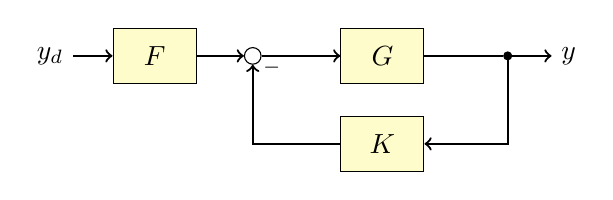
\begin{tikzpicture}
		\node (yd) {$y_d$};
		\node[block, right=0.5 of yd] (F) {$F$};
		\node[sum, right=0.6 of F] (sum) {};
		\node[block, right=of sum] (G) {$G$};
		\node[junction, right=of G] (out) {};
		\node[right=0.5 of out] (y) {$y$};
		\node[block, below=0.4 of G] (K) {$K$};
		
		\draw[connector] (yd) to (F);
		\draw[connector] (F) to (sum);
		\draw[connector] (sum) to (G);
		\draw[connector] (G) to (out) to (y);
		\draw[connector] (out) |- (K);
		\draw[connector] (K) -| node[right, pos=0.98] {$\scriptstyle -$} (sum);
	\end{tikzpicture}
	\caption{Controller split into feedforward block~($F$) and feedback block~($K$).}
	\label{fig:split_controller}
\end{figure}

Ignoring actuator saturation, we can get very high theoretical performance by carefully assigning costs to the outputs and the integrator, and the weights of the Kalman filter. Figure~\ref{fig:best_So} shows the singular values of the output sensitivity function for a fast controller.
The high bandwidth (above 100\,rad/s) guarantees a short rise time while the limited peak value (less than 2) provides a good stability margin.

\begin{figure}[htbp]
	\centering
	\includegraphics{chap10/best_So}
	\caption{Singular values of output sensitivity function for a fast controller designed ignoring actuator saturation.
		The dark blue line highlights the largest singular value.
		The red line is the upper bound corresponding to the performance specifications.
		The bandwidth is larger than 100\,rad/s, the peak is smaller than 6\,dB, and the attenuation at low frequencies is more than 40\,dB.
	}
	\label{fig:best_So}
\end{figure}

Figure~\ref{fig:best_y} shows the outputs of the closed-loop system while tracking a target when this controller is used to control the linearized reduced system without actuator saturation. The target is reached in about 25\,ms and there is no steady-state error.
However, the inputs requested to achieve this performance often exceed the saturation limits even in steady-state (Figure~\ref{fig:best_u}) because the integrator is working to bring the steady-state error to zero by requesting different inputs than those prescribed by the feedforward (which are within bounds).

\begin{figure}[htbp]
	\centering
	\includegraphics{chap10/fast_y_rotation}
	\includegraphics{chap10/fast_y_energy}
	\caption{Rotation measurements and stored energy over time while tracking a target for the linear system without actuator saturation.
		The target is reached in about 25\,ms and there is no steady-state error.
	}
	\label{fig:best_y}
\end{figure}

\begin{figure}[htbp]
	\centering
	\includegraphics{chap10/fast_u_current}
	\includegraphics{chap10/fast_u_beams}
	\caption{Coil current and NBI power over time while tracking a target for the linear system without actuator saturation.
		The inputs requested often exceed the saturation limits, even in steady-state.
	}
	\label{fig:best_u}
\end{figure}

We use this nominal controller as our reference for choosing performance specifications that must be met in the face of uncertainty.
It is standard to encode these specifications in a weight $W_P$ whose inverse forms an upper bound to the sensitivity function of the system.
For simplicity we choose $W_P$ diagonal with all diagonal elements equal to the inverse of the upper bound of the largest singular value of the sensitivity function.
The specifications are as follows: the bandwidth must be larger than 50\,rad/s with a -20\,dB/decade roll-off, and the peak of sensitivity must be less than 2 (6\,dB).
The corresponding upper bound for the sensitivity function is shown in red on Figure~\ref{fig:best_So}.
The closed-loop system formed using our nominal controller is stable and meets these specifications so we can now address robustness.



\paragraph{Robust Stability and Performance}

Next we want to introduce perturbations in our system.
Without data from NSTX-U, we choose to introduce parameter uncertainty.
The two parameters that are most likely to be varying significantly from their nominal value are $\chi_\phi$ and $\tau_E$.
Let $\bar{\chi}_\phi$ be the nominal value (which depends on the radial variable $\rho$) of $\chi_\phi$, and
let $\bar{\tau}_E$ be the nominal value of $\tau_E$.
We assume that the perturbed model $G_p$ is built from perturbed values of the parameters ${\chi_\phi}_p$ and ${\tau_E}_p$, where
${\chi_\phi}_p$ is a random perturbation of bounded magnitude around $\bar{\chi}_\phi$ generated using 1D Perlin noise, and ${\tau_E}_p = \mu \cdot \bar{\tau}_E$ for some $\mu$.
Let $\Pi$ be the set containing all such perturbed versions of our nominal model $G$.
Robust stability (resp. performance) is obtained when all plants in $\Pi$ are stable (resp. performant).

In order not to arbitrarily restrict the allowable magnitude of the perturbations, we start with a large range of allowed perturbations and progressively restrict the range until we get robust stability and performance.

To greatly simplify the analysis while being strictly conservative about stability and performance, we will use a \emph{norm-bounded} description of uncertainty where $\Pi$ is allowed to contain $\mathcal{H}_\infty$ norm-bounded perturbations of our nominal model $G$.
To determine the best way to integrate this uncertainty into our model, we superimpose the Nyquist plots of many perturbed plants and we observe that right multiplicative uncertainty adequately represents the pattern we obtain.
Thus we write
\begin{equation} \label{eq:multiplicative}
	G_p = G (I + \Delta W),
\end{equation}
where $W$ is a weighting transfer function matrix, and $\Delta$ satisfies $\|\Delta\|_\infty < 1$.
A block diagram of the perturbed plant is shown in Figure~\ref{fig:multiplicative}.

\begin{figure}[htbp]
	\centering
	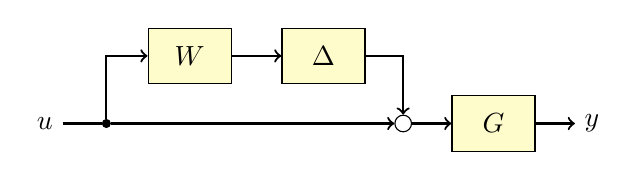
\begin{tikzpicture}
		\node (u) {$u$};
		\node[junction, right=0.5 of u] (in) {};
		\node[coordinate, right=1 of in] (below W) {};
		\node[block, above=0.5 of below W] (W) {$W$};
		\node[coordinate, right=1.7 of below W] (below Delta) {};
		\node[block, above=0.5 of below Delta] (Delta) {$\Delta$};
		\node[sum, right=0.9 of below Delta] (sum) {};
		\node[block, right=0.5 of sum] (G) {$G$};
		\node[right=0.5 of G] (y) {$y$};
		
		\draw[connector] (u) to (in) to (sum);
		\draw[connector] (sum) to (G);
		\draw[connector] (in) |- (W);
		\draw[connector] (W) to (Delta);
		\draw[connector] (Delta) -| (sum);
		\draw[connector] (G) to (y);
	\end{tikzpicture}
	\caption{Perturbed model $G_p = G (I + \Delta W)$}
	\label{fig:multiplicative}
\end{figure}

To find $W$, we first observe that $\Delta W = G^{-1}{G_p} - I$.
Thus we can superimpose the Bode plots of $G^{-1}{G_p} - I$ for many perturbed plants and choose a low-order upper bound which will prescribe $W$.
Note that $G^{-1}{G_p} - I$ and $W$ are matrices so we must find upper bounds for each element.

\begin{figure}
	\centering
	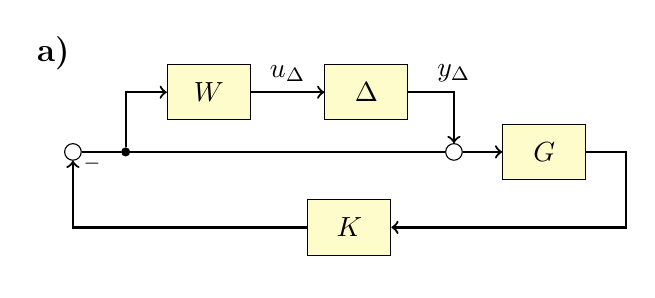
\begin{tikzpicture}
		\node[font=\large\bfseries] at (-0.25,1.25) {a)};
		\path (0,1.25) -- ++(down:2.75);

		\node[sum] (sum) {};
		\node[junction, right=0.5 of sum] (in) {};
		\node[coordinate, right=of in] (below W) {};
		\node[block, above=0.4 of below W] (W) {$W$};
		\node[coordinate, right=2 of below W] (below Delta) {};
		\node[block, above=0.4 of below Delta] (Delta) {$\Delta$};
		\node[sum, right=of below Delta] (out) {};
		\node[block, right=0.5 of out] (G) {$G$};
		\node[coordinate, right=0.5 of G] (end) {};
		\node[coordinate] (above K) at ($(sum)!0.5!(end)$) {};
		\node[block, below=0.6 of above K] (K) {$K$};
		
		\draw[connector] (sum) to (in) to (below W) to (below Delta) to (out) to (G);
		\draw[connector] (G) to (end) |- (K);
		\draw[connector] (K) -| node[right, pos=0.98] {$\scriptstyle -$} (sum);
		
		\draw[connector] (in) |- (W);
		\draw[connector] (W) to node[above] {$u_\Delta$} (Delta);
		\draw[connector] (Delta) -| node[above] {$y_\Delta$} (out);
	\end{tikzpicture}
	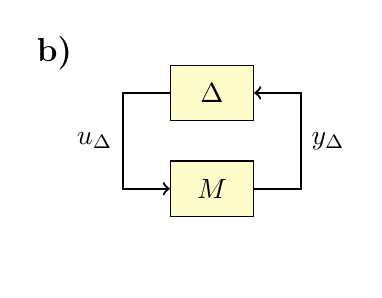
\begin{tikzpicture}
		\node[font=\large\bfseries] at (-2,0.5) {b)};
		\path (0,0.5) -- ++(down:2.75);
		
		\node[block] (Delta) {$\Delta$};
		\node[block, below=0.5 of Delta] (M) {$M$};
		
		\node[coord, right=0.6 of M] (right) {};
		\node[coord, left=0.6 of M] (left) {};
		
		\draw[connector] (M.east) to (right |- M) to node[right] {$y_\Delta$} (right |- Delta) to (Delta);
		\draw[connector] (Delta) to (left |- Delta) to node[left] {$u_\Delta$} (left |- M) to (M);
	\end{tikzpicture}

	\caption{Block diagrams of the loop of the perturbed closed-loop system stripped of all exogenous inputs and outputs. \textbf{a)} Expanded system. \textbf{d)} $M \Delta$ structure for robust stability analysis.}
	\label{fig:diagram_perturb}
\end{figure}

Now equipped with a mathematical description of our perturbed system, we can address robust stability.
Using block diagram algebra, we start by rearranging our system of Figure~\ref{fig:diagram_perturb}a into the $M \Delta$ configuration of Figure~\ref{fig:diagram_perturb}b to obtain the transfer function block matrix $M$:
\begin{equation}
	M = -W K S_o G.
\end{equation}

When the nominal closed-loop system is stable and when the largest singular value of $M$ is less than 1 for all frequencies, by theorem 8.4 of~\cite{SandP} (small-gain theorem), the closed-loop system is robustly stable.
We found that we could achieve robust stability for perturbations obtained from up to 10\% variations of the nominal parameters (Figure~\ref{fig:robust_stability}).

\begin{figure}[htbp]
	\centering
	\includegraphics{chap10/robust_stability}
	\caption{Robust stability. The singular values of $M$ are always less than 1.}
	\label{fig:robust_stability}
\end{figure}


To test for robust performance, we generate many perturbed plants and check that each one of them satisfies the performance specifications by superimposing the Bode plots of the largest singular value of all perturbed plants (Figure~\ref{fig:robust_performance}).
We verify that our controller has robust performance for the set of perturbed plants and the specifications stated above.

\begin{figure}[htbp]
	\centering
	\includegraphics{chap10/robust_performance}
	\caption{Robust performance.
		The singular values of the transfer functions of 256 perturbed plants are shown superimposed in blue.
		All perturbed transfer functions meet the performance specifications indicated by the upper bound in red.}
	\label{fig:robust_performance}
\end{figure}


\paragraph{Actuator saturation}

The controller studied above is fast at the expense of requiring large input values but also negative values which are impossible to produce in practice.
Introducing actuator saturation without otherwise modifying the controller does not work as the large and oscillatory requested input values drive the actual inputs to constantly saturate one way or another which is particularly ineffective at controlling the system as can be seen in Figures~\ref{fig:best_y_sat} and~\ref{fig:best_u_sat}.

\begin{figure}[htbp]
	\centering
	\includegraphics{chap10/fast_y_sat_aw_rotation}
	\includegraphics{chap10/fast_y_sat_aw_energy}
	\caption{Rotation measurements and stored energy over time while tracking a target with actuator saturation and the nominal controller designed above.
		The time response is erratic because the controller is requesting too large inputs which get saturated.}
	\label{fig:best_y_sat}
\end{figure}

\begin{figure}[htbp]
	\centering
	\includegraphics{chap10/fast_u_sat_aw_current}
	\includegraphics{chap10/fast_u_sat_aw_beams}
	\caption{Coil current and NBI power over time while tracking a target with actuator saturation and the nominal controller designed above.
		The beam powers are constantly saturating and sometimes jumping between their upper and lower limit.}
	\label{fig:best_u_sat}
\end{figure}


So instead we progressively reduce the weights assigned to the cost function until the input values get within reasonable bounds such that saturation only occurs for short durations, which allows us to obtain the best controller we can design in practice.
Note that since the saturation process is non-linear, we can no longer rely on linear control design tools like putting an upper bound on the sensitivity function for specifying performance specifications so we have to rely on time responses of the closed-loop system.
The closed-loop system exhibits a fast response time for sensor measurements (Figure~\ref{fig:good_y_sat}) while only saturating the inputs for a short time after a command is received (Figure~\ref{fig:good_u_sat}).
However, the time response for the stored energy is slower than for the rotation measurements and the target is not perfectly reached.
This is a design choice made to improve the tracking of the rotation at the expense of the stored energy.
Indeed, equation~\eqref{energy} imposes a trade-off between the stored energy and the beam powers by removing one degree of freedom in how the controller can set the inputs making it impossible to simultaneously and efficiently track both the rotation and the energy.

\begin{figure}[htbp]
	\centering
	\includegraphics{chap10/good_y_sat_rotation}
	\includegraphics{chap10/good_y_sat_energy}
	\caption{Rotation measurements and stored energy over time while tracking a target with actuator saturation and a controller designed to account for it.
		By design, the response is slower for the stored energy and the target is not perfectly reached.}
	\label{fig:good_y_sat}
\end{figure}

\begin{figure}[htbp]
	\centering
	\includegraphics{chap10/good_u_sat_current}
	\includegraphics{chap10/good_u_sat_beams}
	\caption{Coil current and NBI power over time while tracking a target with actuator saturation and a controller designed to account for it.
		Saturation only occurs for short periods during the transient.}
	\label{fig:good_u_sat}
\end{figure}

As shown in the next section, this controller works well in practice despite the additional burden of the full actuator constraints (saturation, PWM, limited on/off switches, refractory period) and the fact the the actual system to be controlled is non-linear.

\section{Simulation results} 

\label{results}

The goal of the simulations is to test the controller on both higher fidelity model (TRANSP) as well as the simplified reduced-order model.  The desired profiles shown in Figures~\ref{initnstxu} will the targets in both cases and the results will be presented to see the effectiveness of the controller.

\begin{figure}[htbp]
	\centering
	\includegraphics[width=0.7 \linewidth]{chap10/initial}
	\caption{Rotation profiles: definition of the initial profile, equilibrium profile $w_0$ used for the linearization and the desired profiles to reach $w_d$. The measurement points $r$ are the intersections of the different profiles with the measurement channels}
	\label{initnstxu}
\end{figure}

\subsection{Actuators constraints}
\label{constraintsnstxu}
Like in the NSTX device, the two different actuators (NTV coil current and NBI beam power) have constraints that need to be taken into account when applied on the real device (NSTX-U) through TRANSP. These constraints are made for the safety of the operations, they reflect the practicability and the feasibility of some requests to the device. The constraints will be added to the dynamics equations through restrictions on the actuators of the controller.

For the coil current, the restriction is only a limitation of its value between 0 and 3000 amperes.
The coil current response is so fast compared to the dynamics of the system that it can be assumed to be applied instantaneously (no lag between the controller action and its application).

For the NBI actuators in NSTX-U, each of the 6 beams has to be treated individually. Fusing the three beams of the first set was just a simplification in our model but because we apply the controller on TRANSP, each beam is coded separately and each beam can either be on and produce 2\,MW of power or off and produce 0\,MW.
In addition, each beam can only be switched off a maximum of 20 times per plasma discharge to prevent device fatigue issues, and there is a refractory period of 10\,ms after each switch on or off during which the beam cannot be switched again.
Also, due to diagnostic considerations, one NBI source is typically always on, and so the overall sum of the injected power is considered to be between $2$ and $12$\,MW.

These physical restrictions constrain the model and controller to be discrete and to use Pulse Width Modulation (PWM) for each beam power actuator in order to obtain the requested control values between 2 and 12\,MW.

\subsection{Computational approach  (TRANSP implementation)}

To predict the toroidal rotation and the stored energy for NSTX-U, TRANSP is running in a predictive mode for a given set of beam powers and coil current. It also takes as inputs models for the plasma boundary shape, plasma current, electron and ion (Chang-Hinton model~\cite{Changhinton}) temperature and density profiles and the momentum diffusivity coefficient.

The actuator commands required for closed-loop rotation and stored energy control simulations are entered into TRANSP, which serves as a plasma simulator for testing the present controller. For more details on the TRANSP implementation, see \cite{Boyer15}.

\subsection{Simulation on TRANSP}

The discretized controller is now applied to the reduced-order model and the TRANSP predictive model, considering all the constraints listed in Section~\ref{constraintsnstxu} for all the actuators and instead of applying the exact beam powers numerical value as requested by the controller, each of the 6 beams will be modulated individually while satisfying all the constraints. The coil current is limited by the value of $3000$ Amperes

At the beginning of each duty cycle, the controller sets the requested power. During the duty cycle, the beams switch on and off at most once to minimize the number of switches. Because of the 10\,ms refractory period and the limited switches, the exact requested power cannot always be met.

The longer the duty cycle, the better for the device because it means less commands switches so less fatigue, but a longer duration introduces a longer controller lag which impairs performance. A duration smaller than the refractory period is chosen for the duty cycle (6\,ms).

\begin{figure}
	\centering
	\begin{overpic}[width=0.8 \linewidth]{chap10/rotnstxu}
		\put(18,51){$\leftarrow$ Control on}
		\put(24.2,47){1st target}
		\put(55,51){Control on $\rightarrow$}
		\put(55,47){2nd target}
	\end{overpic}
	\caption{Comparison of the rotation measurements when PWM is applied for both the reduced-order model (red lines) and the TRANSP predictive model (blue lines).}
	\label{rotnstxu}
\end{figure}

\begin{figure}
	\centering
	\begin{overpic}[width=0.8 \linewidth]{chap10/energynstxu}
		\put(27,26){\tikz{
			\coordinate (O);
			\node (label) at (1,-1) {1st target};
			\draw[->,thick] (label) to (O);
		}}
		\put(77,41){\tikz{
			\coordinate (O);
			\node (label) at (1,1) {2nd target};
			\draw[->,thick] (label) to (O);
		}}
	\end{overpic}
	\caption{Stored energy measurements when PWM is applied for the TRANSP predictive model (blue line).}
	\label{energynstxu}
\end{figure}


\begin{figure}
	\centering
	\includegraphics[width=0.8 \linewidth]{chap10/currentnstxu} \adjustbox{raise=11em,lap=-0.8em}{(a)} \\[-0.5em]
	\begin{overpic}[width=0.8 \linewidth]{chap10/NBInstxu}
		\put(77,31){\tikz{
			\draw[thick,fill=white] (0,0.1) rectangle (3,2.4);
			\draw[ultra thick, blue] (0.1,2) -- (0.4,2);
			\node[anchor=west] at (0.4,2) {Beam set 1};
			\draw[ultra thick, red] (0.1,1.5) -- (0.4,1.5);
			\node[anchor=west] at (0.4,1.5) {Beam set 2A};
			\draw[ultra thick, black] (0.1,1) -- (0.4,1);
			\node[anchor=west] at (0.4,1) {Beam set 2B};
			\draw[ultra thick, green!50!black] (0.1,0.5) -- (0.4,0.5);
			\node[anchor=west] at (0.4,0.5) {Beam set 2C};
		}}
	\end{overpic} \adjustbox{raise=15.5em,lap=-0.8em}{(b)}
	\caption{Time evolution of the coil current and the beam power}
	\label{inputnstxu}
\end{figure}

Figure~\ref{rotnstxu} compares the rotation measurements when the PWM controller is applied to both the reduced-order model and the TRANSP predictive model in order to reach two targets, one at $t = 4.2$\,s, and the other starting at $t=4.6$\,s. Before $t=4.2$\,s, both models are not controlled (open loop).

Figure~\ref{energynstxu} represents the corresponding TRANSP predictive stored energy measurement.
At $t = 4.2$\,s a target of $0.55$\,MJ is reached then at $t=4.6$\,s another target of $0.65$\,MJ is reached.

The oscillations in both figures are due to the modulations that occur on each of the beam power source. The different beam power sources are represented in Figure~\ref{inputnstxu}(b) and the corresponding coil current in (Figure~\ref{inputnstxu}(a)). 

When at $t = 4.2$\,s we close the loop, the coil current saturates immediately to enable the rotation profile to drop quickly from its high initial state (all beams on) to the first desired rotation profile, then compensates for when the beam power is too high in order to decrease both the toroidal rotation and the stored energy and thus limit the overshoot. We thus reach the desired rotation and energy targets within the momentum diffusion time ($0.1$\,s).

The resulting measurements are very oscillatory but their amplitudes are damped and measurements from the reduced-order model are very close to those from TRANSP which again shows that the simplified model gives us a good qualitative approximation of the TRANSP rotation and energy prediction model.

\section{Summary and conclusions}
\label{conclusions10}

A ``model-based'' model of the plasma toroidal rotation and stored energy has been developed. The model is linear, and validations show good agreement between  model  predictions  and  actual  TRANSP predictive simulations.

The closed loop feedback system incorporates the delays and time constraints of the physical actuators, mainly the beam power actuators, and the results obtained using TRANSP simulations show promising time behavior, especially with the demonstration of the controller robustness in stability and performances.

Results predicted from the TRANSP simulations will be used to define the operating feedback system within the PCS. Simultaneous PCS feedback control of the plasma stored energy and rotation will enable exploration of new physics regimes in experiments on the NSTX-U machine.


This work was supported by the U.S. Department of Energy under contract No. DE-AC02-09CH11466 (PPPL) and U.S. Department of Energy  grant number DE-FG02-99ER54524 (Columbia University). 






% Make the bibliography single spaced
\singlespacing
\bibliographystyle{plainnat}

% add the Bibliography to the Table of Contents
\cleardoublepage
\ifdefined\phantomsection
  \phantomsection  % makes hyperref recognize this section properly for pdf link
\else
\fi
\addcontentsline{toc}{chapter}{Bibliography}

% include your .bib file
\bibliography{thesis}
%\bibliography{thesis}
\end{document}

